% https://github.com/uio-latex/phduio-article-based
% localdefs

\newcommand{\ctext}[3][RGB]{%
  \begingroup
  \definecolor{hlcolor}{#1}{#2}\sethlcolor{hlcolor}%
  \hl{#3}%
  \endgroup
}


%end local defs

% Add [final] to remove marginal notes,
% remove [colophon] for a blank colophon page:
\documentclass[colophon, english]{phduio}

\usepackage{phdstyle}   % Custom style
\usepackage{kantlipsum} % Dummy text

\author{Francesco Andreace}
\title{\kmers to rule them all}
\subtitle{Analysis of human pangenome graphs and other k-mer-based applications}
\department{Department of Computational Biology}
\faculty{Insitut Pasteur Paris, Universite' de Paris Cite}
\affiliation
{
    Edite doctoral school, Sorbonne Université
}
\ISSN{1234-5678}           
\dissertationseries{1234}  


\includeonly
{
    sections/dedication,
    sections/preface,
    sections/abstract-en,
    sections/abstract-no,
    sections/papers,
    sections/introduction,
    sections/background,
    sections/cqf,
    sections/paperI,
    sections/paperII,
    sections/paperIII,
    sections/appendixA,
    sections/appendixB,
    sections/perspectives,
    sections/conclusions,
    sections/pushing_the_limit,
    sections/reducing_complexity,
    sections/explorations
}


\begin{document}

    \frontmatter        % Folios in Roman numerals, unnumbered chapters.

    \maintitle

    \thispagestyle{empty}
\vspace*{\stretch{1}}
\begin{flushright}
    \emph{A qualche persona}
    %To those born and living in lands where poverty and conflict have robbed them of their fundamental right to education.
\end{flushright}

\vspace*{\stretch{3}}
    % \chapter{\abstractname}

All PhD theses must have two scientific summaries/abstracts:
One in Norwegian and one in English (it can be the same text).
The summaries/abstracts should be up to two pages (600--1200 words) and must be included in the thesis at the time of submission.
If you need assistance for the Norwegian summary, contact your supervisor/research group.
As a last resort, you could use Semantix Translations (\url{www.semantix.no}).
Please contact Semantix in order to get a quote.

Automatic \enquote{quotation marks} and cross-references are handled correctly for the specified language.

\todo[inline]{Add new section about results in \cref{sec:fourth}.}
    % \begin{otherlanguage}{norsk}
\chapter{\abstractname}

Alle avhandlinger skal ha to vitenskapelig sammendrag:
Ett norsk og ett engelsk (det kan være samme tekst).
Sammendragene skal være på inntil to sider (600--1200 ord).
Sammendragene skal være inkludert i avhandlingen på innleveringtidspunktet.
Dersom du trenger hjelp med sammendraget på norsk, ta kontakt med din veileder/forskningsgruppe.
I siste instans kan du ta kontakt med Semantix Translation Norway (\url{www.semantix.no}) for å få et tilbud.

Automatiske \enquote{anførselstegn} og kryssreferanser håndteres riktig for det gjeldende språket.

\todo[inline]{Legg til ny seksjon om resultatene i \cref{sec:fourth}.}

\end{otherlanguage}
    \chapter{Preface}
This thesis is submitted in partial fulfillment of the requirements for the degree of \emph{Philosophiae Doctor} at \sorbonne.
The research presented here was conducted at the \pasteur, under the supervision of Dr. Rayan Chikhi and Dr. Yoann Dufresne.
This work was mainly supported by the European Union’s Horizon 2020 research and innovation program under the Marie Skłodowska-Curie grant agreement No \num{956229} (+Panagaia +Pasteur + INCEPTION).

This thesis is a collection of some of the different projects I worked on during my stay at \pasteur. I begin with an small foreword of the research output of my PhD, and a gentle introduction of the scientific background needed to contextualize the work proposed in the manuscript. In the first part I present the published paper I am first author of, together with other unpublished work I lead or independently developed. In the second part I present other results of my scientific production, with novel elaboration of the work that appeared in the other papers I am co-author and presentation of projects that have or will be submitted to revision.
The common theme is human pangenomics and computational methods used to generate and use such models to infer relevant information.  
This essay ends with a chapter showcasing future perspectives and conclusions.

\section*{Acknowledgements}
First and foremost, I would like to express my deepest gratitude to Rayan for his constant support, patience, encouragement, and understanding throughout this journey. His ability to bring value to our work, his admirable work ethic, and the scientific intelligence he demonstrated in all the fields we discussed have been a true source of inspiration. I am truly fortunate to have had the opportunity to learn from him.\\
I would also like to extend my deepest gratitude to Yoann, who has been a constant source of motivation and inspiration throughout this journey. His passion for his work has been truly contagious, fueling my own interest in this field. Yoann not only helped me significantly improve my computer science skills but also became a valued person in my life in Paris. Whether it was inviting me to events at La Treso, patiently teaching me French alongside Pierre, explaining me the technicalities of the game he invesnts, talking about politics or inviting me for runs, his presence enriched both my personal and professional experiences.\\
A heartfelt thanks goes to François Sabot and Matthias Zytnicki for kindly agreeing to review this manuscript and for devoting their time and effort to being part of the thesis jury. I understand the significant commitment involved, and I deeply appreciate their contributions.\\
I extend my sincere thanks to Paola Bonizzoni, Camille Marchet, and Pierre Peterlongo for serving as members of the jury. Each one of you has played a special role in the trajectory of my thesis for particular reasons, and I am immensely grateful for your presence today as examiners.\\
Additionally, I wish to express my appreciation to Pierre Peterlongo and Martin Weigt for being part of my Comité de Thèse, offering valuable feedback that greatly contributed to the successful completion of this project.\\
To the SeqBio group, I would like to extend a special thank you. The group is composed of remarkable individuals, and I am lucky to have been part of it. In particular, I want to thank Camila for always being there to talk things through and for offering invaluable advice. I am equally grateful to Yoshihiro for his kindness and willingness to help in any circumstance and to Mélanie, whose support during every “chat noir” situation ensured I could finish this PhD.\\
I want to express deep gratitude to the Italian and Spanish community in Pasteur, who made me feel at home in every moment of these 40 months.\\
Lastly, I would like to thank the Alpacas, a distinguished group of young scientists, but even more importantly, incredible people. It has been such a pleasure to work and spend time with all of you.\\

%Finalmente, quiero agradecer a mi Belsy,\\
%Voglio inoltre ringraziare la mia famiglia. \\
%A mia madre, che mi ha sempre insegnato a rispettare gli altri e ad essere una persona corretta in questo mondo. Che ha speso anima e corpo quando non sono stato bene e che si preoccupa ancora, come ogni madre italiana che si rispetti, di suo figlio.\\
%A mia sorella, che mi ha insegnato a non accontentarmi e a puntare sempre in alto.\\
%A mio padre, che mi ha trasmesso la passione per l'informatica.\\
%A mia nonna, il cui amore e bonta' mi riempiono il cuore ogni volta in cui stiamo assieme. \\
%A mio nonno, che se ne e' andato poco prima che partissi per questo dottorato, e che rimarra' sempre nel mio cuore.\\
%I would finally like to thank my friends, in Italy, Paris and abroad, who took care of me and made me enjoy my life. \\
\vskip\onelineskip
\begin{flushleft}
    \sffamily
    \textbf{\theauthor}
    \\
    Paris,\MONTH\the\year
\end{flushleft}
    %\chapter{List of Papers}

% PANGENOMICS

\section*{Comparing methods for constructing and representing human pangenome graphs}
Francesco Andreace, Pierre Lechat, Yoann Dufresne, and Rayan Chikhi
\enquote{}.
In: \emph{Genome biology}.
Vol.\ 24,
no.\ 1
(2023),
pp.~274.
\doi{10.1186/s13059-023-03098-2}.

% BQF
\section*{The Backpack Quotient Filter: a dynamic and space-efficient data structure for querying k-mers with abundance}
Victor Levallois, Francesco Andreace, Bertrand Le Gal, Yoann Dufresne,Pierre Peterlongo.
In: \emph{iScience}.
Vol.\ TOFILL,
no.\ TOFILL
(2024),
pp.~TOFILL.
\doi{TOFILL}.

% MUSET

\section*{MUSET: Set of utilities for the construction of abundance unitig matrices from sequencing data}
Riccardo Vicedomini, Francesco Andreace, Yoann Dufresne, Rayan Chikhi and Camila Duitama Gonzalez 
\enquote{}.
In: \emph{Bioinformatics}.
Vol.\ TOFILL,
no.\ TOFILL
(2024),
pp.TOFILL.
\doi{TOFILL}.

% METAGENOMIC PRIMER
\section*{Analysis of metagenomic data}
TOFILL
\enquote{}.
In: \emph{Nature Reviews Methods Primers}.
Vol.\ TOFILL,
no.\ TOFILL
(2024),
pp.TOFILL.
\doi{TOFILL}.

% BACK_TO_SEQUENCES

\section*{Back to Sequences: Find the origin of \kmers}
Anthony Baire, Pierre Marijon, Francesco Andreace, and Pierre
Peterlongo 
\enquote{}.
In: \emph{Journal of Open Source Software}.
Vol.\ 9,
no.\ 101
(2024),
pp.~7066.
\doi{10.21105/joss.07066}.


% HACKATON 

\section*{SV pangenome hackaton}
TOFILL
\enquote{}.
In: \emph{TOFILL}.
Vol.\ TOFILL,
no.\ TOFILL
(2024),
pp.TOFILL.
\doi{TOFILL}.

    \cleartorecto
    \microtypesetup{protrusion = false}
    \tableofcontents    % Or \tableofcontents*
    \cleartorecto
    \listoffigures      % Or \listoffigures*
    \cleartorecto
    \listoftables       % Or \listoftables*
    \microtypesetup{protrusion = true}

    \mainmatter         % Folios in Arabic numerals, numbered chapters.

    %\chapter{Introduction}
\label{sec:intro}
As sequencing technology becomes increasingly accessible and accurate, the production of high-quality genome assemblies for organisms of the same species is accelerating. The contrast in processing time is stark: while the Human Genome Project took 13 years to produce its results in 2003, hundreds of genomes of similar quality are now being produced within a few years. Large-scale initiatives such as the UK Biobank, which has sequenced the genomes of 100,000 individuals, present new challenges in efficiently analyzing genetic data from relatively similar populations.\\
Traditionally, genomics software has been developed under the assumption that only one or a few high-quality reference sequences of a single species were available for analyzing limited amounts of new data. Consequently, the wealth of newly available public information is not being fully utilized to enhance the quality of current studies. Furthermore, the velocity and heterogeneity of new sequences deposited in public databases like ENA or SRA render current algorithms inadequate for rapidly analyzing population data that can be inferred from them.\\
To address these limitations, a transformative approach known as pangenomics is emerging. Pangenomics aims to reduce the observational bias inherent in current genomic analyses by capturing the entire genetic diversity within a single population, species, or group of similar organisms into a complex representation called a pangenome. This approach necessitates the development of novel computational methods capable of processing thousands of large and complex genomes.\\
As the field of computational pangenomics is relatively new, there is currently no one-size-fits-all solution that satisfies all requirements and enables straightforward downstream analysis for all genomic applications. Different models are being explored to address various challenges in representing, indexing, compressing, and analyzing pangenomic data.\\
One model gaining significant attention is an improvement on the sequence graph, called a variation graph, which models relationships between shared parts and differences in genomes using nodes and edges. Alternatively, an established method for efficiently representing genomic data involves decomposing variable-length sequences, known as reads, into fixed-size tokens called \kmers. The term \kmer derives from the use of an arbitrary value, $k$, which represents the fixed length of these tokens.\\
The \kmer model has demonstrated its effectiveness in numerous bioinformatics techniques, particularly in assembling genomes from reads of a specific species. More recently, \kmers have gained popularity by enabling superior processing of complex data such as ancient DNA or metagenomes from marine samples compared to other methods. Various data structures have been proposed to represent sequencing data as sets of \kmers, each with its own strengths and limitations.\\
As the field of pangenomics continues to evolve, researchers are exploring and refining these different approaches to develop more comprehensive and efficient methods for analyzing the vast amounts of genomic data being generated. The ultimate goal is to create tools and techniques that can fully leverage the wealth of genomic information now available, leading to more accurate and insightful analyses of genetic diversity within and across species.\\
\section{Research Output}
In this dissertation I present the result of my work on analyzing, developing and applying computational methods, mostly \kmer based, for \pangenomics. In the 40 months I spent at the Institut Pasteur under the supervision of Rayan Chikhi and Yoann Dufresne, I have contributed to several projects on \kmer based data structures and pursued my own research direction on pangenomics.\\
This has resulted in several publications, including one as first author and two as second author. At the moment of the writing of this manuscript I also expect to be author of other articles based on the work presented here.\\
In these years I have been involved in oral and poster presentations, mainly at events related to the Marie-Curie ITN network I have been part of.\\
Finally, by being part of the student association at Pasteur, I have been involved in several outreach events, as the European Researcher Night, to broadly present the bioinformatics and genomics research fields.
\section{General Outline}
The manuscript is organized as follows:
\begin{itemize}
	\item[\textbf{Chapter 2}] An introduction to the subject of the thesis and outline of the manuscript.
	\item[\textbf{Chapter 3}] An introduction of the background concepts of Genomics and Pangenomics.
	\item[\textbf{Chapter 4}] This chapter is structured into two main sections. The first section presents my work on human pangenome graph representation, detailing the methodologies employed and the insights gained from this research. This work contributes to the current efforts to create more comprehensive and accurate representations of human genetic diversity. \\The second section addresses the challenges associated with constructing pangenomes that represent cross-chromosome events in yeast. It explores the complexities of capturing genetic variations that span multiple chromosomes, a particularly challenging aspect of pangenome graphs construction.
	\item[\textbf{Chapter 5}] Presentation of three \kmer based methods to which I contributed. The chapter begins with a concise overview of the current state of the art. It is then divided into three separate sections, each providing a detailed discussion of the respective method, including its underlying principles, implementation details, and the specific contributions.
	\item[\textbf{Chapter 6}] Perspectives.
	\item[\textbf{Chapter 7}] Conclusions.
\end{itemize}

%As sequencing is every day more accessible in terms of cost and better in terms of accuracy, increasingly more high quality assemblies are being produced for organisms of the same species. This is also coming at lower processing time: the Human Genome Project took 13 years to produce its result in 2003, while now genomes of similar quality are being produced by the hundreds in a few years time. In addition to this, Project like the UK BioBank, which sequenced the genome of 100 thousands people, pose the challenge of how to efficiently analyze jointly all the genetic data of a relatively similar population.
%Genomics software has been developed under the assumption that only one or few top grade sequences of a single species were available as reference to help analyzing relatively limited amount of new data. This means the new publicly available information is currently not used to improve the quality of present studies. Moreover, the velocity and heterogeneity of new sequences deposited in public databases, like ENA or SRA, makes current algorithms unfit to jointly analyze rapidly the population data that can be inferred from them. 
%For this reason, a new transformative approach is emerging beyond the single reference genome: \pangenomics.
%Its aim is to reduce the observational bias of current genomic analyses by capturing the entire genetic diversity within a single population, species or group of similar ones, into a complex representation called \pangenome.
%To do so, novel computational methods are therefore needed to process up to thousands large and complex genomes. As the research field of computational \pangenomics is relatively new, at the present moment there is no one-fit-all solution that satisfies the requirements and enable straightforward downstream analysis for all genomics applications. In fact, different models are being used to tackle the various problem of representing, indexing, compressing and 
%The model that is currently more researched is an improvement of a sequence graph, called variation graph, in which relationship between shared parts and differences in genomes are modeled by nodes and edges.
%Alternately, one known way of efficiently represent genomic data is to decompose sequences of variable length, known as reads, into tokens of fixed size, called \kmers. This name comes from the use of an arbitrary value, namely \emph{k}, that is the fixed length of such tokens. The \kmer model has proven its effectiveness in many bioinformatics techniques and particularly for assembling genomes from reads of a particular species. More recently they are gaining success by enabling superior processing of complex data such as ancient DNA or metagenomes from marine samples compared to other methods. Many data structures have been proposed to represent sequencing data into sets of \kmers, each of them with its strengths and limitations.
%In this dissertation I present my work on analyzing, developing and applying computational methods, mostly \kmer based, for \pangenomics. 


%publicly available genomic data has already grown past the peta-base scale.
%New tools are being developed to process such extraordinary wealth of information to efficiently store it and to enable practical analysis and exploration of it.
%One of the most promising way of representing it is to decompose the produced sequences of variable length, known as reads, into tokens of fixed size, called \kmers. This name comes from the use of an arbitrary value, namely \emph{k}, that is the fixed length of such tokens. The \kmer model has proven its effectiveness in many bioinformatics techniques and particularly for assembling genomes from reads of a particular species. More recently they are gaining success by enabling superior processing of complex data such as ancient DNA or metagenomes from marine samples compared to other methods. Many data structures have been proposed to represent sequencing data into sets of \kmers, both coming from one or multiple samples, together with useful metadata like occurrence counts or the sample of provenience. Each of them has its strengths and limitations. At the present moment there is still no one-fits-all solution that is able to represent perfect lossless information from the input data while being extremely efficient computationally and primed for ease of use on downstream applications. In this dissertation I present my work on analysing, developing and using \kmer based methods to represent complex datasets containing multiple samples or individuals. These methods are of use in a novel genomics area called pangenomics, that considers multiple sequences together to infer a more comprehensive picture of the genetic diveristy and richness of a species.
%They also help efficient information retrieval for very complex environmental samples, in which the the challenge is to correctly pull apart the collapsed sequencing information to reconstruct and differentiate the genetic information of the wide variety of organisms present in it.
    %\section{DNA, genome variation and sequencing data}
\label{sec:background:sequencing}
A fundamental grasp of the data that is produced by sequencing biological organisms is essential to comprehend the research outlined in this manuscript. If already familiar with DNA sequences, how they are obtained and how they differ between species or individuals, you may proceed to section~\ref{sec:background:pangenomics}.
\subsection{DNA}
DNA (Deoxyribonucleic Acid) is a complex molecule with a double helix structure that carries the genetic information of an organism. Although its discovery was the result of work by many scientists over nearly 90 years, the currently accepted model was first correctly described by James Watson and Francis Crick in 1953 at Cambridge, UK.\\
The information DNA carries provides instructions for an organism to develop, survive in the external world, and reproduce. These instructions are encoded as a sequence of monomers called nucleotides. Each nucleotide is composed of a sugar, a phosphate group, and one of four nucleobases: cytosine, guanine, adenine, and thymine. The nucleotides are commonly referred to using the first letter of their nucleobases: A, C, G, and T. In RNA molecules, thymine is replaced by uracil.\\
The nucleotides are linked together in a sugar-phosphate backbone. Hydrogen bonds between complementary nucleotides form the molecule's double-stranded structure, with A pairing with T and C pairing with G bases. This pairing is crucial for DNA replication and protein synthesis. Figure~\ref{fig:DNA} shows the structure of the DNA molecule and the nucleotides, with the initial drawing by Francis Crick in 1953.
\begin{figure}[h!]
	\centering
	\begin{subfigure}[b]{0.95\textwidth}
		\centering
		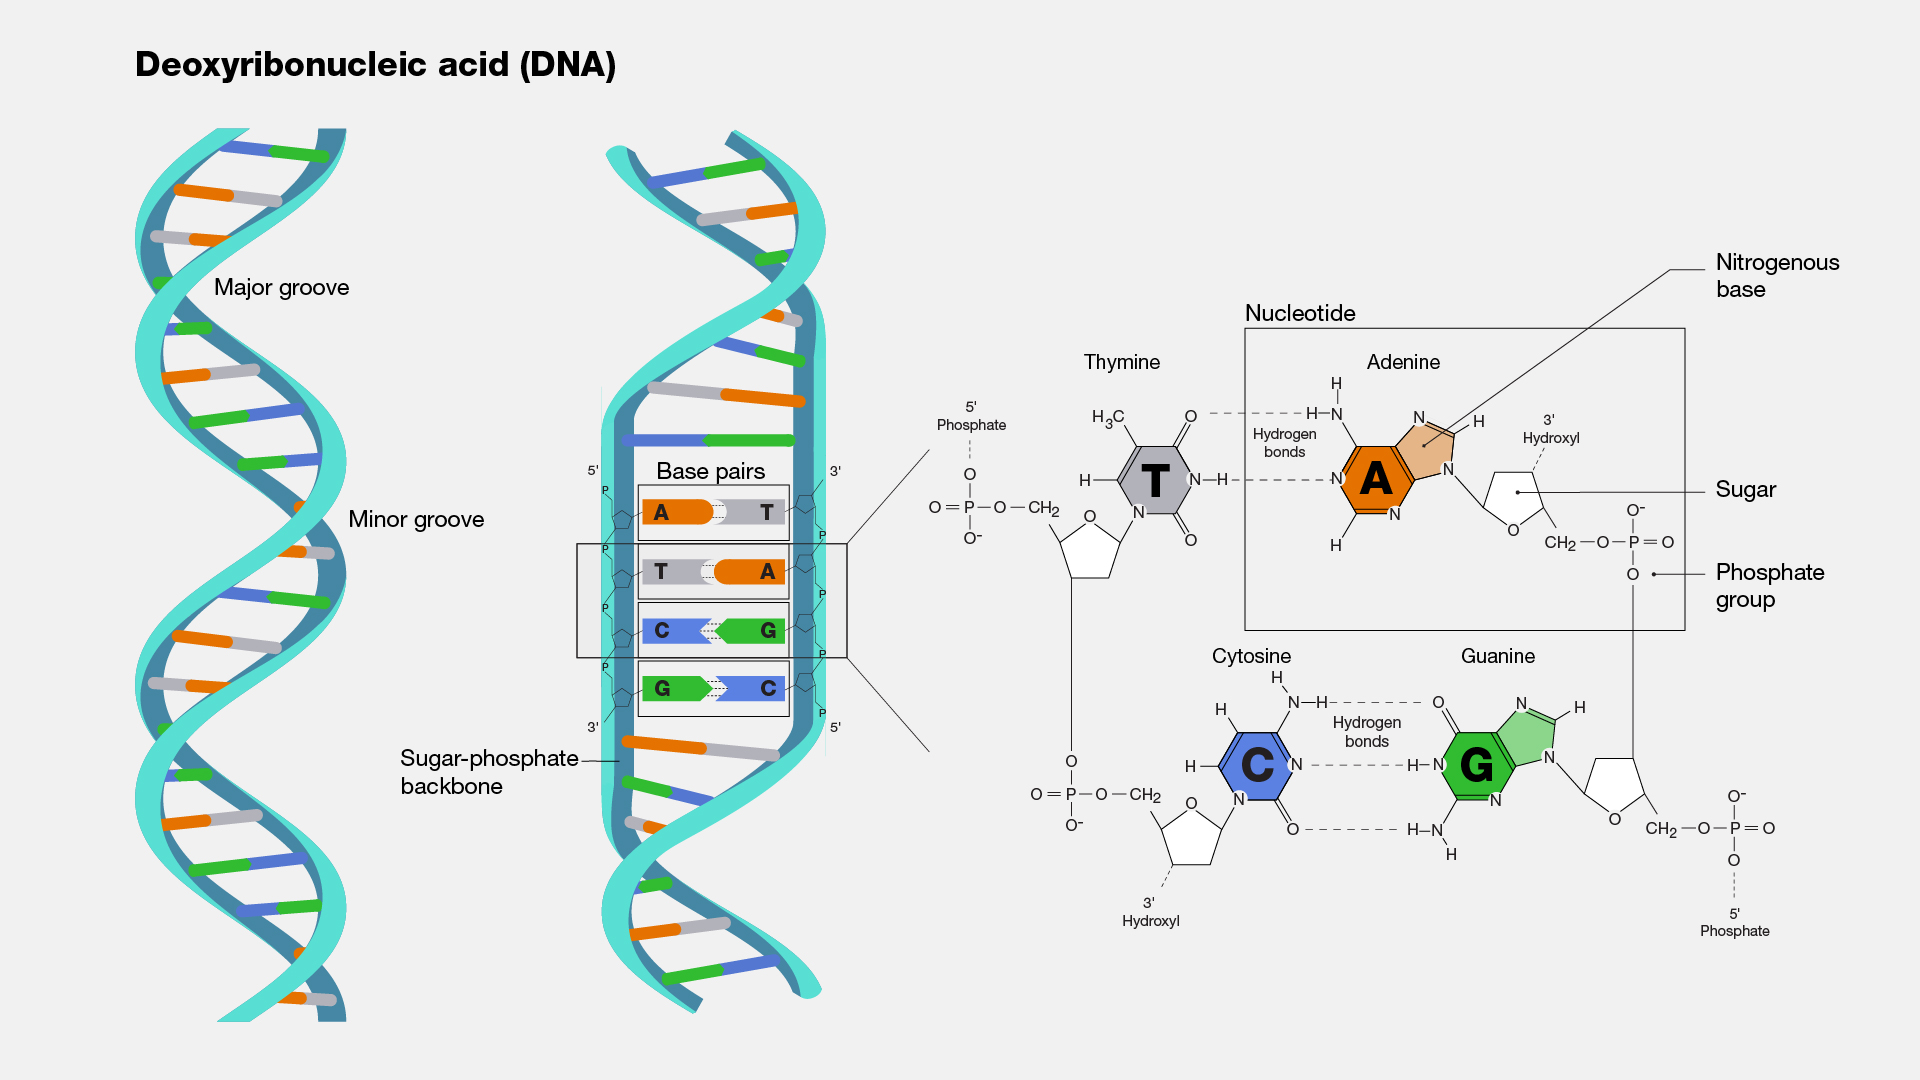
\includegraphics[width=0.95\textwidth]{figures/background/DNA_2024a.jpg}
		\caption[The DNA molecule]{The DNA molecule and the structure of the nucleotides, the basic piece of information of the DNA. Figure from NIH glossary~\cite{nih_dna}.} 
	\end{subfigure}%
	\\
	\begin{subfigure}[b]{0.75\textwidth}
		\centering
		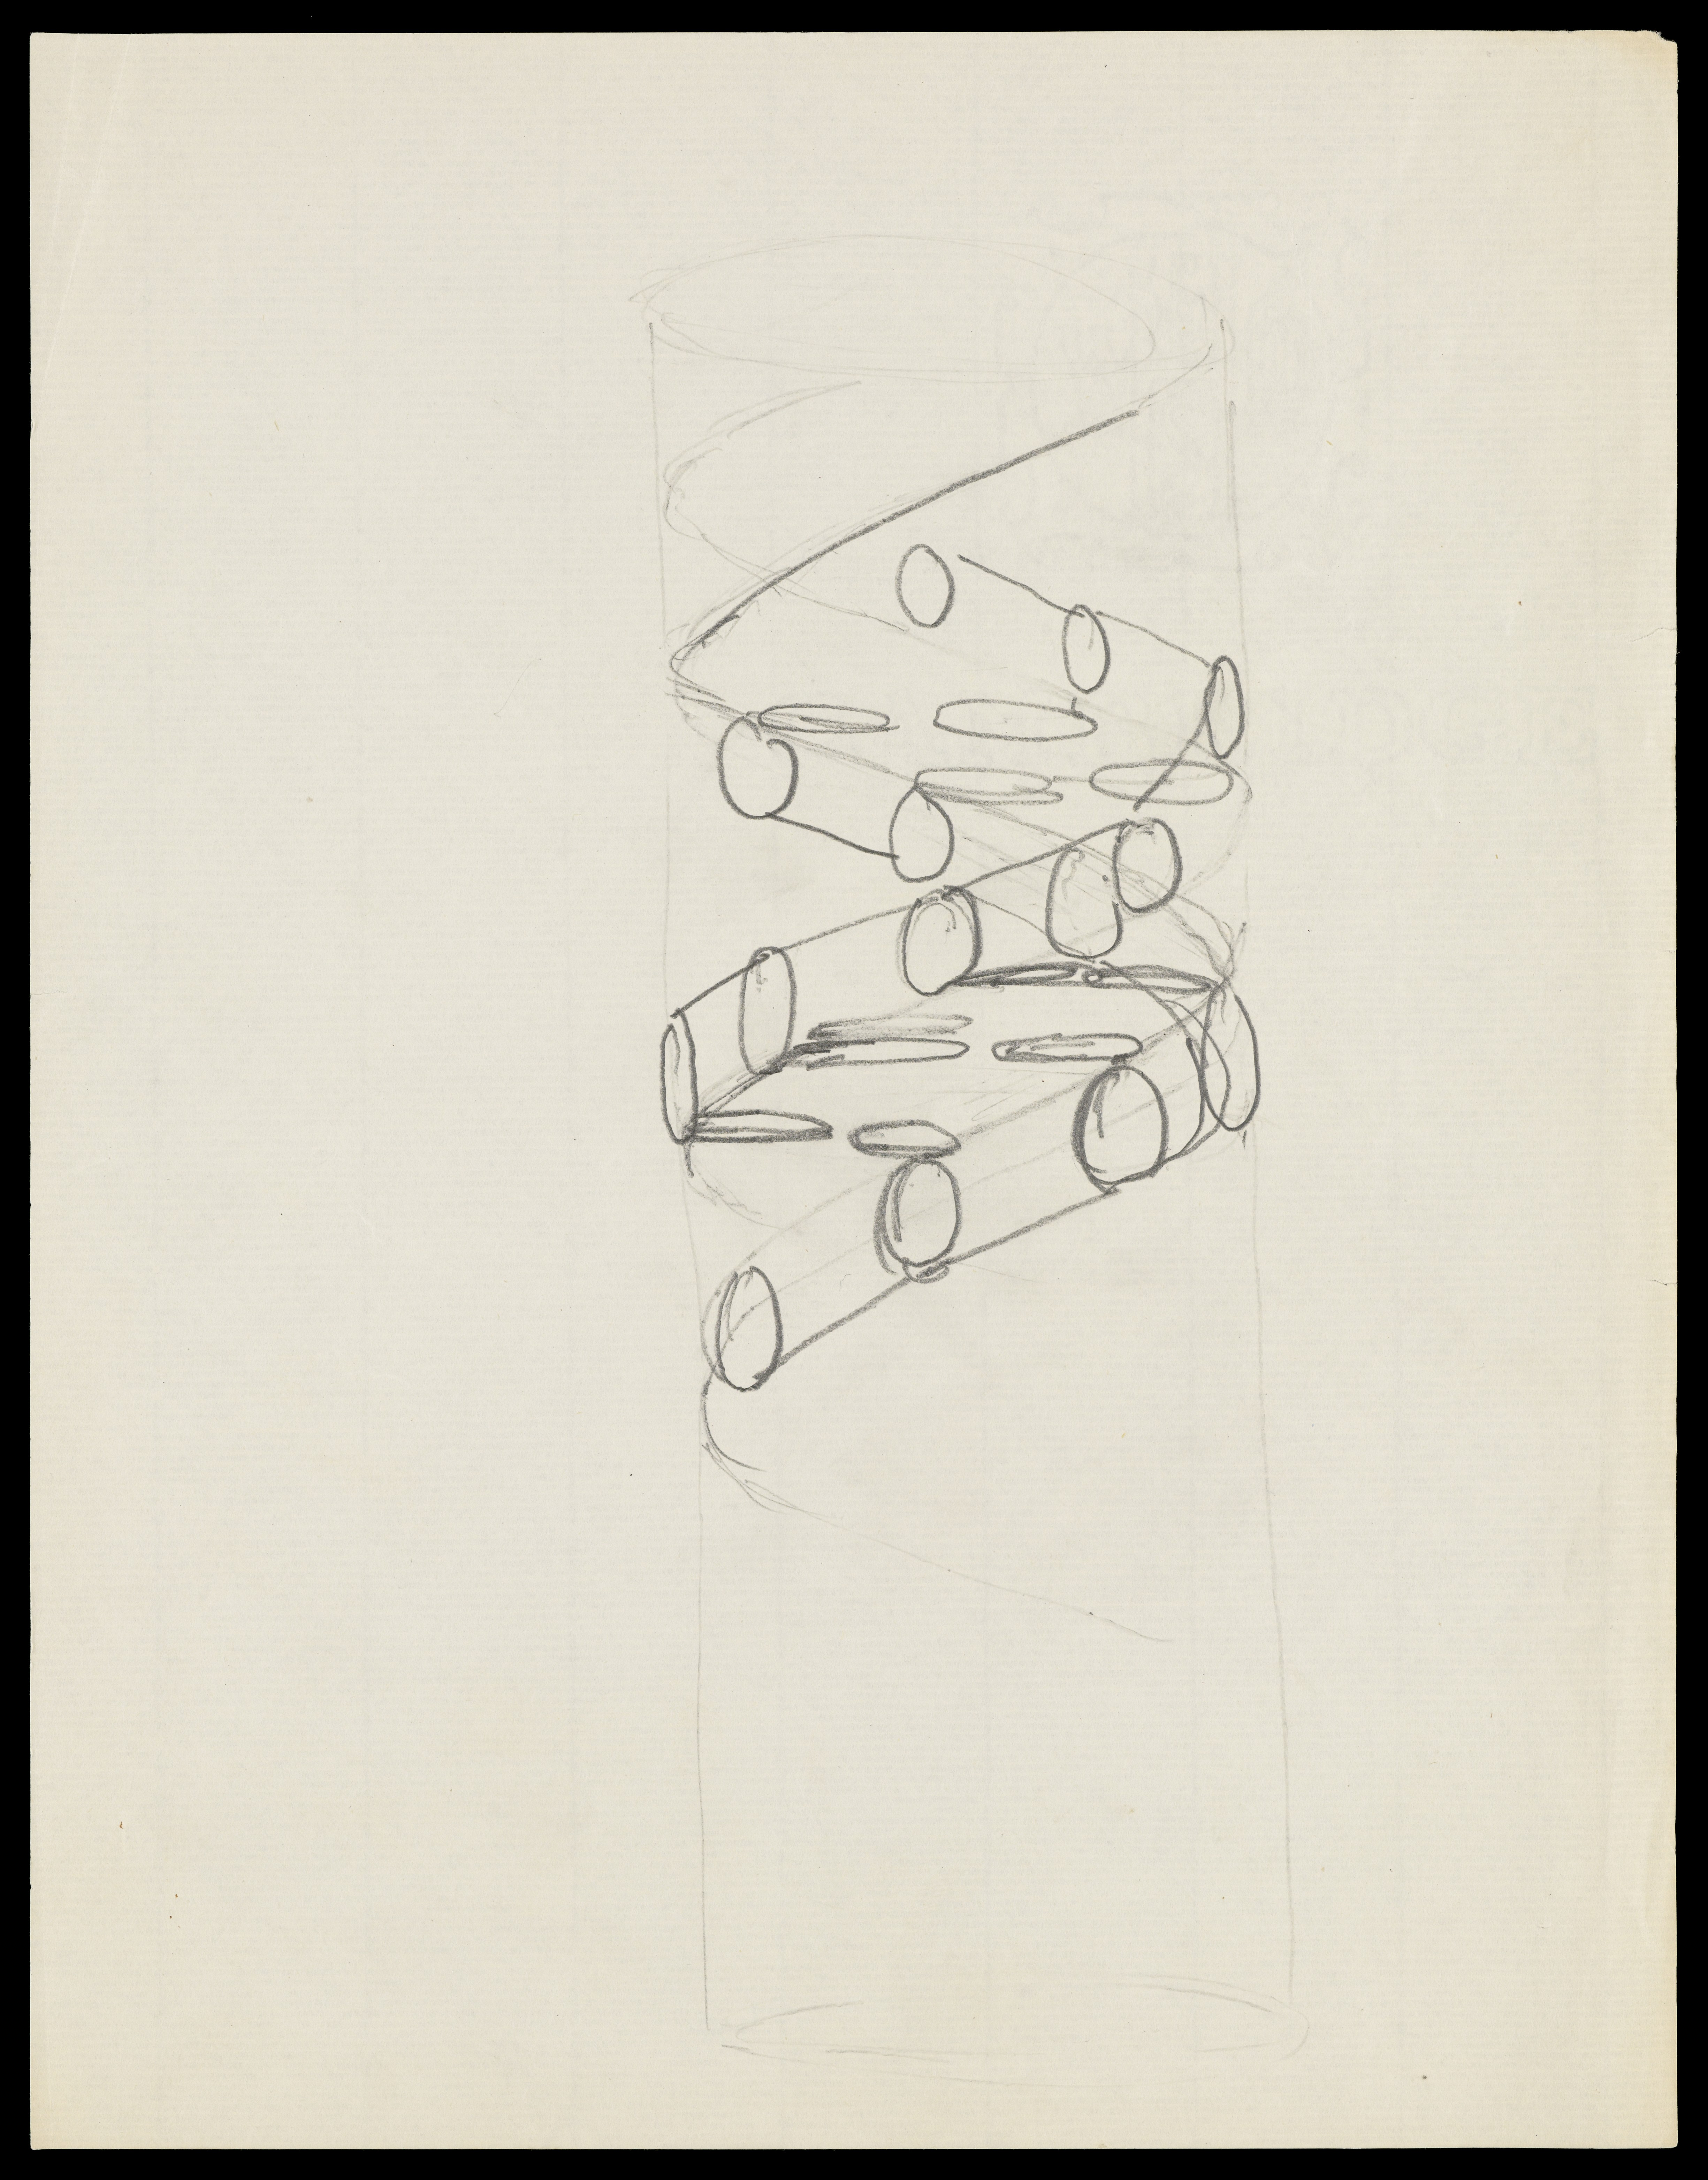
\includegraphics[width=0.5\textwidth]{figures/background/DNA_sketch.jpg}
		\caption[The DNA sketch by Crick]{The DNA molecule model draw by Francis Crick in 1953.} 
	\end{subfigure}%
\caption{The DNA molecule.}
\label{fig:DNA}
\end{figure}

To fit inside the cell nucleus, DNA is organized in very tight structures. First is coiled around proteins called histones to from a compact structure called chromatin that form loops and is kept in place by other molecules to structure a chromosome. In humans, each nucleus contains 23 chromosome pairs. 22 are the autosomes, i.e. the chromosomes we all have and that are not associated with sex, while the last pair is the sex one that contains or 2 copies of chromosome X for women or 1 X and 1 Y for men. The final part of the chromosome is called telomere while the central one is called centromere and both are regions known to contain a lot of repetitive regions that are very difficult to reconstruct from sequencing. \\ Finally, there is also the mitochondrial genome, that is not in the nucleus, has circular structure and is mostly inherited maternally.

\subsection{DNA sequencing}
In many biological disciplines, studying an organism's genetic information contained in its DNA is crucial. Over the years, researchers have developed various methods and techniques to extract this information from the cell nucleus and to represent it in a useful way. These processes typically involve three main steps. Here I describe them, with many simplifications, to give a brief overview:
\begin{itemize}[leftmargin=1.8cm]
	\item[\textbf{Library preparation}] The first step requires hours long, nontrivial biological manipulation of samples to extract DNA from cell nucleus and purify it without causing damage. This process isolates the genetic material from other cellular components, like RNA and proteins. The DNA molecule are fragmented into pieces of different length followed by $5\prime$ and $3\prime$ adapter ligation. Some technologies require PCR amplification of fragments, while others don't.
	\item[\textbf{Sequencing}] Next, specialized machines detect the sequence of nucleotides that compose the extracted DNA pieces. These techniques, called sequencing, use various, most of the time proprietary, technologies to determine the precise order of nucleotides (A, C, G, and T) in a DNA molecule. The raw data output of these machines are sequences of characters that are referred to as sequencing reads or simply reads.
	\item[\textbf{Analysis}] In this step usually quality control (QC) is performed to remove adapters and too short or low quality reads. Usually the first step after QC is to assemble the sequences together or to provide them as input to a workflow specific for the required application.
\end{itemize}
The landscape of DNA sequencing has evolved significantly since its inception. In 1977, Frederick Sanger and his colleagues introduced the first widely adopted sequencing method, known as chain termination sequencing or Sanger sequencing\cite{sanger_sequencing}. This technique allowed to read the sequence of nucleotides in a DNA molecule for the first time in a reliable and reproducible manner. This was the technique that led to the first sequencing of the mitochondrial DNA and the first ,almost, complete human genome in 2001~\cite{mitochondrialDNA,first_human_genome}.
While Sanger sequencing has revolutionized genetic research, it has largely been replaced by more advanced technologies. These newer methods fall into two main categories: Next Generation Sequencing (NGS) and Third Generation Sequencing. These technologies provide significant improvements in terms of speed, cost-effectiveness and data output compared to Sanger sequencing. \\
\subsubsection{Next Generation Sequencing} derives its name by launching a so-called next generation by revolutionizing sequencing with massive parallelization. This technology has continuously improved since 2005 to yield up to 8 Terabases per single sequencing run, taking it maximum 2 days and dropping the price of, for example, a single individual sequenced per almost 100 dollars~\cite{100dollars}. The advancement consists mainly in running many reactions and analysis in parallel to produce millions to billions of reads of a length that varies between 150 and 300 bases. For this reason they take the name of short reads. While a big advantage of this sequencing method is the low error rates, with at least 80\% of the bases with less than 1 error in 1000 (i.e. 99.9\% accuracy). This technology is mostly dominated by a California biotechnology company called Illumina \\
The sequence length is the main drawback of this method, as it makes it difficult or impossible to resolve complex large-size DNA variations, where the read won't align to any part of a reference genome to be used to infer from which part of a chromosome it comes from. The same problem arise for repetitive regions,like centromeres, telomeres or small segmental duplications, that have a length greater than the sequence length, where it is not possible to asses the length or the nature of the repetition.
This problem has been partially addressed by the introduction of pair-end sequences, a technology that is now integrated in all Next Generation machines, that sequences both ends of a single DNA fragment and then associate the two reads that come from it, in order to provide more long-range information. Although this method is still not enough to solve complex structural variations or repetitive regions, it is very useful to track some of the reads that would be instead be unused and finds relevant applications in assembly or metagenomics. In fact, I used this property of paired-end reads in one method I developed before the PhD to improve the estimation of different species inside metagenomic samples sequenced with Next Generation Sequencing~\cite{metaprob2}. \\
\subsubsection{Third Generation Sequencing} is the newest technology that uses alternative approaches to NGS, to solve the issues that it currently face due to the short length of the sequences. The main difference relies on the fact that while NGS uses PCR to amplify the small fragments in which DNA is broken into prior to sequencing, these new technologies directly sequence the DNA molecule. Here I will describe the two most important technologies, provided by the two companies that lead this market: a California biotech company called Pacific Biosciences, usually called PacBio, and a Uk based one, called Oxford Nanopore Technologies, or ONT.\\
PacBio offers "HiFi sequecing" that produces reads long up to 25 thousands bases in length with accuracy comparable to NGS ones. This is achieved by first creating a circularized DNA from high-quality double stranded DNA and then using a DNA polymerase enzyme to read multiple times the same molecule to produce a final consensus sequence with accuracy of around 99.9\%. These are long and accurate reads that enable ultra-fast assembly of human genomes~\cite{mdbg} at a cost around \$1000 per sequencing reagents kit. \\
Oxford Nanopore machines instead provide ultra-long sequences, that are on average longer than the PacBio HiFi ones and can reach up to the megabase scale (i.e. ~100 times longer). The sequencing is done by passing a single-strand DNA molecule trough a tiny nanopore. Each pore is associated to an electrode and a sensor that measure the current that is passing through the pore. As the DNA goes through the pore, the current changes and, thanks to a basecalling algorithm, it is possible to detect the nucleotides by the change in the current. This process is done in parallel across ~800-1500 pores.\\
It is finally important to stress that these two technologies allow the detection of all kind of variations, i.e. small variations as well as large ones and also solve large repetitive regions as they span acorss thousands of bases. Moreover, both these methods allow the direct detection of DNA methylation. This is a chemical mechanism on top of the DNA molecule that regulates gene expression  by recruiting proteins involved in gene repression or by inhibiting the binding of transcription factor(s) to DNA~\cite{methylation}. \\
Figure~\ref{fig:sequencing_technologies} shows basic schematics of how these two technologies work.
\begin{figure}[h!]
	\centering
	\begin{subfigure}[b]{0.95\textwidth}
		\centering
		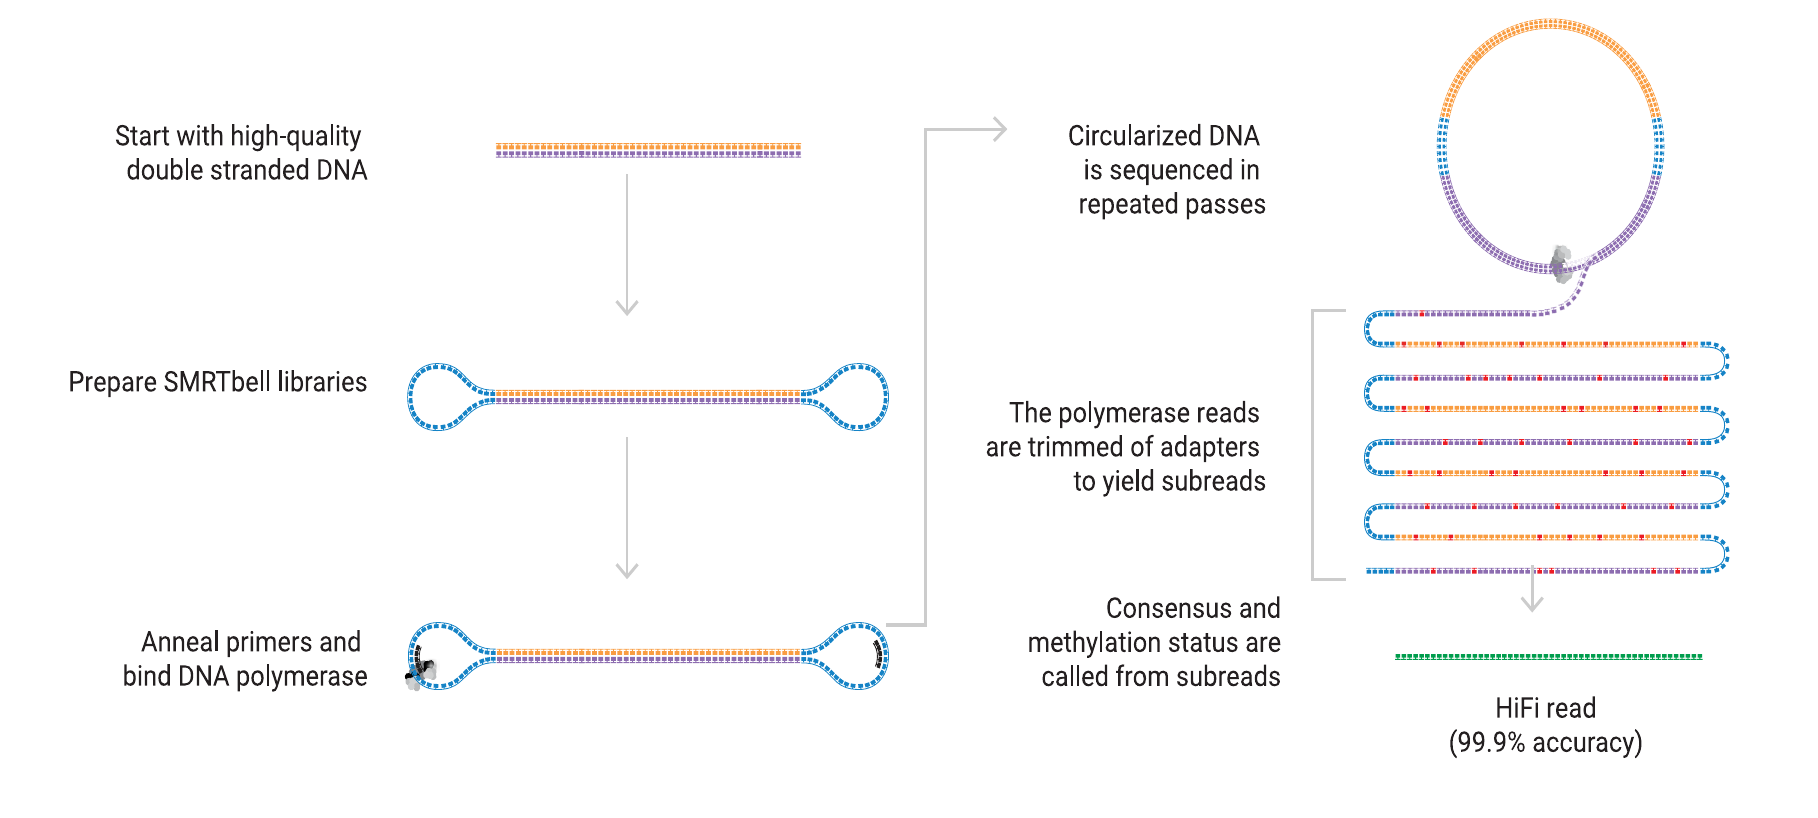
\includegraphics[width=0.95\textwidth]{figures/background/hifi_pacbio.png}
		\caption{Pacific Biosciences Hi-Fi reads generations scheme. Image from PacBio website.} 
	\end{subfigure}%
	\\
	\begin{subfigure}[b]{0.95\textwidth}
		\centering
		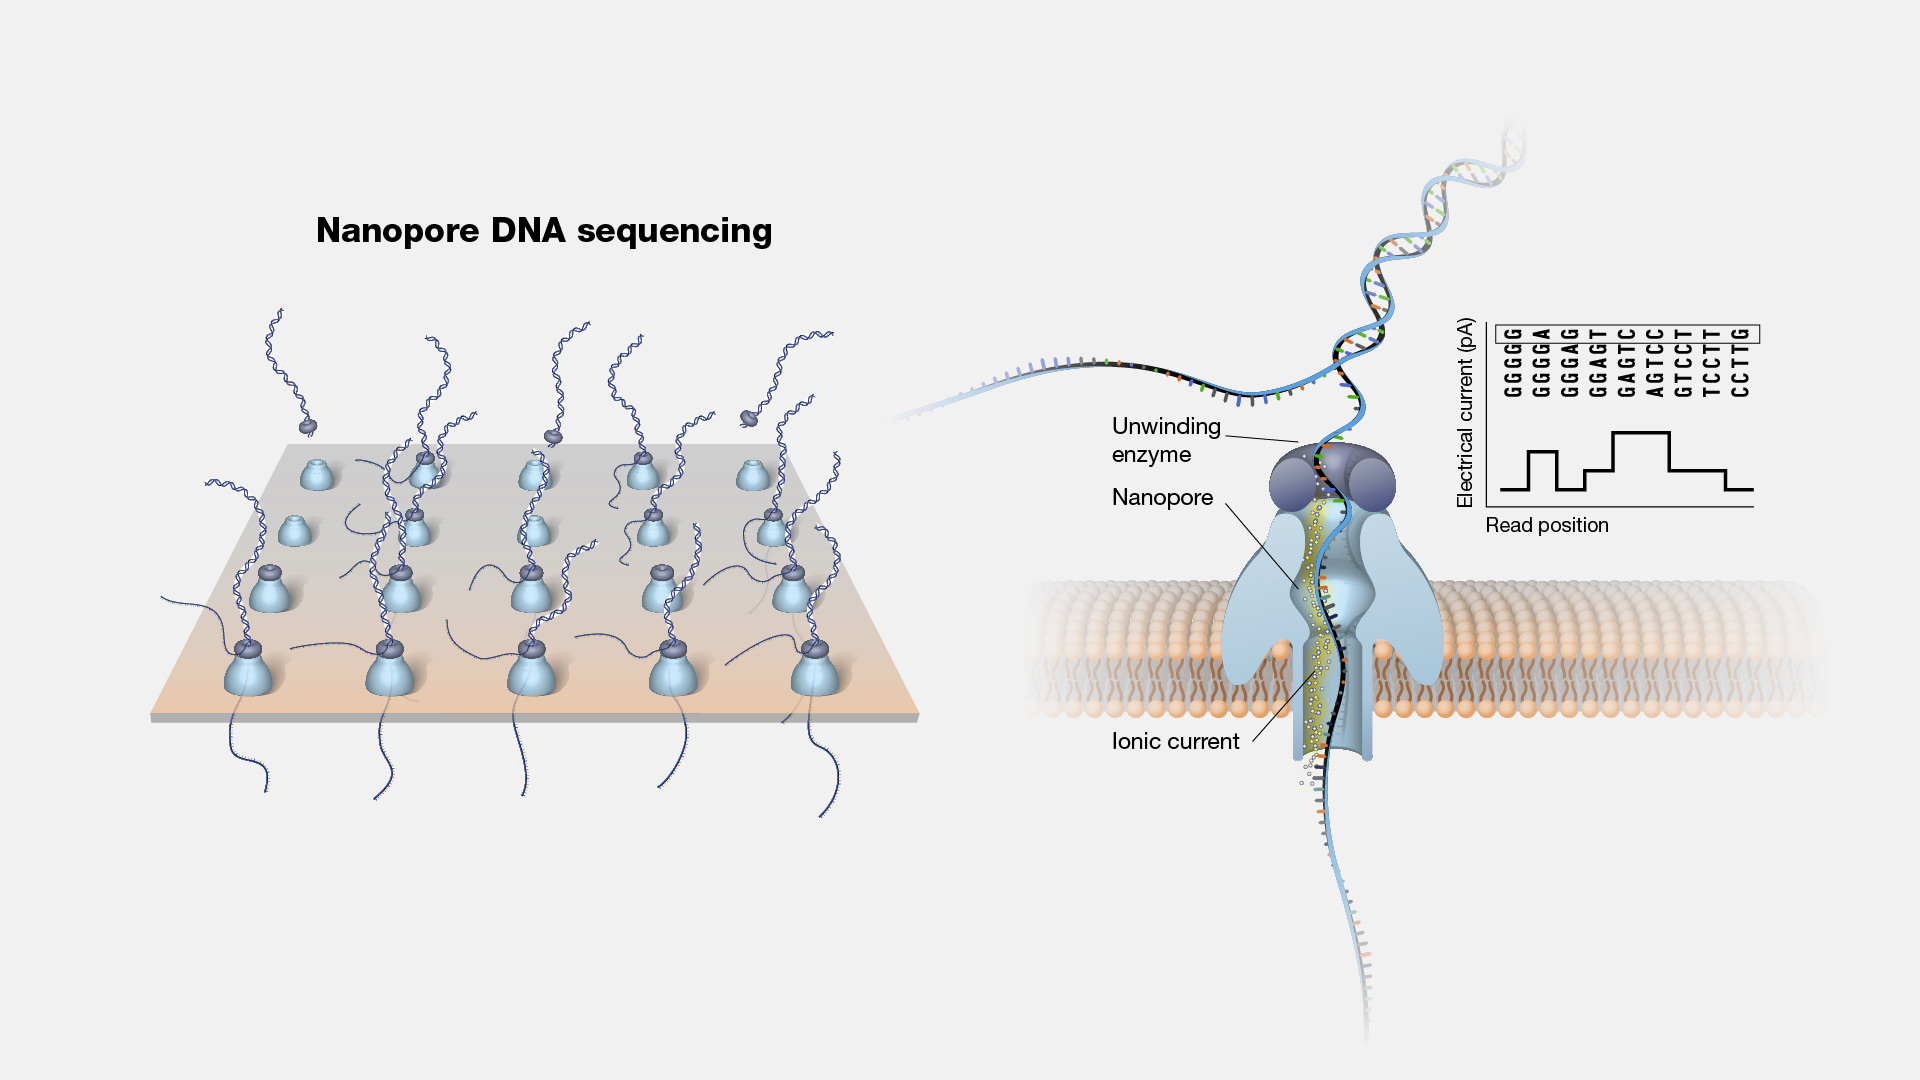
\includegraphics[width=0.95\textwidth]{figures/background/nanopore_sequencing.jpg}
		\caption{An array of pores sequences multiple molecules in parallel. A dsDNA molecule is split by the helicase enzyme and then a ssDNA sequence slowly gets through the pore for sequencing. Changes in the ionic current is used by a machine learning algorithm to infer the nucleotides of the sequence.} 
	\end{subfigure}%
	\caption{Third generation sequencing technologies.}
	\label{fig:sequencing_technologies}
\end{figure}

\section{From reads to \kmers and how to store them}
Reads are stored in formats, like FASTQ, that preserve basecalling quality information or in others, like FASTA, that retains only the actual sequence. As pair-end short-reads have different features than ultra-long reads or Hi-Fi long reads, most of the tools focus on providing applications for just one single type. In cases like genome assembly or variant calling, however, the information from different sources is combined to provide superior results. To provide high-quality genome assemblies, many consortia use Hi-Fi long reads as bases for assembly plus ultra-long reads as scaffolds to chain together the assemblies into sequences that span from telomere to telomere of a chromosome.




\section{Pangenomics, pangenomes and pangenome graphs}
\label{sec:background:pangenomics}
\subsection{Genomic diversity in populations}
The Human genome contains more than 3 billions base pairs and contains probably more than 20 thousands protein coding genes, i.e. specific parts of the DNA that serve as blueprint for proteins. The rest is non-coding, i.e. is not a gene but can serve as regulatory element, like enhancers, promoters and silencers or as other conserved, functional element.\\
DNA differs between individuals of the same population (inter-individual) and between different populations of the same species (inter-population): figure~\ref{fig:pop_diff} shows these differences for four close primates. Differences in DNA are given by having a different nucleotide at the same place (also called Single Nucleotide Polymorphism or SNP), small insertions or deletions of bases (also known as indels) and large and complex variations, up to Megabases, (also called Structural Variations, or SVs) that can produce different counts of copies or different ordering of a same region. \\
On average, each human carries around 10 thousands amino-acid altering mutations, 300-400 gene disruption events (like stop, splice and indels) affecting 200-300 genes and is heterozygous at 50-100 mutations associated with an inherited disorder~\cite{genome_diversity_quintana}. This is due genomic variability, that is assessed at
Finally, even when close species share a large portion of genetic material, structural changes that rearrange the same material in different order or invert it, contribute to meaningful changes. In figure~\ref{fig:chromosome_diff} it is shown how the chromosome 7 and 16 of some primates, even if very similar, differs in terms of organization. These large structure rearrangements are thus fundamental to understand the biology of organisms.
It is 
This is because the variation in DNA is produced by two main mechanisms: mutations and recombination. 

Moreover, genetic diversity is driven by two main factors: genetic drift and natural selection. Genomic duplication followed by adaptive mutation is considered one of the primary forces for evolution of new function
\begin{figure}[h!]
	\centering
	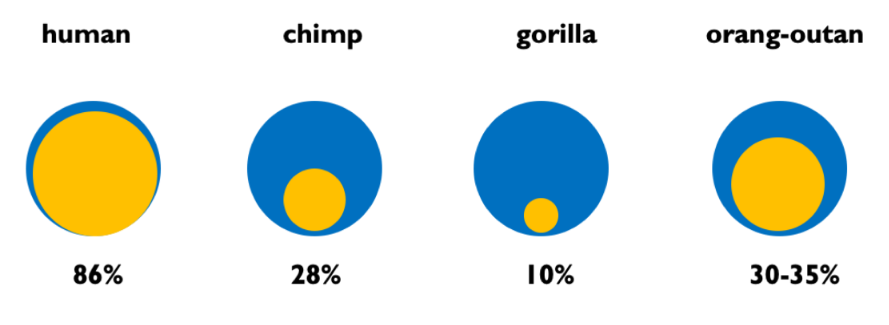
\includegraphics[width=.8\linewidth]{figures/background/pop_diff.png}
	\caption[Inter-individual and inter-population variation for 4 primate species.]{Share of inter-individual (yellow) and inter-population (blue) diversity for four different primates. While for humans the  majority of the diversity is within populations, for other primates it is between populations. This shows how Humans are more mixed than other primates. Percentage shows the inter-individual variation share~\cite{genome_diversity_quintana}.}
	\label{fig:pop_diff}
\end{figure}

\begin{figure}[h!]
	\centering
	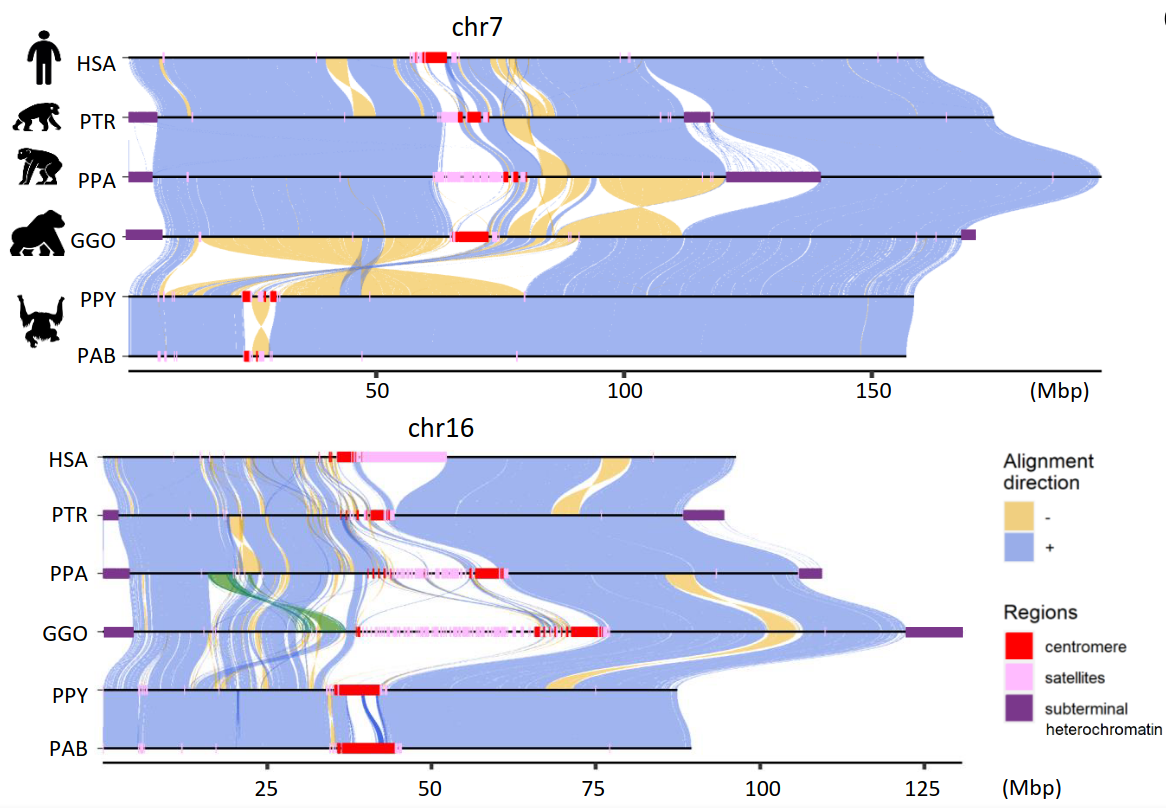
\includegraphics[width=.95\linewidth]{figures/background/genome_diff.png}
	\caption[Genomic difference in chromosome 7 and 16 of 5 primate species.]{A comparative ape alignment of human (HSA) chromosomes 7 and 16 with chimpanzee (PTR), bonobo (PPA), gorilla (GGO),Bornean and Sumatran orangutans (PPY and PAB). The image on the top shows most of the chromosome 7 is conserved except for large inversions happening between the species. The image below shows complex inversions in chromosome 16. Image taken from 'Complete sequencing of ape genomes'~\cite{ape_genomes}.}
	\label{fig:chromosome_diff}
\end{figure}

\begin{figure}[h!]
	\centering
	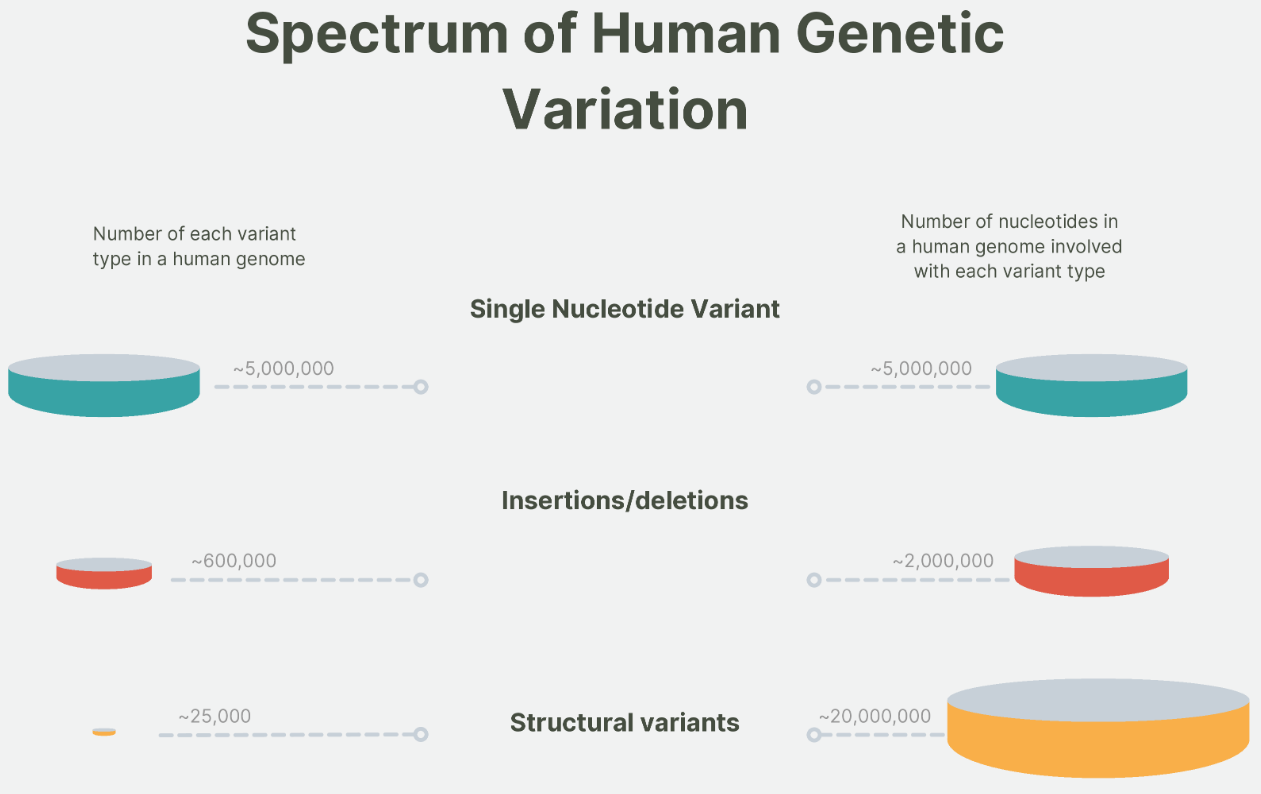
\includegraphics[width=.95\linewidth]{figures/background/spectrum_var.png}
	\caption[Spectrum of Human Genetic Variation.]{Spectrum of Human Genetic Variation. While SNPs are the most common variation Event, their impact in the total amount of bases in a genome is ~4 times smaller than the one of Structural Variations, that are 200 times less. Image produced form Evan Eichler slides that are not public.}
	\label{fig:variation_spectrum}
\end{figure}

\subsection{The premisis for human pangenomics}
\large{\textbf{A LINEAR REFERENCE FOR ALL GENOMIC ANALYSES}}\\
Since the beginning of genomics, all analysis based on sequencing data depended upon the use of a single linear reference genome, i.e. the best assembled genome available for a species, to extract useful information from the DNA. We now know that this approach is suboptimal in a wide range of applications as a lot of genetic material of the species cannot be present in a single linear refererence: this is valid for eukariotes and even more for bacteria.  
\huge{\textbf{A SEQUENCING REVOLUTION}}\\
Right now we are witnessing a real revolution in the sequencing. As the price is significantly lowering, also thanks to competition of new companies entering the market, new scientific discoveries and technological advances are leading to a remarkable increase of quality, in term of per-base error rate, and throughput. This means than right now we dispose of a rich wealth of high quality sequencing information to produce hundreds or thousands of new first grade assemblies.

\huge{\textbf{A QUALITY REVOLUTION}}
This limitation at the beginning was not solvable due to the scarcity of high quality assembled genomes as the technologies of sequencing and computational tools were not mature enough. For example, the Human Genome Project took 13 years to produce its result~\cite{humangenomeproject} and the absence of long reads with decent error rate made it impossible to automatically resolve repetitive regions like telomers and centromeres~\cite{human-pangenomics-era}, producing a reference only $92\%$ complete~\cite{t2t}. This problem was only solved in 2022~\cite{t2t}. At the same time, many consortia are producing increasingly more genomes to a level comparable to the T2T consortium. For example, the HPRC, i.e. the Human Pangenome Reference Consortium released 47 new human genomes (92 haplotypes) in 2021 and has recently released other 153 genomes to a total of 400 haplotypes. The ability to produce such high quality data for human genomes is the main driver of the \\
Right now we are witnessing a real revolution in the sequencing. As the price is significantly lowering, also thanks to competition of new companies entering the market, new scientific discoveries and technological advances are leading to a remarkable increase of quality, in term of per-base error rate, and throughput. This means than right now we dispose of a rich wealth of high quality sequencing information to produce hundreds or thousands of new first grade assemblies.
This progress lead to a shift in paradigm with increasing effort from the scientific community to propose new methods to analyse one or multiple genomes: not anymore by comparing it against a single reference sequence but against a comprehensive representation of the species. \\
This novel way to overcome the limits of "linear genomic" and consider all the variation in a single species is called pangenomics. \\
Various efforts are being made on producing reference pangenomes of yeasts, bacterias, plants and animals, including humans. In order to do so, new tools to construct and then analyse and use such representations are being developed. 
It is important here to notice, as it will be stressed in the next sections and chapters, that construction is just the first step and that is very important to understand and work on which are the operations that can be succesfully performed by these representations. \\

\subsection{Pangenomics}
\subsubsection{Pangenomes}
\subsubsection{Pangenome Graphs}

\section{Graphs}

\subsection{De Bruijn Graphs}
\subsubsection{Colored and Compacted De Bruijn Graphs}
\subsection{Variation Graphs}
\section{Outline}
\section{Pangenomics: motivation}

    
\chapter{Pushing the limit of \pangenome construction methods}
\label{sec:pushing}
In this first chapter I present and discuss two projects in which I have pushed the current limit of \pangenome constructing methods to provide useful insight of their features, of their relative advantages and of the improved capabilities compared to current genomic approaches.\\ In the first one I have analyzed the current state of the art methods available at the moment and stress-tested them by also generating what was, to the best of my knowledge, the largest human \pangenome produced at the time. \\ The second one is the generation of a yeast \pangenome reference for the species \emph{Lodderomyces elongisporus}, with some of the tools used in the aforementioned work, to demonstrate how pan-genomes are a superior representation to investigate cross-chromosomal rearrangements compared to the linear reference used by commonly used genomic tools. In order to best capture this large rearrangement between three chromosomes, I had to modify and customize one of the most used variation graph pangenome construction pipeline and compared to other two graphs. Here I present the challenges faced, discuss which data structure to use to achieve biological correctness, genome variation resolution, scalability or downstram application usability and show how a \pangenome enables improved analysis of inter-chromosome rearrangements.

\section{Motivation}
The paper that follows this section originates from a discussion early in my PhD journey on which were the best tools suited for large cohort \pangenome construction, specifically for large 
Eukaryote genomes, like primates. As pointed out in the introduction, there is no one-fits-all solution and most of the tools, at the time of the analysis, were freshly released or distributed under development. It was therefore important for the community of developers and users of such new tools and models to understand the limitations and the potential of the new pan-genomic methods.\\
In order to perform a thorough assessment of the best available methods, we tried to mimic the conditions that they could face in the near future. We therefore decided to test on the largest collection of high quality human data as it is paramount to understand how pangenomes can be used and adapted to be the platform of future large genomic studies.\\
As introduced in section~\ref{sec:background_pangenomics}, there are multiple ways of representing a group of genomes to be analyzed or used jointly. One that took traction in the last few years has been graphs. Graphs can represent the sequences as labels of nodes, relationship between them (adjacency or overlap) as edges and infer difference in the genomes as different set of nodes in them.\\
We specifically focused our attention on the most used graph models: variation graphs and De Bruijn Graphs. In variation graph edges represent adjacencies, i.e the genome is spelled by a walk on nodes connected by an edge. In De Bruijn Graphs they represent overlaps, i.e. the suffix of a node is the prefix of the next node connected to it: this implies that edges can exists between nodes that are not adjacent in the genome. As discussed in the next sessions, this distinction implies several differences in how these graphs can be used for downstream analysis. \\ 
In this article, we surveyed the the methods and tools that build such graphs, then tested them on different dataset sizes and permutations, and finally analyzed the resulting representation's features. The outcome is a small guide on which are the best applications for each of these tools and an analysis of how they represent variations in genomes. \\
%The work we performed was intended for publication, but, to the best of my knowledge, the manuscript has never been put in production.

\author
{
	Francesco Andreace
	\and
	Pierre Lechat
	\and
	Yoann Dufresne
	\and
	Rayan Chikhi
}
\title{Comparing methods for constructing and representing human pangenome graphs}

\metadata
{
	Published in \emph{Genome Biology},
	November~2023,
	volume~24,
	issue~1,
	article number 274.
	\doi{10.1186/s13059-023-03098-2}.
}
\maketitle
\label{pap:first}

\begin{abstract}
	\textbf{Background:} As a single reference genome cannot possibly represent all the variation present across human individuals, pangenome graphs have been introduced to incorporate population diversity within a wide range of genomic analyses. Several data structures have been proposed for representing collections of genomes as pangenomes, in particular graphs. \\
	\noindent \textbf{Results:} In this work we collect all publicly available high-quality human haplotypes and construct the largest human pangenome graphs to date, incorporating 52 individuals in addition to two synthetic references (CHM13 and GRCh38). We build variation graphs and de Bruijn graphs of this collection using five of the state-of-the-art tools: \bifrost, \mdbg, \minigraph, \mcactus and \pggb. We examine differences in the way each of these tools represents variations between input sequences, both in terms of overall graph structure and representation of specific genetic loci. \\
	\noindent \textbf{Conclusion:} This work sheds light on key differences between pangenome graph representations, informing end-users on how to select the most appropriate graph type for their application.
\end{abstract}

\startcontents[chapters]
\printcontents[chapters]{}{1}{\section*{\contentsname}}

\section{Introduction}
In recent years, the majority of studies on human genetics have been conducted on the basis of comparing new samples against a single, standard reference sequence. This reference sequence is a linear succession of nucleotides that acts as a blueprint of the human genome. It is routinely used to align raw sequencing data to it in order to find variations between genomes, e.g. single-nucleotide polymorphisms (SNPs), insertions or deletions (indels). It also is the backbone of the UCSC Genome Browser~\cite{ucsc} which enables inspection of genomic and epigenomic features. Despite updates that have improved the quality of the human reference sequence in the last two decades, its linear form severely limits the ability to capture population genetic diversity. For instance the locations of frequently observed structural variations cannot be easily integrated into a linear reference. To see this, consider the difficulty of designing a suitable coordinate system in the presence of (possibly nested) structural variants. Having a single genome as reference sequence also introduces an observational bias towards the chosen alleles that were integrated into that sequence, negatively impacting many primary analyses such as reads mapping, variant calling, genotyping and haplotype phasing. As a result our ability to precisely characterize structural variants, SNPs and small indels is limited \cite{vg,computational_pangenomics,giraffe}. The GRCh38 human reference genome is estimated to miss up to 10\% of our species genetic information \mbox{\cite{human-pangenomics-era}}.

Improvements in sequencing data quality and length, as well as  genome assembly methods, are providing a fast expanding collection of haplotype-resolved human genome assemblies. If adequately combined together, these high-quality individual genomes may offer an powerful alternative to the linear reference. There now is an active line of research on pangenomes, i.e. data structures that represent a collection of genomic sequences to be analyzed jointly or to form a reference \cite{computational_pangenomics,hpp}. 

Pangenome-based approaches have been shown to improve biological analyses. Pangenomes are at the basis of bioinformatics tools that perform high-quality short read mapping \mbox{\cite{giraffe}}, genotyping of SNPs, indels and SVs \mbox{\cite{pangenie}}, RNA-seq mapping \mbox{\cite{hdpr}}; de novo variant calling \mbox{\cite{vg}}; to store, compress and retrieve high quality genomes \mbox{\cite{gbz}}; to condensate all the information from a high number of genomes to then visualize specific regions or perform ad-hoc analysis, particularly on complex loci, SVs and tandem repeats \mbox{\cite{hdpr}}.
These results pave the way for new applications, e.g. genome-wide association studies, where more precise identification of variants can improve the scope of genetic studies in aging, human diseases, and cancer~\cite{computational_pangenomics, hpp}.

Several pangenomic data structures have been proposed: multiple sequence alignments, de Bruijn graphs, cyclic and acyclic variation graphs, and haplotype-centric models that use the Burrows-Wheeler transform ~\cite{computational_pangenomics}. Each of these approaches aim to represent a collection of genomic sequences in an efficient way, to store, visualize, and retrieve differences of interest between the considered genomes. 
Graph-based pangenome data structures, such as the de Bruijn graph and the variation graph, appear so far to be the most advanced in their ability to handle large amounts of input data. They are capable of representing tens to hundreds of human haplotypes simultaneously. Variations graphs use a sequence graph and a list of paths to store input haplotypes, while de Bruijn graphs store all haplotype \kmers annotated by their haplotype(s) of origin. 
Scaling pangenome graph data structures to store hundreds of genomes is a challenge that requires significant computational resources and engineering efforts. Many software tools have been created, here we briefly describe major ones.
Pantools~\cite{pantools} and Bifrost~\cite{bifrost} are two methods that have been developed to generate pangenomes for analysis on large collections of genomes, mostly for applications in phylogenetics and bacterial genomics. The PanGenome Graph Builder (\pggb)~\cite{pggb}, \mcactus and \twopaco~\cite{twopaco} are methods for building general-purpose pangenome graphs. \minigraph~\cite{minigraph} builds a particular type of pangenome graph by aligning sequences in an iterative way to a reference template. Minimizer-space de Bruijn graphs (\mdbg)~\cite{mdbg} are variants of de Bruijn graphs that can efficiently represent very large collections of bacterial pangenomes (e.g. 600,000 bacteria).  \mbox{\vg}~\mbox{\cite{vg}} builds variation graphs from a reference sequence and a variant calling file (vcf) that contains a list of variations from it.
Many human pangenomes have been generated, e.g. using Pantools~\cite{pantools} (7 genomes),  \minigraph~\cite{minigraph} (94 haplotypes), \mcactus~\cite{cactus,mcactus} and \pggb~\cite{hdpr} (94 single chromosomes), and \twopaco~\cite{twopaco} (100 simulated genomes). Lastly, a draft version of a human reference pangenome constructed using \pggb\ and the \mcactus pipeline has appeared in a very recent article from the Human Pangenome Reference Consortium~\cite{hdpr}.
These pangenomes are still limited by some factors: at the present moment, the number of high-quality haplotype assemblies is still low, even if it is expected to grow in the future; the vcf files containing variation are limited in term of bias, type of variation or number of samples; the population representation, even if opened up in recent years to more ethnicities, is still affected by sampling bias.

\section{Results}
In this article we provide a comprehensive view of whole-genome human pangenomics through the lens of five methods that each implement a different graph data structure: \mbox{\bifrost}, \mbox{\mdbg}, \mbox{\minigraph}, \mbox{\mcactus} and \mbox{\pggb}. We examine several features of pangenome graphs, in particular their scalability and how they represent genetic diversity. To this end we collected all publicly available high-quality human haplotypes and attempted to construct pangenomes of various complexity with each selected tool.
Although \mbox{\vg} has been widely used at the basis of relevant pangenome-based discoveries, for example on fast and accurate short read mapping \mbox{\cite{giraffe}}, we decided to not consider it in our analysis for two main reasons: the bias introduced by the reference sequence that is used as the backbone of the graph (and associated to the vcf) together with the limited capacity of this method to integrate structural variations from many genomes. We believe both aspects are drivers of the use of pangenome graphs.
\begin{figure}[htp]
	\centering
	\includegraphics[width=0.95\textwidth]{figures/paperI/scheme.jpg}
	\caption[The complete human pangenome construction scheme and visualization.]{\textbf{The complete pangenome construction scheme and visualization.} \textbf{A}, The overall workflow, using 5 different tools on 3 different datasets; \textbf{B}, complete 104 haplotypes variation graph built by \minigraph; \textbf{C}, focus on part of HLA (MHC) region in chromosome 6 from panel B; \textbf{D}, focus on DRB1-5 locus of HLA from panel C; \textbf{E}, complete 10 haplotypes variation graph built with \pggb; \textbf{F}, 10 haplotypes variation graph built with \mcactus; \textbf{G}, 104 haplotypes pangenome \mdbg; \textbf{H}, 10 haplotypes \bifrost \dbg. All graphs except those produced by \minigraph have been simplified using gfatools and rendered using \bandage. VG is for variation graph.}
	\label{fig:figure1}
\end{figure}


\subsection*{\textbf{Scalability and characteristics of pangenome graph construction tools \label{sec:results}}}
\label{sec:scalablility}
We ran the above five tools on three datasets consisting of 2, 10, and 104 human haplotypes respectively (Table~\mbox{\ref{tab:datasets}}). We compared the computational performance of construction algorithms as well as characteristics of the produced pangenome graphs.
The goal is to assess the ability of each method to scale to data available in the near future, i.e. thousands or even millions of human genomes~\cite{human-pangenomics-era}. \\

The performance of each tool is evaluated in terms of running 

, peak memory, disk space required by the output data structure (graph and annotations). We also compared the number of nodes, edges and connected components as indicators of the complexity of the graph. Results are displayed in Table \ref{tab:computational_metrics}. 

In terms of running time, \mdbg is two orders of magnitude faster than other tools on all considered datasets, taking around two minutes on the H2 dataset and half an hour on H104.
\bifrost is the second fastest on H104 (18 hours), and \minigraph is the second fastest on H2 (8 minutes). \mcactus takes one order of magnitude more time than \minigraph. We could not obtain graphs for \pggb and \mcactus on H104 as for the first execution did not finish after 2 weeks and the second returns an error. 

In terms of memory usage, \mdbg consistently uses less than half the memory of other tools (31 GB on H104), followed by \minigraph (61 GB on H104). On H2 all tools used between 8 and 66 GB of memory.

All tools used reasonable disk space to store the resulting graph, $\leq 12$ GB for H10 and $\leq 38$ GB for H104. Although \mcactus and \pggb retain all variations and are the only two tools able to reconstruct the input haplotypes directly from the graph, they are the second and third most efficient in term of disk space (for \mcactus, 3.6 GB on H2 and 7 GB on H10). 
While \bifrost and \minigraph perform all computation in memory, \pggb, \mcactus, and \mdbg store intermediate files on disk, taking comparable space to the input size (up to 3x for \mcactus).  \\

\subsection*{\textbf{Different tools yield different pangenome graphs topologies}}
Graph metrics such as the number of nodes, edges and connected components provide useful insights on the level of detail of the represented variations and on the complexity and accessibility of the information inside the pangenome.

The number of graph nodes varies between 17,000 and 11 millions for the H2 dataset across all tools. In all cases, the number of nodes is at least 3 orders of magnitude smaller than the number of bases in the haplotypes, indicating that pangenome graphs are effective at compressing linear parts of the haplotypes.
Tools which discard variations (\minigraph and \mdbg) yield in the order of $10^4$--$10^5$ nodes across all datasets, while tools which retain all variation (\bifrost, \mcactus and \pggb) yield in the order of $10^6$--$10^7$ nodes. In all cases going from the H10 dataset to the H104 dataset increases the number of nodes by 5x, indicating that graph complexity grows sublinearly with the number of added haplotypes.

The number of connected components varies between 2 and 1402 across all methods and datasets, and the number of large components (i.e. those with more than 1\% of total base pairs) varies between 1 and 30. 
If chromosomes were separated perfectly, pangenome graphs should contain exactly 24 connected components (one per nuclear chromosome, excluding mitochondria). \minigraph produces 24 large connected components as the number of chromosomes in the reference CHM13 v2.0 (25 including mitochondria).
\bifrost and \mcactus yield graphs with less than 25 connected components  while \mdbg and \pggb have more than 25.
In the \bifrost \dbg, the vast majority of sequences ($>$99.99\%) are in a single giant component, as chromosomes are joined because they share common \kmers. In \mdbg such joining does not occur on dataset H2, which has 24 large enough components (each containing $>$ 1\% of bases), possibly due to the absence of long and similar enough regions between chromosomes. 
\minigraph does not map any mitochondrial sequence from the input haplotypes to the reference, while they do get included into \mcactus graphs.

Even if it is common practice to analyze pangenomes chromosome by chromosome~\cite{hdpr,mcactus}, in this analysis we purposely used entire genomes as input instead. This was done for two reasons: i) to highlight the scalability of the tools, and ii) because separating chromosomes prevents the identification of inter-chromosomal inversions, translocations, and transposable elements, even if most of the generated inter-chromosomal events are probably alignment artifacts.
The effects of this choice can be seen in the \pggb and the \mcactus H10 variation graphs of Figure~\ref{fig:figure1}. In the \pggb graph 19 chromosomes are linked into a single giant component, while chromosomes 17, 18, 20, X, and Y are in other large components. This giant component consists of 25 M nodes that contain  83\% of the total basepairs. The remaining 859 components represent only 4.7\% of the total bases due to small sequences in the input haplotypes. 
In the \mcactus graph all chromosomes are linked into a single giant component except chromosome 18 that is in a separate component, and the sexual chromosomes (X and Y) that are connected together into another component.

\begin{table}
	\centering
	\caption[Computational metrics comparison between pangenome building tools.]{Time, memory, final disk space, nodes, edges, total connected components and connected components with more than 1\% of base pairs comparison of \bifrost, \mdbg, \pggb, \minigraph and \mcactus for different number of haplotypes in input. \mcactus times include the \minigraph graph construction step. \pggb was not able to complete its execution on the largest dataset in more than 2 weeks thus it is not considered. \mcactus failed to compute the 104 HAP dataset.}
	\resizebox{\textwidth}{!}{
		\begin{tabular}{|c c c c c c c|} 
			\hline
			Haplotypes & Metric &    \bifrost & \pggb & \minigraph & \mcactus & \mdbg\\
			\hline \hline
			\multirow{7}{*}{2}  &  time  (hh:mm:ss)  & 1:21:25  & 15:45:30 & 00:08:33 & 3:11:59 & 00:02:38\\
			\cline{2-7}
			& memory (GB)  & 53 & 24 & 38 & 66 & 8 \\
			\cline{2-7}
			& disk space (GB) &  4.8 & 4.3 & 2.9 & 3.6 & 4.4\\
			\cline{2-7}
			& nodes   & 9,482 k   &  8,492 k & 34 k & 10,851 k & 17 k\\
			\cline{2-7}
			& edges   & 13,108 k  & 11,503 k &  48 k & 14,702 k & 23 k\\
			\cline{2-7}
			& conn comp  & 2 & 1402 & 25 & 4 & 174\\
			\cline{2-7}
			& conn comp $>$ 1\% bp & 1 & 30 & 24 & 4 & 24\\
			
			\hline\hline
			\multirow{7}{*}{10}  & time (hh:mm:ss) &   2:27:29  &  117:08:09 & 2:03:29  & 15:57:05 & 00:05:46\\
			\cline{2-7}
			& memory (GB) & 102  & 71 & 49 & 154 & 18\\
			\cline{2-7}
			& disk space (GB) &  12  & 7.6 &  2.9 & 7 & 9.7\\
			\cline{2-7}
			&  nodes   & 27,468 k   & 29,315 k &  133 k & 37,767 k & 67 k\\
			\cline{2-7}
			&  edges  & 37,584 k  & 40,282 k &  190 k & 51,595 k & 93 k\\
			\cline{2-7}
			& conn comp   &  3   & 864 & 25 & 3 & 40\\
			\cline{2-7}
			& conn comp $>$ 1\% bp &   1   & 5 &  24 & 3 & 1\\
			
			\hline\hline
			\multirow{7}{*}{104}  & time (hh:mm:ss)  &  18:38:28   &  ---  & 46:22:00  & --- & 00:31:38\\
			\cline{2-7}
			& memory (GB) & 122 &  ---  &  61 & --- & 39\\
			\cline{2-7}
			& disk space (GB)  &  29.4  & ---  &  3.2 & --- & 38\\
			\cline{2-7}
			&  nodes  & 106,339 k  &  ---  & 632 k & --- & 270 k\\
			\cline{2-7}
			&  edges  & 293,839 k  &  ---    & 912 k & --- & 396 k\\
			\cline{2-7}
			& conn comp   &  17  &   ---  & 25  & --- & 1097\\
			\cline{2-7}
			& conn comp $>$ 1\% bp &  1   & --- & 24 & --- & 1\\
			
			\hline
	\end{tabular}}
	\label{tab:computational_metrics}
\end{table}

\subsection*{\textbf{Interpretation of variation in pangenome graphs: focus on two HLA loci}}
\label{sec:loci}
The ability to detect and annotate variations among input haplotypes defines the scope of each pangenome graph construction method. Previous work~\cite{chin} recommends to build graphs on a specific loci rather than the entire genome for the purpose of i) identifying genomic diversity and ii) mapping raw reads to divergent regions, specifically difficult-to-map repeats. Here we evaluate how pangenomes built from entire haplotypes represent specific biologically relevant loci.

\paragraph{\textbf{\textup{Extraction of HLA-E and a complex HLA region from complete pangenome graphs}}}
We extracted from complete pangenomes the regions corresponding to two loci of the Human Leukocyte Antigen complex, also known as HLA. These regions are highly medically relevant  as they contain many disease-associated variants~\cite{HLA-nature}.
The first locus is the HLA-E gene, that is part of the nonclassical class I region genes, spanning 4,8 kbp and is relatively conserved across populations.
It has been shown to have significant association with hospitalization and ICU admission as a result of COVID-19 infection \cite{hla-e-covid}.
The second is an HLA complex region comprising the HLA-A gene, part of the classical, highly polymorphic class I region. It is around 58 kbp long and contains the HLA-U, HLA-K, HLA-H, and HCG4B genes. 
We extracted these two regions from  pangenome graphs using a custom script that yields a subgraph corresponding to a given set of sequences and their variation. The script uses a different recommended method %method for each of the five types of pangenome graphs as it uses recommended tools 
for each of the pangenome graph types. In a nutshell, we extracted regions using exact coordinates when possible, and resorted to sequence-to-graph alignment otherwise (see Appendix Section "Loci extraction method" for details). 
While on variation graphs and mDBGs nearby nodes of an aligned region correspond to variations of the locus, this is not always true for standard \dbgs. Extracting accurate and complete loci representation is an unsolved challenge for \dbgs. \\

\paragraph{\textbf{\textup{HLA-E: a low complexity region}}}
Figure \ref{fig:HLA-E} shows how the different tools represent HLA-E over datasets H2, H10 and H104. As expected, \minigraph does not detect any variation, since the SNPs that characterize the region are too small to be considered in the construction steps of their algorithm. \pggb, on the contrary, has 2 SNPs in H2 and 3 in H10. \bifrost detects the same SNPs as \pggb in H2 and H10. Both of them represent the exact same variations and render the same haplotypes paths. \mbox{\mdbg} captures the heterozygosity of a large region containing the HLA-E locus as the number of samples grows. As the \mbox{\mdbg} graph is built in minimizer space, nodes represent long genomic segments (in the order of hundreds of thousand of base-pairs). In H10 and H104, the minimizer-space representations of the haplotypes are identical; however, differences in flanking regions of the graph create variations that are captured in extra nodes that are also extracted in this region. On H2, \mcactus detects 3 variations as the dataset used is different, containing the CHM13 reference and just one haplotype of HG006 (as in \minigraph), as discussed in Section "Datasets and haplotypes collection". 

Figure \ref{fig:HLA-E} also illustrates how pangenome complexity grows with the number of genomes: the \bifrost H104 subgraph has the most variation across all methods, highlighting that dBGs represent variations exhaustively in large graphs. On the other hand, \pggb has the most straightforward method for extracting subgraphs, and also represents variants exhaustively in datasets H2 and H10, but could not scale to the H104 dataset.

\begin{figure}[htp]
	\centering
	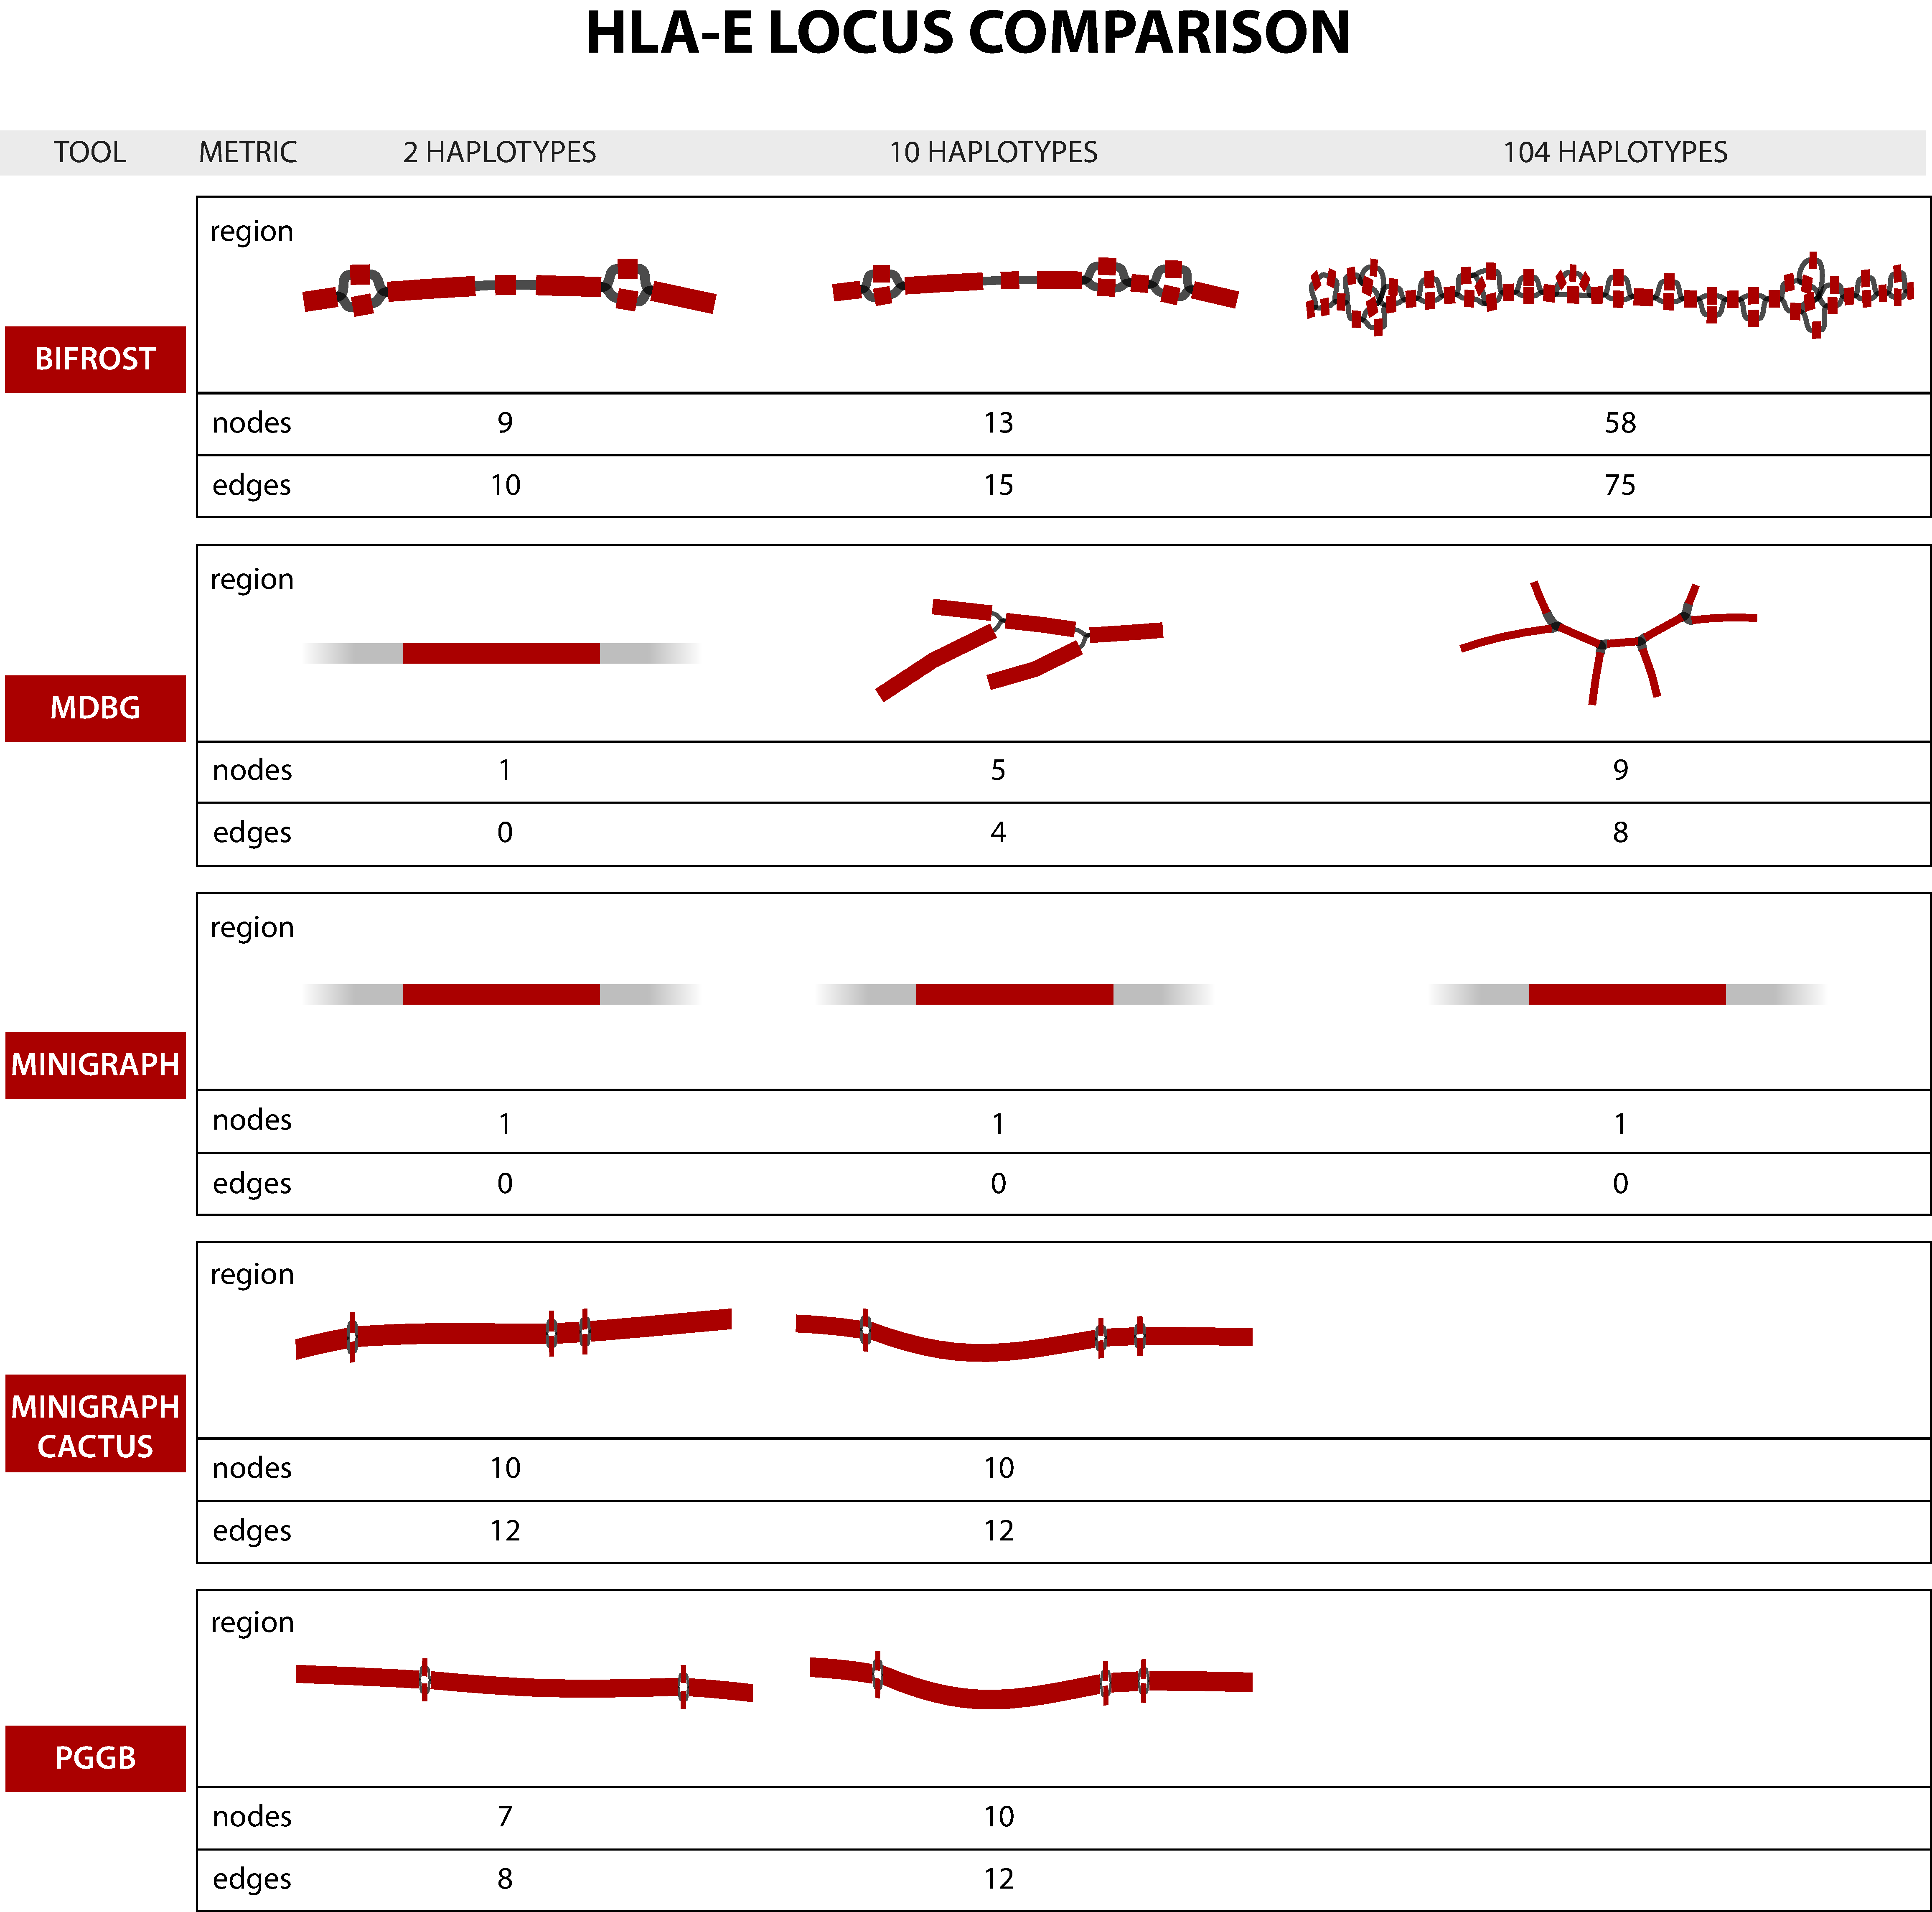
\includegraphics[width=0.95\textwidth]{figures/paperI/hla-e_corrected.pdf}
	\caption[Representations of the HLA-E locus on large human pangenomes.]{Representations of the HLA-E locus by five graph construction methods over three increasing large human pangenomes. Nodes highlighted in red contain part of the locus sequence. The numbers of nodes and edges displayed below each graph concerns the whole subgraph (both red and grey nodes). %, i.e. nodes and edges directly or indirectly attributed to the sequences that represent the locus. 
		\minigraph, on H2, H10 and H104, and \mdbg, on H2, have only a portion of one node highlighted since the 4.8k bp region is contained inside a single, long node.} 
	\label{fig:HLA-E}
\end{figure}

\paragraph{\textbf{\textup{HLA complex locus: high complexity region}}}

Figure \ref{fig:HLA-A} is the counterpart of Figure~\ref{fig:HLA-E} for the complex locus part. In this case the overall interpretability of the region is more challenging, as the number and the structure of the variations is different than in HLA-E. It is also more difficult to compare across tools. Base-level variations, e.g. SNPs, are not visually recognizable in Figure~\ref{fig:HLA-A} in the methods that retain them (i.e. \pggb, \mcactus and \bifrost) due to the large sizes of graphs.

There are notable differences in how  tools represent the variation, which is well-illustrated in the H2 dataset. While \minigraph renders H2 as a single sequence plus a large structural variant (SV) of $\approx$ 52k bp, \pggb separates it into two paths that differ by $\approx$ 54k bp in length. \bifrost represents a detailed bubble that contains many variations inside each path. In \mdbg, even extracting the complete locus is a challenge as many of the subgraph nodes were not selected by our procedure. \mcactus adds base level divergences between haplotypes on top of \minigraph SV graph.

These differences between representations are further accentuated in the H10 dataset. For it, \pggb tends to separate the haplotypes into different paths, \bifrost renders consistently the same compacted representation and \minigraph neglects most of the small differences but is able to display accurately the general picture, and \mcactus, as in H2, adds small variations on top of \minigraph structure. 


\begin{figure}[htp]
	\centering
	\includegraphics[width=0.95\textwidth]{figures/paperI/hla-a_corrected.pdf}
	\caption[Representations of the HLA-A locus on large human pangenomes.]{Representations of the complex HLA region by five graph construction methods over three increasing large human pangenomes. 
		See caption of Fig.~\ref{fig:HLA-E} for details. 
		%.Nodes highlighted in red are the ones that contain part of the locus sequence. The number of nodes and edges displayed represent the ones directly or indirectly attributed to the sequences that represent the locus.
	}
	\label{fig:HLA-A}
\end{figure}

\subsection*{\textbf{Uncovering characteristics of graphical pangenome tools}}
\label{sec:uncovering}
The data structures generated by pangenome building tools are expected to facilitate comparisons between the input genomes. In addition pangenome graphs should be stored in such a way to be easily used by downstream applications.
We identify 8 important features for pangenome graph construction tools: i) stability, ii) editability, iii) accessibility by downstream applications, iv) haplotype compression performance v) ease of visualization, vi) quality of metadata and annotation. Two other but important features, scalability and interpretability of produced graphs, were already discussed in Sections "Scalability and characteristics of pangenome graph construction tools" and "Interpretation of variation in pangenome graphs: focus on two HLA loci". %\ref{sec:scalablility} and \ref{sec:loci}. 
Table \ref{tab:tools_consideration} summarizes some of the following considerations on the relative strength of the tools.

\paragraph{\textbf{\textup{Editability and dynamic updates}}}
%\noindent\textbf{EDITABILITY AND DYNAMIC UPDATES} 
As more high quality assemblies will be generated in the near future, haplotypes may be added to a pangenome, or replaced by improved versions. Updating an existing data structure instead of rebuilding it from scratch is both computationally and energetically efficient. 
However, many succinct data structures currently used in pangenome representation are static, i.e. cannot be updated. %Current
Some methods allow a restricted set of editing operations.
\minigraph allows to add new haplotypes on top of an already built graph. \bifrost provides C++ APIs to add or remove \mbox{(sub-)sequences}, \kmers and colors from the ccdBG.
\pggb, using \odgi~\cite{odgi}, allows specific operations that delete and modify nodes and edges and add and modify paths through the graph. As \mcactus can be opened with \odgi, it supports the same operations as \pggb. 
The current \mdbg implementation uses a dynamic hash table, but does not expose an interface that supports updates.

\paragraph{\textbf{\textup{Stability}}}
%\noindent\textbf{STABILITY} 
Counter-intuitively, a pangenome graph construction tool may in some cases generate different outputs when executed multiple times with the same haplotypes as input. This \emph{unstability} could be due to a permutation in the order of the sequences given as input, or non-determinism in the construction algorithm.
Yet in order to facilitate the reproducibility of results, pangenome building tools should generate an unchanged output from the same set of input sequences, independently of the particular run or the order in which these are given.
We performed two tests to evaluate tool stability: i) we run the tools 3 times using as input the same H10 dataset and ii) we run the tools twice on shuffled input sequences, i.e. changing the order of the haplotypes of H10. 

\bifrost and \mdbg constructed exactly the same pangenome on every test, as by definition, de Bruijn graphs are stable.
\minigraph generates identical graphs on identical inputs, but generates slightly different graphs when the input is permuted. Indeed the construction algorithm of \minigraph is order-sensitive as it augments the existing graph structure by aligning the next given haplotype to it and adding divergent sequences. 
\mcactus generates slightly different graphs on identical input. 
\pggb\ generated slightly different graphs while maintaining the same haplotype sequences in the paths. The overall representation of the input genomes is therefore preserved, while the topology of the variation graph varies. The first two of the three phases of the \pggb pipeline (all-vs-all alignment and graph imputation) produce the same result on different runs with the same input but differences arise when the order of the input haplotypes changes. Most of the differences in the graph topology are thus due to the final smoothing steps.

\paragraph{\textbf{\textup{Accessibility by downstream applications}}}
% \noindent\textbf{ACCESSIBILITY BY DOWNSTREAM APPLICATION} 
\label{subs:downstream}
To facililate their adoption, pangenome representations should be easily processed by downstream analyses. 
De Bruijn graphs are challenging to analyze due to their high number of nodes, edges, and redundancy (the $k-1$-overlaps between nodes).
Though De Bruijn graph representations usually support queries of presence/absence on nodes (as in \bifrost), they lack tools able to perform more elaborate analyses such as those discussed in Section "Interpretation of variation in pangenome graphs: focus on two HLA loci", e.g. incorporating haplotype information at the \kmer level. 
On the other hand, variations graphs with paths provide more flexibility, i.e. as in \pggb and \mcactus with the \odgi visualization toolkit.
Finally in \minigraph, which considers a narrower spectrum of variants, the absence of path information prevents haplotype-level analysis; haplotypes would need to be manually mapped back to the graph. 
The choice of the pangenome building tool depends on the envisioned application. \mbox{\pggb} and \mbox{\mcactus} graphs have been shown to outperform linear references for short read mapping, genotyping and RNA sequencing mapping \mbox{\cite{hdpr}}. As these two methods  are complex pipelines based on multiple tools where parameters have been carefully set, they can be more challenging to install and run than single integrated tools. \mbox{\minigraph} alone can also be used if the focus is on structural variation instead of SNPs or small indels, and to quickly produce a pangenome graph for complex loci visualization and interpretation. The dBG-based approaches show that, for example with \mbox{\bifrost}, they retain the same base-level information as more computational-heavy variation graph approaches, but the lack of tools to use them for analysis limits their adoption.

\paragraph{\textbf{\textup{Haplotype compression}}}
%\noindent\textbf{HAPLOTYPE COMPRESSION} 
Building a graph pangenome can be seen also as a way to store, compact and retrieve the input haplotypes. As the number of new assemblies is growing faster than the data storing capacity, pangenomes can potentially help save storage space. This is highlighted by the disk space reported in Table~\ref{tab:computational_metrics}, which is consistently smaller than the sum of haplotype sizes for all methods and datasets.

In order to losslessly retrieve the input genomes from a pangenome, the  representation has to store all variations from the original haplotype sequences as paths in the graph. \pggb and \mcactus fall into this category while the other three considered tools do not store paths, or do not consider all variations, thus they are lossy.

Of note, the GBZ tool~\cite{gbz} enables graph pangenomes that store paths in the GFA file format %(the consensus file format used) 
to be stored in a lossless compressed form. It uses a Graph Burrows-Wheeler transformation to compress the graph in a more efficient way than using gzip~\cite{gbz}. Using GBZ, the pangenomes generated by \pggb and \mcactus are losslessly compressed with space gains of 3.5-5x.


\paragraph{\textbf{\textup{Ease of Visualization}}}
%\noindent\textbf{EASE OF VISUALIZATION} 
Visualizing large graphs which exceed hundreds of thousands of node is a challenge that exceeds the scope of pangenomics. The H104 pangenomes  are difficult to visualize.
Among the visualization tools considered by the Human Pangenome Reference consortium~\cite{hpp}, 
only \bandage is able to display the \minigraph or \mdbg H104 graphs, which contains a few million nodes. We reduced the number of nodes and edges of \pggb, \mcactus and \bifrost H10 graphs by collapsing isolated subgraphs representing SNPs or indels up to 10k bp (using the command \texttt{gfatools asm -b 10000 -u}). % to be able to display them. 
%Generally, general-purpose graph drawing tools able to visualize graphs with millions of nodes are needed, in particular to extract and display specific loci.

\paragraph{\textbf{\textup{Quality of Metadata and Annotation}}}
%\noindent\textbf{QUALITY OF METADATA AND ANNOTATION} 
Augmenting pangenome structures with information from other omics data would increase pangenome relevance in biological discoveries. As biobanks are rapidly growing, more data is available on regulatory regions, transcriptomics, CNVs and other medically relevant traits~\cite{100000genomes,ucla}. Pangenome data structures could leverage such information, and some of the considered tools offer basic functionality in this sense.
\bifrost provides a function to link data to graph vertices through C++ APIs. \pggb and \mcactus, using \odgi, offer annotation capabilities through insertion of paths or BED records. \minigraph and \mdbg do not offer any annotation feature. 
Specifically, in order to enhance a pangenome graph with metadata (for example with genes and regulatory regions known variants), it is desirable to maintain compatibility with methods and data formats that use a linear reference. One could conceivably project data from a graph to a reference genome to continue downstream analyses using linear coordinates. A simple method to achieve this compatibility, in our view, is to store the reference genome of interest inside the graph pangenome that supports retrieving such a reference. Variation graphs built using \mbox{\pggb or \mcactus}, due to their locally acyclical and directed construction and their use of haplotype paths, store all the coordinates needed for such a task. Haplotype paths play an important role as they avoid additional mapping to the graph, by using the \mbox{\odgi}tool to extract or inject the required information. \mbox{\minigraph} does not store haplotype paths and requires mapping sequences to the graph to restore haplotype information. On the other hand, De Bruijn graphs, using associated color data, can record the membership of k-mers to a reference sequence, yet one cannot fully reconstruct a haplotype unless k-mers positions are also stored.
\begin{table}
	\centering
	\caption[Relative strengths of five pangenome graph construction tools.]{\textbf{Relative strengths of five pangenome graph construction tools}\\
		Explanation of rows:
		1) efficacy of construction algorithm, measuring wall-clock time;
		2) degree to which variants (e.g. SNPs) are retained;
		3) ability of a tool to perform well on large datasets, both in comparison to other tools but also compared to smaller datasets;
		4) ability to modify the produced data structure to add or remove haplotypes; 
		5) property of producing the same result irrespective of perturbations, such as permutation of the input order, and repeating the same run;
		6) existence of tools (and operations) that can be applied to the resulting graphs; 
		7) whether input haplotypes information is retained by the tools, and if so, its space efficiency;
		8) whether the entire graph can be directly visualized and interpreted; 
		9) easiness of 'zooming in' a specific genomic region and interpret variants;
		10) summarizes the functionalities provided by the tools to annotate the pangenomes with genomic data;
		11) ability to share information between the graph and a linear reference.
	}
	\resizebox{\textwidth}{!}{
		\begin{tabular}{|l c c c c c|} 
			\hline
			Metric & \bifrost & \pggb & \mcactus & \minigraph & \mdbg\\
			\hline
			1) Construction speed & $\bullet\bullet\circ$ & $\bullet\circ\circ$ & $\bullet\circ\circ$ &  $\bullet\bullet\circ$ & $\bullet\bullet\bullet$\\
			\hline
			2)  Variations & $\bullet\bullet\bullet$ & $\bullet\bullet\bullet$ & $\bullet\bullet\bullet$ & $\bullet\bullet\circ$ & $\bullet\bullet\circ$\\
			\hline
			3) Scalablilty & $\bullet\bullet\bullet$ & $\bullet\circ\circ$ & $\bullet\circ\circ$ & $\bullet\bullet\circ$ & $\bullet\bullet\bullet$\\
			\hline
			4) Editability & $\bullet\bullet\bullet$ & $\bullet\bullet\circ$ & $\bullet\circ\circ$ & $\bullet\bullet\circ$ & $\bullet\circ\circ$\\
			\hline
			5) Stability & $\bullet\bullet\bullet$ & $\bullet\circ\circ$ & $\bullet\circ\circ$ & $\bullet\bullet\circ$ & $\bullet\bullet\bullet$\\
			\hline
			6) Accessibility by downstream applications & $\bullet\circ\circ$ & $\bullet\bullet\bullet$ & $\bullet\bullet\bullet$ & $\bullet\bullet\circ$ & $\bullet\circ\circ$\\
			\hline
			7) Haplotype compression performance & $\bullet\bullet\circ$ & $\bullet\bullet\bullet$ & $\bullet\bullet\bullet$ & $\bullet\circ\circ$ & $\bullet\circ\circ$\\
			\hline
			8) Ease of visualization  & $\bullet\circ\circ$ & $\bullet\bullet\circ$ & $\bullet\bullet\circ$ & $\bullet\bullet\bullet$ & $\bullet\bullet\bullet$ \\
			\hline
			9) Loci visualization and interpretability   & $\bullet\circ\circ$ & $\bullet\bullet\circ$& $\bullet\bullet\bullet$ & $\bullet\bullet\circ$  & $\bullet\circ\circ$\\
			\hline
			10) Metadata and annotation   & $\bullet\bullet\circ$ & $\bullet\bullet\bullet$ & $\bullet\bullet\circ$ & $\bullet\circ\circ$  & $\bullet\circ\circ$\\
			\hline
			11) Compatibility with a linear reference coordinates & $\bullet\circ\circ$ & $\bullet\bullet\bullet$ & $\bullet\bullet\bullet$ & $\bullet\bullet\circ$  & $\bullet\circ\circ$\\
			\hline
	\end{tabular}}
	\label{tab:tools_consideration}
\end{table}

\section{Discussion}
Five state-of-the-art pangenome graphs construction tools were compared on the representation of up to 104 human haplotypes. The approaches significantly differ in terms of speed, graph size, and representation of variations. We find that it remains computationally prohibitive to generate human pangenome graphs for hundreds of haplotypes, especially while retaining all variations. Each approach has its own set of strengths, and ultimately the choice of the method depends on the downstream application. In addition, several takeaway points emerged from our analysis.

First, our focused analysis of HLA loci revealed that de Bruijn graphs and variation graphs represent genomic variations equally well as pangenomes.  This is of particular importance as also shown by the draft human pangenome references~\mbox{\cite{hdpr}}: pangenomes are pivotal to trace complex and clinically relevant loci. While de Bruijn graphs are faster to construct, more stable, and scale better in terms of input size, the resulting graphs are challenging to interpret downstream. Variations graphs on the other hand are more practical to analyze at the expense of a less efficient construction step. Their visualization are more straightforward to interpret, mostly due to not having cycles, and provide insights into loci differences. 

Second, we can highlight two categories of pangenomic methods that have distinct application domains. \pggb, \mcactus and \bifrost store all possible variations, and keep haplotype information as paths or colors. They provide a complete picture of the set of variations in the input genomes which makes them difficult to analyze. They can be used for a large variety of genomic analysis, as shown for \mbox{\pggb} and \mbox{\mcactus}~\mbox{\cite{hdpr}}. \minigraph and \mdbg generate 'sketched' pangenome graphs that consider only large variants, ignoring smaller differences, and are more efficient to construct and visualize. They can be used for large scale characterization of variation in population, as proven for bacteria \mbox{\cite{mdbg}}.

Third, every tool possesses an exclusive set of features.
\pggb facilitates downstream analyses using the companion tool \odgi. It allows to precisely extract and browse any locus of interest. It is the only tool that generates variation graphs without a reference. It also keeps a lossless representation of the input sequences.
\minigraph generates a pangenome graph based on a reference sequence taken as a backbone. Its shines in the representation of complex structural variations, but does not include small or inter-chromosomal variations.
The pipeline \mcactus, that uses the \cactus base aligner, can be used to add small level variations on top of the \minigraph graph and to keep a lossless representation of the input sequences.
\bifrost illustrates that classical de Bruijn graphs are scalable, stable, dynamic, and store all variations. However, extracting information from them remain a challenge.
Lastly, \mdbg\ is the fastest construction method which generates an approximate representation of differences between haplotypes. As discussed in Section "Accessibility by downstream applications", these features enable different genomic analyses and downstream applications.

\section{Conclusions}
In conclusion, our results highligh the strengths and weaknesses of current pagnenome construction tools for human applications, with specific focus on how do they represent specific loci of medical relevance. We also provide insights on the features they possess and point out their best application domains.
In our view, future directions for human pangenomes building tools should focus on tackling efficiency bottlenecks, aiming to represent hundreds to thousands of haplotypes. Representations should further be lossless and represent the input haplotypes as paths in the graph. 
Such features would unlock many other applications such as lossless compression of haplotypes and cancer copy number variant analysis. 
Finally, we recognize the need for more user-friendly tools that can be used by biologists and that can translate complicated questions into  graph queries. While \odgi begins to address these questions in variation graphs, other approaches have not yet provided user-friendly interfaces. A package similar to \odgi for de Bruijn graphs would help fully realize their potential.

\section{Methods}
\subsection*{\textbf{Datasets and haplotypes collection}}
\label{sec:datasets}
In order to evaluate the state of current human pangenome representations, we sought to build a human pangenome that contains all publicly available high-quality human haplotypes. We collected from two different sources 102 different haplotypes from the genome of 51 individuals, and also used the two reference genomes, GRCh38 from the Genome Reference Consortium (GRC) \cite{grc} and CHM13 v2.0 cell line of the T2T Consortium~\cite{t2t}.
Five haplotypes correspond to Google Brain Genomics DeepConsensus \cite{deepconsensus} assembly dataset: they are hifiasm assemblies of PacBio Hi-Fi reads corrected with DeepConsensus. The average of their N50 is 37,99 Mbp. 
The remaining haplotype assemblies as well as the T2T reference are from the Human Pangenome Reference Consortium (HPRC) year-1 freeze~\cite{hpp}, and GRCh38 is from the GRC. Their average N50 is 40.3 Mbp. Since HG002 is contained in the DeepConsensus data, the HPRC HG002 haplotypes were not used.
The origin and the sex of the individuals are diverse %to aim for a 
and provide a fair representation of the diversity in human population: out of 51 total individuals, 21 are males and 30 are females and they represent 14 different ethnic groups, from US to Africa and Asia. We did not perform any additional selection, regarding sex and ethnicity, on these public datasets as our main goal was to use as many genomes as possible. However, the HPRC stated that the genomes were selected to represent genetic diversity in humans~\mbox{\cite{hdpr}}.

To evaluate the scalability of pangenome construction tools, we created three datasets of increasing size: 1) 2 haplotypes from the same individual, HG006, 2) 10 haplotypes from 5 different individuals (HG002, HG003, HG004, HG006 and HG00735) and finally 3) all of the 104 haplotypes. To test whether the order of the input sequences matters, we considered various random orderings for the 10 haplotypes in Dataset 2. Since \minigraph needs a reference sequence as fist haplotype in order to correctly build the graph, we generated specific 2 and 10 haplotypes datasets with the first haplotype replaced by the reference genome CHM13. This was applied to the \mcactus pipeline as well as it uses \minigraph variation graphs.

\begin{table}
	\centering
	\setlength{\tabcolsep}{5pt} 
	\caption[Description of the three datasets generated to test the scalability of the tools.]{\textbf{Description of the three datasets generated to test the scalability of the tools}
		\\
		Data sources: 
		$^1$ Google Brain Genomics~\cite{google-assemblies}; $^2$ Human Pangenome Reference Consortium~\cite{HPRC-haplotypes}; $^3$ 1000 Genomes Project~\cite{HPRC-haplotypes}; $^4$ Telomere to Telomere Consortium~\cite{HPRC-haplotypes}.
		\label{tab:datasets}}
	\renewcommand{\arraystretch}{1.2}
	\begin{tabular}{|c c c|}
		\hline
		\centering
		Haplotypes & Project & Bases \\
		\hline
		2 & Google$^1$ & 5.9 Gbp\\
		10 & Google, HPRC$^2$ & 30 Gbp \\
		104 & Google, HPRC, 1KG$^3$, T2T$^4$ & 313.6 Gbp \\
		\hline
	\end{tabular}
\end{table}

\subsection*{\textbf{Pangenome graph construction tools}}
\label{sec:tools}

We evaluated tools that generate graph pangenomes as variation graphs and colored compacted de Bruijn graphs. Variation graphs are generally locally acyclic while de Bruijn graphs have cycles. In variation graphs, nodes represent sequences and edges represent immediate sequence adjacency without overlap. Variation graphs are generally easier to visualize and to interpret while challenging to construct at scale and, apart from \pggb, require a reference genome. In de Bruijn graphs (\dbg), nodes are \kmers (string of length k) and edges are (k-1)-overlaps between nodes. In practice, \dbgs are represented in a compact way where all nodes along unbranching paths are compacted into \emph{unitigs}. The resulting graph is called compacted De Bruijn Graph, where nodes are unitigs and edges represent (k-1)-overlaps. 
As shown in Figure \ref{fig:figure1}, de Bruijn graphs %are easier to construct and are more standardized but 
result in large graphs that pose visualization and interpretation challenges, in particular as there is no alignment to a reference.

\begin{itemize}
	\item
	\bifrost constructs dynamic, coloured compacted de Bruijn Graphs (\emph{\ccdbg}). It first generates a standard \dbg using an efficient variant of Bloom Filters and then computes the compacted \dbg from it.
	Colors, i.e. identifiers representing the sample origin of each k-mer are added by storing an array per \kmer. A human genome \ccdbg typically consists of a single large connected component, as common \kmers are shared between chromosomes. This pangenome representation contains all the variations present in input sequences.
	
	\item
	\mdbg builds a variant of de Bruijn graphs called a minimizer-space de Bruijn Graph (\mdbg), which is efficient to construct as it only considers a small fraction of the input nucleotides. Color information is currently not supported in the implementation. Similarly to Bifrost, a \mdbg also typically represents a human genome as a single large connected component, albeit with orders of magnitude less nodes. Minimizer-space de Bruijn graphs mostly discard small variants, yet are sensitive to heterozygosity which creates branches in the graph.
	
	\item
	\minigraph constructs a directed, bidirected and acyclic variation graph iteratively by mapping new haplotypes using a combination of the minimap2 tool and the graph wavefront alignment algorithm. The first input sequence acts as a  backbone for the whole representation.
	The sample(s) of each node are stored in a rGFA output file.
	\minigraph considers only variations longer than 50 bps hence it is oblivious to isolated SNPs and small indels: even if it produces base-level alignment for contigs, the graphs are not a base-level resolution. The resulting graph is divided into connected components that correspond to the chromosomes present in the first given input genome.
	%, yet can represent large divergent regions at base-pair resolution
	\item
	\mcactus is a variation graph construction pipeline that combines \minigraph to generate a structural variations graph and \cactus base aligner to generate base-level pangenome graphs of a set of input assemblies and embg: The definition of \label has changed! Check your packages! Replacing it with the kernel definition on input line 145.ed haplotypes paths. \cactus~\cite{cactus} is a highly accurate and scalable reference-free multiple whole-genome alignment tool, that in this pipeline considers the reference sequence used by \minigraph to ensure that the resulting variation graph is acyclic. The final graph is further normalized using GFAffix\cite{gfaffix}. The pipeline allows to generate multiple graphs, one for each chromosome, or produce a single graph that includes inter-chromosomal variants.
	
	\item
	\pggb is a directed acyclic variation graph construction pipeline rather than a single tool. It calls three different tools: pairwise base-level alignment  of haplotypes using wfmash \cite{wfmash}, graph construction from the alignments with seqwish \cite{seqwish}, graph sorting and normalization with smoothxg and GFAffix \cite{smoothxg,gfaffix}.
	The resulting variation graph represents variations of all lengths present in the input sequences.
\end{itemize}


\begin{table}
	\centering
	\caption[URL, version, pangenome representation and parameters of the three analyzed tools.]{ \textbf{URL, version, pangenome representation and parameters of the three analyzed tools.}\\ pggb/0.2.0 used wfmash v0.7.0, seqwish v0.7.3 and smoothxg v0.6.1.}
	\resizebox{\textwidth}{!}{
		\begin{tabular}{|c c c c c|} 
			\hline
			Tool  &  Github repository & Graph type & Version & Parameters \\ 
			\hline \hline
			\bifrost & pmelsted/Bifrost  & De Bruijn graph  & 1.0.5 & -k100 -c \\ 
			\hline
			\pggb &   pangenome/pggb & variation graph  & 0.2.0 & -p 98 -s 10000 -k 311 -G 13033,13117\\ &&&& -O 0.03 -v -t 8 -T 8 -A -Z \\ 
			\hline
			\minigraph & lh3/Minigraph  & variation graph &   0.18 & -cxggs\\ 
			\hline
			\mcactus & ComparativeGenomics  & variation graph &   2.2.3 & --maxLen 10000 --delFilter 10000000 \\ & Toolkit/cactus &&&\\ 
			\hline
			\mdbg  & ekimb/rust-mdbg  & De Bruijn graph &  1.0.1 & -k 10 -d 0.0001 --minabund 1 --reference\\ 
			\hline
	\end{tabular}}
	\label{tab:url}
\end{table}



\section*{Supplementary Information}

\subsection*{\textbf{Benchmark infrastructure}}

Running time of pangenome construction tools was measured as wall clock time and peak memory as maximum resident set size using the \texttt{time} command. Other metrics were obtained with custom Python scripts. All benchmarks were performed on a Supermicro Superserver SYS-2049U-TR4, with 3 TB RAM and 4 Intel SKL 6132 14-cores @ 2.6 GHz, using 8 cores. \\

\subsection*{\textbf{TwoPaCo}}
\label{app:twopaco}
We did not consider \twopaco as it is redundant with \bifrost. Both methods construct the same de Bruijn graphs.
\twopaco is a method for constructing \ccdbgs by finding junction \kmers at the boundaries of unitigs or in branching nodes. It consists of two main steps in which it approximates the dBG with a Bloom filter in order to reduce the size of the problem and then runs a two pass highly parallel algorithm on it. It constructs ccdBGs similarly to \bifrost. \bifrost  is faster, supports edit operations, and accepts also reads other than assemblies as input. We tested both tools on NCBI datasets from three different known human variation regions part of the human leukocyte antigen (HLA) complex: HLA-A, MICB and TAP1. These loci have different number of sequences and have complexity and length. The resulting graphs have exactly the same k-mer content and substantially equal topology. The difference is that \twopaco considers sequences with IUPAC 'N' bases while \bifrost does not and that in some cases \twopaco renders some unitigs split in two or more consecutive nodes.

\subsection*{\textbf{Loci extraction method}}
\label{app:extraction}
For \bifrost and \mdbg graphs, nodes corresponding to the input sequences are identified with \graphaligner\cite{graphaligner} and the subgraph is extracted using the \bandage \emph{reduce} function. As the aligned nodes are not expected to represent the full diversity of the population in the pangenomes, the considered portion of the graph contains also nodes up to a certain distance from the aligned ones: 1 for \mdbg and 3 for \bifrost. This number is based on the size of the sequences spelled by the nodes and on the considered variations. Artifacts, mostly tips, that are not part of the locus of interest are removed with a custom python script. For \minigraph generated graphs, the \minigraph own alignment function has been used to identify the nodes and then \bandage is used to extract the subgraph. For \pggb, first we generate a bed file of the position of the region of interest in every haplotype used to construct the graph. The ranges are derived from aligning them to the locus sequence(s) using minimap2 \cite{minimap2}. The graph corresponding to the region is then extracted using the \odgi extract and \odgi view functions. For \mcactus we use the same strategy as \pggb, with the difference that the bed file is only for the reference CHM13, present in the graph. \\
The annotation of the specific loci in the subgraph is done using nodes from the alignment with \minigraph or \graphaligner to the subgraph. This makes it possible to highlight multiple sections in the region, as, for example, genes and pseudogenes of interest. 

\section*{\textbf{Availability of data and materials}} %Reproducibility and Data Availability
The scripts used to generate and analyse the pangenomes can be found at \cite{source-code-github}\cite{source-code-zenodo} under MIT license.
Google Brain Genomic assemblies can be found at \cite{google-assemblies}. \\
HPRC assemblies, CHM13 and GRCh38 can be found at \cite{HPRC-haplotypes}.

\section*{\textbf{Funding}}
R.C was supported by ANR Full-RNA, SeqDigger, Inception and PRAIRIE grants (ANR-22-CE45-0007, ANR-19-CE45-0008, PIA/ANR16-CONV-0005, ANR-19-P3IA-0001). This project has received funding from the European Union’s Horizon 2020 research and innovation programme under the Marie Skłodowska-Curie grants agreements No. 872539 and 956229.

\section*{\textbf{Author's contributions}}
FA, YD and RC conceived and designed the project. FA implemented the scripts. FA and PL ran the experiments. FA, YD, PL and RC wrote the paper. The authors read and approved the final manuscript.

%% Format bibliography like a section, not a chapter:
% \printbibliography[heading = subbibliography]
% \stopcontents[chapters]© Francesco Andreace, 2024

Series of dissertations submitted to the
Insitut Pasteur Paris, Universite’ de Paris Cite, University of Oslo
No. 1234
ISSN 1234-5678
All rights reserved. No part of this publication may be
reproduced or transmitted, in any form or by any means, without permission

\paragraph{Authors' affiliations}
\begin{description}
	\item[Francesco Andreace]
	Institut Pasteur, Université Paris Cité, G5 Sequence Bioinformatics \\
	Sorbonne Université, Collège doctoral \\
	25-28 Rue du Dr Roux, 75015 Paris
	
	
	\item[Pierre Lechat]
	Bioinformatics and Biostatistics Hub, Institut Pasteur, Université de Paris Cité \\
	25-28 Rue du Dr Roux, 75015 Paris
	
	\item[Yoann Dufresne]
	Institut Pasteur, Université Paris Cité, G5 Sequence Bioinformatics \\
	Bioinformatics and Biostatistics Hub, Institut Pasteur, Université de Paris Cité \\
	25-28 Rue du Dr Roux, 75015 Paris
	
	\item[Rayan Chikhi]
	Institut Pasteur, Université Paris Cité, G5 Sequence Bioinformatics \\
	25-28 Rue du Dr Roux, 75015 Paris
\end{description}
\newpage

\section{Perspectives}
The results of the work outlined in this section suggest several directions for future investigation and software development: they can be divided into a few axis.
On one side, the scripts and software that I developed to produce the analysis of this paper could have been extended into an automatic reproducible pipeline. By integrating the code into platforms like nextflow or Snakemake, this could become a benchmark for current and future pangenome tools, as, at the moment, there is no other way to independently compare the output of tools that produce variation graphs and \dbgs. \\
On another side, there are many more features that could be added to the analysis workflow to produce a more in-depth and accurate description of the resulting pangenomes, like node (sequence) length distribution, node degree distribution, count of SNPs and indels. It is important to stress that detection of specific pattern of variation is non-trivial in data-structures like \dbgs. Finally, another experiment that could be done is to convert, using path information, the variation graph into a \ccdbg, to compare against a \ccdbg built directly from the input sequences: this would allow to verify if the information stored into the two data structures is equivalent. \\
Another very interesting avenue would be to develop a tool that enables complex information extraction from \ccdbgs. Construction tools usually offer commands or apis to perform simple absence/presence queries, that are mostly useful when they are used for metagenomic purposes but offer less actionable insight in pangenomics analysis. An idea that I have started exploring during this PhD is to extract a subgraph of a \ccdbg that represent a locus or gene of interest in the whole dataset provided as input. \\ 
Finally, it would be very useful to define a \ccdbg output color format that every tool should also use to output the colors, like gfa is used to output graphs. As of now, each tool implements its own binary format for color storage, discouraging downstream analysis software development, as it would be bound to specific construction tools and not the common data structure used.

\newpage

\section{Building a \emph{Lodderomyces elongisporus} pangenome reference: overcoming current limitations.}
Here we present another example of pushing the boundaries of variation graph pangenome building strategies, precisely in producing a graph that can represent inter-chromosomal events, like rearrangements, for the medically interesting yeast strain of \lodelo. We show also how a pangenome based approach can help produce a more comprehensive insight of such events than a linear genome based one.\\
The work presented here is also in part a team effort with other PhD students and researcher I was co-leading with Daniel Doerr during a winter-school organized by my consortium: Simon Heumos, which I would like to thank for the discussion we had on the construction of such graphs and Nicola Rizzo. Most of the results and findings reported here are moslty my own, subsequent, work.\\
The following sections will explain the process needed to produce custom, biologically-significant and biologically-driven pangenome graphs of a yeast strain with the current state-of-the-art tools and offer insights on workarounds that can be used in cases with special needs, where current tools features limit the analysis that can be done. This will also show how pangenome models can offer more powerful tools to analyze specific variation in a group of similar genomes compared to linear reference based ones.\\ 
In this specific case, the goal was to produce a variation graph that considered, and showed, the long chromosomal translocations that were noticed by the team that produced the assemblies from short and long reads. Chromosome-crossing syntenies for multiple contigs in alignment hits of chromosomes C, G, and H, were detected, suggesting that they could correspond to a singular same recombination group. This finding was consistent with an independent SNP-based genomic study. It was performed on the isolates of a fungemia outbreak in a neonatal intensive care unit in Delhi between 2021 and 2022 and it noticed that this translocation events are more frequent in hospital and patient associated populations than in fruit ones~\cite{lodelo_india}. \\
In summary, the work here presented will be organized as follows:
\begin{enumerate}
	\item Brief characterization of \lodelo genome and relevance;
	\item Pangenome graphs constructed and their utility;
	\begin{enumerate}
		\item Determining the chromosomal communities from the assemblies to generate a variation graph of interest;
		\item Producing a variation graph with \pggb;
		\item Producing a variation graph with \mcactus by customizing the pipeline and the data;
	\end{enumerate}
	\item Representation of translocation events in variation graphs;
\end{enumerate}

%By plotting the alignments of the 2 best quality assemblies, B2 and J2, for chromosome C,G and H, shown in figure~\ref{fig:lodelo_dotplot-alignments}.
%\begin{figure}[t]
%	\centering
%	\begin{subfigure}[b]{0.46\textwidth}
%		\centering
%		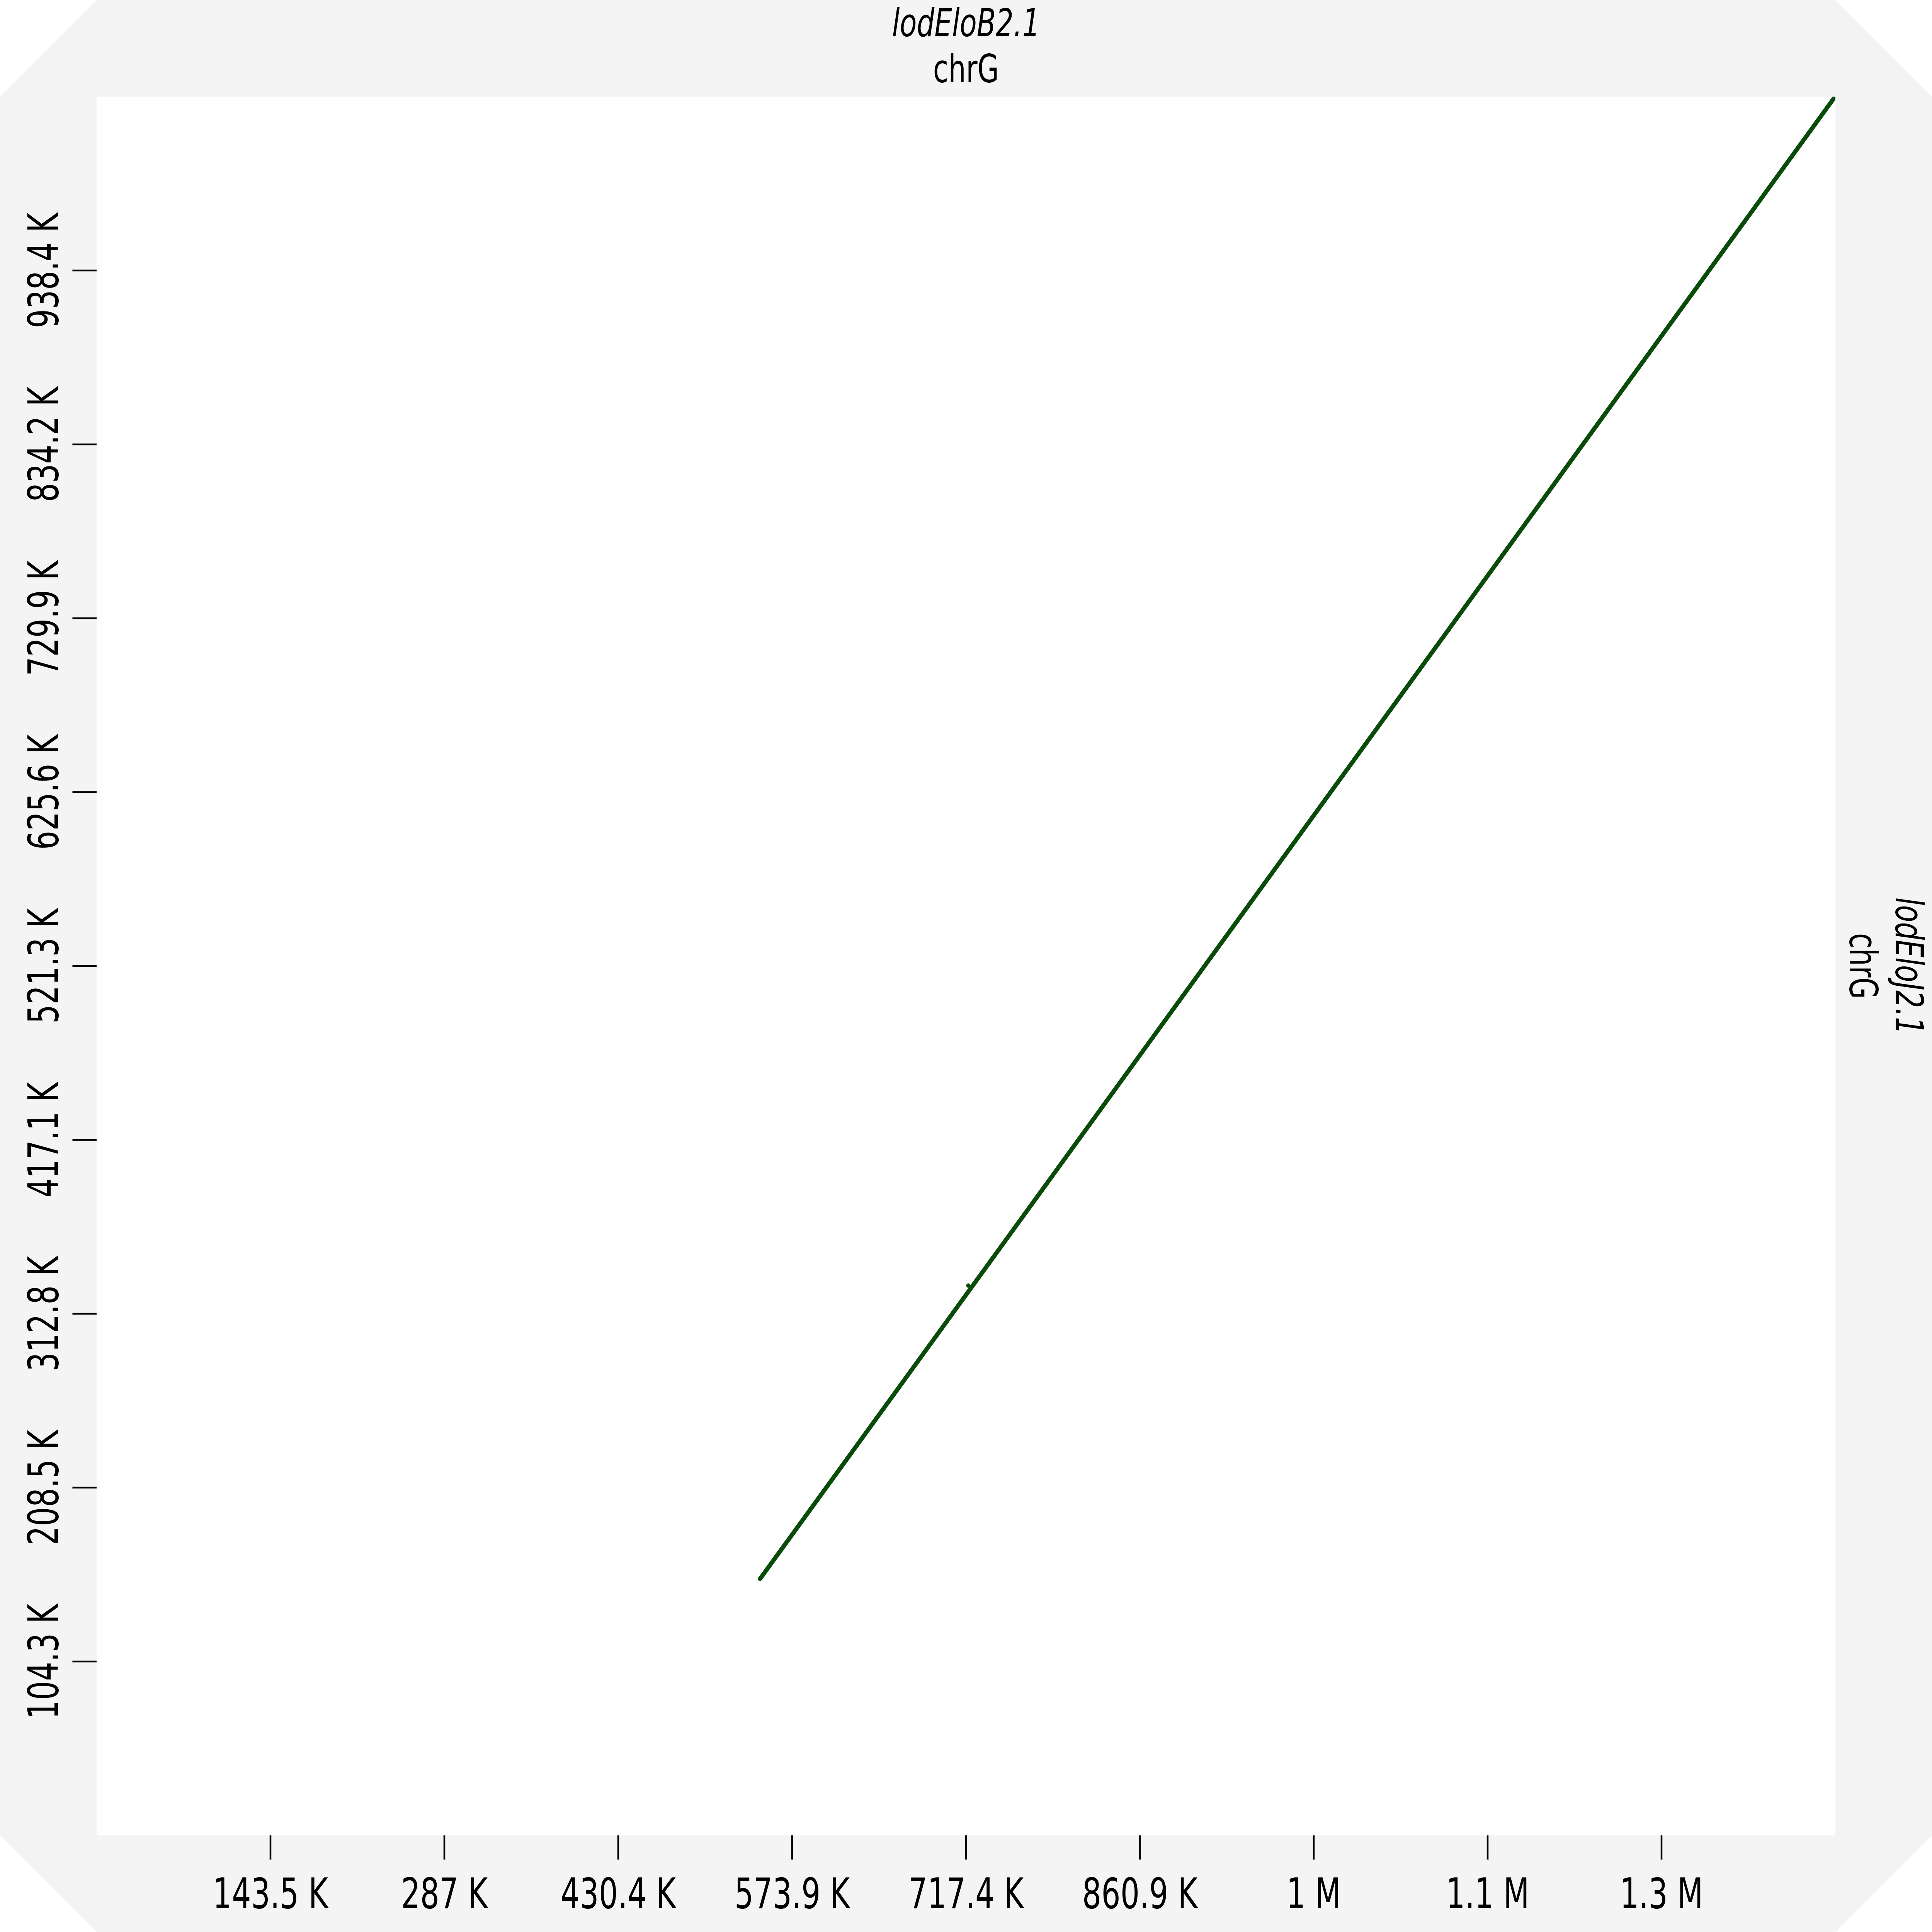
\includegraphics[width=.95\linewidth]{figures/lodelo/map_BG_JG.png}
%		\caption{Alignment between chromosome G of B2 and J2.}
%	\end{subfigure}%
%	\begin{subfigure}[b]{0.46\textwidth}
%		\centering
%		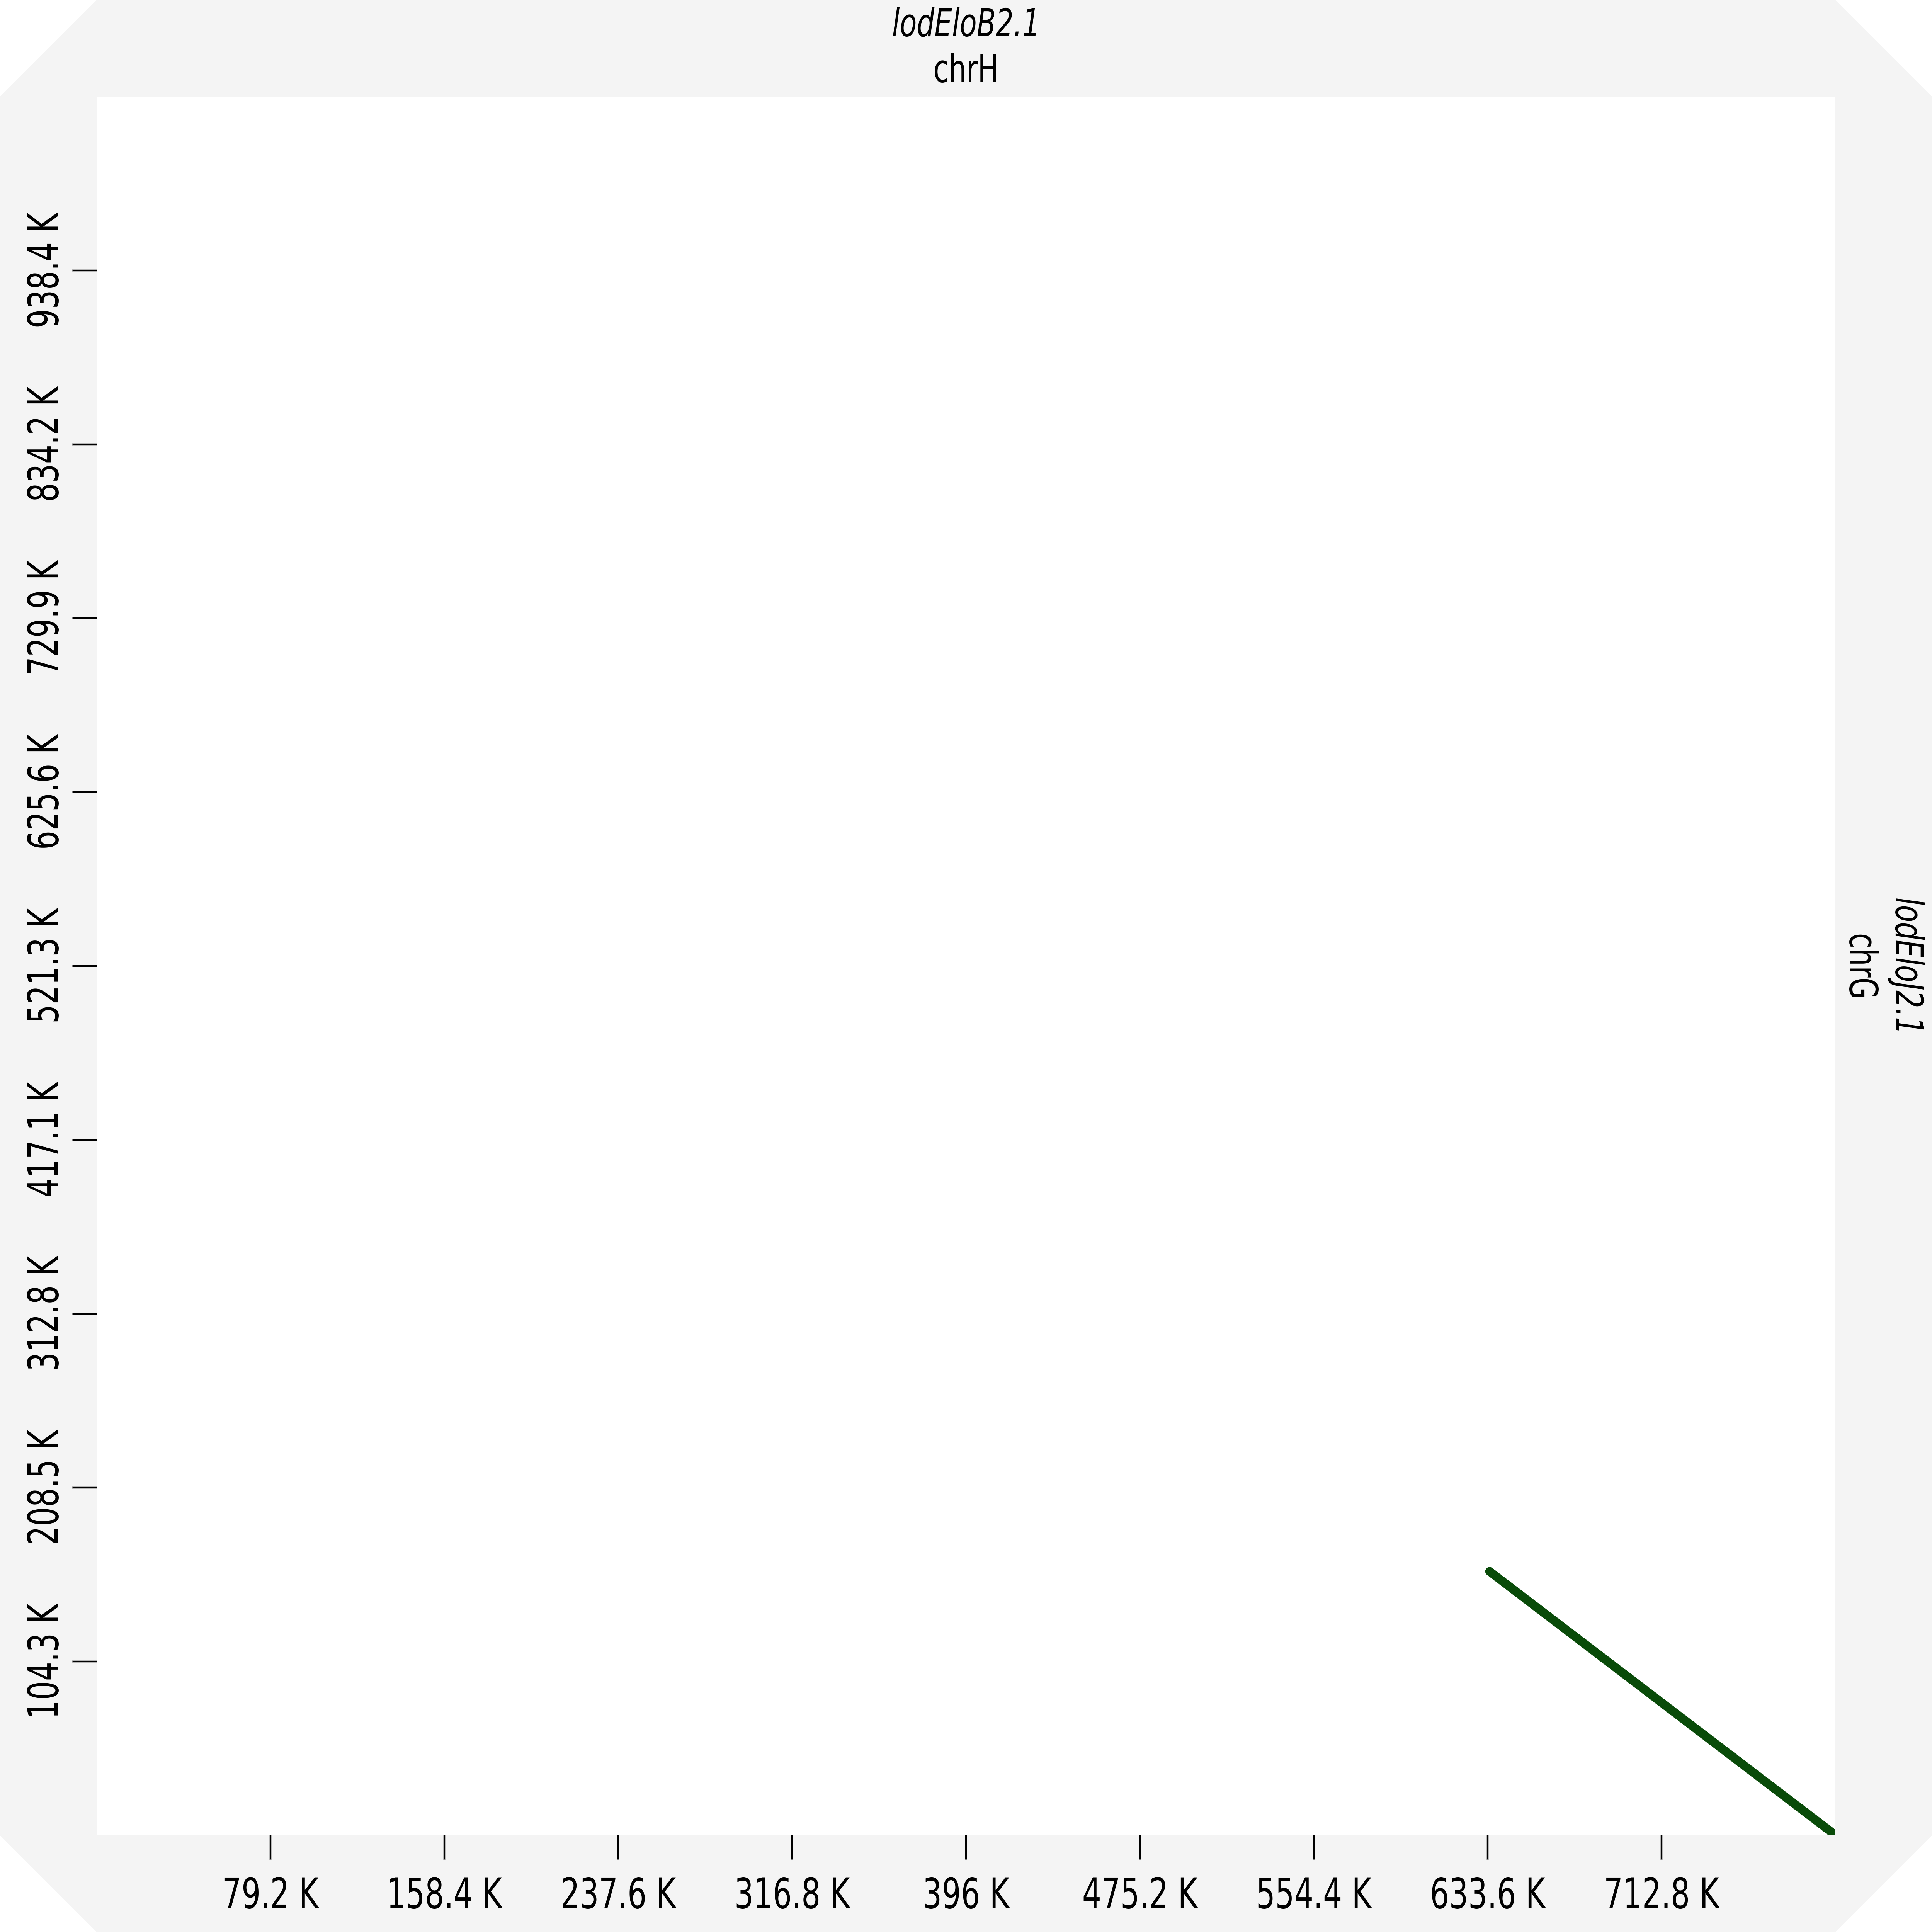
\includegraphics[width=.95\linewidth]{figures/lodelo/map_BH_JG.png}
%		\caption{Alignment between chromosome H of B2 and chromosome G J2.}
%	\end{subfigure}
%	\begin{subfigure}[b]{0.46\textwidth}
%		\centering
%		\caption{Alignment between chromosome C of B2 and J2.}
%	\end{subfigure}
%	\begin{subfigure}[b]{0.46\textwidth}
%		\centering
%		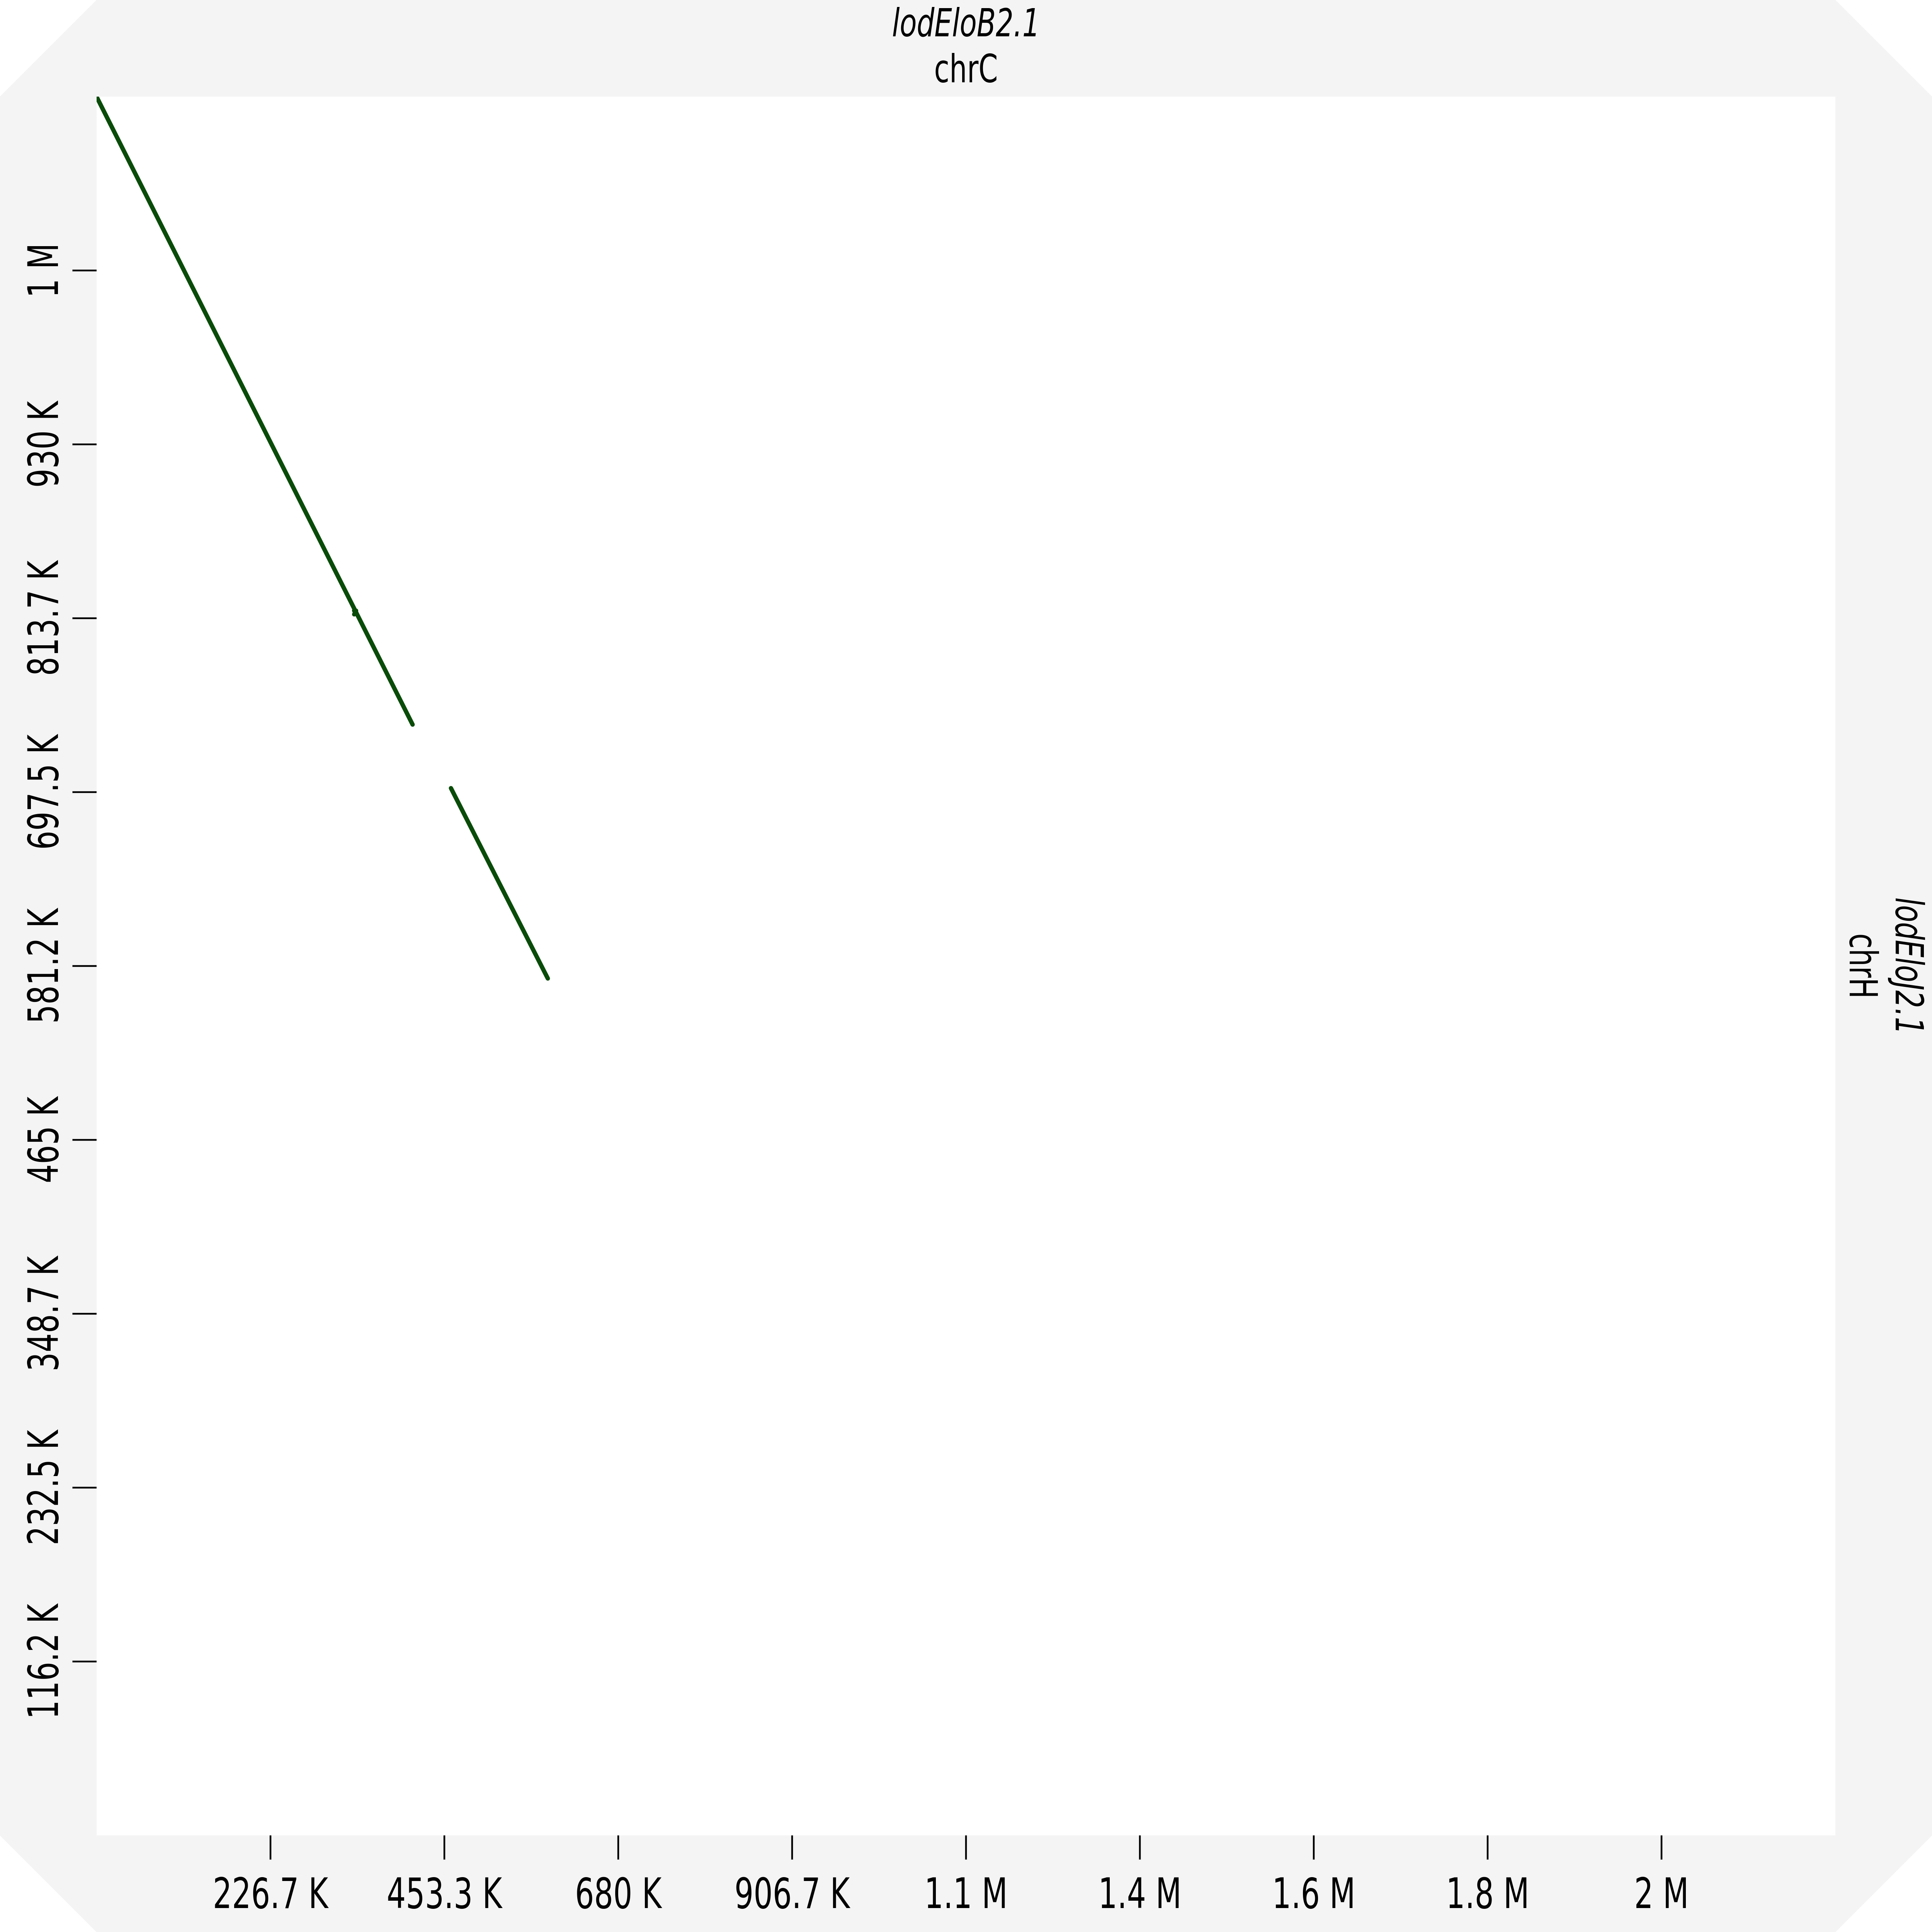
\includegraphics[width=.95\linewidth]{figures/lodelo/map_BC_JH.png}
%		\caption{Alignment between chromosome C of B2 and chromosome H of J2.}
%	\end{subfigure}
%	\caption{Dot-plot of the mapping of the resolved chromosomes of samples B2 and J2 for chromosomes C,G and H using D-Genies~\cite{dgenies} shows how large chunks of DNA is harbored into different chromosomes depending on the sample. Alignments were obtained using \wfmash \texttt{-p90 -s10000}.}
%	\label{fig:lodelo_dotplot-alignments}
%\end{figure}

%The consortium my phd fellowship belongs to, the EU Commission founded Marie Curie ITN Alpaca (Algorithms for Pangenomic computational analysis) consortium~\cite{alpacawebsite}, organized a winter wet-lab school to give a small training on how the processing of preparing samples for sequencing works, in order to improve the knowledge on the full stack of processes done to obtain genomes from biological samples of the medically interesting yeast strain of \lodelo. From 11 different samples, we generated long (ONT) reads, in collaboration with a lab at the Comenius University in Bratislava, Slovakia. We divided into several groups to perform different genomic analyses on it. One of these team, the one I was in, was tasked on building a pangenome reference of \lodelo. \\ 
%We sequenced,  The computational work I present here was done in collaboration with members of the consortium, in large part by Simon Heumos, whom I would like to thank for the time spent discussing and working together.

\subsection{\emph{Lodderomyces elongisporus}: genetic characteristichs, interest and used data}
\emph{Lodderomyces elongisporus} is a diploid yeast that has been isolated from, among many sources, humans and it is recently emerging as pathogenic. It is phylogenetically placed in the Candida clade and the size of its genome is usually between 15 and 16 Mb, 2 orders of magnitude smaller than a human genome~\cite{Lodderomyces}. Its DNA is organized into 8 chromosomes, that here will be referred in alphabetical order and decreasing size A to H, from around 3.5Mbp of chr A to 800 Kbp of chr H, plus a 35 Kbp mitochondrial DNA. Our analysis shows that it has a stable core genome of ~13Mbp, as shown in section~\ref{sec:core_pg}. 
Increasing reports of (mostly bloodstream) infection in mainly immunosuppressed adults makes it an increasingly important subject of studies\cite{lodelo_pathogen,lodelo_fatal,lodelo_meningitis,lodelo_bloodstream}: it also got recent attention when an outbreak was reported occurring in a neonatal ICU in Dheli, India from September 2021 to February 2022 with 1 death\cite{lodelo_india}.\\
Samples sequenced by us were called in alphabetical order, followed with a number greater or equal than 0 that denoted the quality of the assembly. Moreover, one sample, B2, for which a member of the consortium produced a high quality assembly after manual curation, was used as relative reference in the cohort. Another sample, J2, was also fully resolved into chromosomes while the others were assembled into contigs.

\begin{table}
	\centering
	\begin{tabular}{| c | c | c | c | c | c | c | c | c | c | c | c | c | c |}
		\hline
		filename     &   total length   & number of sequences & mean length &    longest & shortest     &   N count & Gaps &   N50  &   N50n  &  N70 &    N70n &   N90 &    N90n \\
		\hline
		A1 & 15699113 & 25 & 627964.52 & 2595744 & 3907 & 0 & 0 & 1354781 & 5 & 938474 & 8 & 414196 & 13 \\
		B2 & 15485469 & 7 &  2212209.86 & 4493495 & 35166 & 0 & 0 & 3516991 & 2 & 2001278 & 4 & 1643619 & 5 \\
		C0 & 15532065 & 20 & 776603.25 & 3532941 & 810 & 0 & 0 & 1331232 & 4 & 1222310 & 6 & 835847 & 9 \\
		D0 & 15507665 & 17 & 912215.59 & 3532853 & 5008 & 0 & 0 & 2160581 & 3 & 1885061 & 5 & 740828 & 7 \\
		E0 & 15332588 & 18 & 851810.44 & 3544471 & 3228 & 0 & 0 & 1992182 & 3 & 1040518 & 6 & 418294 & 10 \\
		F1 & 15664073 & 21 & 745908.24 & 3548518 & 1282 & 0 & 0 & 2165076 & 3 & 1245669 & 5 & 440649 & 9 \\
		G0 & 15636520 & 19 & 822974.74 & 3548910 & 550 & 0 & 0 & 1697956 & 4 & 1657398 & 5 & 527890 & 9 \\
		H0 & 15601346 & 21 & 742921.24 & 3549008 & 6842 & 0 & 0 & 2170489 & 3 & 1247137 & 5 & 469363 & 10 \\
		I1 & 15639882 & 30 & 521329.40 & 3622524 & 536 & 0 & 0 & 1999295 & 3 & 1636379 & 5 & 384387 & 10 \\
		J2 & 15425942 & 9 & 1713993.56 & 3543738 & 35442 & 0 & 0 & 2157297 & 3 & 1647795 & 5 & 1162477 & 7 \\
		K0 & 15752744 & 16 & 984546.50 & 3534745 & 19835 & 0 & 0 & 1631500 & 4 & 1305577 & 6 & 684340 & 9 \\
		\hline
	\end{tabular}
\end{table}

\subsection{Building ad hoc pangenome reference}
We produced a \dbg of the assemblies using \bifrost, but their usefulness remains limited for visual analysis of complex biological events interpretation and study.\\
Figure~\ref{fig:lodelo_dbg} shows the visualization of the \dbg for \kmer length equal to 25: redundant parts of the genome make the graph collapse. This is the same phenomenon previously described for human genomes, as better insight can be acquired when just a small region is visualized. 
De Bruijn Graphs can instead be useful for to produce quite straightforward whole-genome alignment- and reference-free phylogenetic analysis in a fraction of time required by competitor methods that use all vs. all alignment. The tool \sans~\cite{sans} can process directly a \bifrost generated \ccdbg to estimate the phylogenetic splits between the genomes contained in the graph. Figure~\ref{fig:dbg_phyl} shows the visualization of the phylogenetic network produced by \sans using the tool \splitstree~\cite{splitstree}. This results shows how \dbgs are quite powerful when applied to specific applications.\\
\begin{figure}[h!]
	\centering
	\begin{subfigure}[b]{0.75\textwidth}
		\centering
		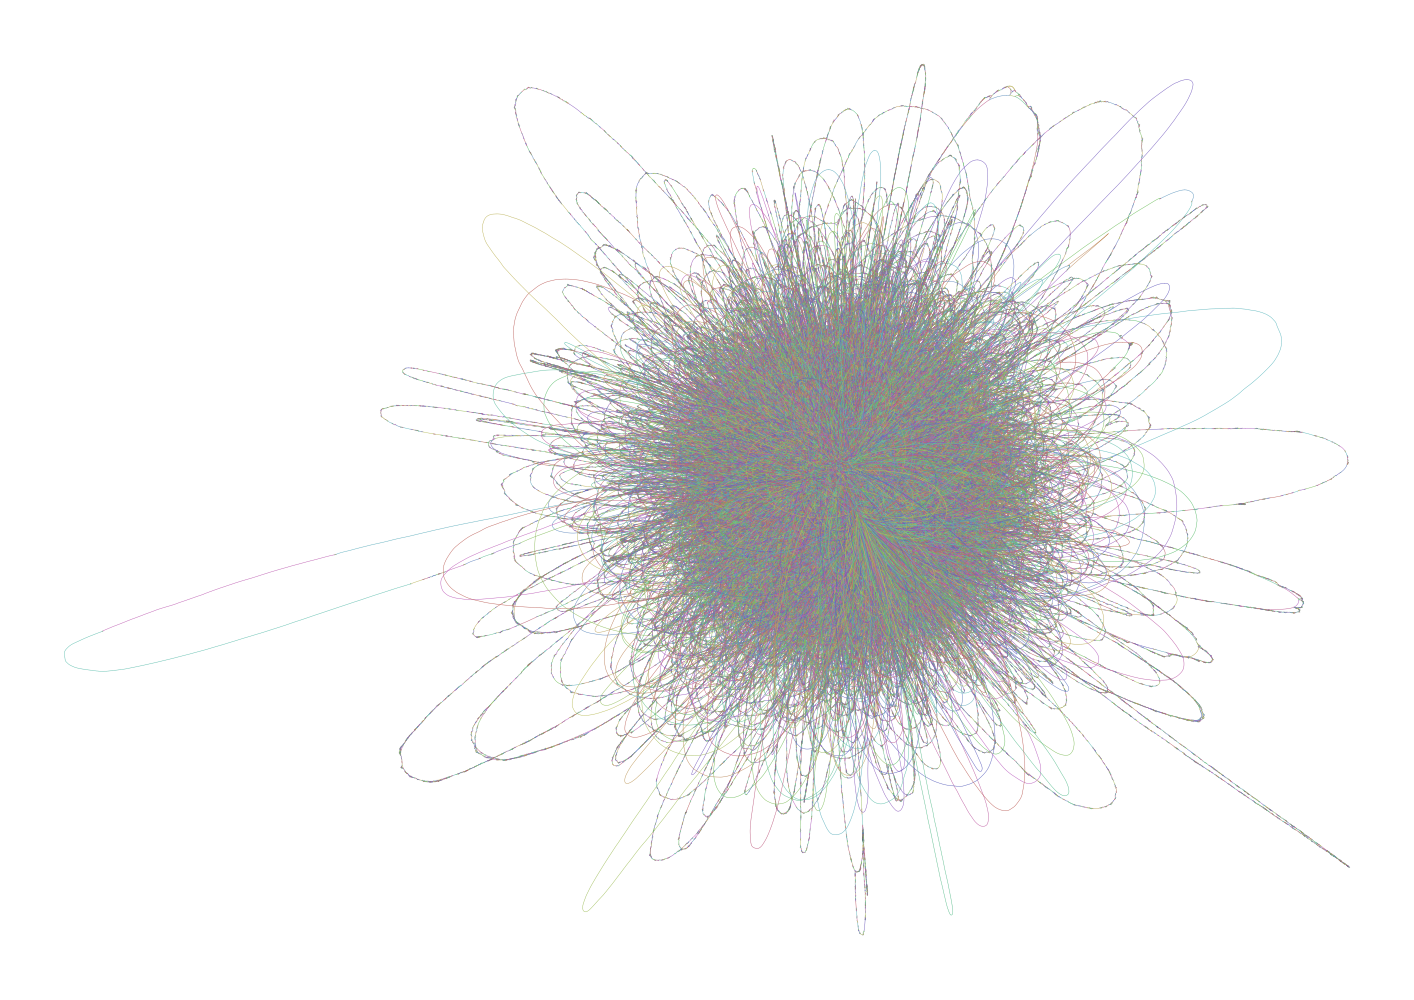
\includegraphics[width=1\linewidth]{figures/lodelo/lodElo_k25.png}
		\caption{\bandage visualization of the pangenome \dbg of the cohort of 11 \lodelo strains. As for human genomes, visualization of the whole data offers no particular insight, apart from the large variations visible on the rounded parts away from the dense part.}
		\label{fig:lodelo_dbg}
	\end{subfigure}%
	\\
	\begin{subfigure}[b]{0.75\textwidth}
		\centering
		\includegraphics[width=1\linewidth]{figures/lodelo/direct_nobei.png}
		\caption{\splitstree visualization of the phylogeny network generated using \sans from the \ccdbg constructed using \bifrost.}
		\label{fig:dbg_phyl}
	\end{subfigure}%
	\caption[\ccdbg representation and phylogeny analysis of the \lodelo pangenome.]{Visualization of the \ccdbg representation and phylogeny analysis of the \lodelo pangenome.}
\end{figure}
Given high quality assemblies generated by the sequences of these 11 samples, we decided to also build a pangenome graph with small variant resolution using \pggb and \mcactus, in a similar way to what has been done with the Human Draft Pangenome Reference~\cite{hdpr}. It is important to notice that in order to produce the best biological correct result, several rounds of parameter tuning and manual curation are needed, with knowledge far superior of the one of a first-time user.\\
The first step to build such pangenomes is to divide the genome assemblies into communities of sequences belonging to chromosomes.

%As explained before, variation graphs generation is given by communities separation. \pggb works by building a single graph from a given community, so it fits well for this specific use-case: by grouping together the contigs corresponding to the three chromosomes where the recombination occurred, the pipeline should produce a graph that consider this event.
\subsubsection{Determining chromosomal communities}
Variation graphs construction pipelines use mapping or alignment between the input set of genomes to infer graphs. Their first step consists in grouping the sequences from the assemblies into communities representing a chromosome in order to run a single computation instance and produce a separate graph for each of them. The final graph is then given by joining together the output of each group. This means that without any pre-processing, no inter-chromosomal event can be detected.\\ 
In this specific use-case, in order to identify inter-chromosomal events, contigs associated to any of the 3 chromosomes conjectured to be part of the rearrangement had to fall into the same community and be provided together in input to the pipeline. This would ensure that, if such rearrangement exists, it would produce a feature in the graph that would show as a tangle between the chromosomes.\\
As the rest of the assemblies, with the exception of the J2 sample, were not resolved into single chromosomes, each of them was aligned to the reference B2 using \wfmash alignment segment size of 10k and 95\% sequence identity (and lower segment size, 90\% sequence identity if unmapped). The identity scores of the alignment of the genomes to the reference B2 assembly is shown in figure~\ref{fig:lodelo_alignment_scores}. From this alignment, contigs were assigned to the chromosomal community to which they best mapped. Finally, the ones of chromosome C, G and H were grouped into a single one.
\begin{figure}[h!]
	\centering
	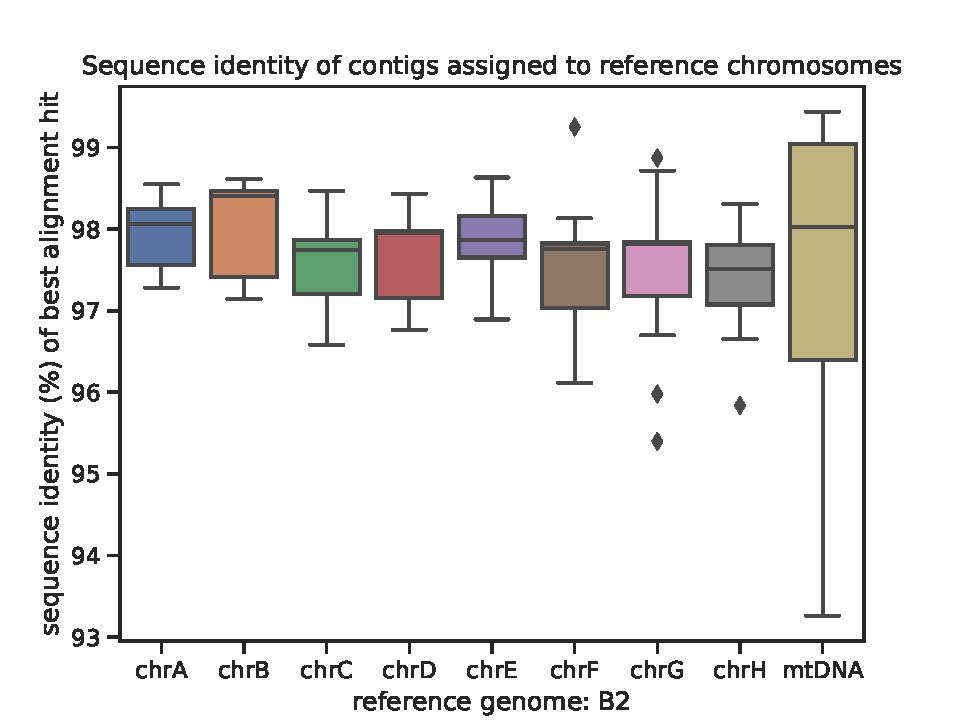
\includegraphics[width=.8\linewidth]{figures/lodelo/Alignment_scores.pdf}
	\caption[Sequence Identity of \lodelo samples's contigs assigned to reference chromosomes.]{Sequence Identity of contigs assigned to reference chromosomes. Image produced using a pipeline developed by Simon Heumos.}
	\label{fig:lodelo_alignment_scores}
\end{figure}

\subsubsection{Producing a variation graph using pggb}
As \pggb uses all-vs-all alignment of a collection of sequence as first step to infer the graph, it enables the representation of recombination among chromosomes placed inside the same community, as seen also for human acrocentric chromosomes~\cite{Guarracino2023}.\\
By simply running the \texttt{nextflow/pangenome} (\pggb) pipeline, we were able to produce a first pangenome representation of the 11 yeast strains. The tangle visible in figure~\ref{fig:lodelo_gfaestus} clearly shows the recombination happening between the three chromosomes. This work was mainly done by Simon Heumos and the graph shown in figure ~\ref{fig:lodelo_gfaestus} is the result of more than 25 rounds of parameters tuning.
The detection of the event with a variation graph using \pggb encouraged the effort to produce a similar representation with \mcactus, a pipeline that is not designed to construct grouped chromosomes pangenomes.
\begin{figure}[h!]
	\centering
	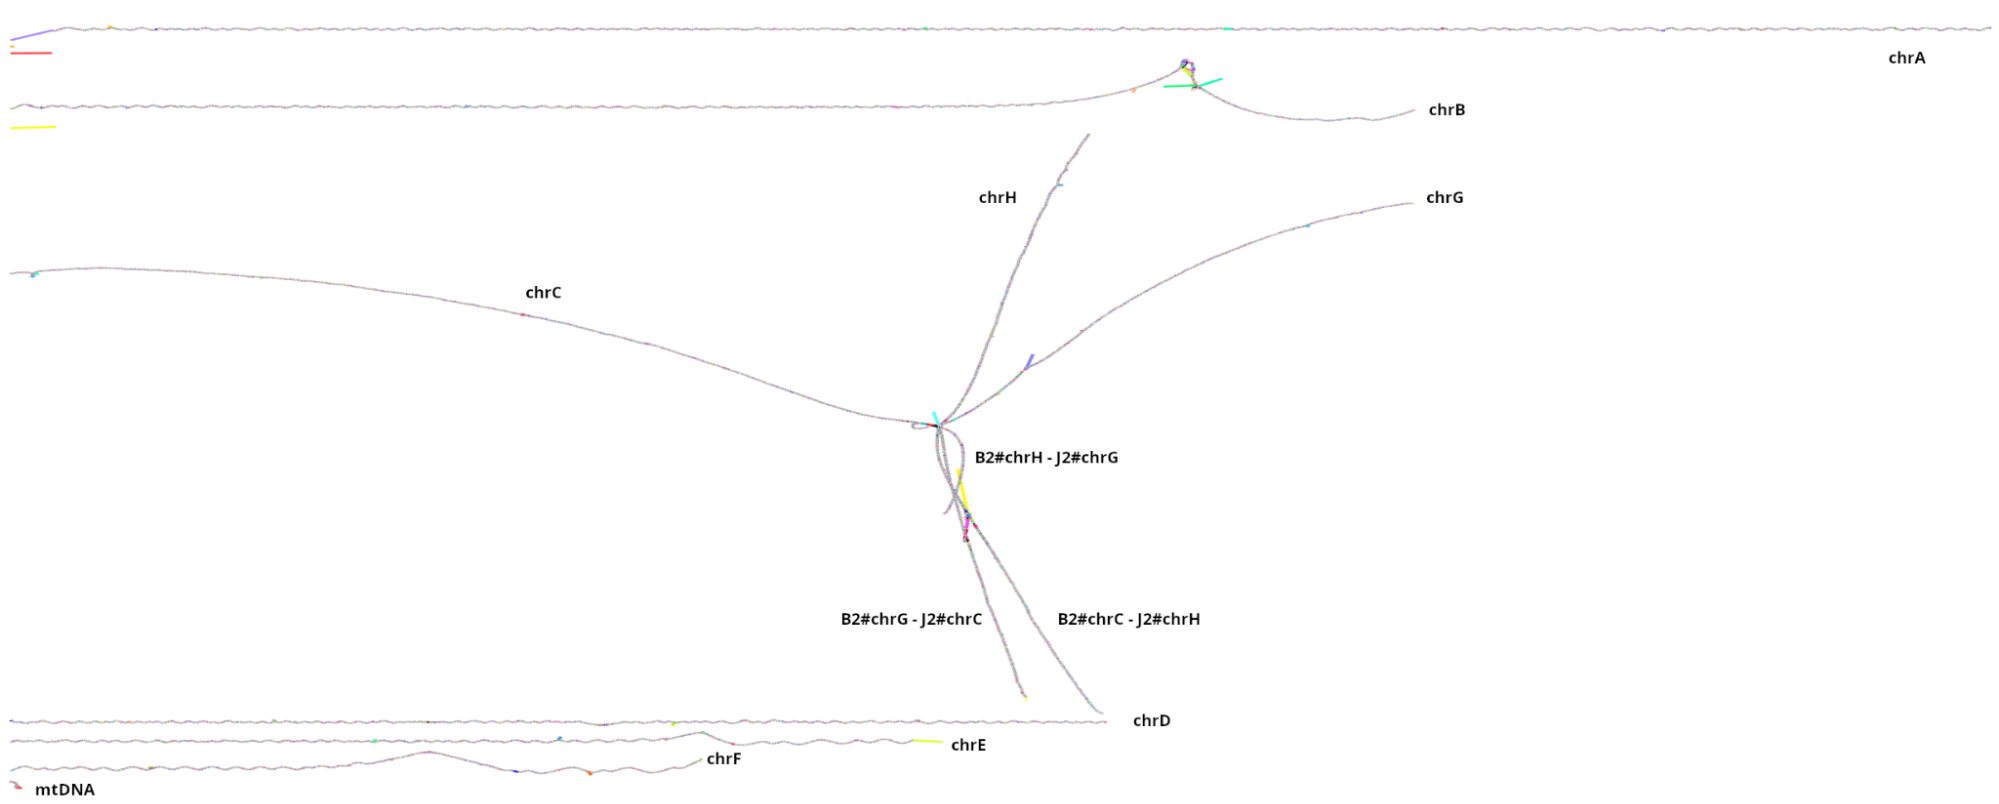
\includegraphics[width=.8\linewidth]{figures/lodelo/pggb_full.png}
	\caption[\gfaestus visualization of a \lodelo variation graph.]{\gfaestus visualization of the \pggb variation graph of the 11 \lodelo samples. Image produced by Simon Heumos.}
	\label{fig:lodelo_gfaestus}
\end{figure}


\subsubsection{Overcoming \mcactus limitation by modifying both the data and the pipeline}
In order to produce a graph that represents variation between multiple chromosome with \mcactus, a custom pipeline has to be used. \mcactus communities are implicitly inferred by the first step, performed by \minigraph. For this tool, the chromosomes present in the first reference genome given as input are used as communities and backbone for the whole graph and no sequence can be both assigned to different chromosome. This is an intrinsic characteristic of \minigraph and cannot be changed with input parameters: it means that there is no feature to have chromosome C,G and H considered together in input.\\
To try to overcome this limitation of the approach we tried to produce a graph that respected the condition of having the three chromosome inside the same connected component, at the cost of producing a representation that was not biologically correct. We therefore produced a chimeric contig consisting of the concatenation of the three chromosomes assemblies of the B2 sample. The rationale was to provide the 3 chromosomes chained together as a single backbone in the \minigraph construction step. This would allow sequences to be mapped to any of chr C, G and H to be considered together in the subsequent steps of alignment and graph the \mcactus pipeline. The expectation was to therefore produce a graph that showed the recombination from the mapping of the contigs of the other genomes. \\
By building a graph using \minigraph with the chimeric chromosome CGH and all the contigs of the other genomes assigned to chromsome C, G and H does not represent any recombination event, as can be seen in figure~\ref{fig:cgh_mingraph}. This was somewhat expected, as it is known that \minigraph does not also consider inversion between genomes.
When the complete modified pipeline of \mcactus is run, it is possible to see the tangle between the chromosomes, as shown in figures~\ref{fig:cgh_mcactus}~\ref{fig:lodelo_graph_tangle}.
\begin{figure}[h!]
	\centering
	\begin{subfigure}[b]{\textwidth}
		\centering
		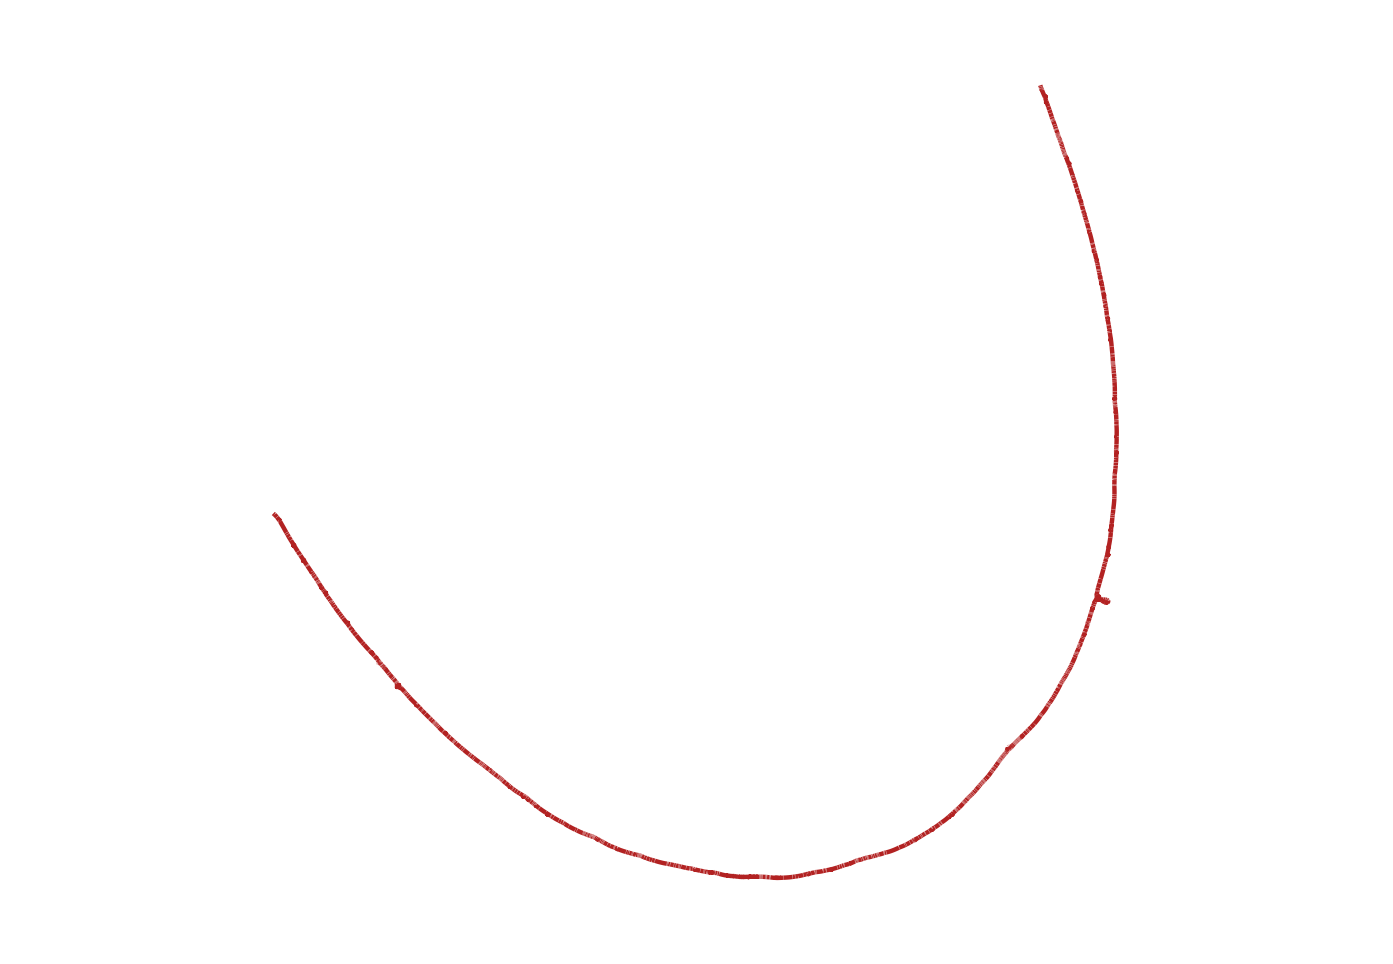
\includegraphics[width=.4\linewidth]{figures/lodelo/minigraph_cgh.png}
		\caption{Graph of chimeric chromosome CGH from sample B2 and all the contigs of the other genomes aligning to it produced with \minigraph. The graph is linear and no inter-chromosomal event is visible.}
		\label{fig:cgh_mingraph}
	\end{subfigure}%

	\begin{subfigure}[b]{\textwidth}
		\centering
		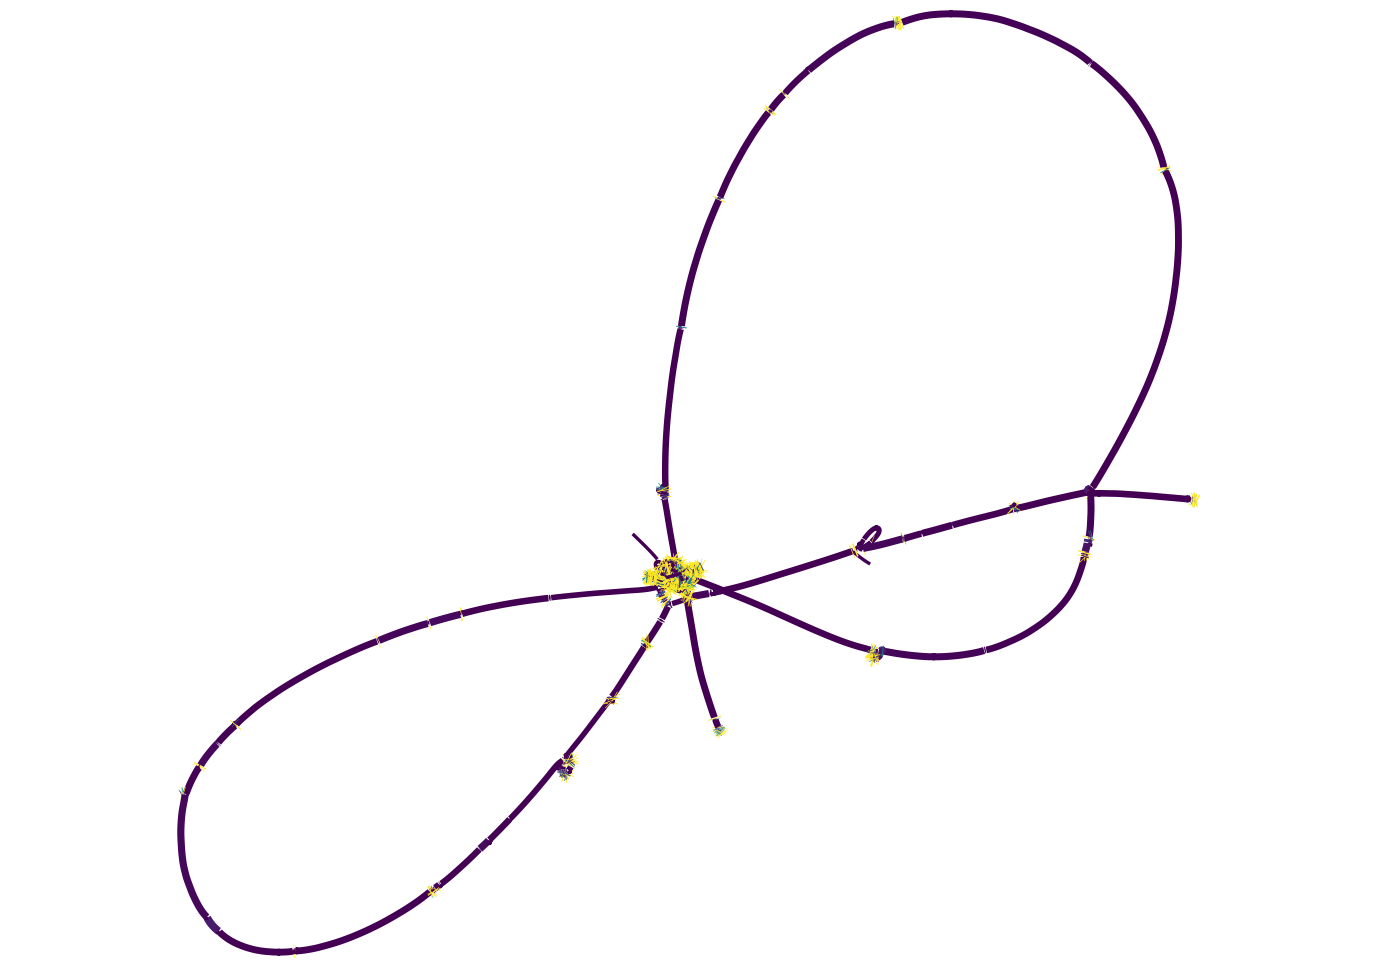
\includegraphics[width=.4\linewidth]{figures/lodelo/mcactus_cgh_u1000_by_depth.png}
		\caption{The graph after all the other steps of the \mcactus pipeline, colored by depth, after simplification of variants < 1kbp using the command \gfatools  \texttt{asm -b 1000 -u}. The large recombination event is now visible.}
		\label{fig:cgh_mcactus}
	\end{subfigure}
	\caption[Difference in output between \minigraph and \mcactus.]{Difference in output between \minigraph and \mcactus of the chimeric graph produced to visualize the inter-chromosomal event between C,G and H.}
	\label{fig:chromosome_cgh_minigraph}
\end{figure}

\subsection{Representing translocation events from groups of genomes}
Applying simple community separation on the all vs all alignment of the contigs, like the one suggested in the manual of \pggb, does not help confirming the hypothesis, mainly because of segment length selection. Figure~\ref{fig:lodelo_communities} shows community detection using Louvain algorithm on the contig network inferred by all vs all alignment.
\begin{figure}[h!]
	\centering
	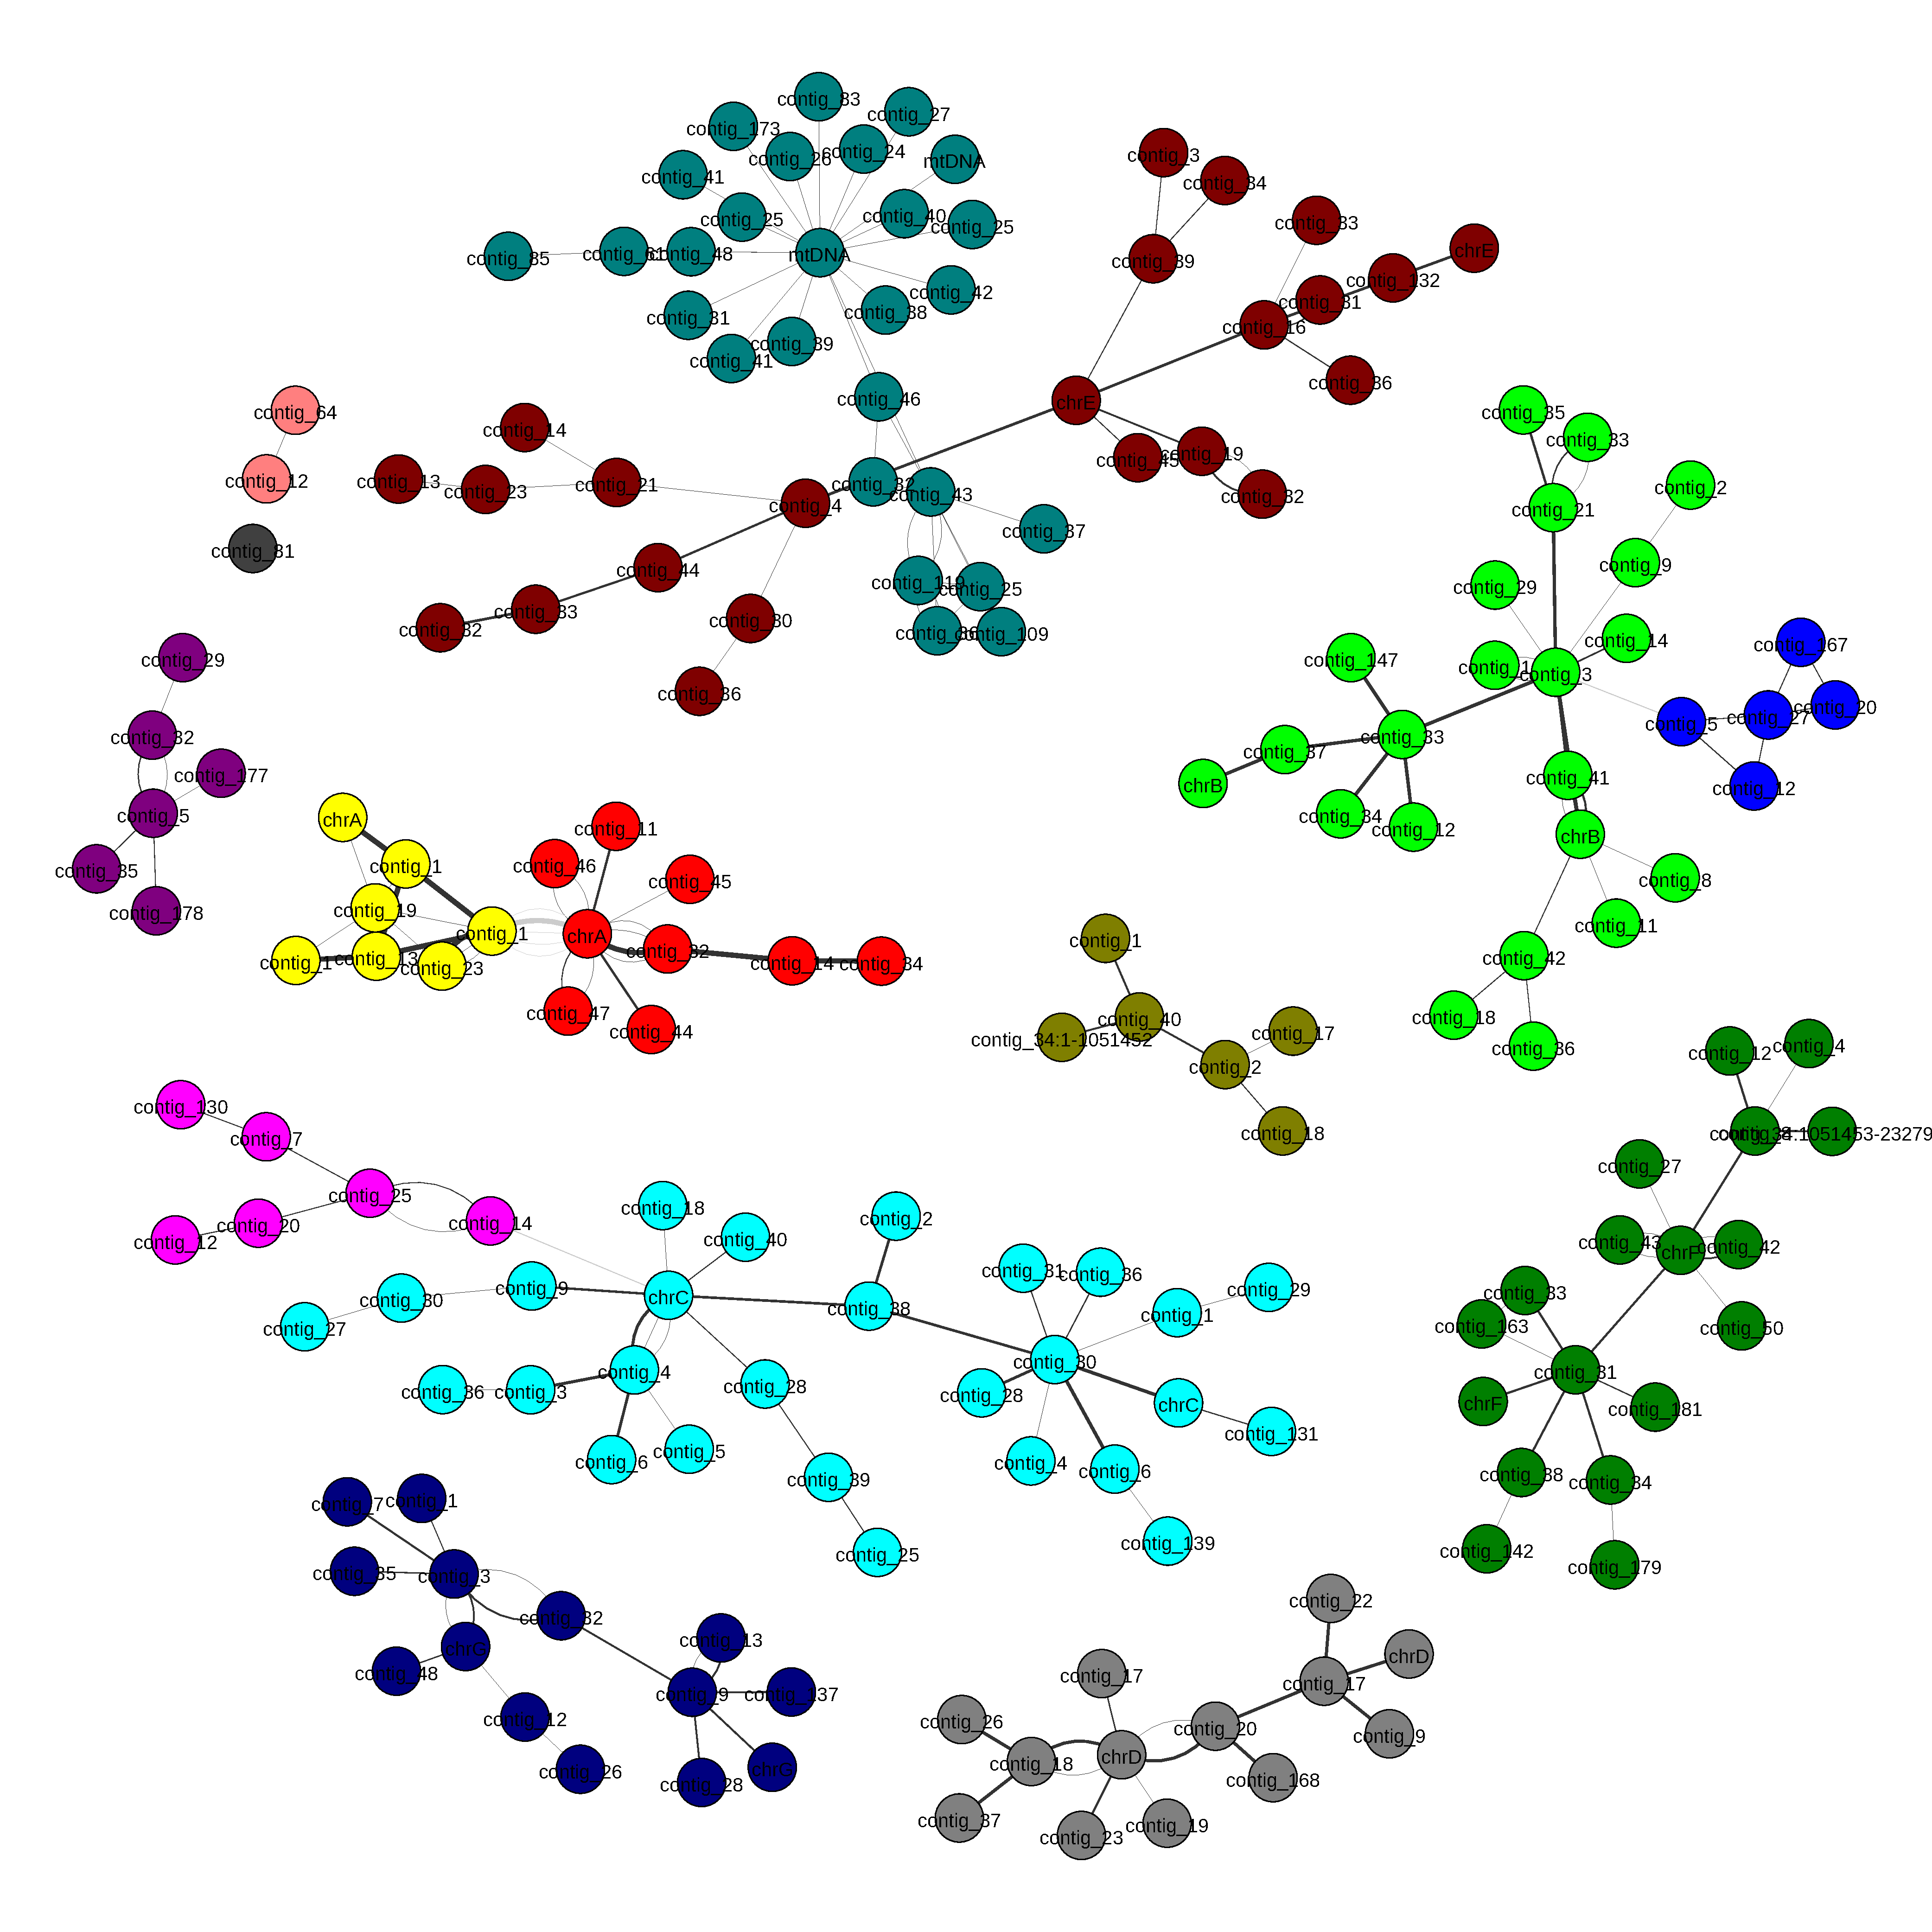
\includegraphics[width=.4\linewidth]{figures/lodelo/alingment_communities.pdf}
	\caption[Community partition of the contigs to detect inter-chromosome events.]{Community partition of the contigs based on all-vs-all alignment scores.}
	\label{fig:lodelo_communities}
\end{figure}
This inter-chromosomal rearrangement is instead detectable using linear whole-genome assembly based tools. By aligning J2 to the relative reference genomes B2 with \wfmash and then looking for syntenies and rearrangements with \syri, it is possible to detect syntenic path (longest set of co-linear regions), structural rearrangements (inversions, translocations, and duplications)~\cite{syri}. Figure~\ref{fig:plotsr_synteny} shows the detected rearrangements and duplications between the 3 chromosomes using \plotsr~\cite{plotsr}.
While figure~\ref{fig:plotsr_synteny} shows in a clear way the kind of inter-chromosomal variation between the 2 strains, \syri does work only with genomes resolved to chromosome level. This means that such analysis is not possible on the whole cohort using standard linear reference tools. 
\begin{figure}[h!]
	\centering
	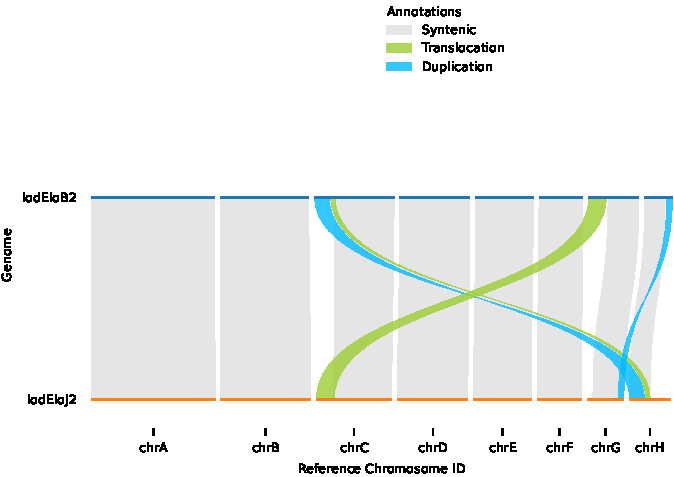
\includegraphics[width=.8\linewidth]{figures/lodelo/plotsr.pdf}
	\caption[Linear reference visualization of the \lodelo inter-chromosomal recombination.]{\plotsr visualization of the inter-chromosomal recombination detected using \wfmash and \syri.}
	\label{fig:plotsr_synteny}
\end{figure}
It is therefore possible to visualize the tangle that emerges from the graph generated with \mcactus. 
\begin{figure}[h!]
	\centering
	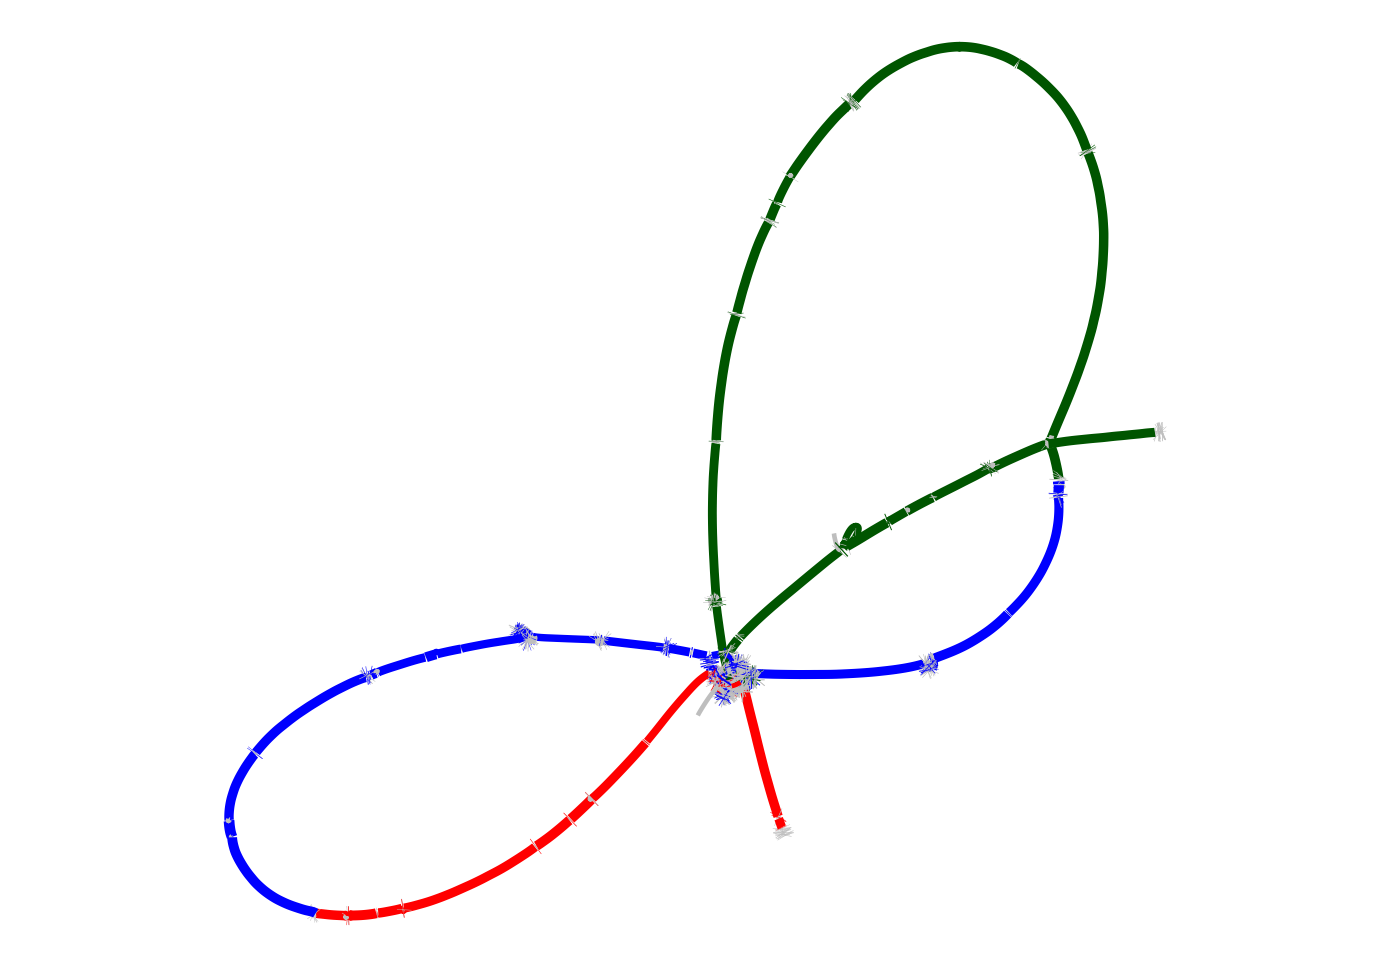
\includegraphics[width=.8\linewidth]{figures/lodelo/tangle_chrCGH_B2_Cgreen_Gblue_Hred.png}
	\caption[Visualization of chromosomes tangle in the \mcactus variation graph.]{ \bandage visualization of the tangle of chromosomes C, G and H in the \mcactus variation graph. Nodes are colored based on \minigraph alignment of chromosome C (dark green), G (blue) and H (red) of the reference assembly B2. The three chromosomes are bound together because of the construction.}
	\label{fig:lodelo_graph_tangle}
\end{figure}

\subsection{Estimating core genome and pangenome growth}
\label{sec:core_pg}
Finally, pangenome graphs are also useful to quantify the part of the genome that is shared between genomes (what is called core-genome) and the parts that are mostly shared or private to each one. It is also interesting to estimate its growth, i.e. to measure how much the total genomic content grows with the increase of the size of the sample. These metrics can be obtained by using the tool \panacus~\cite{panacus}. \texttt{Panacus} is a tool that calculates coverage distributions of countable elements in variation graphs: it uses paths to detect how many genomes are associated to any node, edge or basepair of the pangenome graph. From these distribution it computes the pangenome growth and core curves as function of the number of genomes.\\
Calculating these metrics can be used to validate that the two variation graphs built with \pggb and \mcactus agree on the underlying genetic distribution of the input sample.\\
Figure~\ref{fig:panacus} shows very concordant metrics for the two variation graphs. First, they show similar basepair coverage histogram, that highlight a great portion of genome shared by all the samples, and a non-negligible share of sequences that are private to each genome (~1.5Mbp in total). Secondly, both growth curves show similar pattern, that seems plateauing. This is also highlighted by the fraction of new base pairs introduced by each sample, that decreases from ~700k new basepairs with the new sample to less than ~142k base pairs in on the 11th genome. Finally, the core pangenome can be estimated by the basepairs that are spelled by all the genomes in the graph: the computed value for the 11 samples is ~13,2 Mbp for \pggb and ~13,6 Mbp for \mcactus. The variability in the results are expected and due to different graph construction methods.
\begin{figure}[h!]
	\centering
	\begin{subfigure}[b]{0.45\textwidth}
		\centering
		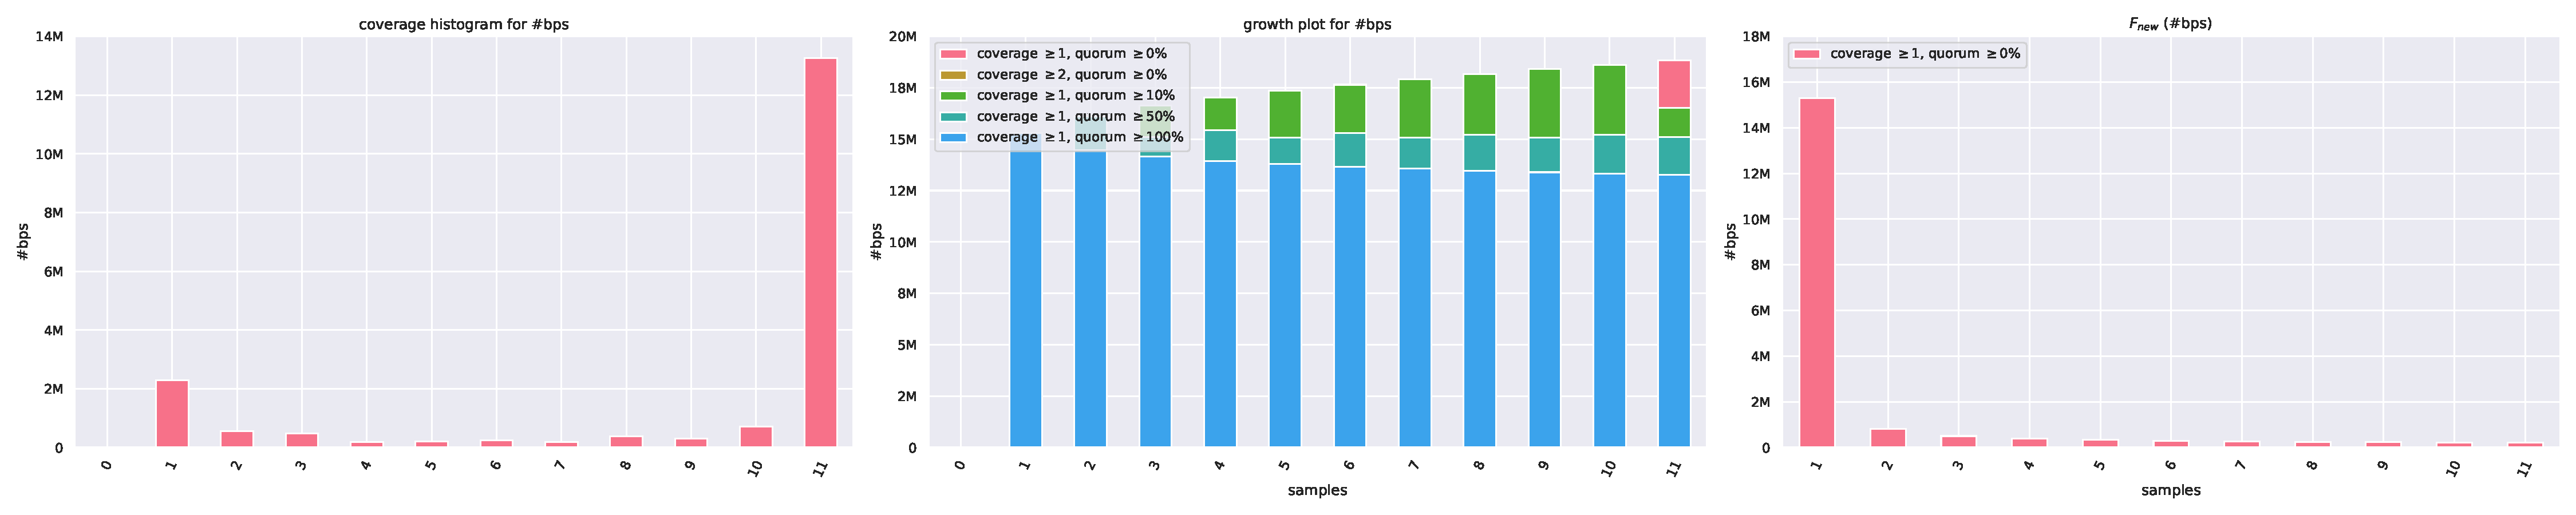
\includegraphics[angle=90,width=.7\textwidth]{figures/lodelo/lodelo_simon.histgrowth.pdf}
		\caption[\pggb pangenome.]{\pggb pangenome.}
	\end{subfigure}%
	\begin{subfigure}[b]{0.45\textwidth}
		\centering
		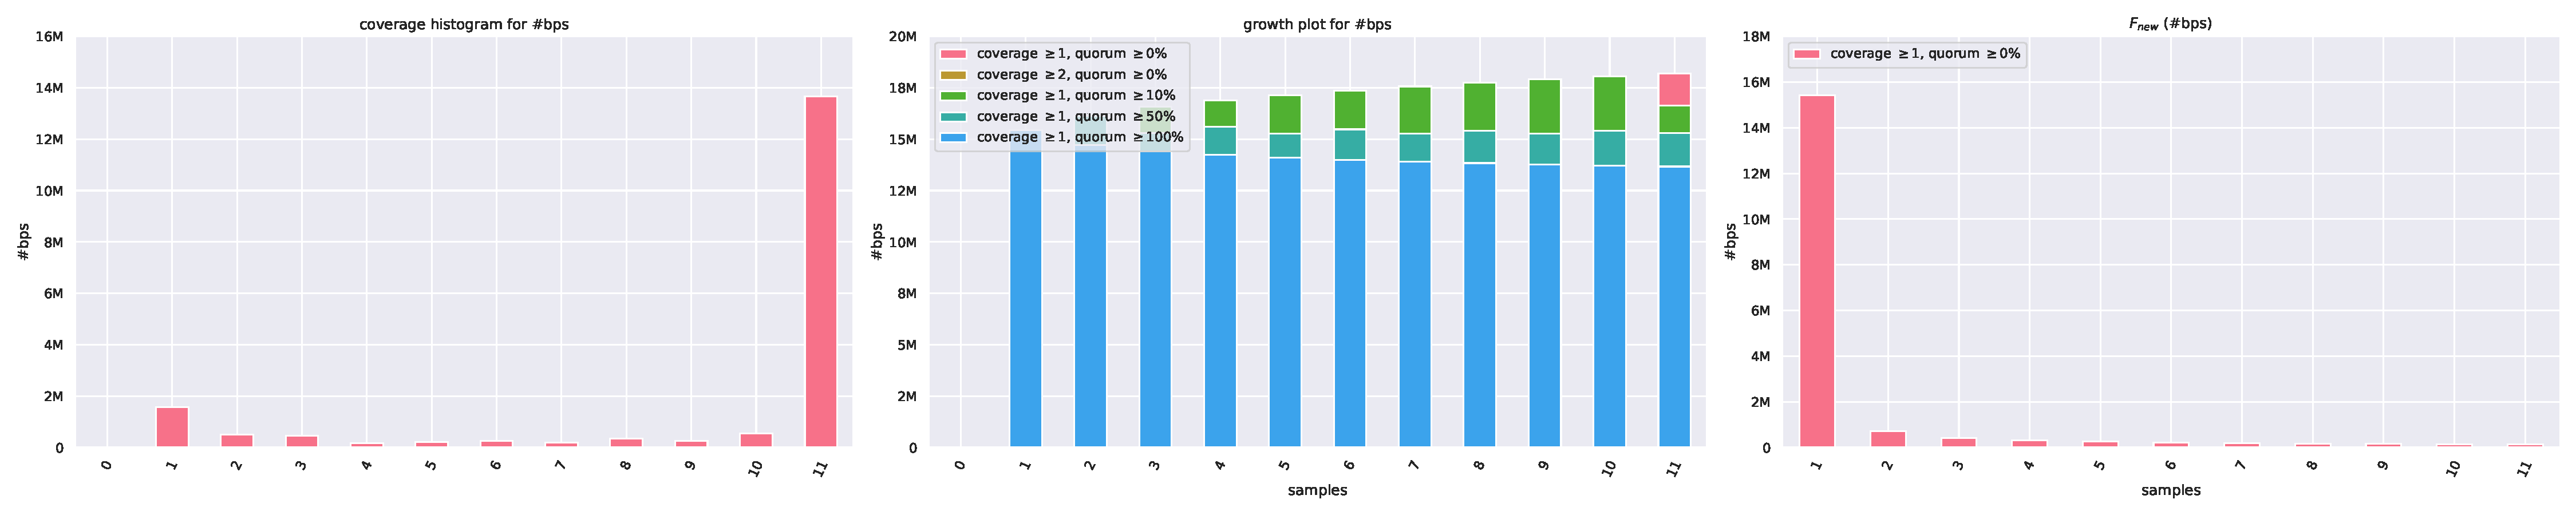
\includegraphics[angle=90,width=.7\textwidth]{figures/lodelo/lodelo_cactus.histgrowth.pdf}
		\caption[\mcactus pangenome.]{\mcactus pangenome.} 
	\end{subfigure}%
	\caption{Pangenome core and growth of \lodelo using variation graphs. \pggb graph generated by Simon Heumos.}
	\label{fig:panacus}
\end{figure}

\section{Conclusion and Perspectives}
The work presented above shows how pangenomes can serve as analysis platform of samples from same-strain yeast. \\
\dbg-based tools currently offer a limited range of possibilities, especially for lower sample sizes. They best serve as fast and memory-efficient container for large amounts of data that require simple interrogations like absence-presence queries. This model can nevertheless help answer simple biological questions on such small samples, like phylogenetic analysis shown in figure~\ref{fig:dbg_phyl}.\\
Variation Graphs on the other side are powerful and very useful on few genomes analysis as they can be built quickly enough and provide a well-established platform for downstream analysis tools. On the other side, there is still need to very labor-intensive manual revision of the output graphs to find the input parameters that produce the best result, as it took more than 25 rounds to find the best \pggb parameters to produce the graph shown in figure~\ref{fig:lodelo_gfaestus}. As they are produced on heuristics and not on mathematically defined concepts, each variation graphs-construction tool produces different results: in figure~\ref{fig:chrE_difference}, it is possible to see the difference 1d-representation of the small chromosome E between \pggb and \mcactus. Finally, in order to detect the inter-chromosomal rearrangement with \mcactus as in figure~\ref{fig:lodelo_graph_tangle}, I had to rewrite the pipeline and modify the input data. \\
Apart from the aforementioned limitations, that show how such methods are still more prototypes than sound and established tools, this analysis shows how much potential there is to improve the current state-of-the art in genomes analysis. Linear-sequences tools are based on well-established genome-to-genome comparison methods that fail to adapt to heterogeneous data, like different levels of assembly quality. As \syri fails to detect rearrangements on genomes that are not assembled to the chromosome level, variation graphs are able to show the variation among all samples, even if the majority of the genomes contain contigs. \\
This work is another display of the great potential pangenome approaches have. In the future it would be very interesting to build pipelines or develop tools that enable visualizations and straightforward analysis from variation graphs or \ccdbgs] to the same level as the current linear-genomes tools. As I have already conceptualized some possible approaches for \ccdbgs, in the future it would be useful to develop simple prototypes and test how fast and precise these would be.\\
In the future it would be very informative to produce a more comprehensive report of the work done by my group and me, together with the other groups that worked on analyzing these novel \lodelo samples, to offer a comprehensive view of how specific pangenomes can be built and used to provide improved genomic analysis capabilities.

\begin{figure}[t]
	\centering
	\begin{subfigure}[b]{0.8\textwidth}
		\centering
		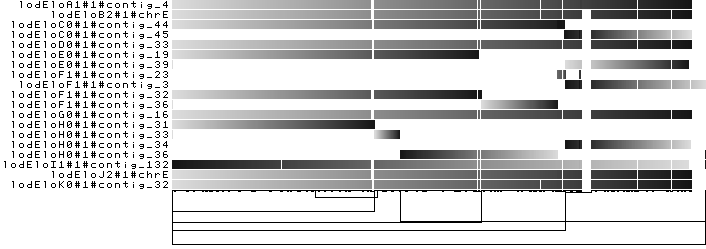
\includegraphics[width=.7\linewidth]{figures/lodelo/chrE.pggb.png}
		\caption{One dimensional visualization of the variation graph built with \pggb, containing 19 contigs from the assemblies, selected before construction using all vs all alignment data.}
		\label{fig:chrE_pggb}
	\end{subfigure}%

	\begin{subfigure}[b]{0.8\textwidth}
		\centering
		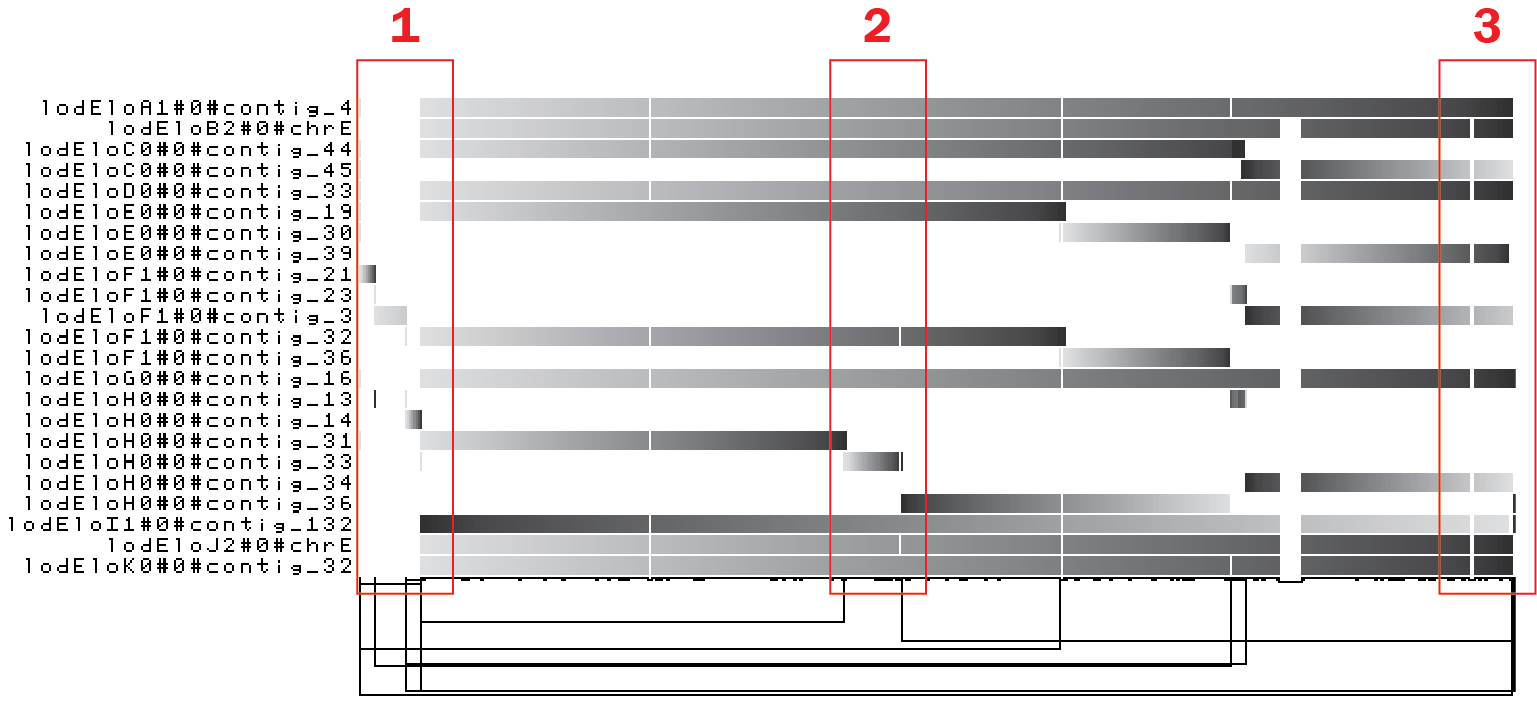
\includegraphics[width=.7\linewidth]{figures/lodelo/chrE.mcactus.png}
		\caption{One dimensional visualization of the variation graph built with \mcactus, containing 23 contigs from the assemblies, selected automatically by the pipeline.}
		\label{fig:chrE_mcactus}
	\end{subfigure}
	\caption[1D visualization of differences between \pggb and \mcactus output.]{One dimensional visualization of chromosome E variation graphs of \pggb and \mcactus using \odgi. Differences can easily be noted in the leftmost parts of the images.}
	\label{fig:chrE_difference}
\end{figure}


\printbibliography
    %\chapter{Exploring new \kmer based methods for Pangenomics} %Reducing complexity of 
\label{sec:complexity}

\section{Introduction: using \kmer sets in pangenomics}%too big, too complex, too difficult to use
As discussed in the previous section of this manuscript, the  construction of pangenome as variation graphs is based on an alignment step that is well known to be accurate but computationally expensive, even if recent advances on alignment algorithms and tools, like the wavefront algorithm~\cite{wavefront} or full-text indexes like the r-index~\cite{spumoni2} and move index~\cite{movi} have provided improvement in construction time or query performance.\\
The variation graph is a feasible approach for curated analysis of a selected set of samples for large genome organisms: for example, at the time of the writing of this manuscript the Human Pangenome Reference Consortium is releasing a second batch of around 220 high quality human genomes to be used for the construction of a new reference pangenome of the Human species.\\
Finally, the alignment step implicitly requires high quality complete assemblies to produce reasonably connected graphs. While it is expected that the availability of such high quality genomes will continue growing in the coming years, there is now available a large quantity of raw (or lightly processed) data that can be used in pangenomics applications~\cite{serratus,logan} but cannot be harnessed by variation graph models.\\ 
For this reason, \kmer based approaches provide a solid alternative: as the used \kmer length is usually relatively small (from 21 to 100), they can be used also on more fragmented assemblies or directly on raw sequencing reads and their scalability is proven to be order of magnitude superior than variation graphs. Even more so: they can be used to build representations from data of different quality like phased assemblies from one cohort and unitigs from another.\\
Such tools usually use different data structures to represent internally and in an efficient way a \dbg model. The main challenge of these data structures is mainly the amount of space used to represent the \kmers versus the time used to query elements (single \kmers or sequences). For this reason, implementations decisions are often bound to optimization compromises made to achieve a specific goal: disk compression to produce small-sized indexes from large collections; fast query time of a novel sequence; time/memory trade-offs.
In any case, the computational resources to produce \ccdbg from a set of input genomes are, as shown in the previous chapter, quite lower and the tools scale to significantly larger collections.\\
As \kmer based methods present valid alternatives for pangenomic studies, I focused part of my PhD on studying and developing data structures that could find some useful application in pangenomics. Here I will present the three projects that gave birth to some relevant outcomes.In two of these projects, I had the opportunity to collaborate with other researchers, both within my unit and from other groups.For these projects my work was included as a puzzle piece in a larger picture. While I cannot call these project as my personal contribution in the field, I believe I could bring significant input in each of them.
%As presented in the previous chapter, although using \kmer based methods for pangenomics provides the aforementioned advantages, the produced \dbg is often too big or complex to use for direct downstream applications:
%\begin{itemize}
%	\item full visualization of \dbgs for more than 10 human haplotypes is not possible with state-of-the-art computational biology tools;
%	\item when full graph visualization is possible, the repetitive regions of the genome make the graph highly connected in some parts, impeding any biological interpretation;
%	\item small region visualization is possible, usually to the scale of a gene or pseudogene, but post-processing is needed in order to polish the subgraph from parts that do not belong to the requested region, due to repetitions;
%	\item extraction of high level information is not directly possible and dependent on the construction tool: most enable presence/absence or color queries while not providing any information on where in the graph (in which unitig) the queried sequence can be found.
%\end{itemize}
%The \dbg model is therefore too complex to use for many genomic tasks, thus requiring always additional, custom scripts in order to produce information relevant for most pangenomic analyses.
The chapter will be organized as follows:
\begin{itemize}
	\item Introduction on \kmer sets and metadata representation: why it is needed and how;
	\item Overview of our contributions and my part on them;
	\item \muset: from graph to matrices for downstream analysis;
	\item Prototyping dynamic data structures for \kmer counting:
	\begin{itemize}
		\item Re-implementation of a Quotient Filter as a base for multiple applications;
		\item Explore dynamicity without indexing: super\kmer sorting;
	\end{itemize}
	\item Summary and conclusions.
\end{itemize}
%one of which is a step into providing a different representation of pangenomes as \kmer sets more suitable for downstream representation.

\section{Introduction: sets of \kmers and metadata association}
\kmer-based data structures  for representing sets of input genomes inevitably involve trade-offs to support useful applications in pangenomics.  The key characteristics of such structures are often in competition with one another, requiring a balance between the following:
\begin{itemize}
	\item Efficient storage of the data;
	\item Fast querying of a \kmer or string to retrieve its associated metadata;
\end{itemize}
The process of optimizing data storage for quick lookups is referred to as indexing, whereas the process of retrieving the metadata is called querying. Ideally, these data structures should be capable of performing both tasks efficiently, especially as datasets grow in size—as discussed in the introduction of this chapter. Given that genomic data is expanding at near-exponential rates, minimizing both storage requirements and query times for \kmer sets has become increasingly crucial.\\
A simple but very effective analogy of indexing and querying can be done with books and words.
Let's say I remember I have a book in my library that happens to have as main character someone called Ricardo and that tells about a story that is also based in Paris. Without any organization of my library I might need to sequentially read , in the worst case, all my books from start to finish to then find the one that I was looking for. This is not convenient at all, especially if I posses a lot of books. In case I maintained an index of in which book I can find any of the words from my whole library, I could quite rapidly find the few ones that contain a character that get called Ricardito. Even more, if I had also an index that associates places with books that have scenes based in them, I could easily triangulate, without even needing to open a single book, that the one I was looking for is \emph{Travesuras de la niña mala} of the Nobel Price  Mario Vargas Llosa.
This is an example of how, indexing sequencing data, \emph{the words} and their metadata, \emph{the places}, one can rapidly check which samples, \emph{the books}, contain a requested value, without having to look at the raw data (the content of the book).\\
As the \dbg is a model for a \kmer set representation, under the hood there are different data structures that can be used to store the \kmers and index them for efficient retrieval. These data structures can be divided into exact and inexact data structures. In the rest of this section I will present the characteristics of such data structures and briefly mention some propaedeutical to the prototypes we developed.

\subsection{Hashing \kmers}
As described in section~\ref{sec:kmer}, a \kmer is a sub-string of length $k$ of a biological sequence. In order to reduce the space used to store them, the text string is converted, or hashed, into a binary string that can therefore be interpreted as an integer number. The use of the equivalence of a binary string with an integer is the basis of a great part of \kmer based data structures: from here on we will consider methods for \kmers representation as binary string using hash functions. Methods that consider \kmer as text string won't be therefore consider.
\begin{description}
	\item An hash function is any function that maps data from one set (usually text but not only) to another (usually fixed-size machine-word-length integers). The ingested value is called key and the output is usually called hash value or simply hash. They are used in a lot of applications such as basic computer science models like dictionaries, cryptography or bioinformatics.
	\item hash functions should optimize on some of these properties:
	\begin{itemize}
		\item[\textbf{Uniformity}] In most cases input data should be mapped in an uniform way in the output space: in the \kmer case, lexicographically similar \kmers should be mapped to different hashes. This is not true when data locality matters: the property of similar \kmers pointing to similar hashes can be used by some data structures to avoid many cache misses, improving the computation time.
		\item[\textbf{Speed}] the fastest it is possible to compute a hash from a key, the better it is. Speed depends on the number and latency of the operation executed in the computation;
		\item[\textbf{collision avoidance}] collisions, i.e. mapping different keys into the same hash, should be infrequent. The collision rate is proportional to the size of the hash space and therefore to the space that can be used to store the hash. This trade-off will be explored better in the next section.
	\end{itemize}
\end{description}
Moreover, \kmer length impacts the time/space trade-off stated in the previous section: as larger \kmer offer greater specificity, they largely increase the amount of space needed to store them (because the hash will probably be larger) as also shown for plain-text representation in section~\ref{sec:kmer}.

\subsection{Minimum set of operations and metadata}
Given a set of sequencing samples, the data structure should support the addition of k-mers from each sample through an \emph{insert()}  operation during its construction. In some data structures, the order of the input data doesn't matter, while others require a specific order for insertion to function correctly. As we'll discuss in more detail in Section \ref{sec:staticdynamic}, post-construction insertion isn't always a guaranteed feature in certain implementations.\\
Normally these data structure can return two kind of information: the presence absence of an element, using a \memb operation and metadata associated with the specific \kmer. There are some implementations in which:
\begin{itemize}
	\item only the presence or absence can be retrieved, using the \memb operation. Bloom-filters, that will be presented in section~\ref{sec:bloom_filters}, fall under this category.
	\item only metadata can be retrieved. Minimal Pefect Hash Functions (MPHF), that won't be discussed in this manuscript, are maps of a static set of known keys to metadata that do not support \memb operations~\cite{mphf}.
	\item both presence and metadata can be queried, like color compacted \dbg, presented in section~\ref{sec:ccdbg}.
\end{itemize}
Metadata is a broad keyword that I will use to identify information associated to the \kmers represented in the data structure itself. Presence or absence of a \kmer in the set is usually, with some exception like \gls{MPHF}, directly encoded in the insertion of the elements in the data structure and do not require additional bits. Data structures that report only absence or presence are considered to not support metadata. The ones that do support different kind of metadata are considered associative, i.e. associate metadata to the \kmers.\\
A data structure may or may not retain internal information after executing a membership query. For instance, when searching for an element in a dictionary, the CPU ends up accessing a chunk of memory that includes the queried key-value pair along with other closely located data. Some data structures explicitly store variables to remember exactly where in their internal representation the most recent \memb operation occurred. This becomes especially important when sequences, not individual \kmers, are queried, as sequential \memb operations are performed on \kmers that typically overlap. Efficiently leveraging these properties can significantly impact the scalability and performance of these data structures.

\subsubsection{Metadata types}
The most trivial case it is presence of the absence of an element inside it, using a binary \memb operation (0 for no, 1 for yes). Other metadata that can be useful in pangenomics can be:
\begin{itemize}
	\item[\textbf{count}] If the data structure contains the number of times a \kmer has been seen in the input sample, the \memb operation will return 0 if it has never been seen, and a value $>= 1$ if the value has been seen 1 or multiple times. The count can be exact or represent an order of magnitude of the counts: this is often needed to not saturate the counts as most datasets have skewed \kmer count distribution. Counts are useful to discern copy variants number in different samples.
	\item[\textbf{colors}] In the case it remembers in which samples a \kmer has been seen, the \memb operation will return a list of containing samples for each queried \kmer. 
	\item[\textbf{Id}] In applications in which the graph structure is relevant (for example in visualization), it is useful to know in which \kmers (in the case of \dbg) or unitigs (in the case of \cdbg) of the graph it is contained the queried sequence. This case is relevant for \dbg based models.
	\item[\textbf{Text}] Text data can be used to associate \kmers to genetic information as genes, regulatory elements, flags to discern pathogenic variants from non-pathogenic ones and so on.
\end{itemize}
Of these metadata, the first two are the ones that are usually taken in consideration for query by recently developed data structures. Text data would impose a significant space requirement for the data and could be mimicked by assigning numerical labels to text and use an additional map to report the text for the \memb operation. The id information is quite overlooked by, to my knowledge, all implementations.\\
Finally, the main difference between representation of \kmer sets and sets of \kmer sets is that in the second each input sample is considered as a different set. This is done by using colors, that make possible to retrieve from the data structure in which sample a \kmer can be found. The color terminology can be confusing as it is often used to refer to two different concepts. From here on, the term color is used to refer to the data set from which a set of \kmer comes from. A \kmer $x$ will have colors 1,2,3 if it comes from dataset 1,2,3. As in practical cases most \kmers are divided into subgroups that contain the same colors, sometimes \kmers are associated to color sets, that represent a specific group of colors. For example the color set A will contain colors 1,2,3 so in the data structure \kmer $x$ is associated to the identifier A and the dataset of origins can be retrieved by remembering the map from color-set to colors. The use of color sets instead of directly associate a \kmer with its colors allows efficient storage\cite{ggcat}. 

\subsubsection{Metadata: why it is important}
Metadata is important to enable different kind of applications that need more information than just the presence or absence of a \kmer in a set. \\
In some applications, it's important to understand how many times a particular genetic sequence is repeated, and \kmer counting can serve as a useful proxy for that. For instance, the abundance of specific RNA molecules in a cell can help differentiate between normal and cancerous activity~\cite{kamrat,transipedia}. Similarly, variations in the copy number of specific \gls{DNA} regions can distinguish between phenotypes, revealing important differences between samples in a pangenome. In \dbg models, counting \kmers is essential to capture the multiplicity of repeated sequences, whereas in variation graphs, copy number variants are implicitly represented within the paths themselves.\\
In some applications it is important to discern between the different samples used to fill the data structure, hence representing sets of \kmer sets~\cite{metadbg}. Colors are vastly used in pangenomics, as they allow to keep track of the genomes associated to variations and the ones that are part of the core genome, both in bacteria and in eukaryotes.\\
Remembering the \dbg overlap structure is also important in many applications that rely on visualization. This would enable fast subgraph identification for loci of interest and enable specific genomic applications for \dbg based methods. For example \ssh, an indexing data structure for unitigs, would be suited for this scope~\cite{sshash}.\\
Finally, part or all of these these metadata might be useful to be stored at the same time for many applications, including pangenomics. For example, \kmer counts and colors are necessary at the same time to enable lossless encoding of genomes in a \dbg model (but they are not sufficient).
%The result of the \memb operation can be exact or approximate, i.e. have false positives. 

\subsection{Basic data structures: sorted list and hash table}
The most basic data structure used in computer science to maintain an ordered collection of elements for efficient searching is a sorted list. By ordering the entire enumeration of the set of \kmers in each sample, one can use a binary search algorithm to find a requested \kmer in time $O$($k$log$n$), using $O$($kn$) space. The use of sorted lists for \kmer storage and retrieval is feasible for very basic cases involving small sets of \kmers. However, this approach becomes intractable for the large-scale genomic applications previously mentioned, due to poor scaling in both query time and storage requirements. Nevertheless, sorted list can be used in case the number of elements is greatly reduced (by using compacted \kmer representations for example) and to avoid costly indexing. More on sorted lists is going to be discussed in section~\ref{sec:skmers}.\\
Hash-tables, a well known implementation of dictionaries (or maps) in computer science, associate keys and values using hash functions. Hash tables solve the problem of the query time, bringing it to $O$($k$) or $O$(1), depending on the particular hash function used. As they still require $O(kn)$ space, general hash table implementations can be used when dynamicity is required and the space (bit per \kmer) is not a major bottleneck: Rust HashSet implementation has shown to be useful in particular genomic use-cases, as to find in which reads are present \kmers belonging to a specific set. I provided a small contribution on this particular subject by helping with the development of Back to Sequences, a tool written in Rust that uses an hash table to find in a set of samples $S$ the reads $r$ containing \kmers present in a set $K$. The tool outputs the sequences containing the \kmers, using both a minimum and maximum threshold given as input~\cite{back_to_sequences}.\\

\subsection{Approximate membership and filters}
Approximate Membership Query (AMQ) data structures offer a trade-off between storage space (in memory or on disk) and query accuracy to enhance space efficiency. Unlike sorted lists or hash tables that always return correct information, AMQ structures respond with a non-zero probability of false positives (i.e., reporting the presence of an element that is not actually in the dataset). Due to this probabilistic nature, they are often referred to as probabilistic data structures.\\
Filters are a subset of AMQs frequently used in genomic applications. They allow fast answers on negative queries. Their basic element can be either a single bit (hence bitvectors) or any amount of bits that ensure optimal space-efficiency. These 'slots' that contain data can be smaller than a machine word or a single byte, using low-level implementation operations.

\subsubsection{Bloom Filters}
\label{sec:bloom_filters}
Bloom filters are the most used probabilistic data structures and are used in a multitude of genomic applications, like removing from ancient DNA~\cite{akmerbroom} or non-genomic applications (non-genomic bloom filter). They are used to provide a very space-efficient representation of a set of \kmers by using a bitvector and multiple different hash functions. When an \kmer is inserted, multiple different hashes are generated and the position in the bitvector corresponding to the hashes are set to 1. When an element is queried, the same hash functions are applied and if all positions in the bitvector are set to 1 the element is considered present. If at least one position is set to 0 it means that the element is not present, thus preventing false negatives. As collision can happen, especially when using multiple hash functions, it is instead possible that a position associated to the output of a hash function of a \kmer was set to 1 by the output of another hash of another \kmer, leading to false positives, i.e. reporting a \kmer is inside the data structure while it is not present.\\
Counting bloom filters store counts instead of presence/absence in the vector positions. The value they return depends in the way elements are inserted. A \kmer count gets updated if a value larger than the stored one gets inserted. When a sequence is queried, they return the minimum value of the counts associated to the composing \kmers.\\
Interleaved bloom filters are instead made of several bloom filters, as each one is filled with \kmers from a specific sample. The filters are divided into chunks and each specific chunk of all filters can be found in a contiguous region of memory. This speeds up color queries, as the lookup is done in a specific constrained region, limiting cache loading or misses.\\
Multiple implementation and optimization techniques, like the blocked-bloom filters used to speed query and insert operations, are used to maximize the potential of this data structure won't be addressed here but are thoroughly explained in these reviews~\cite{marchet2024kmersets,marchet2021kmer,marchet2024coloredkmersets}. 

\subsubsection{Quotient Filters}
Quotient filters are another data structure that is based on the idea of filling a vector with metadata but it does so in a different way compared to the bloom filter.
The hash computed from the \kmer get separated into two parts: the quotient (leftmost or rightmost bits, depending on the implementation) and the remainder (the rest). The size of the quotient depends on the amount of data that is being stored. Instead of filling the vector with the metadata at the position associated to the whole hash, it fills the slot at the position associated with the quotient with the remainder. In order to avoid collision when hashes with the same quotient occur, the remainders of a quotient are stored in order in successive slots, also called runs, to preserve the information and enable fast queries. This is done by using companion data structures that are used to trace where the run of a quotient is in the vector. When metadata that is not absence or presence has to be stored, like counts, multiple slots can be used to encode the count of a single remainder, like for the Counting Quotient Filter or some bits of the slot might be reserved to store the count, like in the Backpack Quotient Filter.
These filters enable collision resolution by using slots in a more flexible way. More about this data structure will be discussed in section~\ref{sec:qf}.

\subsection{Static vs Dynamic data structures}
\label{sec:staticdynamic}
Another important feature of \kmer data structures is whether they can be modified after construction, which brings us to the distinction between static and dynamic data structures.\\
\begin{itemize}
	\item \textbf{Static data structures} cannot be altered once they have been built.  Addition or removal of elements from the original set is not supported. To modify the underlying set, the entire data structure has to be recreated. Their advantage is efficiency, as they usually allow for greater compression and use less space making them ideal for applications where a stable reference set is used, and there isn’t a need for frequent modifications. For example, they’re well-suited for comparing new datasets against a reference genome that remains constant.
	\item \textbf{Dynamic data structures} allow updates after their initial construction. The types of modifications that can be made depend on the specific implementation and the use case. The most common operation is the insertion of new \kmers, which effectively functions like a union of two sets (for presence or colors). In the case of counting structures, usually a count of an existing \kmer is updated if last inserted has a greater count. Other possible updates include deleting \kmers or modifying the metadata associated with them.
\end{itemize}
While most methods are static, dynamic structures that allow efficient insertion and, less frequently, deletion of \kmers are being developed in recent years~\cite{marchet2024kmersets}.

\section{Our contributions: an outline}
The three projects span different topics and can be devised at 2 different levels of engineering. The first is mainly organizing a pipeline with some already developed bioinformatics tools and contributing to the development of a tool for \kmer information manipulation. The other two are development of a tool from scratch.\\
They can be presented as follow:
\begin{itemize}
	\item[\textbf{\muset}] is a pipeline to construct plain text unitig matrices from input sample. It enables to build an abundance matrix in which the unitig count in each sample is the average of the counts of its constituent \kmers and a presence/absence matrix that report an unitig as present in a sample if its constituent \kmers are present in the sample over a given threshold.\\
	\item[\smash{\stackunder{A \textbf{Quotient}}{\textbf{filter}}}] implementation that allows dynamic updates, resizing, and a framework to develop different specific data structures on top of it. It is the building block of a novel data structure, the Backpack Quotient Filter that has been recently published. I also redeveloped a Counting Quotient filter on top of it with a \emph{Fimpera} scheme to mimic large \kmers while store smaller ones to store space.\\ 
	\item[\smash{\stackunder{A \textbf{Super\kmer}}{\textbf{sorting}}}] implementation to explore a different data structure to store \kmers without indexing and allowing queries.
\end{itemize}
Some of the research and development I did, mostly in the second and third projects, can be labeled as exploration and prototyping as the result is not intended to be a novel tool to be widely adopted by the community but as first step in possible route of research in this domain.

\section{\muset: building unitig matrices for downstream analyses}
In this section I will present the work that I have been doing on building unitig abundance matrices.
\subsection{Rationale}
Recent advancements in genomic sequencing technologies have led to the generation of massive datasets from large-scale projects. Some of them very functional to human pangenomics, such as the 1K Genomes Project and the HPRC, while others focus on related genomic areas like transcriptomics (e.g., GEUVADIS) and metagenomics (e.g.,MetaSub, Tara Ocean).\\
In pangenomics, these large datasets present significant challenges for traditional variation graph analyses due to their size and complexity. \kmer-based methods offer an alternative approach to study this data, using techniques such as \kmer counting and matrix representation. These methods can lead to improved accuracy in estimating the abundance of loci across multiple samples, enabling more comprehensive analyses of complex genomic datasets. A potential application of these methods could allow GWAS studies to be conducted on all possible variations within genomes, expanding beyond the current focus on SNPs and small indels. Additionally, \kmer abundance matrices could serve as training data for Deep Learning models to, potentially uncovering traits that distinguish healthy from non-healthy populations for specific diseases.\\
Given the usefulness of these applications, we propose a novel method for constructing plain text abundance unitig matrices. These matrices can be directly utilized in various downstream applications, offering a valuable resource for researchers in genomics and related fields.

\subsection{Related work}
Cutting-edge tools that compute a \cdbg or \ccdbgs form input samples have been developed in recent years. While \bcalm and \cuttlefish output a \cdbg (hence a \kmer set) that do not record the sample of origin, \bifrost and \ggcat do build \ccdbgs that use colors to trace the source of the \kmers. While \ccdbgs are an implicit representation of an unitig matrix, as they contain the same information (unitigs and origin of \kmers) but represented in a different way, tools that build them do not produce a matrix as output nor provide any APIs or scripts to do so.\\
Recently, \kmt~\cite{kmtricks}, a very fast tool to build a \kmer abundance matrix from a set of samples has been proposed but the cardinality of the \kmer set obtained from input data renders these matrices poorly tractable for the aforementioned downstream applications. This is not a limitation of the tool but a feature of the \kmer spectrum of the datasets.\\
Remembering that unitigs, as described in section~\ref{sec:kmerobjects}, are a more succinct representation for \kmers, we propose a pipeline that mix the strength of both \cdbg tools to build unitigs and \kmt to represent \kmer color and abundance to produce unitig matrices that are more tractable for analysis. We also propose a simple pipeline to build presence absence unitig matrices from samples using a script that renders in a digestible text format the implicit representation of a \ccdbg.
\subsection{From sequencing data to unitig matrices}
\subsubsection{Main features and differences of unitig matrices}
The construction of an abundance unitig matrix is based on two key observations: first, \kmer matrices can now be constructed with high efficiency, and second, unitigs can also be built efficiently. Therefore we can create a more compact and manageable representation that preserves the high-level information crucial for genomic variation diversity studies, loci variation visualization, and input for machine learning libraries.\\
The main parts of the process to generate an abundance unitig matrix from an abundance \kmer matrix involves compacting \kmers into unitigs and estimating unitig abundance by averaging \kmer counts. In this way we obtain a more condensed, lossy representation of the data. As single \kmer counts are lost, the essential information is preserved by the average count of the unitig. The loss of information is acceptable as the compaction provides a more computationally manageable representation.\\
In cases where abundance information is not required, presence-absence unitig matrices can be used instead. They still capture sequence variation between individuals and are valuable for diversity studies.\\
A key difference between the proposed model for abundance or presence-absence matrix construction process is a filtering step that retains only \kmers reflecting differences between samples. This targeted approach focuses on the most informative genomic regions and is applied on the abundance matrix construction. The presence-absence matrix includes the entire set of \kmers from the input genomes, providing a comprehensive view of the input data.\\

\subsubsection{Matrix construction overview}
Formally, given an unitig $u$ searched in a sample $S$, the \kmer presence ratio is defined as follow:

\begin{equation}
	f(u, S) = \frac{\sum_{i=1}^{N}{x_i}}{N}
\end{equation}

while the average abundance of a unitig $u$ with respect to a sample $S$ is defined as:

\begin{equation}
	A(u, S) = \frac{\sum_{i=1}^{N}{c_i}}{N}
\end{equation}
In the equations $N$ is the number of \kmers in $u$, and $x_i$ is a binary variable that is $1$ when the $i$-th \kmer is present in sample $S$ and $0$ otherwise, while $c_i$ is a non-negative integer count.\\
Figure~\ref{fig:muset} shows the main steps of the \muset pipeline. To produce an abundance matrix, the main steps are:
\begin{enumerate}
	\item A \kmer abundance matrix is built from FASTA/FASTQ files using \kmt;
	\item \kmers that are present in at least 10\% of the samples and absent in at least 10\% of them are retained, while the others are discarded. The thresholds are customizable;
	\item Unitigs are created from this set of retained \kmers in order to compress the representation. Unitigs shorter than a certain value are discarded. While this variable can be modified by the user, our recommendation is to keep it as $2k-1$ with $k$ the length of the \kmer. This value is the minimum value to observe a SNP in the set as an unitig representing a SNP would have 2 times $k-1$ bases as overlap to the unitigs representing the adjacent bases in the genome and 1 base for the variation.
	\item The abundance unitig matrix is therefore constructed. This is done by 
	\begin{enumerate}
		\item creating a dictionary, using \ssh, to link \kmers to the unitig in which they have been compacted;
		\item each unitig abundance score is computed by summing the count of its constituent \kmer set divided by the cardinality of the set. This is done independently for each sample to retain the color information of the \kmer matrix.
	\end{enumerate} 
\end{enumerate}
To generate a presence-absence the main steps of the pipeline are:
\begin{enumerate}
	\item unitig matrix the \ccdbg is built using \ggcat. Unitigs are in FASTA format while colors are in a compress representation accessible only via \ggcat cli or APIs.
	\item unitigs are filtered by length like in step 3 of the abundance pipeline;
	\item filtered unitigs are queried against the \ggcat color index and for each sample in which at least 1 \kmer of the unitig was present, the presence ratio is reported. If no \kmer was present in the sample, the sample is not reported.
	\item the unitig query is then parsed (from jsonl) and the presence (1) or absence (0) is reported for every unitig in every sample in form of a matrix. The presence is determined when the fraction of present \kmers in the sample is above a pre-defined, although modifiable, threshold. It is also possible to produce a matrix that does report the presence ratio instead of a binary value.
\end{enumerate}
Only the abundance pipeline has been tested against the most similar state-of-the art tool that is in fact \ggcat, that produces, as mentioned, an implicit presence/absence matrix. Even without using the just presented script to produce an explicit one, the abundance matrix script is faster than \ggcat when run on a large collection of 360 ancient oral samples, as shown in table~\ref{tab:muset_comparison}. No computational resources test has been done on human genomes as it was out of the scope of the pure demonstration of the usability and efficiency of the method. 

\begin{table}[!t]
	\centering
	%\tabcolsep=2Spt
	\begin{tabular}{lccc}
		\toprule
		Method & Wall-clock time & Peak memory & Disk usage \\
		\midrule
		\muset & \textbf{9h 43m 12s} & \textbf{\SI[detect-weight=true]{19}{\textbf{\giga\byte}}} & \textbf{\SI[detect-weight=true]{1.5}{\textbf{\tera\byte}}}\\
		\ggcat & 24h 20m 40s & \SI{167}{\giga\byte} & \SI{641}{\giga\byte} \\
		\bottomrule
	\end{tabular}
	\caption{Comparison of running time, peak memory, and disk usage between \muset (filtered unitig matrix) and \ggcat (implicit and unfiltered unitigs) on 360 ancient oral samples.}\label{tab:muset_comparison}
\end{table}

\begin{figure}[h!]
	\centering
	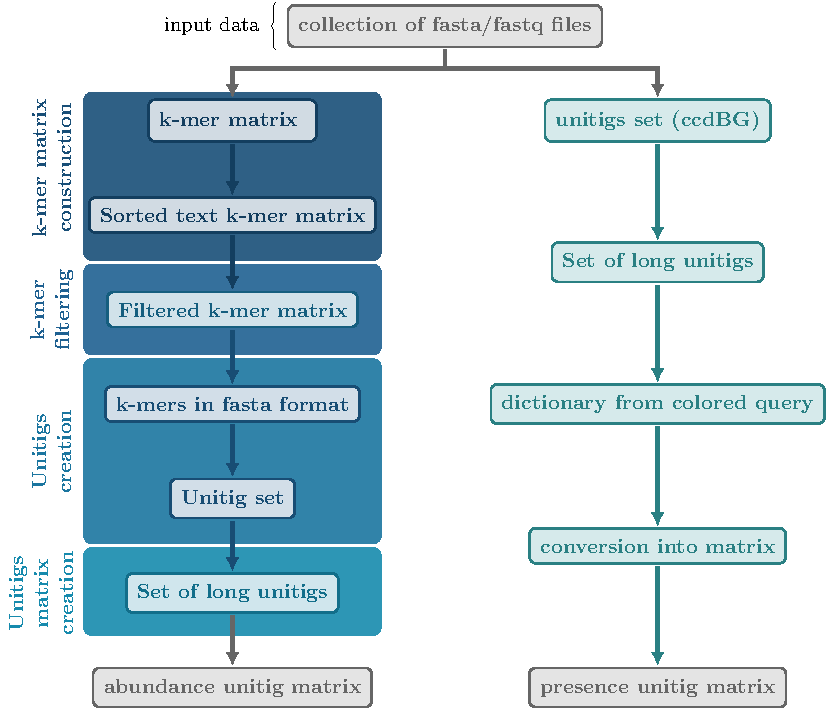
\includegraphics[width=\linewidth]{figures/kmer_methods/muset_full.pdf}
	\caption[The \muset pipeline]{Scheme representing the main steps of the \muset pipeline.}
	\label{fig:muset}
\end{figure}

\subsection{Conclusions and perspectives}
\subsubsection{Unitig matrices are pangenomes}
Matrices, although often overlooked in the pangenome community, offer a valid and valuable representation of pangenomes. Each genome can be conceptualized as a binary vector within a matrix that encodes the alleles of a pangenome graph. Both variation graphs and \ccdbgs can be used to infer presence-absence matrices, where rows represent node IDs and columns represent input samples. 
While plain text matrices may not provide the same visual representation of genome variations as graphs do, they offer distinct advantages:
\begin{enumerate}
	\item They are a more accessible starting point for downstream applications that \dbgs;
	\item bio-statistical methods and population genetics can be easily applied to this model;
	\item provide a standardized format that can be compatible with various computational tools and libraries, providing a more reliable framework for researchers to build upon. This is in distinct contrast to color representation for \ccdbgs that depend on the particular implementation.
\end{enumerate} 
The significance of \muset lies in its novel approach to generate plain text unitig matrices. Prior to the development of the \muset pipeline, abundance matrices could be theoretically generated only from paths in variation graphs. Our tool makes now possible to obtain a sufficiently precise and compact representation that enables new kind of analysis in pangenomics, transcriptomics, paleogenomics and metagenomics.\\
\subsection{Improving the method}
\muset is the first pipeline that integrates various existing and novel tools to produce unitig matrix representations of pangenomes. The \kmat software has been specifically developed for the pipeline: it implements filtering, count averaging, presence-absence steps and handles the various input/outputs. Most of the tools incorporated in \muset were instead not originally designed for this particular application.\\
While \muset's main contribution is in proposing for the first time a method to build such matrices, the current implementation has room for improvement and optimization.
The pipeline involves multiple steps in which data is written and read to disk, not for a specific design choice to ease the burden from in-memory processing, but because of subsequent steps are done by different software. Other operations are also slowing down the pipeline. Two of these that are easy to spot are: building unitigs from a file containing one \kmer per sequence in the abundance pipeline and transforming the jsonl output of \ggcat to a csv instead of using \ggcat apis to get presence values to avoid two I/O operations and dumping directly to disk the csv matrix in the presence-absence implementation.\\
Addressing these bottlenecks could yield a more optimized method to generate abundance unitig matrices that could scale to larger datasets and allow matrix-based analysis on them.
%Another, more simple, upgrade of muset would be to produce such matrices also from a variation graph to allow 

\section{Prototyping Dynamic Data structures for \kmer counting: a Rank Select Quotient Filter}
\label{sec:qf}
While abundance unitig matrices are valuable for specific genomics applications, they may not be the most efficient representation for all use-cases. In particular, some applications require rapid determination of presence or absence of specific sequences in datasets of interest. By indexing the dataset, the information is organized in data structures that enable fast data queries.\\
Sequence query in \kmer based data structures is typically performed through pseudo-alignment, a technique that involves tokenizing sequences into \kmers and querying each of them. Some data structures exploit the difference of just 1 character between subsequent \kmers to query to rapidly query multiple of them. While \cdbg or \ccdbg can be used to address this task, the graph construction is a major bottleneck and requires explicit association between each \kmer and its abundance. \\
\subsection{Brief filter data structures overview}
\kmer storing data structures imply mainly two strategies to efficiently store and retrieve them: representing \kmers as string or as hashes\cite{marchet2024kmersets}. In this work we will describe a method that stores \kmers as hashes and in particular uses structures with false positive rates. Other hash-based data structures are static or dynamic hash tables~\cite{sshash}.\\
Approximate Membership Query (AMQ) data structures, such as Bloom filters, quotient filters, and cuckoo filters, offer a more space-efficient representation of a set or multi set of elements. These data structures have become essential tools not only in computational biology but also in other domains like databases, storage systems and networks. They are termed approximate because they allow queries to return a controlled false positive value at a rate $\delta$. This means that while they always confirm the presence of an inserted item, they might erroneously return true for non-inserted items with a probability of $\delta$. This trade-off provides space savings.\\
Recent developments in the \kmer field yielded improved version of data structures that allow to store the count of elements in a dataset, instead of just reporting the absence or presence~\cite{squeakr,pandey,cqf,comin_count,sshash}. AMQs that provide this feature are termed counting AMQ or cAMQ. In the case of cAMQ, false positive values should report a count greater and not inferior to the real ones: this means that they should never underestimate the abundance of an element in the dataset. These data structures are particularly useful in many bioinformatics applications, from pangenomics to transcriptomics and metagenomics.\\
At the present moment, the main areas of improvement of such data structures are:
\begin{enumerate}
	\item latency of \memb operations. It determines the range of applications they can be used for (e.g., computer networks) and the volume of data that can be queried within a reasonable amount of time (e.g., bioinformatics). The latency is mainly influenced by:
	\begin{itemize}
		\item data locality design. Developing an architecture that reduces cache misses by storing data that might be frequently accessed together in slots that fit within the largest process cache.
		\item implementation efficiency, by carefully engineering the software for code branches, SIMD operations and multiprocessing. This is aspect is particularly important, as theoretically less efficient data structures can outperform others in practice due to optimization.
	\end{itemize}
	\item space efficiency, as it poses constraints on the computer architectures that can utilize it. Despite RAM cost declining, the more rapid growth of data requires efficient and parsimonious encoding of data to the bit level.
	\item operation range. The possibility to modify the data contained after initialization. The most useful operations are:
	\begin{itemize}
		\item incrementing elements count, or add new ones; 
		\item decrementing elements count, or removing them when their count reaches zero;
		\item enumerating elements with their respective count;
		\item automatically resize the filter when it reaches maximum capacity, avoiding the need for a priori cardinality estimation and allowing for addition of new elements.
	\end{itemize}
\end{enumerate}
A data structure that addresses efficiently all these aspects is the Counting Quotient Filter or CQF. It is based on the Rank-Select quotient filter and it uses a counting scheme to efficiently encode the count of inserted elements in the slots of the filter. This method offers reduced memory usage and faster lookup speed compared to inserting multiple times elements in a Quotient Filter to remember the counts.
\subsubsection{Filter data structures}
AMQs are often termed with the name of filter. Here I briefly describe the most common ones.
\begin{itemize}
	\item[The \textbf{Bloom filter}] is a well-known AMQ, which uses hash functions to map inserted items into a bit vector. Despite its space efficiency (one to two bytes per element for common $\delta$ values like 1/50 to 1/1000), a major drawback is it cannot be resized and doesn't support deletions. Counting Bloom filters (CBF) extend Bloom filters by using saturating counters instead of bits, enabling deletions at the cost of increased space. Scalable Bloom filters, on the other hand, maintain a low false-positive rate even when the number of items is unknown by employing multiple Bloom filters.
	\item[The \textbf{Quotient filter}] uses hashed fingerprints to manage table slots. It supports a range of operations like insertion, deletion, and resizing. It is more cache-efficient and faster than Bloom filters—though less space-efficient than CBFs—making it suitable for systems like SSDs. One downside is that its performance degrades significantly once the table exceeds 60\% occupancy.
	\item[The \textbf{Cuckoo filter}] uses cuckoo hashing. It uses two potential slots for storing each item and moves items between their alternate locations if needed, causing a cascade of movements (kicks) until a stable arrangement is achieved. This filter is fast for loockups but can suffer from poor cache performance if many kicks occur, especially when the structure becomes full.
\end{itemize}
All these implementations provide a fast lookup table where information can be stored in fixed-size slots.\\
I will focus on the implementation of the Quotient Filter, as it forms the basis of our implementation.

\subsection{Quotient Filter structure: Rank and Select}
The Rank-Select quotient filter, or RSQF, works by hashing items into a $p$-bit fingerprint $x$ and then dividing the bits into two parts: the quotient $h0(x)$ of $q$ bits and the remainder $h1(x)$ of $r = p - q$ bits. The RSQF has an array of $2^q$ $r$-bit slots that store the remainder of each item. When inserting an item, the process begins by attempting to place the remainder in the slot determined by the quotient. If the home slot is occupied, a linear probing technique is used to locate the next available slot.
To track and manage the runs (collections of subsequent slots containing remainders of a specific quotient), the the RSQF uses two metadata bitvectors:
\begin{itemize}
	\item[occupieds] it tracks which slots are currently occupied by data;
	\item[runends] indicates the end of each set of consecutive entries (or a "run") in the quotient filter.
\end{itemize}
The combination of these two bit vectors allows the RSQF to efficiently locate and manage inserted items by using rank and select operations. Specifically, the \texttt{RANK} function counts the number of occupied slots up to a certain point, and  \texttt{SELECT} identifies where in the filter a particular run ends. This allows efficient lookup, insertion, and enumeration of the data in the filter.\\
Moreover, to store the data in a cache-friendly way, the filter is structured into blocks of 64 slots. To minimize operations requiring the scan of multiple blocks when the filter is relatively full, an offsets array tracks the distance from the start of a run to where it ends, every 64 slot. Computing offsets involves scanning only small sections of the metadata (64 bits or fewer) per operation, making the filter significantly faster.\\
Each block fragments contains one offset value, 64 occupieds bits, 64 runends bits, and 64 slots for remainders data. By grouping these elements together, the system minimizes memory access and enhances cache efficiency. This structure is optimized for rapid traversal and manipulation of the filter content to enable fast membership queries and updates.\\
A scheme of how the quotient filter works is shown in figure~\ref{fig:qf_ex}. For the sake of simplicity the metadata vectors are not shown.
\begin{figure}[h!]
	\centering
	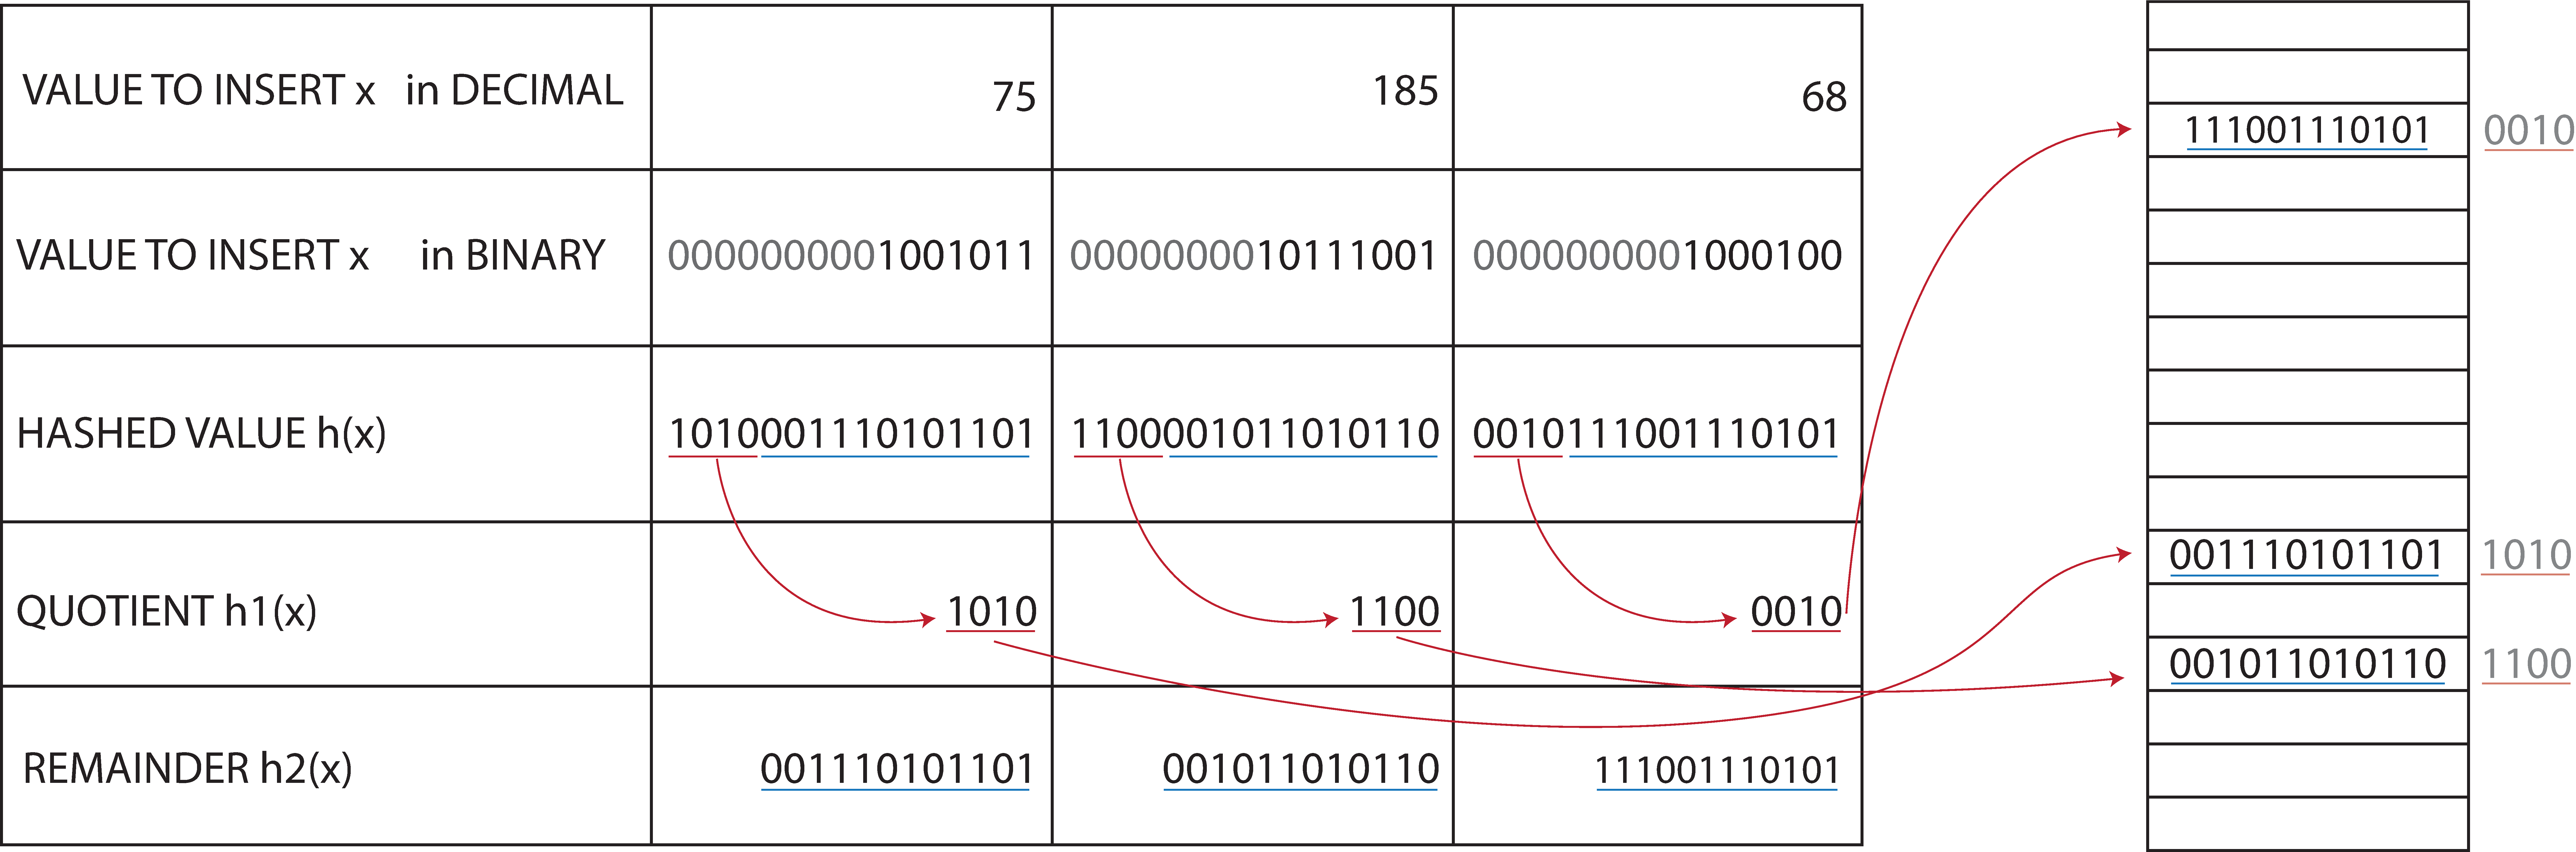
\includegraphics[width=.95\linewidth]{figures/kmer_methods/quotient_filter_export.pdf}
	\caption[Example of a quotient filter.]{Example of a quotient filter.An integer, represented in decimal form, can be expressed as a binary sequence. An unsigned 16-bit integer is composed of 16 binary digits (bits) that can store a value from $0$ to $2^{16}-1 = 65535$. To construct a quotient filter, a hash value is generated by applying some binary operations on this integer. From the computed hash value, the leftmost 4 bits are considered the quotient (although, depending on the implementation, the rightmost bits could be used instead). The remaining bits from the hash form the remainder. The remainder is stored in the filter at the position indicated by the quotient. }
	\label{fig:qf_ex}
\end{figure}
\subsubsection{Counting}
\label{sec:rsqfcount}
Counting data structures can store either exact counts or order of magnitude, depending on the application. In fields like human genomics, where count numbers are expected to be relatively low and precision is crucial, exact counts are preferred. Differently, in fields like metagenomics, where skewed abundance is more probable, an estimate of the count is often sufficient.\\
Counts can be stored using three different strategies. In all cases, the reminders associated with a certain quotient are stored in monotonic order within the data structure.
\begin{enumerate}
	\item  a count can be encoded as the number of times a reminder is inserted into consecutive slots. This is the most basic implementation and in most cases the least space-efficient one. The data structure occupation is directly related to the total number of counts in it, making poor use of the bits in the slots.
	\item a count $N$ of a reminder $R$ can be encoded into multiple consecutive slots as follows: 
	\begin{itemize}
		\item if $1 <= N <= 2$, than the reminder $R$ is inserted $N$ times;
		\item else $K = C - 2$ can be encoded into a sequence of slots. The boundaries are flagged by two remainders $R$. The slots in between store the count $K$. To signal that the slots are used as counter, the count elements break the monotonicity just after the first remainder.
		%The encoding uses the slots in between to store the actual value of the count $K$. If $K$ is greater than $R$, a 0 is placed just after the first reminder to signal that the next slots are used for encoding, else not as the monotonic insertion of the reminders would implicitly flag the count. If $K$ is greater than the max value that can be encoded in the $r$ bits of a slot (i.e. $2^r -1$), it is encoded as a sum of the slots containing the count. 
	\end{itemize}
	This approach uses at least 3 slots for $n>2$ and, while more efficient than the first, is still inefficient for low count values.
	\item another way of storing $c$ is reserving $m$ extra bits for every slot to encode in it the count associated to the remainder. As this method adds $2^q * c$ bits the choice of $c$ should be calibrated for the suited application. 
\end{enumerate}

\subsection{Developing a new library for a Quotient Filter}
The pre-existent implementation of the CQF is efficient but has several limitations. It represents an immutable object, limiting experimentation with different models based on the Rank-Select Quotient Filter or the Counting Quotient Filter. It lacks dynamicity due to static allocation of the table and does not address issues related to the filter's toricity when accommodating new elements.
To overcome these limitations, we decided to re-implement the data structure with key improvements.\\
The new data structure explicitly manages the filter's toricity, addressing cases where the final part of the filter is filled with data and new insertions push elements to the beginning of the filter. This means that there is no logical start or end of the table, as elements can be moved from the last slot to the first as continuation of the filter.\\
It automatically resizes when reaching the imposed threshold of maximum occupancy by doubling the size of the table. This feature allows for continuous insertion of new elements.\\
It supports the enumeration of inserted elements.\\
The filter is designed in a modular structure, so that the basic RSQF data structure serves as a building block for different applications.\\
The developed data structure allows for the creation of models that are:
\begin{itemize}
	\item exact (when no space trade-off is chosen) or approximate;
	\item capable of handling exact or approximate counts;
	\item capable of handling different count encoding;
\end{itemize}
The data structure is layered as follows:
\begin{itemize}
	\item[\textbf{Low Level}] comprises agnostic operations in the data structure such as
	\begin{itemize}
		\item setting a specific slot to a certain value. The value can be a remainder, count or combination of the two. It can also be any metadata as it only imposes bits to a certain region of memory corresponding to a slot;
		\item clearing of a slot to zeros for removals of elements from the filter and shifting operations;
		\item reading the value from specific slots;
		\item shifting slots by a certain amount $z$. Slots starting at position $x$ to $y$ are moved between positions $x+z$ and $y+z$ modulo the length of the filter. This operation is needed when a new element has to be inserted in an already occupied position. By shifting right of $z$ slots the already set slots, the position $x$ to $x+z-1$ are therefore free to accommodate new elements or counts;
		\item metadata operations for setting to 1 or to 0 the occupied and runends bits in their bitvectors;
		\item updating the offset vector to track of runs.
	\end{itemize}
	\item[\textbf{Medium Level}] it comprises operation to insert,removing and querying elements without explicitly caring about bit-level operations. They implement a RSQF data structure.
	\begin{itemize}
		\item addition of an element to the data structure;
		\item removal of an element from the data structure;
		\item query of an element from the data structure;
		\item metadata handling in each of the aforementioned operations.
	\end{itemize}
	\item[\textbf{High Level}] it comprises operations built on top of the RSQF layer and described a CQF.
	\begin{itemize}
		\item extended addition and removal to allow for multiple slots altogether;
		\item functions to encode and decode counters, as described in point 2 of section~\ref{sec:rsqfcount};
		\item query operations using specific linear probe, recognizing the start and end of a counter.
	\end{itemize}
	\item[\textbf{Application Specific}] functions specific for handling input, output and resize.
	\begin{itemize}
		\item \kmer hashing.
		\item initialization of the data structure;
		\item enumeration of elements within the data structure;
		\item dynamic resizing of the data structure, including element enumeration, filter size doubling, and element reinsertion;
	\end{itemize} 
\end{itemize}
This implementation has been developed as both a library and standalone software, offering flexibility in its application.
\subsubsection{Allowing multiple types of counts: CQF and BQF}
While the primary focus was on re-implementing a Counting Quotient Filter (CQF) from the Rank-Select Quotient Filter (RSQF) implementation, the basic structure with low to mid-level operations and application operations can be used to build other models on top of the RSQF. Victor Levallois has successfully implemented another data structure called the Backpack Quotient Filter (BQF), which uses the count encoding presented in point 3 of the previous section on RSQF counting methods~\ref{sec:rsqfcount}. Instead of using other slots to encode the counter, it reserves a pre-defined amount of bits in the remainder to store the approximate count:this is done at the expense of some precision~\cite{bqf}.\\
The successful implementation of the BQF demonstrates the flexibility and extensibility of the proposed architecture in order to handle different kind of counts.

\subsubsection{Handling toricity}
A crucial property of the filter, overlooked in the original CQF implementation, is the handling of specific edge cases related to its toroidal structure. Runs of reminders (or counts or combinations of both) associated with the same quotient are stored contiguously in monotonic order. This storage must be done in increasing slot ID order. When two elements with the same quotient are added to an empty filter, the slots used are the one associated with the quotient and the one \emph{on the right}(i.e., the slot associated with quotient+1), and so on.\\
A challenge arises at the \emph{rightmost} or final part of the filter. When new elements are added, it's likely that at some point, a slot should be pushed to the next element after the final slot. To address this issue, the filter is implemented with a toroidal structure, meaning the slot following the last slot is the first slot of the filter. This property eliminates problems associated with filling the filter in the final slots by imposing equal properties to all slots in the filter.\\
Implementing the filter with this characteristic is non-trivial, as the toroidal property requires different handling of all comparisons within functions and shifting operations. It necessitates careful consideration of edge cases and boundary conditions to ensure correct behavior when operations wrap around from the end to the beginning of the filter.\\
This toroidal implementation enhances the robustness and efficiency of the filter, allowing for more uniform utilization of the entire data structure and eliminating potential bottlenecks that could occur at the boundaries of a linear structure.

\subsubsection{Dynamic resizing strategy}
The proposed implementation of the filter eliminates the need for a priori computation of the \kmer set cardinality (and estimating the slots used by the counts), allowing for direct data insertion. To prevent failure when the number of inserted elements exceeds capacity, a dynamic resize and reallocation strategy is implemented. A specific counter is incremented each time a slot is used in the filter. This counter keeps track of the slot occupancy ratio: when the number of occupied slots reaches 95\%, the insertion process is paused and the resize operation is initiated. The process operates as follows: 
\begin{enumerate}
	\item Enumeration: all stored elements (with their counts) are enumerated. These are temporarily stored in a hash table, with the element as the key and the count as the value. The enumeration is done by linear probing the entire filter. Each occupied metadata bit is sequentially scanned. When a bit is set to one, the probe looks for the corresponding run of remainders in the filters and proceeds to enumerating all the elements (composed of the combination of quotient and remainder) with their counts. When the entire occupieds bitvector is scanned, the enumeration ends.
	\item Parameters update: the size of the quotient is increased of one and the size of the remainder is decreased of the same amount. By adding 1 bit to the quotient, the number of index-able and insert-able elements doubles. All other internal values depending on quotient or reminder are updated. The occupancy counter is set to 0.
	\item Re-instantiation of the vectors: the remainder vector and the metadata vectors are doubled in size.
	\item Insertion of elements in the new filter. The elements are fetched from the hash table and inserted back in the filter.
\end{enumerate}
The dynamic resizing allows for flexible use of the data structure without prior knowledge of data size and ensures efficient space utilization by growing only when necessary. However, this his process produces a temporary spike in memory, by having at the same time the map containing the enumeration and the newly doubled filter.

\subsubsection{Using the Fimpera scheme to reduce space}
The size of a RSQF data structure is given by $2^q * (r + m )$ bits, where $m\sim 2.125$ metadata bits (along with some other relatively negligible overhead). This suggests that if there were a way to store nearly the same input information while reducing $r$, it would yield substantial space savings and enable the use of the data structure on larger datasets. T To achieve this goal, both the CQF implementations has been developed also with the Fimpera scheme incorporated~\cite{fimpera}, like the BQF.

Fimpera operates by splitting each \kmer into smaller \emph{s-mers} and storing them in the filter, each with the \kmer count. The \kmer abundance can thus be retrieved through its constituent \emph{s-mers}, as the presence of a\kmer implies the presence of all its constituent \emph{s-mers}.\\
This approach has been demonstrated to significantly reduce the false-positive rate by an order of magnitude without generating false negatives or underestimating \kmer abundance~\cite{fimpera}. In this context, Fimpera is used to reduce the dimension of the filter without increasing the false-positive rate, as storing smaller hashes from \emph{s-mers} results in a smaller $r$.

To estimate the correct abundance of a \kmer, the smallest count among its constituent \emph{s-mers} is used.
The major drawback of this scheme is the loss of the \kmer enumeration feature, as only the \emph{s-mers} can be retrieved. However, the dynamic resizing of the data structure is preserved as only \emph{s-mers} are required to be remembered.

This approach may introduce false positive \kmers: \kmers that are non present in the original dataset but are composed of \emph{s-mers} found in other \kmers are going to be reported as present. As this is a joint probability, it is the produce of each independent probability, becoming very low when $s$ is sufficiently large. The $s$ parameter must be chosen as a trade-off between space efficiency and false positive rates. For the BQF, this has been estimated as under $10^{-5}\%$ with $s > 20$ when $k = 32$.

This Fimpera-enhanced implementation offers a novel approach to improving the space efficiency of RSQF-based data structures while maintaining acceptable error rates and proves the flexibility of the proposed implementation.

\subsection{Conclusions and perspectives}
The proposed implementation of a prototype quotient filter has demonstrated considerable flexibility in its approach to storing \kmer abundances. This adaptability is a key feature that sets it apart from more rigid data structures and opens up new possibilities for genomic data analysis.\\
It could also incorporate additional metadata, which would extend its functionality beyond a conventional cAMQ. For instance, color information would be greatly useful for specific pangenomics applications. However, this extension is non-trivial due to the memory-intensive nature of color storage and encoding. An interesting direction could use of Shannon coding for colors. When the filter undergoes multiple resizes, each resize operation can be used to evaluate the distribution of contained colors. The result of this evaluation could be used to inform an adaptive encoding strategy where frequently occurring colors are represented with fewer bits, while less common colors are encoded with into large values. Such an approach would optimize the space-color information trade-off dynamically.\\
Despite its new features, this implementation has not yet found its way to a standalone publication. The current CQF implementation (without Fimpera) exhibited slower performance compared to the original, more optimized version. This performance disparity highlights the challenges providing implementations with new features without impacting computational efficiency.
Nevertheless, there is value in prototyping data structures that offer greater customization potential for specific applications, as they provide guidance for the evolution of more flexible and adaptable data structures.\\
Finally, the BQF implementation, based on this RSQF model, has been presented at RECOMBseq~\cite{recombseq} conference and will be soon published in the associated journal~\cite{bqf}.

\section{Prototyping Dynamic Data structures for \kmer counting: Super\kmer sorted list}
\label{sec:skmers}
This chapter has shown that there's no one-size-fits-all approach to represent \kmers efficiently. The most suitable method depends on the specific application. When comparing two datasets, for instance, one can enumerate all \kmers for each set and store them in sorted lists. The difference between sets can then be estimated using a set metric (like the Jaccard index) that accounts for \kmer differences in the lists. This process works well with sorted lists. Sorted \kmer lists also offer a reasonably fast representation for single \kmer queries without indexing. Binary search has query time $O(log{N})$, where $N$ is the cardinality of the set.\\
While not indexing the data provides slower data structure insertion time, using sorted lists has the advantage of requiring less space. A map index has $O(1)$ time for each insertion, leading to $O(N)$ when inserting $N$ elements. Sorting a list, when data is assumed random and without any supplementary hypothesis, requires $O(Nlog{N})$ time, if comparisons are performed. Using a list instead of a more complex data structure, like the QF, provides a more compact representation of the data in memory, as the list has no overhead: it does not uses empty slots, metadata vectors and additional variables. The size of the data structure is only the size of the raw data: not external bits of information are added, even if information is gained compared to the input through the sorting.\\
Instead of storing just \kmers, an encoding can be used to group together overlapping \kmers and save space. The \kmer research community has explored several space compression by encoding them within string sets. The idea is to construct string sets that contain all enumerated \kmers and nothing else. Recent models include unitigs, eulertigs, simplitigs and super\kmers~\cite{marchet2024kmersets}.\\
We then propose a novel data structure that combines the encoding of \kmers into super\kmers for space savings and a sorted list structure for relatively quick non-indexed \kmer queries. It therefore can be termed as super\kmer sorted list.\\
Super\kmers are sequences of adjacent \kmers that share the same minimizer. They generate a partition of the \kmer set, allowing for space savings and parallelization. Although they are a string representation, they are often used in hash-based methods as they are based on hashed minimizers. Another property of using super\kmers in the sorted list is that, since consecutive \kmers are close, they can be queried together with great computation time savings. To query, the algorithm locates the super\kmer linked to the queried \kmer minimizer and checks for the \kmer within the super\kmer.\\
Implementations like \blight~\cite{blight} and \ssh~\cite{sshash} use Minimal Perfect Hash Functions (MPHF) to facilitate mapping of minimizers to their corresponding super\kmers. The problem of using MPHF is that they generate a static dictionary that cannot be updated~\cite{smsketch}, forcing the data structure to be static. By using sorted superk-mer lists, we can instead provide dynamic updates.

\subsection{Super\kmer sorted lists: Input ad output}
The super\kmer sorting algorithm we propose is part of a larger super\kmer based data structure I contributed to. For brevity, we;ll omit the full details of this structure. \\
Our algorithm takes any source of \kmers and processes it to produce an enumeration of super\kmers that are then sorted into a list for efficient lookup.\\
While this method can enumerate the sorted super\kmers in text format, all the operations are done in binary space after hashing the \kmers. This approach provides space efficiency to represent the \kmers in memory and and fast machine operations to compare and modify the data.\\
The next sections provide a detailed overview of the sorting steps form the enumeration of super\kmer from the input data.

\subsection{Super\kmer list model}
To better grasp the sorting algorithm's steps, it's useful to conceptualize the super\kmer list as both a succession of string-representing objects and a matrix. This matrix is defined by two parameters: $N$, the number of enumerated super\kmers, and $M$, the maximum theoretical length of a super\kmer, where $M = 2k - m$ ($k$ = \kmer length, $m$ = minimizer length). In the matrix model, rows represent distinct strings, while columns identify specific positions within the super\kmer. An horizontal position in the matrix (column) corresponds the suffix size for the \kmer, with suffix being the number of nucleotides after the minimizer. Figure YYY shows the equivalences between these two models.\\
Most algorithm steps can be viewed as operations on the matrix columns. A key aspect of this model is that a specific position in a matrix therefore represent the presence or absence of a \kmer in the data structure.

\subsection{Sorting \kmers from the same matrix column}
\label{sec:skmersorting}
In order to allow $O(log{N})$ queries using binary search, \kmers have to be sorted by columns. This is because when a \kmer is queried against the data structure, the process is divided in two steps: it first computes the minimizer position in the \kmer to identify the column in which the \kmer can be found; it then queries the column using binary search to check if the \kmer is present or not.\\
for this reason, the sorting algorithm initial step produces a sorted list of super\kmer IDs for each matrix column. The sorting is based on comparing valid \kmers at the column position using the \kmer hash value as the ordering function. Lower hash values precede larger ones.\\
The process in each column is divided into three main steps. First, it scans the input super\kmers to select IDs of those with a valid \kmer at the column position. Then it orders the selected list by comparing the \kmer hashes. Finally, it returns the list of sorted super\kmer IDs.\\
This processing is applied to every column of the matrix and can be parallelized as columns are independent.

\subsection{Construction of overlap lists between consecutive columns}
\label{sec:skmeroverlap}
The next step in the algorithm focuses on detecting overlaps between consecutive columns. For each pair of adjacent columns, we aim to identify where the $k-1$ suffix of a \kmer in the first column overlaps with the $k-1$ prefix of a \kmer in the subsequent column. This process is performed independently for each pair of consecutive columns. This process can be divided into several steps. First, it inserts the $k-1$ prefixes of the \kmers of the second column in a hash table with the prefix as key and the super\kmer ID as value. Then for each $k-1$ suffix computed from the first column it searches for a matching value in the hash table. If found, it inserts the pair of super\kmer IDs (one from each column) into a list of candidate overlaps. It's important to note that overlap can occur between a single element of one column and multiple elements of another column. In these cases, all possible overlaps are reported. \\
Once the scan is completed, each pair of adjacent columns will have its own list of candidate overlaps. This step is used to identify potential connections between \kmers across different super\kmers, which will be used in the next steps of the algorithm. This process can also be parallelized as it involves independent operations.

\subsection{Maximal set of overlapping \kmers: co-linear chaining}
The previous step computed all possible \kmer overlap pairs. However, to produce a properly sorted list, we must respect the ordering of \kmers in all columns. Some overlaps may be therefore incompatible due to two possible scenarios:
\begin{itemize}
	\item[a] a \kmer overlaps with multiple \kmers in the adjacent column, but can be used just once;
	\item[b] pairs that ,when visualized as edges between column positions, cross each other cannot be used together as they would violate the relative column order.
\end{itemize}
Figure YYY shows examples of invalid pairs and a maximal chain. To select the maximal set of "non-crossing" pairs from those calculated earlier, we employ co-linear chaining.\\
Co-linear chaining is an algorithmic technique commonly used in alignment algorithms. In the context of pairing shared subsequences between two sequences, it can be summarized as finding pairs of connected elements such that no "crossing" connections occur when visualized geometrically. \\
In read-to-reference sequence alignment, co-linear chaining takes pairs of maximal exact matches (MEMs) as input. It then computes a chain of pairs where the selected pairs' order aligns with their appearance in both strings, while maximizing the number of bases covered by the chain in the read. Recently, this technique has also been applied to sequence-to-graph alignment in pangenomics applications.\\
In this method context, co-linear chaining is used to resolve the compatibility issues between \kmer overlap pairs, ensuring a consistent order across columns while maximizing the number of valid overlaps. This step is crucial to produce a coherent and efficiently searchable structure.
\begin{definition}[Co-linear chaining of \kmers in the matrix]
	Given 
	\begin{itemize}
		\item two ordered lists of super\kmer ids of two contiguous columns computed as in section~\ref{sec:skmersorting}.
		\begin{itemize}
			\item $ A = \{a_1, a_2, ..., a_n\}, |A| = N $, representing the left column,
			\item $ B = \{b_1, b_2, ..., b_m\}, |B| = M $, representing the right column;
		\end{itemize}
		\item a set of tuples $ V = \{(v_1,w_1),(v_2,w_2), ..., (v_k,w_k) \}$ such as $ v_i \in A$ and $ w_i \in B$ and $(v_i,w_i)$ represents an overlap between \kmers of the two contiguous columns, as computed in section~\ref{sec:skmeroverlap};
	\end{itemize}
	The goal is to find the maximal list of tuples $ U$, with $set(U) \subseteq V$ such that 
	\begin{itemize}
		\item if $v_i \prec v_j$ in $U \land v_i=a_i, v_j=a_j \implies a_i \prec a_j$, and $b_i$ < $b_j$;
		\item $\forall v, w \in U | v_i = a_x \lor w_i = b_y \implies \nexists v_j != v_i | v_j = a_x \land \nexists w_j != w_i | w_j = b_y$.  
	\end{itemize}
	The first condition implies that the ordering of the column lists $A, B$ is respected in $U$, while the second implies that each super\kmer id from $A$ or $B$ can occur only once in the list of tuples U.
\end{definition}
This problem is solved using dynamic programming~\cite{genome_scale}.\\
The co-linear chaining process begins by sorting the tuples in $V$ based on their order in $B$. ensures that no "crossing" occurs in the $w$ ids, as $w_i = b_i: b_i \prec b_j$ will always be processed before $w_j = b_j$. To resolve ties on equal $v$ values, the ordering of $v_i = a_i$ in $A$ is used.\\
Next, we apply dynamic programming over the $A$ ids to identify the largest set of pairs where the $A$ ids form a non-decreasing sequence. The score is stored for each element $v_i$ in the list of pair. A table $C$ of length $M$ is filled, where index $j$ represents the maximum possible score using tuples from $V$ such that $(v,w) has w \in \{b_1,...,b_j\}$. For any tuple, we derive a recurrence based on whether it violates or not the aforementioned conditions. The recurrence is calculate as follows: 
\begin{equation} 
C[j] = \max_{j':w_{j'} \prec w_j} C[j'] + 1
\end{equation}
if $(v_j,w_j)$ does not overlap with $ V_{j'} \subseteq \{\}(v_1,w_1),...,(v_{j-1},w_{j-1})\}$ which is the non-overlapping subset selected in the previous step.\\
To optimize the search for the best solutions $j'$ among those already computed, we use a binary search tree. It contains the best score for each value $w \in A$. As they are maintained sorted based on $A$ ordering,it allows for $O(\log{n})$ complexity when querying for the best score. When new scores are computed, the tree can also be updated in $O(log{n})$ time. From this follows that the co-linear chaining costs $O(n\log{n})$.

\subsection{Reconciliation and final output}
After computing the lists of "non-crossing" overlaps for each pair using the co-linear chaining algorithm, the next step is to reconcile this information to produce the sorted list. To better understand the rationale of the reconciliation, this process is described using the matrix representation, where \kmers in each column are sorted from top to bottom. The reconciliation process can be divided into two main parts:
\begin{enumerate}
	\item Map creation. Using the lists of non-crossing overlaps, each \kmer in the matrix is added in a map as key, with its value being the ID of the super\kmer it will be inserted into. In the case one overlap list returns the pair (x,y) and the subsequent list returns (y,z), \kmers x, y, and z will be compacted into the same super\kmer in the sorted list and thus inserted into the map with the same value (e.g., 1). Other \kmers not to be compacted in the same super\kmer will have different values.
	\item Producing the sorted list. Each column of the matrix is assigned a pointer that tracks the row containing the next \kmer to be inserted. A \kmer or a super\kmer is inserted in the final sorted list by iterating over these pointers. If a \kmer or super\kmer has all its elements flagged by a pointer, it is inserted into the list. Ties are resolved by directly comparing the two super\kmers and inserting the one with the smallest hash first. After inserting an element, the pointers on top of its \kmers are moved to the next row. This process ir repeated until all pointer reach the last element of their column.
\end{enumerate}
By using this approach, we guarantee that the final list is sorted. The second part of the process could be done in parallel from the top and the bottom of the matrix to reduce computation time.

\subsection{Searching the list}
The sorted super\kmer list produced by the outlined algorithm enables relatively fast search without indexing \kmers, using binary search. Binary search is an efficient algorithm used to locate a target value within a sorted array: it repeatedly divides the search interval in half and compares the middle element to the target.\\
In the case of looking in a sorted array with smaller values on the left and larger values on the right, if the target is smaller than the middle element, it continues the search in the remaining the left half, if it's larger, in the right half. The process continues until the element is found or the search interval is empty.\\
The \kmer query process in our sorted super\kmer list operates as follows:
\begin{enumerate}
	\item the minimizer of the \kmers is computed and the \kmer position in a super\kmer is determined.
	\item a mask associated to that position is selected;
	\item the range of the searched list is given by $[x,y]$ and set to $[0,N]$, with $N$ being the length of the list;
	\item the binary search algorithm jumps the middle super\kmer of the range $[x,y]$;
	\item if the super\kmer does not have a \kmer at the searched position, the search moves to on to the next ones until it finds one that does;
	\item the mask is applied to the super\kmer;
	\item the resulting binary value is compared to the one of the \kmer. Here one of these 3 situations can occur:
	\begin{itemize}
		\item the masked super\kmer value is greater than the \kmer, than $[x,y]$ gets updated to $[x,y] = [(y-x/2),y]$ ;
		\item the masked super\kmer value is smaller than the \kmer, than $[x,y]$ gets updated to $[x,y] = [x,(y-x/2)]$ ;
		\item the item is found, return \texttt{FOUND} or \texttt{TRUE};
	\end{itemize}
	\item if $x = y$ return \texttt{NOT FOUND} or \texttt{FALSE}, else go back to point 4;
\end{enumerate}
The advantage of this superk-mer representation is that it allows the search algorithm to jump elements (super\kmers) and directly query specific positions (offsets) based on the minimizer position of the queried \kmer. This approach avoids linear probing of entire super\kmers.\\
Finally, the time complexity may be worse than binary search due to gaps in the elements of the matrix. Not all super\kmers are maximal, therefore some queries at specific positions may be impossible due to the absence of a \kmer. An offset is valid if the super\kmer contains a \kmer in that position, and invalid otherwise. To address this, when a lookup encounters an invalid offset, it performs a linear probe on previous or subsequent elements in the list until it finds a super\kmer with a valid offset.

\subsection{Bonus optimizations}
Here we present three possible optimizations of the presented algorithm.
First, in order to mitigate the issue of linear scanning occurring when a \kmer is searched at a  super\kmer position with that offset invalid, we propose to add information on non valid offsets to direct the binary search on the right direction. This can be done by filling the bits of an empty offset of a super\kmer with synthetic" nucleotides that do not serve as genetic information but that provide a middle value between the two closest valid offset value to inform the search.\\
Second, the ordering in the super\kmers matters. Lexicographic order is not optimal as it is biased toward homopolymers and poly-A regions. A better ordering strategy for super\kmers would involve giving more importance to their central nucleotides, i.e. to the ones in or closer to the minimizer.\\
Third, instead of using binary search that at each step compares the searched element with the one in the middle of the remaining search space, we could implement an interpolation search, to potentially speed up the process. Interpolation search instead calculates where in the remaining space the element could be, based on the values of the boundaries of the space and the one of the searched value. If not found, it uses the same splitting strategy than binary search.

\subsection{Conclusion and future work}
This project culminated with a prototype data structure to represent a \kmer set as a sorted list of super\kmers. The advantages of using such a representation are:
\begin{itemize}
	\item it can enumerate the \kmers in the set, differently from some hashing data structures like bloom filters;
	\item it can compress \kmers into super\kmers thus reducing the space used to store them compared to a ordered list of \kmers;
	\item it allows relatively fast direct queries without indexing;
	\item it allows metadata to be added by a separate data structure;
\end{itemize}
At this moment this is an ongoing work but the goal is to publish it just after the defense as a novel wat to organize dynamic datasets using \kmers.\\
This prototype could be also used as a pre-processing step for storing \kmers in a QF. We could use this tool to produce a sorted ans compact \kmer enumeration to insert directly in the filter. 

%\subsubsection{Possible improvements}
%As just described, the super\kmer sorted list can be queried using a variation of binary search in which, when the next super\kmer to be searched has not a valid offset, it has to linear probe the elements in the list for one that does. This slows the query operation, especially in cases where the super\kmers with a valid offset are sparse. \\
%A future improvement of this algorithm would be to mitigate this issue, by adding information on non valid offsets to direct the binary search on the right direction without doing a linear probing. This strategy can be implemented by fill the bits of the super\kmer left blank when a \kmer is not stored in an informative way.\\
%Given two super\kmers $S_1$ and $S_2$ in a super\kmer sorted list and an offset $t$. If there are $n$ super\kmers between $S_1$ and $S_2$ that do not have a valid \kmer at that position $t$ while $S_1$ and $S_2$ do. The strategy is to fill the bits not used by \kmers in the super\kmer with "fake" nucleotides that do not serve as genetic information but that help the search by giving information on where to find the queried \kmer. This can be done by filling the empty bits with an average between the value found in $S_1$ and $S_2$ at the same position, starting to fill the bits from the most significant one, for all $n$ super\kmers. Another approach would also take into account the cardinality $n$ of the elements to fill and, instead of filling all the super\kmers with the same averaged value, it would fill the $n$ elements with progressive values from $S_1$ to $S_2$.

\section{\kmer based method exploration: conclusions}
In this chapter, I have presented three distinct yet interconnected projects, each utilizing \kmer data structures to enhance genomic analysis, with a particular focus on features that can best fit pangenomics applications. These efforts also span different levels of the method development stack.\\
In \muset project, which novel contribution is a pipeline for plain text unitig matrices generation, my main contribution was on the development of the pipeline and the function of the novel accompanying software, \kmat, that produces the presence-absence matrix using \ggcat. My involvement in this project arises from the conviction that there is great need for more downstream-focused \kmer tools, as they currently lag behind variation graph-based approaches for genomics analyses. Furthermore, I consider the effort to propose standardized, text-based file formats important in helping the community build software upon stable foundations.\\
The development of the RSQF-based library and tool, while not revolutionary in concept, represents a significant addition to the bioinformatics community. This prototype offers new features such as enumeration and dynamic updates, provides a clearer description and resolution of issues like toricity, and serves as a reproducible and reusable platform for building other prototypes or tools, as exemplified by the BQF.\\
The super\kmer sorting project is a novel contribution, developed in collaboration with my supervisors. This prototype introduces a novel approach to encoding super\kmers as an alternative development direction for data structures representing \kmer sets, specifically optimized for particular applications.\\
By contributing to these different projects, I have obtained a greater understanding of the strengths and challenges of \kmer based methods. I find these experiences very valuables, as I gained a comprehensive view of the field.

\printbibliography
    %\chapter{Perspectives and future work}
\label{sec:perspectives}

\section{On human pangenomics: graphs and beyond}
The result of the analysis I conducted in the first phase of my PhD, presented in chapter \ref{pap:first} serves as basis to understand what are the features, the limitations and the usefulness of the software that is currently used or developed to build pangenome graphs. These are based upon the latest developments in terms of computer science algorithms to provide the best computational performance now possible and represents a huge leap compared to the currently standard software used for genomic analysis.
Here I will present a few considerations and perspectives that stem from this as well as from 2 more years of thoughts and discussions with peers of my doctoral program, my supervisors and other colleagues and experts in the field. \\
As we are possibly at the beginning of a change of paradigm between linear reference sequences and genomics analysis to pangenome references and pangenomics analysis, there are a few things that need to be adressed as soon as possible. \\
\textbf{Reproducibility and stability of computation has to be the main focus of the next years for pangenome reference software developing. \\}
In the case of leading general-purpose pangenome reference building tools, like \pggb and \mcactus, that produce variation graphs, it is of upmost importance that the graph generated from a set of sequences is exactly the same when the same data is fed as input. This means that the heuristics used to generate the variation graph are independent of the ordering of the input sequence and do not contain any stochastic process that might alter the structure of the graph. If a tool can produce two variation graph that can spell the same input genomes but that do not have the same internal order, downstream analysis, like read mapping, loci visualization and other application become biased toward the graph, making it less desirable to genomic analysts that rely on the stability of a linear reference. Current liftover and graph-mapping solutions, in my view, can only be a temporary solution if pangenomics is to be adopted and fully accepted in the genomics and genetics field. \\
\textbf{There should be guarantees or estimates on the overall biological correctness of pangenome graphs. \\} 
While \mcactus omits centromeric variation, \pggb does at the cost of producing more complex graphs. The trade-off is not trivial as gaining on "variation resolution" leads, also, to graphs that are more difficult to interpret, especially as the number of input genomes increases. 
Moreover, De Bruijn Graphs are difficult to untangle and understand already at small case. 
A very useful and interesting future development would be to design a method to evaluate thoroughly the (computational and biological) quality of the pangenomic data structure produced. This tool would be a necessary Quality Contro (QC) step in all custom-pangenome based analysis. For human pangenomics, this would be useful for application where a different reference compared to the HPRC precomputed one is needed, for other cases, like bacterias, virus or fungi, where only specific strains and not the entire species is to be considered.

\textbf{De Bruijn Graph methods need a common color file format or interface to push the development of application-specific tools.}
Mathematically clear, computationally efficient and output-stable de Bruijn Graph methods, like the ones that use colored-compacted \dbgs, won't succeed in being real alternatives of alignment based software to perform pangenomic analysis if there won't be a consensus between the main developers on at least a minimum common interface that let users write tools to exploit the information they contain. Standardized file formats \cite{kff} and interfaces for (colored) queries would help other researchers commit into developing tools for \kmer based approaches, independently of the latest tool in the scene. At the current moment, the landscape is quite diverse and new tool are constantly being developed, discouraging, in my view, the needed investment of resources to develop tools for dbg-based downstream analysis. Writing software for genomics application of \kmer based pangenome representations is crucial to make this representation useful to the end users. As the representation of references is better suited to variation graphs, applications of \kmer based tools could provide added value on genomic studies of specific (sub-)populations.

\textbf{Graphs are not the only \kmer based pangenome representation.}
For this specific use-case, other data structure based on \kmers can be used to extract valuable insights. 
As already described, unitig matrices are a new powerful example of \kmer based data structures that can represent the genetic content of a population and its diversity. 
\kmer matrices \cite{kmtricks_2022} can be seen as a pangenome where rows are the \kmers present in the whole populations and columns are the specific individuals. Then the value in the matrix could be an absence/presence binary value, defining a \emph{de facto} euqivalent representation of a colored \dbg. Unitig matrices then contain the same information of a \ccdbg. \\
In my opinion there is great value in being able to demonstrate equivalence between such representation and to develop tools to change of representation such that, depending on the specific application, each user can decide which is of more interest and not be limited by specific tools building specifically formatted data structures. This is another interesting path forward in the field.


\section{Indexing data structures and metagenomics}
    %\chapter{Conclusions}
this chapter contains conclusions
    
    \paper              % "Chapter" is renamed "Paper"
    \paperpage          % Similar to \part*{Papers}, but appears in TOC
    \numberofpapers{1}  % Specify size of thumb indices

    %\author
{
    Francesco Andreace
    \and
    Pierre Lechat
    \and
    Yoann Dufresne
    \and
    Rayan Chikhi
}
\title{Comparing methods for constructing and representing human pangenome graphs}

\metadata
{
    Published in \emph{Genome Biology},
    November~2023,
    volume~24,
    issue~1,
    article number 274.
    \doi{10.1186/s13059-023-03098-2}.
}
\maketitle
\label{pap:first}

\section{Motivation}
This paper originates from a discussion during one meeting about what should we use if we would like to build a human pangenome for a large cohort of eukariotes, mainly humans as it was the subject we wanted to explore more.

\begin{abstract}
\textbf{Background:} As a single reference genome cannot possibly represent all the variation present across human individuals, pangenome graphs have been introduced to incorporate population diversity within a wide range of genomic analyses. Several data structures have been proposed for representing collections of genomes as pangenomes, in particular graphs. \\
\noindent \textbf{Results:} In this work we collect all publicly available high-quality human haplotypes and construct the largest human pangenome graphs to date, incorporating 52 individuals in addition to two synthetic references (CHM13 and GRCh38). We build variation graphs and de Bruijn graphs of this collection using five of the state-of-the-art tools: \bifrost, \mdbg, \minigraph, \mcactus and \pggb. We examine differences in the way each of these tools represents variations between input sequences, both in terms of overall graph structure and representation of specific genetic loci. \\
\noindent \textbf{Conclusion:} This work sheds light on key differences between pangenome graph representations, informing end-users on how to select the most appropriate graph type for their application.
\end{abstract}

\startcontents[chapters]
\printcontents[chapters]{}{1}{\section*{\contentsname}}

\section{Introduction}
In recent years, the majority of studies on human genetics have been conducted on the basis of comparing new samples against a single, standard reference sequence. This reference sequence is a linear succession of nucleotides that acts as a blueprint of the human genome. It is routinely used to align raw sequencing data to it in order to find variations between genomes, e.g. single-nucleotide polymorphisms (SNPs), insertions or deletions (indels). It also is the backbone of the UCSC Genome Browser~\cite{ucsc} which enables inspection of genomic and epigenomic features. Despite updates that have improved the quality of the human reference sequence in the last two decades, its linear form severely limits the ability to capture population genetic diversity. For instance the locations of frequently observed structural variations cannot be easily integrated into a linear reference. To see this, consider the difficulty of designing a suitable coordinate system in the presence of (possibly nested) structural variants. Having a single genome as reference sequence also introduces an observational bias towards the chosen alleles that were integrated into that sequence, negatively impacting many primary analyses such as reads mapping, variant calling, genotyping and haplotype phasing. As a result our ability to precisely characterize structural variants, SNPs and small indels is limited \cite{vg,computational_pangenomics,giraffe}. The GRCh38 human reference genome is estimated to miss up to 10\% of our species genetic information \mbox{\cite{human-pangenomics-era}}.

Improvements in sequencing data quality and length, as well as  genome assembly methods, are providing a fast expanding collection of haplotype-resolved human genome assemblies. If adequately combined together, these high-quality individual genomes may offer an powerful alternative to the linear reference. There now is an active line of research on pangenomes, i.e. data structures that represent a collection of genomic sequences to be analyzed jointly or to form a reference \cite{computational_pangenomics,hpp}. 

Pangenome-based approaches have been shown to improve biological analyses. Pangenomes are at the basis of bioinformatics tools that perform high-quality short read mapping \mbox{\cite{giraffe}}, genotyping of SNPs, indels and SVs \mbox{\cite{pangenie}}, RNA-seq mapping \mbox{\cite{hdpr}}; de novo variant calling \mbox{\cite{vg}}; to store, compress and retrieve high quality genomes \mbox{\cite{gbz}}; to condensate all the information from a high number of genomes to then visualize specific regions or perform ad-hoc analysis, particularly on complex loci, SVs and tandem repeats \mbox{\cite{hdpr}}.
These results pave the way for new applications, e.g. genome-wide association studies, where more precise identification of variants can improve the scope of genetic studies in aging, human diseases, and cancer~\cite{computational_pangenomics, hpp}.

Several pangenomic data structures have been proposed: multiple sequence alignments, de Bruijn graphs, cyclic and acyclic variation graphs, and haplotype-centric models that use the Burrows-Wheeler transform ~\cite{computational_pangenomics}. Each of these approaches aim to represent a collection of genomic sequences in an efficient way, to store, visualize, and retrieve differences of interest between the considered genomes. 
Graph-based pangenome data structures, such as the de Bruijn graph and the variation graph, appear so far to be the most advanced in their ability to handle large amounts of input data. They are capable of representing tens to hundreds of human haplotypes simultaneously. Variations graphs use a sequence graph and a list of paths to store input haplotypes, while de Bruijn graphs store all haplotype \kmers annotated by their haplotype(s) of origin. 
Scaling pangenome graph data structures to store hundreds of genomes is a challenge that requires significant computational resources and engineering efforts. Many software tools have been created, here we briefly describe major ones.
Pantools~\cite{pantools} and Bifrost~\cite{bifrost} are two methods that have been developed to generate pangenomes for analysis on large collections of genomes, mostly for applications in phylogenetics and bacterial genomics. The PanGenome Graph Builder (\pggb)~\cite{pggb}, \mcactus and \twopaco~\cite{twopaco} are methods for building general-purpose pangenome graphs. \minigraph~\cite{minigraph} builds a particular type of pangenome graph by aligning sequences in an iterative way to a reference template. Minimizer-space de Bruijn graphs (\mdbg)~\cite{mdbg} are variants of de Bruijn graphs that can efficiently represent very large collections of bacterial pangenomes (e.g. 600,000 bacteria).  \mbox{\vg}~\mbox{\cite{vg}} builds variation graphs from a reference sequence and a variant calling file (vcf) that contains a list of variations from it.
Many human pangenomes have been generated, e.g. using Pantools~\cite{pantools} (7 genomes),  \minigraph~\cite{minigraph} (94 haplotypes), \mcactus~\cite{cactus,mcactus} and \pggb~\cite{hdpr} (94 single chromosomes), and \twopaco~\cite{twopaco} (100 simulated genomes). Lastly, a draft version of a human reference pangenome constructed using \pggb\ and the \mcactus pipeline has appeared in a very recent article from the Human Pangenome Reference Consortium~\cite{hdpr}.
These pangenomes are still limited by some factors: at the present moment, the number of high-quality haplotype assemblies is still low, even if it is expected to grow in the future; the vcf files containing variation are limited in term of bias, type of variation or number of samples; the population representation, even if opened up in recent years to more ethnicities, is still affected by sampling bias.

\section{Results}
In this article we provide a comprehensive view of whole-genome human pangenomics through the lens of five methods that each implement a different graph data structure: \mbox{\bifrost}, \mbox{\mdbg}, \mbox{\minigraph}, \mbox{\mcactus} and \mbox{\pggb}. We examine several features of pangenome graphs, in particular their scalability and how they represent genetic diversity. To this end we collected all publicly available high-quality human haplotypes and attempted to construct pangenomes of various complexity with each selected tool.
Although \mbox{\vg} has been widely used at the basis of relevant pangenome-based discoveries, for example on fast and accurate short read mapping \mbox{\cite{giraffe}}, we decided to not consider it in our analysis for two main reasons: the bias introduced by the reference sequence that is used as the backbone of the graph (and associated to the vcf) together with the limited capacity of this method to integrate structural variations from many genomes. We believe both aspects are drivers of the use of pangenome graphs.
\begin{figure}[htp]
	\centering
	\includegraphics[width=0.95\textwidth]{figures/paperI/scheme.jpg}
	\caption{\textbf{The complete pangenome construction scheme and visualization.} \textbf{A}, The overall workflow, using 5 different tools on 3 different datasets; \textbf{B}, complete 104 haplotypes variation graph built by \minigraph; \textbf{C}, focus on part of HLA (MHC) region in chromosome 6 from panel B; \textbf{D}, focus on DRB1-5 locus of HLA from panel C; \textbf{E}, complete 10 haplotypes variation graph built with \pggb; \textbf{F}, 10 haplotypes variation graph built with \mcactus; \textbf{G}, 104 haplotypes pangenome \mdbg; \textbf{H}, 10 haplotypes \bifrost \dbg. All graphs except those produced by \minigraph have been simplified using gfatools and rendered using \bandage. VG is for variation graph.}
	\label{fig:figure1}
\end{figure}


\subsection*{\textbf{Scalability and characteristics of pangenome graph construction tools \label{sec:results}}}
\label{sec:scalablility}
We ran the above five tools on three datasets consisting of 2, 10, and 104 human haplotypes respectively (Table~\mbox{\ref{tab:datasets}}). We compared the computational performance of construction algorithms as well as characteristics of the produced pangenome graphs.
The goal is to assess the ability of each method to scale to data available in the near future, i.e. thousands or even millions of human genomes~\cite{human-pangenomics-era}. \\

The performance of each tool is evaluated in terms of running time, peak memory, disk space required by the output data structure (graph and annotations). We also compared the number of nodes, edges and connected components as indicators of the complexity of the graph. Results are displayed in Table \ref{tab:computational_metrics}. 

In terms of running time, \mdbg is two orders of magnitude faster than other tools on all considered datasets, taking around two minutes on the H2 dataset and half an hour on H104.
\bifrost is the second fastest on H104 (18 hours), and \minigraph is the second fastest on H2 (8 minutes). \mcactus takes one order of magnitude more time than \minigraph. We could not obtain graphs for \pggb and \mcactus on H104 as for the first execution did not finish after 2 weeks and the second returns an error. 

In terms of memory usage, \mdbg consistently uses less than half the memory of other tools (31 GB on H104), followed by \minigraph (61 GB on H104). On H2 all tools used between 8 and 66 GB of memory.

All tools used reasonable disk space to store the resulting graph, $\leq 12$ GB for H10 and $\leq 38$ GB for H104. Although \mcactus and \pggb retain all variations and are the only two tools able to reconstruct the input haplotypes directly from the graph, they are the second and third most efficient in term of disk space (for \mcactus, 3.6 GB on H2 and 7 GB on H10). 
While \bifrost and \minigraph perform all computation in memory, \pggb, \mcactus, and \mdbg store intermediate files on disk, taking comparable space to the input size (up to 3x for \mcactus).  \\

\subsection*{\textbf{Different tools yield different pangenome graphs topologies}}
Graph metrics such as the number of nodes, edges and connected components provide useful insights on the level of detail of the represented variations and on the complexity and accessibility of the information inside the pangenome.

The number of graph nodes varies between 17,000 and 11 millions for the H2 dataset across all tools. In all cases, the number of nodes is at least 3 orders of magnitude smaller than the number of bases in the haplotypes, indicating that pangenome graphs are effective at compressing linear parts of the haplotypes.
Tools which discard variations (\minigraph and \mdbg) yield in the order of $10^4$--$10^5$ nodes across all datasets, while tools which retain all variation (\bifrost, \mcactus and \pggb) yield in the order of $10^6$--$10^7$ nodes. In all cases going from the H10 dataset to the H104 dataset increases the number of nodes by 5x, indicating that graph complexity grows sublinearly with the number of added haplotypes.

The number of connected components varies between 2 and 1402 across all methods and datasets, and the number of large components (i.e. those with more than 1\% of total base pairs) varies between 1 and 30. 
If chromosomes were separated perfectly, pangenome graphs should contain exactly 24 connected components (one per nuclear chromosome, excluding mitochondria). \minigraph produces 24 large connected components as the number of chromosomes in the reference CHM13 v2.0 (25 including mitochondria).
\bifrost and \mcactus yield graphs with less than 25 connected components  while \mdbg and \pggb have more than 25.
In the \bifrost \dbg, the vast majority of sequences ($>$99.99\%) are in a single giant component, as chromosomes are joined because they share common \kmers. In \mdbg such joining does not occur on dataset H2, which has 24 large enough components (each containing $>$ 1\% of bases), possibly due to the absence of long and similar enough regions between chromosomes. 
\minigraph does not map any mitochondrial sequence from the input haplotypes to the reference, while they do get included into \mcactus graphs.

Even if it is common practice to analyze pangenomes chromosome by chromosome~\cite{hdpr,mcactus}, in this analysis we purposely used entire genomes as input instead. This was done for two reasons: i) to highlight the scalability of the tools, and ii) because separating chromosomes prevents the identification of inter-chromosomal inversions, translocations, and transposable elements, even if most of the generated inter-chromosomal events are probably alignment artifacts.
The effects of this choice can be seen in the \pggb and the \mcactus H10 variation graphs of Figure~\ref{fig:figure1}. In the \pggb graph 19 chromosomes are linked into a single giant component, while chromosomes 17, 18, 20, X, and Y are in other large components. This giant component consists of 25 M nodes that contain  83\% of the total basepairs. The remaining 859 components represent only 4.7\% of the total bases due to small sequences in the input haplotypes. 
In the \mcactus graph all chromosomes are linked into a single giant component except chromosome 18 that is in a separate component, and the sexual chromosomes (X and Y) that are connected together into another component.

\begin{table}
\centering
\caption{Time, memory, final disk space, nodes, edges, total connected components and connected components with more than 1\% of base pairs comparison of \bifrost, \mdbg, \pggb, \minigraph and \mcactus for different number of haplotypes in input. \mcactus times include the \minigraph graph construction step. \pggb was not able to complete its execution on the largest dataset in more than 2 weeks thus it is not considered. \mcactus failed to compute the 104 HAP dataset.}
\resizebox{\textwidth}{!}{
\begin{tabular}{|c c c c c c c|} 
 \hline
Haplotypes & Metric &    \bifrost & \pggb & \minigraph & \mcactus & \mdbg\\
 \hline \hline
\multirow{7}{*}{2}  &  time  (hh:mm:ss)  & 1:21:25  & 15:45:30 & 00:08:33 & 3:11:59 & 00:02:38\\
 \cline{2-7}
  & memory (GB)  & 53 & 24 & 38 & 66 & 8 \\
 \cline{2-7}
 & disk space (GB) &  4.8 & 4.3 & 2.9 & 3.6 & 4.4\\
 \cline{2-7}
  & nodes   & 9,482 k   &  8,492 k & 34 k & 10,851 k & 17 k\\
 \cline{2-7}
  & edges   & 13,108 k  & 11,503 k &  48 k & 14,702 k & 23 k\\
 \cline{2-7}
   & conn comp  & 2 & 1402 & 25 & 4 & 174\\
   \cline{2-7}
   & conn comp $>$ 1\% bp & 1 & 30 & 24 & 4 & 24\\

 \hline\hline
\multirow{7}{*}{10}  & time (hh:mm:ss) &   2:27:29  &  117:08:09 & 2:03:29  & 15:57:05 & 00:05:46\\
 \cline{2-7}
  & memory (GB) & 102  & 71 & 49 & 154 & 18\\
 \cline{2-7}
  & disk space (GB) &  12  & 7.6 &  2.9 & 7 & 9.7\\
  \cline{2-7}
 &  nodes   & 27,468 k   & 29,315 k &  133 k & 37,767 k & 67 k\\
  \cline{2-7}
 &  edges  & 37,584 k  & 40,282 k &  190 k & 51,595 k & 93 k\\
 \cline{2-7}
  & conn comp   &  3   & 864 & 25 & 3 & 40\\
  \cline{2-7}
   & conn comp $>$ 1\% bp &   1   & 5 &  24 & 3 & 1\\

 \hline\hline
\multirow{7}{*}{104}  & time (hh:mm:ss)  &  18:38:28   &  ---  & 46:22:00  & --- & 00:31:38\\
 \cline{2-7}
 & memory (GB) & 122 &  ---  &  61 & --- & 39\\
 \cline{2-7}
  & disk space (GB)  &  29.4  & ---  &  3.2 & --- & 38\\
 \cline{2-7}
  &  nodes  & 106,339 k  &  ---  & 632 k & --- & 270 k\\
 \cline{2-7}
  &  edges  & 293,839 k  &  ---    & 912 k & --- & 396 k\\
  \cline{2-7}
  & conn comp   &  17  &   ---  & 25  & --- & 1097\\
  \cline{2-7}
   & conn comp $>$ 1\% bp &  1   & --- & 24 & --- & 1\\

 \hline
\end{tabular}}
    \label{tab:computational_metrics}
\end{table}

\subsection*{\textbf{Interpretation of variation in pangenome graphs: focus on two HLA loci}}
\label{sec:loci}
The ability to detect and annotate variations among input haplotypes defines the scope of each pangenome graph construction method. Previous work~\cite{chin} recommends to build graphs on a specific loci rather than the entire genome for the purpose of i) identifying genomic diversity and ii) mapping raw reads to divergent regions, specifically difficult-to-map repeats. Here we evaluate how pangenomes built from entire haplotypes represent specific biologically relevant loci.

\paragraph{\textbf{\textup{Extraction of HLA-E and a complex HLA region from complete pangenome graphs}}}
We extracted from complete pangenomes the regions corresponding to two loci of the Human Leukocyte Antigen complex, also known as HLA. These regions are highly medically relevant  as they contain many disease-associated variants~\cite{HLA-nature}.
The first locus is the HLA-E gene, that is part of the nonclassical class I region genes, spanning 4,8 kbp and is relatively conserved across populations.
It has been shown to have significant association with hospitalization and ICU admission as a result of COVID-19 infection \cite{hla-e-covid}.
The second is an HLA complex region comprising the HLA-A gene, part of the classical, highly polymorphic class I region. It is around 58 kbp long and contains the HLA-U, HLA-K, HLA-H, and HCG4B genes. 
We extracted these two regions from  pangenome graphs using a custom script that yields a subgraph corresponding to a given set of sequences and their variation. The script uses a different recommended method %method for each of the five types of pangenome graphs as it uses recommended tools 
for each of the pangenome graph types. In a nutshell, we extracted regions using exact coordinates when possible, and resorted to sequence-to-graph alignment otherwise (see Appendix Section "Loci extraction method" for details). 
While on variation graphs and mDBGs nearby nodes of an aligned region correspond to variations of the locus, this is not always true for standard \dbgs. Extracting accurate and complete loci representation is an unsolved challenge for \dbgs. \\

\paragraph{\textbf{\textup{HLA-E: a low complexity region}}}
Figure \ref{fig:HLA-E} shows how the different tools represent HLA-E over datasets H2, H10 and H104. As expected, \minigraph does not detect any variation, since the SNPs that characterize the region are too small to be considered in the construction steps of their algorithm. \pggb, on the contrary, has 2 SNPs in H2 and 3 in H10. \bifrost detects the same SNPs as \pggb in H2 and H10. Both of them represent the exact same variations and render the same haplotypes paths. \mbox{\mdbg} captures the heterozygosity of a large region containing the HLA-E locus as the number of samples grows. As the \mbox{\mdbg} graph is built in minimizer space, nodes represent long genomic segments (in the order of hundreds of thousand of base-pairs). In H10 and H104, the minimizer-space representations of the haplotypes are identical; however, differences in flanking regions of the graph create variations that are captured in extra nodes that are also extracted in this region. On H2, \mcactus detects 3 variations as the dataset used is different, containing the CHM13 reference and just one haplotype of HG006 (as in \minigraph), as discussed in Section "Datasets and haplotypes collection". 

Figure \ref{fig:HLA-E} also illustrates how pangenome complexity grows with the number of genomes: the \bifrost H104 subgraph has the most variation across all methods, highlighting that dBGs represent variations exhaustively in large graphs. On the other hand, \pggb has the most straightforward method for extracting subgraphs, and also represents variants exhaustively in datasets H2 and H10, but could not scale to the H104 dataset.

\begin{figure}[htp]
    \centering
    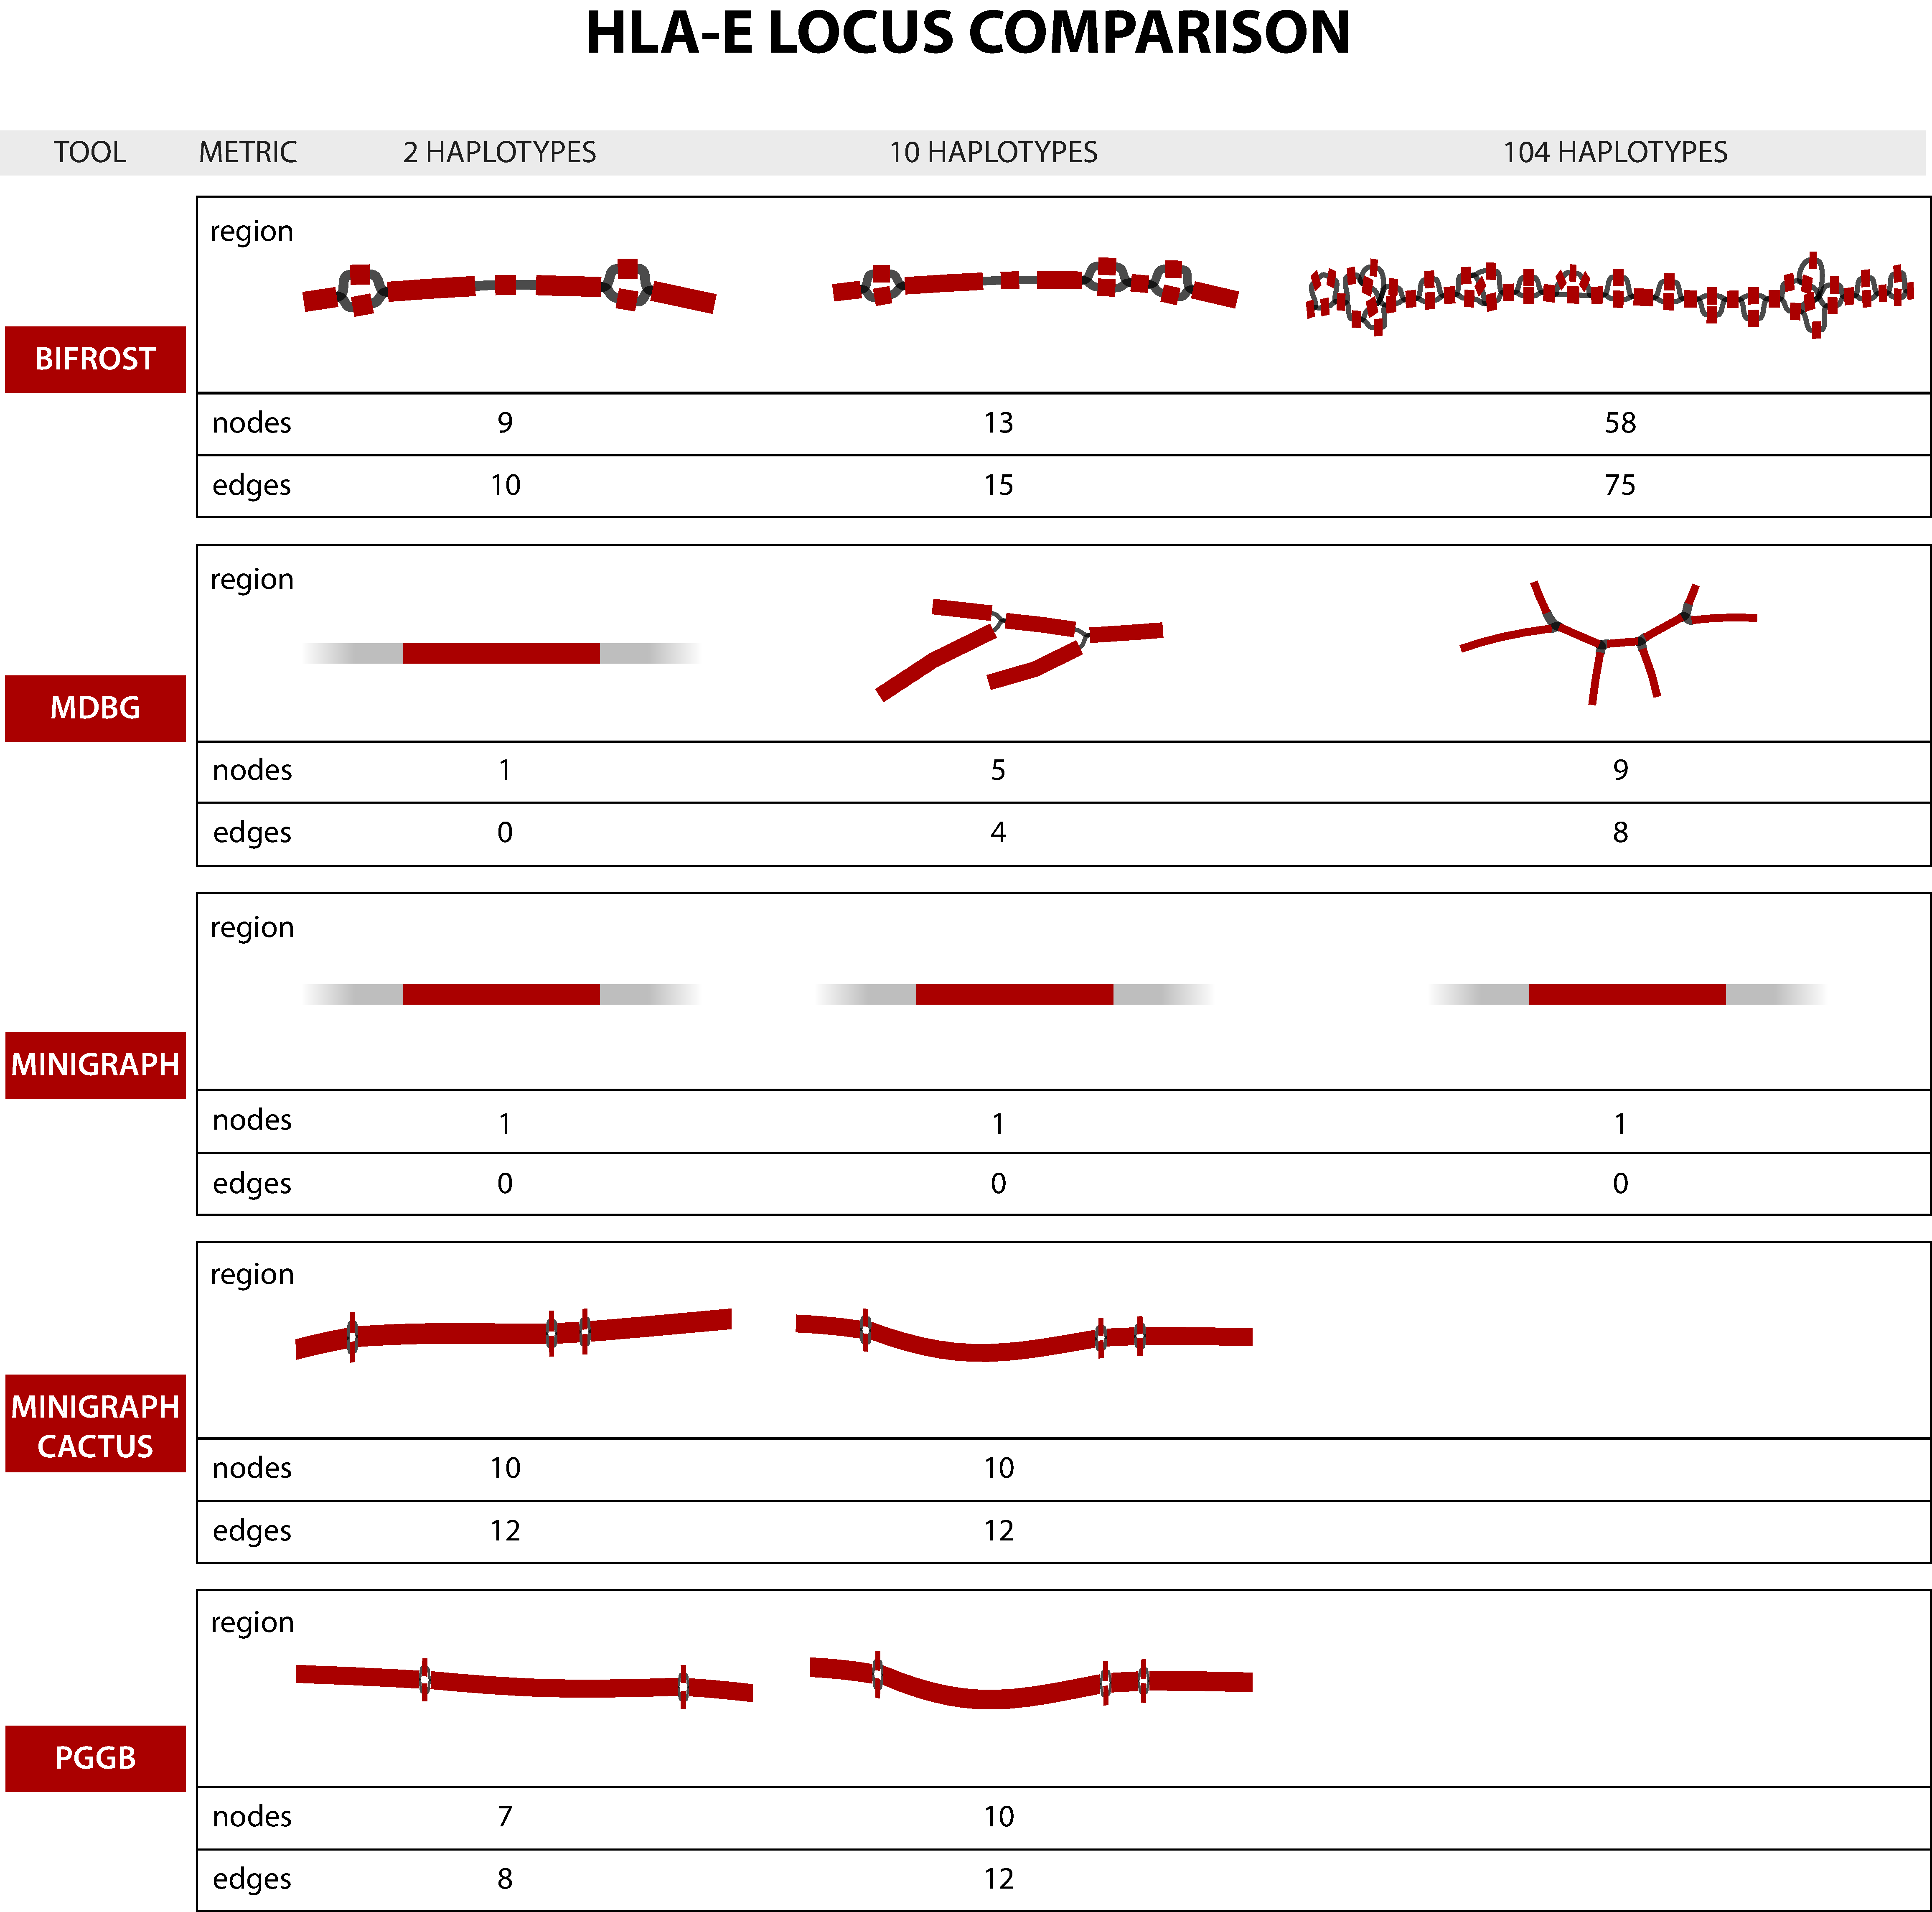
\includegraphics[width=0.95\textwidth]{figures/paperI/hla-e_corrected.pdf}
    \caption{Representations of the HLA-E locus by five graph construction methods over three increasing large human pangenomes. Nodes highlighted in red contain part of the locus sequence. The numbers of nodes and edges displayed below each graph concerns the whole subgraph (both red and grey nodes). %, i.e. nodes and edges directly or indirectly attributed to the sequences that represent the locus. 
    \minigraph, on H2, H10 and H104, and \mdbg, on H2, have only a portion of one node highlighted since the 4.8k bp region is contained inside a single, long node.} 
    \label{fig:HLA-E}
\end{figure}

\paragraph{\textbf{\textup{HLA complex locus: high complexity region}}}

Figure \ref{fig:HLA-A} is the counterpart of Figure~\ref{fig:HLA-E} for the complex locus part. In this case the overall interpretability of the region is more challenging, as the number and the structure of the variations is different than in HLA-E. It is also more difficult to compare across tools. Base-level variations, e.g. SNPs, are not visually recognizable in Figure~\ref{fig:HLA-A} in the methods that retain them (i.e. \pggb, \mcactus and \bifrost) due to the large sizes of graphs.

There are notable differences in how  tools represent the variation, which is well-illustrated in the H2 dataset. While \minigraph renders H2 as a single sequence plus a large structural variant (SV) of $\approx$ 52k bp, \pggb separates it into two paths that differ by $\approx$ 54k bp in length. \bifrost represents a detailed bubble that contains many variations inside each path. In \mdbg, even extracting the complete locus is a challenge as many of the subgraph nodes were not selected by our procedure. \mcactus adds base level divergences between haplotypes on top of \minigraph SV graph.

These differences between representations are further accentuated in the H10 dataset. For it, \pggb tends to separate the haplotypes into different paths, \bifrost renders consistently the same compacted representation and \minigraph neglects most of the small differences but is able to display accurately the general picture, and \mcactus, as in H2, adds small variations on top of \minigraph structure. 


\begin{figure}[htp]
    \centering
    \includegraphics[width=0.95\textwidth]{figures/paperI/hla-a_corrected.pdf}
    \caption{Representations of the complex HLA region by five graph construction methods over three increasing large human pangenomes. 
 See caption of Fig.~\ref{fig:HLA-E} for details. 
 %.Nodes highlighted in red are the ones that contain part of the locus sequence. The number of nodes and edges displayed represent the ones directly or indirectly attributed to the sequences that represent the locus.
    }
    \label{fig:HLA-A}
\end{figure}

\subsection*{\textbf{Uncovering characteristics of graphical pangenome tools}}
\label{sec:uncovering}
The data structures generated by pangenome building tools are expected to facilitate comparisons between the input genomes. In addition pangenome graphs should be stored in such a way to be easily used by downstream applications.
We identify 8 important features for pangenome graph construction tools: i) stability, ii) editability, iii) accessibility by downstream applications, iv) haplotype compression performance v) ease of visualization, vi) quality of metadata and annotation. Two other but important features, scalability and interpretability of produced graphs, were already discussed in Sections "Scalability and characteristics of pangenome graph construction tools" and "Interpretation of variation in pangenome graphs: focus on two HLA loci". %\ref{sec:scalablility} and \ref{sec:loci}. 
Table \ref{tab:tools_consideration} summarizes some of the following considerations on the relative strength of the tools.

\paragraph{\textbf{\textup{Editability and dynamic updates}}}
%\noindent\textbf{EDITABILITY AND DYNAMIC UPDATES} 
As more high quality assemblies will be generated in the near future, haplotypes may be added to a pangenome, or replaced by improved versions. Updating an existing data structure instead of rebuilding it from scratch is both computationally and energetically efficient. 
However, many succinct data structures currently used in pangenome representation are static, i.e. cannot be updated. %Current
Some methods allow a restricted set of editing operations.
\minigraph allows to add new haplotypes on top of an already built graph. \bifrost provides C++ APIs to add or remove \mbox{(sub-)sequences}, \kmers and colors from the ccdBG.
\pggb, using \odgi~\cite{odgi}, allows specific operations that delete and modify nodes and edges and add and modify paths through the graph. As \mcactus can be opened with \odgi, it supports the same operations as \pggb. 
The current \mdbg implementation uses a dynamic hash table, but does not expose an interface that supports updates.

\paragraph{\textbf{\textup{Stability}}}
%\noindent\textbf{STABILITY} 
Counter-intuitively, a pangenome graph construction tool may in some cases generate different outputs when executed multiple times with the same haplotypes as input. This \emph{unstability} could be due to a permutation in the order of the sequences given as input, or non-determinism in the construction algorithm.
Yet in order to facilitate the reproducibility of results, pangenome building tools should generate an unchanged output from the same set of input sequences, independently of the particular run or the order in which these are given.
We performed two tests to evaluate tool stability: i) we run the tools 3 times using as input the same H10 dataset and ii) we run the tools twice on shuffled input sequences, i.e. changing the order of the haplotypes of H10. 

\bifrost and \mdbg constructed exactly the same pangenome on every test, as by definition, de Bruijn graphs are stable.
\minigraph generates identical graphs on identical inputs, but generates slightly different graphs when the input is permuted. Indeed the construction algorithm of \minigraph is order-sensitive as it augments the existing graph structure by aligning the next given haplotype to it and adding divergent sequences. 
\mcactus generates slightly different graphs on identical input. 
\pggb\ generated slightly different graphs while maintaining the same haplotype sequences in the paths. The overall representation of the input genomes is therefore preserved, while the topology of the variation graph varies. The first two of the three phases of the \pggb pipeline (all-vs-all alignment and graph imputation) produce the same result on different runs with the same input but differences arise when the order of the input haplotypes changes. Most of the differences in the graph topology are thus due to the final smoothing steps.

\paragraph{\textbf{\textup{Accessibility by downstream applications}}}
% \noindent\textbf{ACCESSIBILITY BY DOWNSTREAM APPLICATION} 
\label{subs:downstream}
To facililate their adoption, pangenome representations should be easily processed by downstream analyses. 
De Bruijn graphs are challenging to analyze due to their high number of nodes, edges, and redundancy (the $k-1$-overlaps between nodes).
Though De Bruijn graph representations usually support queries of presence/absence on nodes (as in \bifrost), they lack tools able to perform more elaborate analyses such as those discussed in Section "Interpretation of variation in pangenome graphs: focus on two HLA loci", e.g. incorporating haplotype information at the \kmer level. 
On the other hand, variations graphs with paths provide more flexibility, i.e. as in \pggb and \mcactus with the \odgi visualization toolkit.
Finally in \minigraph, which considers a narrower spectrum of variants, the absence of path information prevents haplotype-level analysis; haplotypes would need to be manually mapped back to the graph. 
The choice of the pangenome building tool depends on the envisioned application. \mbox{\pggb} and \mbox{\mcactus} graphs have been shown to outperform linear references for short read mapping, genotyping and RNA sequencing mapping \mbox{\cite{hdpr}}. As these two methods  are complex pipelines based on multiple tools where parameters have been carefully set, they can be more challenging to install and run than single integrated tools. \mbox{\minigraph} alone can also be used if the focus is on structural variation instead of SNPs or small indels, and to quickly produce a pangenome graph for complex loci visualization and interpretation. The dBG-based approaches show that, for example with \mbox{\bifrost}, they retain the same base-level information as more computational-heavy variation graph approaches, but the lack of tools to use them for analysis limits their adoption.

\paragraph{\textbf{\textup{Haplotype compression}}}
%\noindent\textbf{HAPLOTYPE COMPRESSION} 
Building a graph pangenome can be seen also as a way to store, compact and retrieve the input haplotypes. As the number of new assemblies is growing faster than the data storing capacity, pangenomes can potentially help save storage space. This is highlighted by the disk space reported in Table~\ref{tab:computational_metrics}, which is consistently smaller than the sum of haplotype sizes for all methods and datasets.

In order to losslessly retrieve the input genomes from a pangenome, the  representation has to store all variations from the original haplotype sequences as paths in the graph. \pggb and \mcactus fall into this category while the other three considered tools do not store paths, or do not consider all variations, thus they are lossy.

Of note, the GBZ tool~\cite{gbz} enables graph pangenomes that store paths in the GFA file format %(the consensus file format used) 
to be stored in a lossless compressed form. It uses a Graph Burrows-Wheeler transformation to compress the graph in a more efficient way than using gzip~\cite{gbz}. Using GBZ, the pangenomes generated by \pggb and \mcactus are losslessly compressed with space gains of 3.5-5x.


\paragraph{\textbf{\textup{Ease of Visualization}}}
%\noindent\textbf{EASE OF VISUALIZATION} 
Visualizing large graphs which exceed hundreds of thousands of node is a challenge that exceeds the scope of pangenomics. The H104 pangenomes  are difficult to visualize.
Among the visualization tools considered by the Human Pangenome Reference consortium~\cite{hpp}, 
only \bandage is able to display the \minigraph or \mdbg H104 graphs, which contains a few million nodes. We reduced the number of nodes and edges of \pggb, \mcactus and \bifrost H10 graphs by collapsing isolated subgraphs representing SNPs or indels up to 10k bp (using the command \texttt{gfatools asm -b 10000 -u}). % to be able to display them. 
%Generally, general-purpose graph drawing tools able to visualize graphs with millions of nodes are needed, in particular to extract and display specific loci.

\paragraph{\textbf{\textup{Quality of Metadata and Annotation}}}
%\noindent\textbf{QUALITY OF METADATA AND ANNOTATION} 
Augmenting pangenome structures with information from other omics data would increase pangenome relevance in biological discoveries. As biobanks are rapidly growing, more data is available on regulatory regions, transcriptomics, CNVs and other medically relevant traits~\cite{100000genomes,ucla}. Pangenome data structures could leverage such information, and some of the considered tools offer basic functionality in this sense.
\bifrost provides a function to link data to graph vertices through C++ APIs. \pggb and \mcactus, using \odgi, offer annotation capabilities through insertion of paths or BED records. \minigraph and \mdbg do not offer any annotation feature. 
Specifically, in order to enhance a pangenome graph with metadata (for example with genes and regulatory regions known variants), it is desirable to maintain compatibility with methods and data formats that use a linear reference. One could conceivably project data from a graph to a reference genome to continue downstream analyses using linear coordinates. A simple method to achieve this compatibility, in our view, is to store the reference genome of interest inside the graph pangenome that supports retrieving such a reference. Variation graphs built using \mbox{\pggb or \mcactus}, due to their locally acyclical and directed construction and their use of haplotype paths, store all the coordinates needed for such a task. Haplotype paths play an important role as they avoid additional mapping to the graph, by using the \mbox{\odgi}tool to extract or inject the required information. \mbox{\minigraph} does not store haplotype paths and requires mapping sequences to the graph to restore haplotype information. On the other hand, De Bruijn graphs, using associated color data, can record the membership of k-mers to a reference sequence, yet one cannot fully reconstruct a haplotype unless k-mers positions are also stored.
\begin{table}
\centering
 \caption{\textbf{Relative strengths of five pangenome graph construction tools}\\
 Explanation of rows:
 1) efficacy of construction algorithm, measuring wall-clock time;
 2) degree to which variants (e.g. SNPs) are retained;
 3) ability of a tool to perform well on large datasets, both in comparison to other tools but also compared to smaller datasets;
 4) ability to modify the produced data structure to add or remove haplotypes; 
 5) property of producing the same result irrespective of perturbations, such as permutation of the input order, and repeating the same run;
 6) existence of tools (and operations) that can be applied to the resulting graphs; 
 7) whether input haplotypes information is retained by the tools, and if so, its space efficiency;
 8) whether the entire graph can be directly visualized and interpreted; 
 9) easiness of 'zooming in' a specific genomic region and interpret variants;
 10) summarizes the functionalities provided by the tools to annotate the pangenomes with genomic data;
 11) ability to share information between the graph and a linear reference.
}
\resizebox{\textwidth}{!}{
\begin{tabular}{|l c c c c c|} 
 \hline
 Metric & \bifrost & \pggb & \mcactus & \minigraph & \mdbg\\
 \hline
  1) Construction speed & $\bullet\bullet\circ$ & $\bullet\circ\circ$ & $\bullet\circ\circ$ &  $\bullet\bullet\circ$ & $\bullet\bullet\bullet$\\
 \hline
 2)  Variations & $\bullet\bullet\bullet$ & $\bullet\bullet\bullet$ & $\bullet\bullet\bullet$ & $\bullet\bullet\circ$ & $\bullet\bullet\circ$\\
 \hline
  3) Scalablilty & $\bullet\bullet\bullet$ & $\bullet\circ\circ$ & $\bullet\circ\circ$ & $\bullet\bullet\circ$ & $\bullet\bullet\bullet$\\
 \hline
  4) Editability & $\bullet\bullet\bullet$ & $\bullet\bullet\circ$ & $\bullet\circ\circ$ & $\bullet\bullet\circ$ & $\bullet\circ\circ$\\
 \hline
 5) Stability & $\bullet\bullet\bullet$ & $\bullet\circ\circ$ & $\bullet\circ\circ$ & $\bullet\bullet\circ$ & $\bullet\bullet\bullet$\\
 \hline
 6) Accessibility by downstream applications & $\bullet\circ\circ$ & $\bullet\bullet\bullet$ & $\bullet\bullet\bullet$ & $\bullet\bullet\circ$ & $\bullet\circ\circ$\\
\hline
 7) Haplotype compression performance & $\bullet\bullet\circ$ & $\bullet\bullet\bullet$ & $\bullet\bullet\bullet$ & $\bullet\circ\circ$ & $\bullet\circ\circ$\\
 \hline
8) Ease of visualization  & $\bullet\circ\circ$ & $\bullet\bullet\circ$ & $\bullet\bullet\circ$ & $\bullet\bullet\bullet$ & $\bullet\bullet\bullet$ \\
 \hline
 9) Loci visualization and interpretability   & $\bullet\circ\circ$ & $\bullet\bullet\circ$& $\bullet\bullet\bullet$ & $\bullet\bullet\circ$  & $\bullet\circ\circ$\\
 \hline
  10) Metadata and annotation   & $\bullet\bullet\circ$ & $\bullet\bullet\bullet$ & $\bullet\bullet\circ$ & $\bullet\circ\circ$  & $\bullet\circ\circ$\\
 \hline
11) Compatibility with a linear reference coordinates & $\bullet\circ\circ$ & $\bullet\bullet\bullet$ & $\bullet\bullet\bullet$ & $\bullet\bullet\circ$  & $\bullet\circ\circ$\\
 \hline
\end{tabular}}
    \label{tab:tools_consideration}
\end{table}

\section{Discussion}
Five state-of-the-art pangenome graphs construction tools were compared on the representation of up to 104 human haplotypes. The approaches significantly differ in terms of speed, graph size, and representation of variations. We find that it remains computationally prohibitive to generate human pangenome graphs for hundreds of haplotypes, especially while retaining all variations. Each approach has its own set of strengths, and ultimately the choice of the method depends on the downstream application. In addition, several takeaway points emerged from our analysis.

First, our focused analysis of HLA loci revealed that de Bruijn graphs and variation graphs represent genomic variations equally well as pangenomes.  This is of particular importance as also shown by the draft human pangenome references~\mbox{\cite{hdpr}}: pangenomes are pivotal to trace complex and clinically relevant loci. While de Bruijn graphs are faster to construct, more stable, and scale better in terms of input size, the resulting graphs are challenging to interpret downstream. Variations graphs on the other hand are more practical to analyze at the expense of a less efficient construction step. Their visualization are more straightforward to interpret, mostly due to not having cycles, and provide insights into loci differences. 

Second, we can highlight two categories of pangenomic methods that have distinct application domains. \pggb, \mcactus and \bifrost store all possible variations, and keep haplotype information as paths or colors. They provide a complete picture of the set of variations in the input genomes which makes them difficult to analyze. They can be used for a large variety of genomic analysis, as shown for \mbox{\pggb} and \mbox{\mcactus}~\mbox{\cite{hdpr}}. \minigraph and \mdbg generate 'sketched' pangenome graphs that consider only large variants, ignoring smaller differences, and are more efficient to construct and visualize. They can be used for large scale characterization of variation in population, as proven for bacteria \mbox{\cite{mdbg}}.

Third, every tool possesses an exclusive set of features.
\pggb facilitates downstream analyses using the companion tool \odgi. It allows to precisely extract and browse any locus of interest. It is the only tool that generates variation graphs without a reference. It also keeps a lossless representation of the input sequences.
\minigraph generates a pangenome graph based on a reference sequence taken as a backbone. Its shines in the representation of complex structural variations, but does not include small or inter-chromosomal variations.
The pipeline \mcactus, that uses the \cactus base aligner, can be used to add small level variations on top of the \minigraph graph and to keep a lossless representation of the input sequences.
\bifrost illustrates that classical de Bruijn graphs are scalable, stable, dynamic, and store all variations. However, extracting information from them remain a challenge.
Lastly, \mdbg\ is the fastest construction method which generates an approximate representation of differences between haplotypes. As discussed in Section "Accessibility by downstream applications", these features enable different genomic analyses and downstream applications.

\section{Conclusions}
In conclusion, our results highligh the strengths and weaknesses of current pagnenome construction tools for human applications, with specific focus on how do they represent specific loci of medical relevance. We also provide insights on the features they possess and point out their best application domains.
In our view, future directions for human pangenomes building tools should focus on tackling efficiency bottlenecks, aiming to represent hundreds to thousands of haplotypes. Representations should further be lossless and represent the input haplotypes as paths in the graph. 
Such features would unlock many other applications such as lossless compression of haplotypes and cancer copy number variant analysis. 
Finally, we recognize the need for more user-friendly tools that can be used by biologists and that can translate complicated questions into  graph queries. While \odgi begins to address these questions in variation graphs, other approaches have not yet provided user-friendly interfaces. A package similar to \odgi for de Bruijn graphs would help fully realize their potential.

\section{Methods}
\subsection*{\textbf{Datasets and haplotypes collection}}
\label{sec:datasets}
In order to evaluate the state of current human pangenome representations, we sought to build a human pangenome that contains all publicly available high-quality human haplotypes. We collected from two different sources 102 different haplotypes from the genome of 51 individuals, and also used the two reference genomes, GRCh38 from the Genome Reference Consortium (GRC) \cite{grc} and CHM13 v2.0 cell line of the T2T Consortium~\cite{t2t}.
Five haplotypes correspond to Google Brain Genomics DeepConsensus \cite{deepconsensus} assembly dataset: they are hifiasm assemblies of PacBio Hi-Fi reads corrected with DeepConsensus. The average of their N50 is 37,99 Mbp. 
The remaining haplotype assemblies as well as the T2T reference are from the Human Pangenome Reference Consortium (HPRC) year-1 freeze~\cite{hpp}, and GRCh38 is from the GRC. Their average N50 is 40.3 Mbp. Since HG002 is contained in the DeepConsensus data, the HPRC HG002 haplotypes were not used.
The origin and the sex of the individuals are diverse %to aim for a 
and provide a fair representation of the diversity in human population: out of 51 total individuals, 21 are males and 30 are females and they represent 14 different ethnic groups, from US to Africa and Asia. We did not perform any additional selection, regarding sex and ethnicity, on these public datasets as our main goal was to use as many genomes as possible. However, the HPRC stated that the genomes were selected to represent genetic diversity in humans~\mbox{\cite{hdpr}}.

To evaluate the scalability of pangenome construction tools, we created three datasets of increasing size: 1) 2 haplotypes from the same individual, HG006, 2) 10 haplotypes from 5 different individuals (HG002, HG003, HG004, HG006 and HG00735) and finally 3) all of the 104 haplotypes. To test whether the order of the input sequences matters, we considered various random orderings for the 10 haplotypes in Dataset 2. Since \minigraph needs a reference sequence as fist haplotype in order to correctly build the graph, we generated specific 2 and 10 haplotypes datasets with the first haplotype replaced by the reference genome CHM13. This was applied to the \mcactus pipeline as well as it uses \minigraph variation graphs.

 \begin{table}
  \centering
  \setlength{\tabcolsep}{5pt} 
  \caption {\textbf{Description of the three datasets generated to test the scalability of the tools}
 \\
 Data sources: 
   $^1$ Google Brain Genomics~\cite{google-assemblies}; $^2$ Human Pangenome Reference Consortium~\cite{HPRC-haplotypes}; $^3$ 1000 Genomes Project~\cite{HPRC-haplotypes}; $^4$ Telomere to Telomere Consortium~\cite{HPRC-haplotypes}.
   \label{tab:datasets}}
  \renewcommand{\arraystretch}{1.2}
\begin{tabular}{|c c c|}
  \hline
  \centering
   Haplotypes & Project & Bases \\
   \hline
    2 & Google$^1$ & 5.9 Gbp\\
   10 & Google, HPRC$^2$ & 30 Gbp \\
    104 & Google, HPRC, 1KG$^3$, T2T$^4$ & 313.6 Gbp \\
    \hline
  \end{tabular}
\end{table}
 
\subsection*{\textbf{Pangenome graph construction tools}}
\label{sec:tools}

We evaluated tools that generate graph pangenomes as variation graphs and colored compacted de Bruijn graphs. Variation graphs are generally locally acyclic while de Bruijn graphs have cycles. In variation graphs, nodes represent sequences and edges represent immediate sequence adjacency without overlap. Variation graphs are generally easier to visualize and to interpret while challenging to construct at scale and, apart from \pggb, require a reference genome. In de Bruijn graphs (\dbg), nodes are \kmers (string of length k) and edges are (k-1)-overlaps between nodes. In practice, \dbgs are represented in a compact way where all nodes along unbranching paths are compacted into \emph{unitigs}. The resulting graph is called compacted De Bruijn Graph, where nodes are unitigs and edges represent (k-1)-overlaps. 
As shown in Figure \ref{fig:figure1}, de Bruijn graphs %are easier to construct and are more standardized but 
result in large graphs that pose visualization and interpretation challenges, in particular as there is no alignment to a reference.

\begin{itemize}
\item
\bifrost constructs dynamic, coloured compacted de Bruijn Graphs (\emph{\ccdbg}). It first generates a standard \dbg using an efficient variant of Bloom Filters and then computes the compacted \dbg from it.
Colors, i.e. identifiers representing the sample origin of each k-mer are added by storing an array per \kmer. A human genome \ccdbg typically consists of a single large connected component, as common \kmers are shared between chromosomes. This pangenome representation contains all the variations present in input sequences.

\item
\mdbg builds a variant of de Bruijn graphs called a minimizer-space de Bruijn Graph (\mdbg), which is efficient to construct as it only considers a small fraction of the input nucleotides. Color information is currently not supported in the implementation. Similarly to Bifrost, a \mdbg also typically represents a human genome as a single large connected component, albeit with orders of magnitude less nodes. Minimizer-space de Bruijn graphs mostly discard small variants, yet are sensitive to heterozygosity which creates branches in the graph.

\item
\minigraph constructs a directed, bidirected and acyclic variation graph iteratively by mapping new haplotypes using a combination of the minimap2 tool and the graph wavefront alignment algorithm. The first input sequence acts as a  backbone for the whole representation.
The sample(s) of each node are stored in a rGFA output file.
\minigraph considers only variations longer than 50 bps hence it is oblivious to isolated SNPs and small indels: even if it produces base-level alignment for contigs, the graphs are not a base-level resolution. The resulting graph is divided into connected components that correspond to the chromosomes present in the first given input genome.
%, yet can represent large divergent regions at base-pair resolution
\item
\mcactus is a variation graph construction pipeline that combines \minigraph to generate a structural variations graph and \cactus base aligner to generate base-level pangenome graphs of a set of input assemblies and embg: The definition of \label has changed! Check your packages! Replacing it with the kernel definition on input line 145.ed haplotypes paths. \cactus~\cite{cactus} is a highly accurate and scalable reference-free multiple whole-genome alignment tool, that in this pipeline considers the reference sequence used by \minigraph to ensure that the resulting variation graph is acyclic. The final graph is further normalized using GFAffix\cite{gfaffix}. The pipeline allows to generate multiple graphs, one for each chromosome, or produce a single graph that includes inter-chromosomal variants.

\item
\pggb is a directed acyclic variation graph construction pipeline rather than a single tool. It calls three different tools: pairwise base-level alignment  of haplotypes using wfmash \cite{wfmash}, graph construction from the alignments with seqwish \cite{seqwish}, graph sorting and normalization with smoothxg and GFAffix \cite{smoothxg,gfaffix}.
The resulting variation graph represents variations of all lengths present in the input sequences.
\end{itemize}


\begin{table}
\centering
\caption{ \textbf{URL, version, pangenome representation and parameters of the three analyzed tools.}\\ pggb/0.2.0 used wfmash v0.7.0, seqwish v0.7.3 and smoothxg v0.6.1.}
\resizebox{\textwidth}{!}{
\begin{tabular}{|c c c c c|} 
 \hline
Tool  &  Github repository & Graph type & Version & Parameters \\ 
 \hline \hline
\bifrost & pmelsted/Bifrost  & De Bruijn graph  & 1.0.5 & -k100 -c \\ 
 \hline
\pggb &   pangenome/pggb & variation graph  & 0.2.0 & -p 98 -s 10000 -k 311 -G 13033,13117\\ &&&& -O 0.03 -v -t 8 -T 8 -A -Z \\ 
\hline
 \minigraph & lh3/Minigraph  & variation graph &   0.18 & -cxggs\\ 
 \hline
  \mcactus & ComparativeGenomics  & variation graph &   2.2.3 & --maxLen 10000 --delFilter 10000000 \\ & Toolkit/cactus &&&\\ 
 \hline
 \mdbg  & ekimb/rust-mdbg  & De Bruijn graph &  1.0.1 & -k 10 -d 0.0001 --minabund 1 --reference\\ 
 \hline
\end{tabular}}
    \label{tab:url}
\end{table}



\section*{Supplementary Information}

\subsection*{\textbf{Benchmark infrastructure}}

Running time of pangenome construction tools was measured as wall clock time and peak memory as maximum resident set size using the \texttt{time} command. Other metrics were obtained with custom Python scripts. All benchmarks were performed on a Supermicro Superserver SYS-2049U-TR4, with 3 TB RAM and 4 Intel SKL 6132 14-cores @ 2.6 GHz, using 8 cores. \\

\subsection*{\textbf{TwoPaCo}}
\label{app:twopaco}
We did not consider \twopaco as it is redundant with \bifrost. Both methods construct the same de Bruijn graphs.
\twopaco is a method for constructing \ccdbgs by finding junction \kmers at the boundaries of unitigs or in branching nodes. It consists of two main steps in which it approximates the dBG with a Bloom filter in order to reduce the size of the problem and then runs a two pass highly parallel algorithm on it. It constructs ccdBGs similarly to \bifrost. \bifrost  is faster, supports edit operations, and accepts also reads other than assemblies as input. We tested both tools on NCBI datasets from three different known human variation regions part of the human leukocyte antigen (HLA) complex: HLA-A, MICB and TAP1. These loci have different number of sequences and have complexity and length. The resulting graphs have exactly the same k-mer content and substantially equal topology. The difference is that \twopaco considers sequences with IUPAC 'N' bases while \bifrost does not and that in some cases \twopaco renders some unitigs split in two or more consecutive nodes.

\subsection*{\textbf{Loci extraction method}}
\label{app:extraction}
For \bifrost and \mdbg graphs, nodes corresponding to the input sequences are identified with \graphaligner\cite{graphaligner} and the subgraph is extracted using the \bandage \emph{reduce} function. As the aligned nodes are not expected to represent the full diversity of the population in the pangenomes, the considered portion of the graph contains also nodes up to a certain distance from the aligned ones: 1 for \mdbg and 3 for \bifrost. This number is based on the size of the sequences spelled by the nodes and on the considered variations. Artifacts, mostly tips, that are not part of the locus of interest are removed with a custom python script. For \minigraph generated graphs, the \minigraph own alignment function has been used to identify the nodes and then \bandage is used to extract the subgraph. For \pggb, first we generate a bed file of the position of the region of interest in every haplotype used to construct the graph. The ranges are derived from aligning them to the locus sequence(s) using minimap2 \cite{minimap2}. The graph corresponding to the region is then extracted using the \odgi extract and \odgi view functions. For \mcactus we use the same strategy as \pggb, with the difference that the bed file is only for the reference CHM13, present in the graph. \\
The annotation of the specific loci in the subgraph is done using nodes from the alignment with \minigraph or \graphaligner to the subgraph. This makes it possible to highlight multiple sections in the region, as, for example, genes and pseudogenes of interest. 

\section*{\textbf{Availability of data and materials}} %Reproducibility and Data Availability
The scripts used to generate and analyse the pangenomes can be found at \cite{source-code-github}\cite{source-code-zenodo} under MIT license.
Google Brain Genomic assemblies can be found at \cite{google-assemblies}. \\
HPRC assemblies, CHM13 and GRCh38 can be found at \cite{HPRC-haplotypes}.

\section*{\textbf{Funding}}
R.C was supported by ANR Full-RNA, SeqDigger, Inception and PRAIRIE grants (ANR-22-CE45-0007, ANR-19-CE45-0008, PIA/ANR16-CONV-0005, ANR-19-P3IA-0001). This project has received funding from the European Union’s Horizon 2020 research and innovation programme under the Marie Skłodowska-Curie grants agreements No. 872539 and 956229.

\section*{\textbf{Author's contributions}}
FA, YD and RC conceived and designed the project. FA implemented the scripts. FA and PL ran the experiments. FA, YD, PL and RC wrote the paper. The authors read and approved the final manuscript.

%% Format bibliography like a section, not a chapter:
% \printbibliography[heading = subbibliography]
% \stopcontents[chapters]© Francesco Andreace, 2024

Series of dissertations submitted to the
Insitut Pasteur Paris, Universite’ de Paris Cite, University of Oslo
No. 1234
ISSN 1234-5678
All rights reserved. No part of this publication may be
reproduced or transmitted, in any form or by any means, without permission

\paragraph{Authors' affiliations}
\begin{description}
    \item[Francesco Andreace]
    Institut Pasteur, Université Paris Cité, G5 Sequence Bioinformatics \\
    Sorbonne Université, Collège doctoral \\
    25-28 Rue du Dr Roux, 75015 Paris


    \item[Pierre Lechat]
    Bioinformatics and Biostatistics Hub, Institut Pasteur, Université de Paris Cité \\
    25-28 Rue du Dr Roux, 75015 Paris

    \item[Yoann Dufresne]
    Institut Pasteur, Université Paris Cité, G5 Sequence Bioinformatics \\
    Bioinformatics and Biostatistics Hub, Institut Pasteur, Université de Paris Cité \\
    25-28 Rue du Dr Roux, 75015 Paris

    \item[Rayan Chikhi]
    Institut Pasteur, Université Paris Cité, G5 Sequence Bioinformatics \\
    25-28 Rue du Dr Roux, 75015 Paris
\end{description}

\section{Perspectives}

\begin{itemize}
    \item In perspective the work of this article could have been extended to provide a pipeline (on nextflow for example) to benchmark all pangnomes constructed independently of the data structure used to provide the features described on the paper. This would have provided a platform to independently benchmark new pangenomes and rendered the paper not only useful as review and hints for end-users but also as benchmarking for new methods or methods improvement;
    \item Among the features I could have included it would have been useful: \begin{enumerate}
        \item count SNPs (trivial for VGs, not trivial for DBGs);
        \item node length distribution;
        \item node degree distribution;
        \item conversion of variation graphs to De Bruijn graphs (extendin nodes smaller than k) to validate if they contain the same information/ did not loose information - see \minigraph example;
    \end{enumerate}
\end{itemize}
    %\author
{
    Francesco Andreace
    \and
    Pierre Lechat
    \and
    Yoann Dufresne
    \and
    Rayan Chikhi
}
\title{Comparing methods for constructing and representing human pangenome graphs}
\metadata
{
    Published in \emph{Genome Biology},
    November~2023,
    volume~24,
    issue~1,
    article number 274.
    \doi{10.1186/s13059-023-03098-2}.
}
\maketitle
\label{pap:gb_pdf}

\section{Motivation}
This paper originates from an early discussion, after completing a torough review of the state-of-the-art of computational pangenomics. What tool should be used if we would like to build a human pangenome for a large cohort of eukaryotes, for example humans. The answer is more complex than a list of widely used tools. There are multiple ways of representing a group of genomes to be analyzed or used jointly. One that took traction in the last few years has been graphs. Graphs can represent the sequence information as labels of nodes and the difference between the genomes as different paths in the graph. Depending on the particular representation, edges can represent adjacencies, i.e the genome is spelled by a walk on nodes connected by an edge, or overlaps , i.e. the suffix of a node is the prefix of the next node connected by the graph. In this article, we surveyed the the methods and tools that build such graphs, then tested them on different datasets and finally analyzed their features. The result is a small guide on which are the best applications for each of these tools and which are the weaknesses they suffer from.


\includearticle{sections/pangenome_paper}

\section{Perspectives}
The work of this article has adressed several key issues in both 
\begin{itemize}
    \item how to evaluate if a pangenome graph construction method is generating a data structure that faithfully represent the underlying genetic information and variations;
    \item In which areas in each methodology that should focus in order to produce for the community a useful tool.
\end{itemize}    
On this realization, this work could be relatively easily extended to provide a pipeline (on Nextflow, for example) to benchmark all pangnomes constructed independently of the data structure used to provide the features described on the paper. This would provide a useful platform to independently benchmark new pangenomes and rendered the paper not only useful as review and hints for end-users but also as benchmarking for new methods or methods improvement.
Moreover, other useful features could be added, among which
\begin{enumerate}
    \item count SNPs (trivial for VGs, not trivial for DBGs);
    \item node length distribution;
    \item node degree distribution;
    \item conversion of variation graphs to De Bruijn graphs (extending nodes smaller than k) to validate if they contain the same information and did not loose some (this behaviour is expected by \minigraph, or \mcactus, for example).
\end{enumerate}
Finally, the paper has been well received by the community, mostly because more methods in pangenomics are being published and a critical survey of which representation is better   

    %\author
{
    Victor Levallois
    \and
    Francesco Andreace
    \and
    Bertrand Le Gal
    \and
    Yoann Dufresne
    \and
    Pierre Peterlongo
}
\title{The Backpack Quotient Filter: a dynamic and space-efficient data structure for querying $k$-mers with abundance}

\metadata
{   
    Presented at \emph{RecombSeq}
    April-2024,
    \doi{10.1101/2024.02.15.580441}.
    % Published in \emph{Genome Biology},
    % volume~24,
    % issue~1,
    % article number 274.
}
\maketitle
\label{pap:second}

\section{Motivation}
This work stems from the very need of storing very large sequencing information from complex biological samples (like metgenomes) with the goal of being able to access it in a fast and randomized way. Complex biological datasets
\begin{abstract}
Genomic data sequencing has become indispensable for elucidating the complexities of biological systems. As databases storing genomic information, such as the European Nucleotide Archive, continue to grow exponentially, efficient solutions for data manipulation are imperative. One fundamental operation that remains challenging is querying these databases to determine the presence or absence of specific sequences and their abundance within datasets.

This paper introduces a novel data structure indexing $k$-mers (substrings of length $k$), the Backpack Quotient Filter (BQF), which serves as an alternative to the Counting Quotient Filter (CQF). The BQF offers enhanced space efficiency compared to the CQF while retaining key properties, including abundance information and dynamicity, with a negligible false positive rate, below $10^{-5}\%$. The approach involves a redefinition of how abundance information is handled within the structure, alongside with an independent strategy for space efficiency. 

We show that the BQF uses 4x less space than the CQF on some of the most complex data to index: sea-water metagenomics sequences. Furthermore, we show that space efficiency increases as the amount of data to be indexed increases, which is in line with the original objective of scaling to ever-larger datasets.
    
    \textbf{Availability:} \url{https://github.com/vicLeva/bqf} 
\end{abstract}

\footnotetext
{%
    University of Oslo,
    Postboks 1337 Blindern, 0316 Oslo, Norway,
    \href{mailto:fauthor@uio.no}{fauthor@uio.no}
}

\section{Introduction}

Genomic data sequencing is a powerful tool for understanding the intricacies of biological systems. Sequencing produces plain text, organized as reads in files. Most of these files are gathered in public databases like the European Nucleotidic Archive (ENA)~\cite{burgin2023european} that weighs 54.5PB by early 2024. The size of the databases follows exponential growth, and thus we need appropriate solutions to manipulate the data it contains. One simple operation that we are not yet able to achieve (in reasonable time and resources) is to query the database and then, for each dataset, answer if a sequence is present or absent. Even better, answer for each dataset how many times a sequence is present: its abundance. To this end, we use indexing data structures that can handle another representation of the data, making it easier to query afterward. Some of the current indexing data structures use sets of $k$-mers (substrings of length $k$, $k$ usually in $[20;50]$) as the representation to query. In this way, the proportion of shared $k$-mers between a query sequence and a dataset can be determined. The main operation is thus to determine for each $k$-mer in which indexed dataset it occurs and with what abundance (how many times it occurs in a dataset).

Due to the scale of databases to index, state-of-the-art tools often sacrifice precision for the sake of performance. This can be done through pseudo-alignment as defined in~\cite{themisto_2023}, breaking down the queried sequences into $k$-mers and comparing them against $k$-mers of the datasets, often encoded as a colored de Bruijn graph, as in Bifrost~\cite{bifrost_2020} or GGCAT~\cite{ggcat_2023}. Here, the graph construction is the main limitation of the methods. Other tools allow false-positive results by using Approximate Membership Queries (AMQ) data structures to enhance space efficiency~\cite{bigsi_2019, cobs_2019, squeakr_2018, kmtricks_2022, metaprofi_2023,  pac_2023}. They all have trade-offs between the index size and the false positive rate. By taking advantage of DNA and $k$-mers properties (small alphabet, redundancy of consecutive $k$-mers), the use of a simple associative array with super-$k$-mers~\cite{superkmer_2013} whose minimisers~\cite{minimisers_2004} have been hashed with a minimal perfect hash function~\cite{pthash_2021} can create exact and space efficient indexes such as SSHash~\cite{sshash_2022, sshash_2023}. However, apart from being static, exactness requires a trade-off with construction and query times.


Data structures form the core of the tools mentioned above. The choice of the structure impacts the performance and the range of operations available to the user. To illustrate, a Bloom filter~\cite{bloom_filter_1970} can insert elements after it has been built in memory, while an XOR filter~\cite{xor_filter_2020, binary_fuse_filter_2022} has better space usage, but is static. A Quotient Filter~\cite{quotient_filter_2012} allows more dynamicity than a Bloom filter as it can enumerate inserted elements and thus relocate elements in a smaller or larger structure as needed. The Quotient Filter is the backbone of the Counting Quotient Filter (CQF)~\cite{counting_quotient_filter_2017}, which can retrieve not only the presence or absence of a $k$-mer, but also its abundance. However, this structure results in suboptimal index size.

In this paper, we propose a new genomic data indexing structure, an alternative to the CQF called the Backpack Quotient Filter (BQF). It is more space-efficient than the CQF while still offering the same properties (abundance, dynamicity), at the cost of a negligible false-positive rate. We propose a novel way to handle the abundance information. We let the user control the balance between the index size and the precision with which the index encodes the $k$-mer counts/abundances.. In addition, we use the Fimpera~\cite{fimpera_2023} scheme to reduce each element's space usage. The BQF supports a large range of operations : random lookup (abundance), insert, enumerate, resize and delete (under circumstances).
In total, our tests show that at the price of a false-positive rate below $10^{-5}$\%, the BQF can index billions of elements and their abundance, using between 13 and 26 bits per element. Compared to existing solutions, the BQF has the fastest average query time, while being fully dynamic. It is, to our knowledge, the only data structure that cumulates these features.

\section{Material and Methods}

\subsection{Preliminaries}

\subsubsection{$k$-mers, pseudo-alignment, and indexing}

A $k$-mer is any sequence of given size $k$. It can be of any character but in our context a $k$-mer is a substring of a genomic sequence, \textit{i.e.} made up of nucleotides (A,C,G,T). The number of $k$-mers existing in two sequences provides a metric to measure the similarity between them, leading to the so called pseudo-alignment~\cite{themisto_2023}. In order to efficiently perform pseudo-alignments between any queried sequence and a dataset, we index its $k$-mers. Doing so, it is possible to know whether a $k$-mer belongs to the dataset or not.
Then, when querying a sequence $S$, all of its $k$-mers are individually queried in the index, enabling to compute the pseudo-alignment between $S$ and each dataset of a collection.

\subsubsection{Hash function}

A hash function is a mathematical transformation that takes an input (here a sequence of characters) and produces a number, called a hash value. In the current framework, the used hash function produces a value that is coded with a fixed-size number of bits. This transformation is designed to be deterministic, to produce an uniform distribution, and we want it to be as fast as possible. 

Given a hash function, two distinct elements are said in ``collision'' if they have the same hash value.
In this paper, we made the choice to use a xorshift~\cite{xorshift_2003} hash function, producing numbers between 0 and $2^{2k}$ for every $k$-mer. We use this~\cite{xorshift_64} xorshift hash function as it is a injective, preventing collisions.

Also, as long as we project the $k$-mers into values of $2k$ bits, the function is reversible. It means that we can retrieve the original $k$-mer from its hashed value.
The use of a non injective hash function would also be possible but would imply the impossibility to enumerates the elements entered in the data structure. This would prevent, for example, the resizing of the data structure. As we want a fully dynamic data structure, we made the choice of using the injection.%it is not implemented in the BQF repository.

Finally, we need a hash function to randomize the positions of elements in the structure and thus avoid the creation of long runs of elements that would slow down insertions and queries.



\subsection{Quotient Filter (QF)}
The work we present, called the Backpack Quotient Filter (BQF), is based on the Quotient Filter (QF) structure~\cite{quotient_filter_2012}. In this section, we provide a brief overview of the fundamental aspects of the QF structure, which is essential for comprehending our contribution. We give a more detailed description in the Supplementary material.

A QF is a data structure that is used to store a set of elements.
It is composed of a table with $2^q$ slots, each of fixed size $r$, where $q$ and $r$ are initially defined by the user. $q$ and $r$ are subject to change as the size of the table may change.
It utilizes a hash function $h$ that hashes elements to integers of $q+r$ bits.
When an element $x$ is inserted, its hash value $h(x)$ is computed and split into two parts: 
\begin{itemize}
    \item $h_0(x)$ of size $q$ bits, called the ``quotient''. It is used as an address in the table;
  \item $h_1(x)$ of size $r$ bits, called the ``remainder''. It is a fingerprint and is effectively stored in memory. $h_1(x)$ is inserted at the address $h_0(x)$.
\end{itemize}

To query the presence of an element $y$ in the structure, $h_0(y)$ and $h_1(y)$ are computed. Finding $h_1(y)$ at position $h_0(y)$ implies that $y$ is, with known probability, present.
Figure~\ref{fig:BQF} pictures the insertion step at slot 3, where solid hatched green lines symbolize the $r$ bits of the remainder, inserted at address 3.

\begin{figure}[ht]
   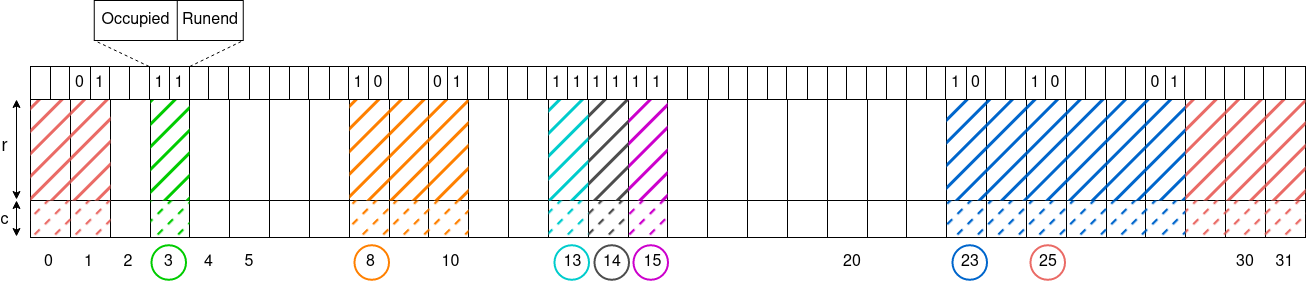
\includegraphics[width=\textwidth]{figures/paperII/example.png}
   \caption{A 32 slots long BQF ($q$=5). First line represents the metadata bits (see~\cite{counting_quotient_filter_2017} for more details). This short example does not represent blocks (\textit{cf.} supplementary data) in the BQF for simplicity. Each slot has a size of $r$ bits for the remainder with $c$ bits for counts and 2 bits of metadata: $occupied$ and $runend$. A circled address $Q$ means that at least one element $x$ such that $h_0(x) = Q$ has been inserted. Multiple remainders sharing the same color in the BQF have been originally inserted at the same address and form a run (\textit{cf.} supplementary data). Empty metadata bits are set to 0.}
   \label{fig:BQF}
\end{figure}

Originally the QF is said to be a probabilistic data structure: with a non-zero false-positive rate when querying elements. In the current framework, as we use an injective hash function, the false-positive rate is zero. However, as explained later (Section \ref{ssec:fimpera}), we use an additional technique that does not exactly query the actual stored elements, and that generates a negligible but non-zero false positive rate at query time.

In practice, the metadata bits used, the probing method and the global organization of the QF we use is based on the Rank \& Select Quotient Filter first proposed in~\cite{counting_quotient_filter_2017}. We detail this structure and the implementation in the Supplementary Materials.


\subsubsection{Abundance in Quotient Filters} 

As previously defined, the Quotient Filter structure is enough to handle the presence or absence of $k$-mers. It is possible to adapt the structure so it can store each $k$-mer alongside with its abundance in the indexed dataset. The Counting Quotient Filter~\cite{counting_quotient_filter_2017} (CQF) is an example of a QF with abundance. 

In the CQF, the abundance of each inserted element can be stored using the following process. A slot is used to store a remainder or an abundance value. If an element $x$ has its abundance $1 \leq n \leq 2$, then the element is inserted $n$ times (with $n=2$, two consecutive slots store $h_1(x)$). When $n > 2$, $h_1(x)$ is stored twice and these two slots act like boundaries in the table, defining the beginning and the end of the counter. Then $n-2$ is encoded and stored between both boundaries, using potentially two slots or more. An extra slot holding a $0$ might be necessary to maintain consistency in the runs. The point here is that this approach uses 2 slots when $n = 2$ and 3 or more when $n > 2$.

In the following section, we present our contribution, called the Backpack Quotient Filter, improving both the way the counts are stored and highly optimizing the size taken by each element to be queried.

\subsection{The Backpack Quotient Filter}\label{ssec:mm:bqf}

\subsubsection{Storing the abundance}
In the BQF, the abundance of each element is stored using the following approach. 
As represented in Figure~\ref{fig:BQF} each slot stores both a remainder and an abundance value. More precisely, each slot stores $r$ bits for the remainder, and $c$ extra bits are used to encode the abundance value. 
The $c$ parameter is a user-defined parameter. The choice of $c$ has a direct impact on the BQF size, adding $c\times 2^q$ bits. The maximum value for abundance is $2^c$ and the value can be an exact count, or an order of magnitude (e.g. encoding of $log_2$ values), offering flexibility based on precision requirements.

If the value of a count overflows the number of bits allocated, the $2^c$ value is stored and the answer at query time is $\ge 2^c$.

Compared to the CQF, the BQF uses only one slot per element, regardless of the abundance of this element, but at the same time it uses more bits per slot. However, thanks to the proposition described in the next section, we can reduce the size of the stored remainder. In this way, we cancel out this effect, even using less space per element while storing abundances.

On a side note, the name Backpack Quotient Filter comes from the fact that every slot handles its own counter, as if it was carrying a backpack.

\subsubsection{Reducing the space usage} \label{ssec:fimpera}

In order to reduce the space usage, we take advantage of a method called Fimpera~\cite{fimpera_2023}. This method is originally
designed to reduce the false-positives of data-structures having non-zero false positive rates. 

Focusing on the presence/absence only, the key idea can be summarized as follows: if a word is present in a text, then all of its sub-words are present. Conversely, if any sub-word is absent, then the whole word is absent. In practice, instead of indexing the $k$-mers from a dataset, we insert all its $s$-mers, with $s\leq k$. At query time a $k$-mer is considered as indexed if and only if all its $s$-mers are indexed in the structure. In the general case of querying a $k$-mer in an structure with collisions, this approach enables to lower the false positive rate of the query because all $s$-mers of a specific $k$-mer need to be false positives to create a false positive $k$-mer. 

The same idea can be exploited when taking the abundance into account. The abundance of a $k$-mer is at most equal to the least abundant $s$-mer it is composed of. Therefore, we store the abundance of s-mers in the filter and report the abundance of a queried k-mer as the minimum of the abundances of the s-mers composing it. The techniques described in~\cite{fimpera_2023} explain how this approach does not have a negative impact on query time and may even improve it.
When applied to a structure having collisions, this approach limits the overestimation of the abundance, as all the $s$-mers of a queried $k$-mer have to be overestimated to overestimate the real abundance of this $k$-mer. 

In the BQF, we do not have any collision. We apply this approach to gain space instead.

Let us first study the size of the reversible hash value, used to store words on a four-character alphabet. Each character (here $\{A,C,G,T\}$) requires two bits for its encoding. Hence, encoding a word of length $\ell$ requires $2\ell$ bits. As we use a reversible hash function, the size of the hash value requires the same size as the original encoded data, $2\ell$. 

By inserting $s$-mers, smaller than $k$-mers, the size of the reversible hash value of each inserted element becomes $2s$ instead of $2k$. If we denote by $z$ the difference between $k$ and $s$, the gain is $2z$ bits per element. In the BQF structure, the consequence is that the size of each slot is decreased by $2z$. All in all, applying this approach enables to save $2^q \times 2z$ bits. The same hash function is used, with the same  properties of injection and reversibility of stored elements.

A drawback of using this approach is the loss of the enumerating feature for $k$-mers. The hash function is still reversible but because we have $s$-mers in the filter, we can only reconstruct (and thus enumerate) these $s$-mers and not the $k$-mers we want to query. It is important to note that we only lose the $k$-mers enumeration, not the dynamicity: resizing the BQF remains possible.

If the counters are not exact, \textit{i.e.} if orders of magnitude are indexed then inserting and deleting new elements is no longer a trivial task. We will study the possibilities of updating the BQF in this case in future work.

The second drawback of applying this approach is the creation of a new kind of false positives, called ``construction false positives''. 
The existence of construction false positive is explained by a simple sentence: a $k$-mer may be absent but all of its $s$-mers may be present. We meet this case if each $s$-mer of an absent $k$-mer $x$ has been individually inserted through the present $k$-mers sharing $s$-mers with $x$. 
Overestimations can also happen, a study of this probability has been realised in fimpera paper~\cite{fimpera_2023}.






\subsubsection{Theoretical influence of the $s$ parameter}\label{ssec:s_influence}
We now detail the theoretical consequences of reducing the size $s$ of indexed elements, with $s \in ]0, k]$. 
\begin{enumerate}
    \item Decreasing $s$ increases the ``construction false positive'' rate.
    The smaller the $s$ value is, the higher is the probability that a queried $k$-mer, non existing in the indexed set, has all its $s$-mers existing in this set. 
    \item Decreasing $s$ may increase the number of indexed $s$-mers in short reads datasets. A sequence of size $\ell$ contains ($\ell-k+1$) $k$-mers and ($\ell-s+1$) $s$-mers. Hence, it contains $z=k-s$ additional $s$-mers than $k$-mers. This is negligible while indexing for instance an assembled genome.
    But when it comes to index millions of reads with low redundancy between them, as this is the case in our experimentations using sea-water metagenomes, each of the million reads contains $z$ more $s$-mers than $k$-mers, with a low redundancy between reads.
    \item Decreasing $s$ decreases the size taken by each indexed $s$-mer, which is the expected effect. This is the main advantage of the approach. Recall that the total size of structure is reduced by $2^q \times 2z$ when using $s$-mers instead of $k$-mers. Hence the smaller $s$ is, the more space is saved.
\end{enumerate}

In general, the results presented Section~\ref{ssec:s_impact} suggest that the size of the data structure decreases as $s$ decreases, despite the conflicting effects of the last two previous points. Selecting small $s$ values only has the potential to increase the construction false positive rate. However, when using recommended values, it stays below $10^{-5}\%$. 

\subsubsection{Doubling the number of slots when the structure is full}\label{sssec:full}
One of the main advantage of building the QF with an injective hash function is that conversely to a Bloom filter for instance, when the structure is full, it is possible to double its number of slots (from $q$ to $q+1$).
During this process, the hash value of each element remains the same, but the way it is distributed between the quotient and remainder changes. This occurs because, after doubling, $q+1$ bits are used to represent the address, while $r-1$ bits are used for the remainder.
Finally, the total number of stored elements faces no theoretical limitation.

In practice, for performances reasons, one doubles the number of slots when the ``load factor'' (number of stored elements divided by the number of slots) becomes bigger than 95\%. Load factor effect experiments have been performed here~\cite{counting_quotient_filter_2017}.


\subsubsection{Number of bits per stored element}\label{sssec:bit_per_element}
As stated, the basis of the QF data structure is to use the address of stored elements as a part of their hash value. As a consequence, the size of the remainder stored for each element decreases when the number of slots increases. This is not linear.  Let us consider the initial scenario, where the QF is composed of $2^q$ slots in which $r$ bits per slot are used as remainder. In this case, the BQF uses $2^q\times(r+c+3)$ bits, as for each stored element, $r$ bits store the remainder, $c$ bits are used to store the abundance, and 3 additional metadata bits are used by the structure itself ($runend$, $occupied$ and a third one, $offset$, explained in supplementary data).

Now consider that the size of the structure doubles in order to index more elements. The structure then contains $2^{q+1}$ slots. In this situation, $q+1$ bits indicate the address of each slot,  and so the remainder of each element decreases to $r-1$ bits instead of $r$. In this case, the total size of the structure becomes $2^{q+1}\times(r-1+c+3) = 2^{q+1}\times(r+c+2)$. As the structure grows, $q+r$ stays constant and the slots become smaller.

Note that this practical effect ends when the remainder is empty, in which case the full hash value of each element is entirely given by the address of the element. This presents a theoretical perspective. In the case of $k$-mer indexing, where conventional $k$ values are typically around 30, approximately 140 petabytes would be needed to contain the $4^k$ slots (representing the number of possible distinct $k$-mers).

\section{Results}
We present experimental results on real metagenomic datasets. The objective is to compare the performances obtained with the BQF with those obtained using state-of-the-art data structures for indexing $k$-mers together with their abundances, based on the Quotient Filter: the CQF~\cite{counting_quotient_filter_2017} and on the counting Bloom Filter: the CBF~\cite{fimpera_2023}. We also included a comparison with Bifrost~\cite{bifrost_2020} and SSHash~\cite{sshash_2023}. Both of these approaches allow for querying indexed $k$-mers, but they have significant differences in their main features, which are summarized below.

These results also enable to show the impact of the unique parameter introduced by BQF: the $s$ value. We also show the influence of the number of indexed elements on the whole data structure size.


The version used for BQF is v1.0.0. Details about protocols and links to datasets are available online~\cite{protocols}.

\subsection{Used datasets} \label{ssec:setup}

Our results were obtained on three distinct metagenomic datasets in which we exclusively considered $k$-mers present two or more times. 

\begin{itemize}
    \item Dataset ``\textit{sea-water34M}'': 34 million Illumina reads from the \textit{Tara} Oceans sequencing project. The uncompressed \textit{fastq} file is  7.7GB. It contains 257M distinct 32-mers and 346M distinct 19-mers occurring at least twice.
    \item Dataset ``\textit{sea-water143M}'': 143 million Illumina reads from the \textit{Tara} Oceans sequencing project. The uncompressed \textit{fastq} file is  33GB. It contains 1.2B distinct 32-mers and 1.5B distinct 19-mers occurring at least twice.
    \item Dataset ``\textit{gut}'': 13 million reads from pig microbiota Pacbio sequencing. The uncompressed \textit{fastq} file is 42GB.  It contains 475M distinct 32-mers and 420M distinct 19-mers occurring at least twice.
\end{itemize}  

These sea-water and gut microbiota metagenomic datasets are representative of a highly complex environment, with a large diversity content. For instance, there are 9.5 billion $k$-mers in \textit{sea-water143M} dataset, leading to a set of 5.7 billion distinct $k$-mers. Among them, only 1.2 billion are present twice or more. For the \textit{gut} dataset, we counted 22 billion $k$-mers, 1.2 billion distinct ones and 0.475 billion are present twice or more. We present in Supplementary Materials a visualisation of the $k$-mer spectrum of the sets \textit{sea-water143M} and \textit{gut}. They illustrate the complexity of these datasets, where there is no peak linked to the specific presence of one or more species. %in A $k$-mer spectrum is available in supplementary materials for a whole visualization. 


\subsection{Compared performances}
In this section, we present a comparative analysis between BQF and CQF (\url{https://github.com/splatlab/cqf}, commit 68939f5). Both structures use the same Xorshift hash function, a PHF, ensuring no collisions. We also compare with results obtained with a counting Bloom filter (CBF), with one hash function, implementing the Fimpera approach (\url{https://github.com/lrobidou/fimpera}, commit 662328d). Both CBF and BQF use 5 bits for counters ($c = 5$), allowing a maximal abundance value of 64 as we store exact values. 
%The objective is to query 32-mers in these datasets, so we have $k=32$. 
BQF and CBF use the Fimpera approach, initialized with $k=32$ and $s=19$, thus 19-mers are counted and inserted. 
The sizes of the BQF and CQF are determined solely by the total number of elements plus the element abundances for the CQF. Regarding the CBF, we decided to create a CBF of the same size as the BQF. This ensures fair comparisons when considering a fixed amount of disk space.
The choice of parameters is discussed further in this section. 

We also show results obtained by Bifrost (version 1.3.1) and SSHash (version 3.0.0). Those comparisons are not exactly fair as these tools embed additional features (computing pre-assembly of the data in the so-called compacted de Bruijn graph, possibly indexing multiple datasets for Bifrost) while Bifrost cannot index the abundance, and while SSHash is a static data structure. However, it is interesting to present these results as they show that these state-of-the-art tools —which are not specifically designed for the task of only indexing $k$-mers with their abundances— are not optimal for this task.
%but they show the limitations of these existing state-of-the art tools in the simple context of indexing only $k$-mers with their abundances.

\subsubsection{Experimental setup}
We computed the build time and the query time for each approach. In addition to the building time, the results show the pre-processing time, \textit{i.e.} the time used to obtain the correct input file from the raw compressed \textit{fastq} file (counted $k$-mers for CQF, CBF and BQF, and SPSSs~\cite{RahmanMedvedevRECOMB20} for SSHash). 

The parameters are $k=32$ for CBF, CQF, and BQF, $c=5$ (counters size for BQF, CBF), and $s=19$ ($19$-mers were inserted for BQF, CBF). For SSHash and Bifrost, we used $k=31$ as using $k=32$ would have doubled the $k$-mer encoding size for Bifrost, and because SSHash uses $k\leq31$. 
%The parameters are $k=32$ for CBF, CQF, and BQF, $k=31$ for SSHash and Bifrost, $c=5$ (counters size for BQF, CBF), and $s=19$ ($19$-mers were inserted for BQF, CBF). 
Bifrost used 4 threads and $m=17$ for SSHash (minimisers size). 

Positive queries in a dataset $\mathcal{D}$ are $k$-mers reads from $\mathcal{D}$ itself. Negative queries are $k$-mers from randomly generated sequences (between 80 and 120 nucleotides). Around 2 billion $k$-mers over 30 million sequences were positively queried. Around 7 billion negative $k$-mers over 100 million sequences were negatively queried. 

BQF and CQF sizes are measured experimentally. Their size corresponds exactly to their theoretical value, also showing that, thanks to the simplicity of the structure, no space overhead is required. CBF size was chosen to be the same as BQF's. SSHash size is the one displayed by the tool at the end of the building step. Bifrost size is measured as the peak memory usage after loading the graph and the index in memory (from binary representation on disk). 

The executions were performed on the GenOuest platform on a node with $4 \times 8$ cores Xeon E5-2660 2,20 GHz with 128 GB of memory.
\subsubsection{Comparative results}
\begin{table}[ht]
\resizebox{\textwidth}{!}{
\begin{tabular}{rr|rrrr|rrr}
Dataset  & Structure & 
\begin{tabular}[c]{@{}r@{}}\textbf{Index size} \\ \textbf{on disk} \\ (GB)\end{tabular}     &   \begin{tabular}[c]{@{}r@{}}\textbf{Bits per }\\ \textbf{element}\end{tabular}   & 
\begin{tabular}[c]{@{}r@{}}Pre-processing +\\Build time (s)\end{tabular}                    &   \begin{tabular}[c]{@{}r@{}} Build \\ peak memory \\ usage (GB) \end{tabular}    & 
\begin{tabular}[c]{@{}r@{}}Pos. query \\ throughput \\ (kmer/s)\end{tabular}                &   \begin{tabular}[c]{@{}r@{}}Neg. query \\ throughput \\ (kmer/s)\end{tabular}    & 
\begin{tabular}[c]{@{}r@{}}FP rate \\ (\%)\end{tabular} \\
    & &      &    &         &         &         &       \\ \hline
    & &      &    &         &         &         &       \\
\textit{sea-water34M}       & Bifrost           & 5.84      & 177   & 1,041$^\alpha$         & 5.84  & 2,687,272     & 3,224,789     & 0     \\
                            & SSHash            & 0.40      & 12    & 1,165$^\beta$ + 67     & 2.46  & 1,150,224     & 1,354,394     &  0     \\ 
                            & {CQF}             & 4.58      & 139   & 215$^\gamma$ + 210     & 4.60  & 1,448,481     & 2,121,294     & 0     \\
                            & CBF               & 1.11      & 26    & 219$^\gamma$ + 429     & 1.11  & 205,306       & 285,061       & $4.8\times10^{-6}$      \\
                            & \textbf{BQF}      & 1.11      & 26    & 219$^\gamma$ + 257     & 1.11  & 2,052,016     & 2,934,776     & $1.6\times10^{-6}$      \\
    & &      &    &         &         &         &       \\ \hline
    & &      &    &         &         &         &       \\
\textit{sea-water143M}      & Bifrost       & 17.57     & 114    & 6,074$^\alpha$          &  21.94  & 1,321,360     & 2,581,435     & 0     \\
                            & SSHash        & 1.97      & 13    & 5,875$^\beta$ + 361      &  11.15  & 871,794       & 1,122,606     & 0      \\
                            & {CQF}         & 17.25     & 113   & 771$^\gamma$ + 949       &  17.52  & 1,097,099     & 1,602,930     & 0     \\
                            & CBF           & 3.93      & 21    & 780$^\gamma$ + 2,039     &  3.93   & 195,177       & 281,244       & $5.8\times10^{-5}$      \\
                            & \textbf{BQF}  & 3.93      & 21    & 780$^\gamma$ + 1,101     &  3.93   & 1,791,640     & 2,616,583     & $3.0\times10^{-5}$        \\
    & &      &    &         &         &         &       \\ \hline 
    & &      &    &         &         &         &       \\
\textit{gut}                & Bifrost           & 5.84      & 99    & 5,972$^\alpha$          &  5.84  & 8,448,220     & 3,114,457     & 0     \\
                            & SSHash            & 0.58      & 10    & 2,558$^\beta$ + 113     &  3.79  & 4,438,401     & 1,286,876     & 0      \\
                            & {CQF}             & 8.90      & 150   & 1,178$^\gamma$ + 396    &  9.01  & 1,598,278     & 1,948,436     & 0     \\
                            & CBF               & 1.11      & 21    & 1,085$^\gamma$ + 468    &  1.11  & 352,201       & 284,545       & $1.6\times10^{-6}$      \\
                            & \textbf{BQF}      & 1.11      & 21    & 1,085$^\gamma$ + 341    &  1.11  & 4,582,535     & 2,821,471     & 0     \\
    & &      &    &         &         &         &       \\ \hline
    \multicolumn{8}{l}{\footnotesize $^\alpha$ Bifrost does not require pre-processing step} \\ 
    \multicolumn{8}{l}{\footnotesize $^\beta$ BCALM~\cite{bcalm_2016} (https://github.com/GATB/bcalm, version 2.2.3) for unitigs + UST~\cite{RahmanMedvedevRECOMB20} (https://github.com/jermp/UST, commit b3d0710) for simplitigs} \\
    \multicolumn{8}{l}{\footnotesize $^\gamma$ KMC~\cite{kmc_2017} (https://github.com/refresh-bio/KMC, version 3.2.4) kmer counting}
\end{tabular} 
}
\caption{Comparative performances. Recall that Bifrost and SSHash do not index the same number of elements than CQF, CBF and BQF, explaining the difference in terms of number of bits per element as compared to the structure size. Given its computation time ($\geq 24$ hours on the \textit{sea-water143M} dataset), we report SSHash results only for the \textit{sea-water34M} dataset. }
\label{table:results}
\end{table}



\paragraph{Comparing CQF and BQF}
Compared to the CQF, the major advantage of the BQF is in terms of space. As shown Table~\ref{table:results}, the BQF is approximately four times smaller than the CQF for every indexed dataset. %at the price of very low false positive rates ($10^{-5}$ or $10^{-6}$\%). 
The same advantage is found in terms of space efficiency (bits/element), being approximately 5 to 7 times more efficient. However, one drawback is the occurrence of false positive calls, which are generally less than $10^{-5}\%$ and can even be as low as 0\% in the gut data set. 

\paragraph{Comparing CBF and BQF}
The results presented Table~\ref{table:results} indicate that the false-positive rate is slightly better with the BQF compared to CBF. However, both approaches still have a very low false positive rate of approximately $10^{-5}$\%, which is insignificant for indexing and pseudo-alignment applications. BQF offers several significant benefits over CBF. First, BQF allows for faster time queries, with an average speed improvement of 50 times compared to CBF. Additionally, BQF does not have any theoretical limitations on the number of stored elements, unlike CBF which is designed for a fixed maximum number of elements that cannot be updated. Finally, the elements stored in a BQF (the $s$-mers) can be enumerated, while this is not the case with the CBF.

\paragraph{Abundance overestimation due to the Fimpera approach}
In this work, we did not recompute the so-called overestimation inherent to the Fimpera abundance representation. This overestimation is in the order of 1\% to 2\% according to the results presented in~\cite{fimpera_2023}, meaning that $1$ to $2$\% of the abundances of true positive calls are overestimated. Furthermore, for those results that were overestimated, the average difference was shown to be approximately 1.07 times the correct abundance range. All in all, this slight overestimation, limited to less than 2\% of the calls, has no significant impact while estimating the abundance of a query composed of at least dozens or hundreds of $k$-mers.

\paragraph{Bifrost and SSHash results}
As shown by results presented Table~\ref{table:results}, Bifrost is approximately two times slower than BQF to build the data structure and more than twice as slow to perform negative queries. It uses approximately 4.5 times more space per element, and more importantly, it does not provide the abundance of $k$-mers. 
The SSHash approach, for its part, taking advantage of super-$k$-mers~\cite{superkmer_2013}, uses approximately 2 times less space per element than BQF. However, it is static and is nearly two orders of magnitude slower to construct, drastically limiting its application to large-scale projects.

\subsection{Impact of size of the indexed $s$-mers}\label{ssec:s_impact}
As stated earlier, the BQF structure stores $s$-mers, to emulate $k$-mers at query time, with $s\leq k$.
The choice of the $s$ value has several consequences that are described Section~\ref{ssec:s_influence}, and that we propose to empirically observe here.


\subsubsection{Effect of $s$ on the number of construction false positives}
\begin{figure}[ht]
    \centering
   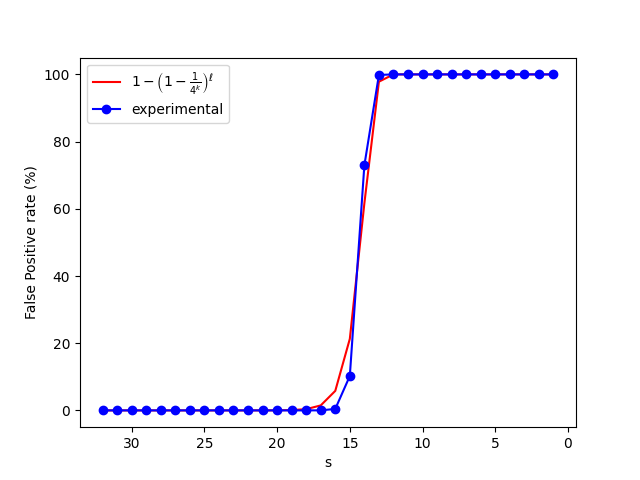
\includegraphics[width=0.75\textwidth]{figures/paperII/fig_fimpera_publi.png}
   \caption{Empirical observation of the evolution of the construction false positive rate with respect to $s$. Indexed dataset: ``\textit{sea-water34M}'', querying random 32-mers. The value of $s$ is decreasing as it starts from $k$, then we increase the difference between $k$ and $s$.}
   \label{fig:fimpera:cfp}
\end{figure}

Figure~\ref{fig:fimpera:cfp} illustrates that using any value of $s$ bigger than 17 enables to limit drastically the construction false positive rate. 
When $s$-mers become smaller than 17 nucleotides, the probability they appear by chance in sequences composed of millions of characters on the $\{A,C,G,T\}$ alphabet becomes close to 1. In this case, mostly any $k$-mers can be constructed from these $s$-mers, explaining the nearly 100\% construction false positive rate.

Note that the shape of this curve is highly correlated with the probability that an element of size $s$ appears by chance in a sequence of size $\ell$. This probability is equal to $1-\left(1-\frac{1}{4^s}\right)^\ell$. In concrete terms, this allows a user to reliably determine a value of $s$ knowing $\ell$, even approximately. The value of $\ell$ can be approximated thanks to the number of distinct $k$-mers in the dataset (as this is the case in Figure~\ref{fig:fimpera:cfp}), efficiently computed by ntCard~\cite{Mohamadi2017ntCardAS} for instance.

These results assume a uniform $ATCG$ distribution, we plan for future work to study the impact of high or low $GC$ content.


\subsubsection{Effect of $s$ on the structure size}
Recall that decreasing $s$ has two opposite effects on the structure size: 
\begin{enumerate}[label=(\alph*)]
    \item in certain conditions (see below), decreasing $s$ can increase the number of indexed $s$-mers, which tends to increase the size of the structure (need to double its size when reaching 95\% load factor);
    \item decreasing $s$ decreases the remainder size, and so decreases the total size of the structure.
\end{enumerate}


\begin{figure}[ht]  
\centering  
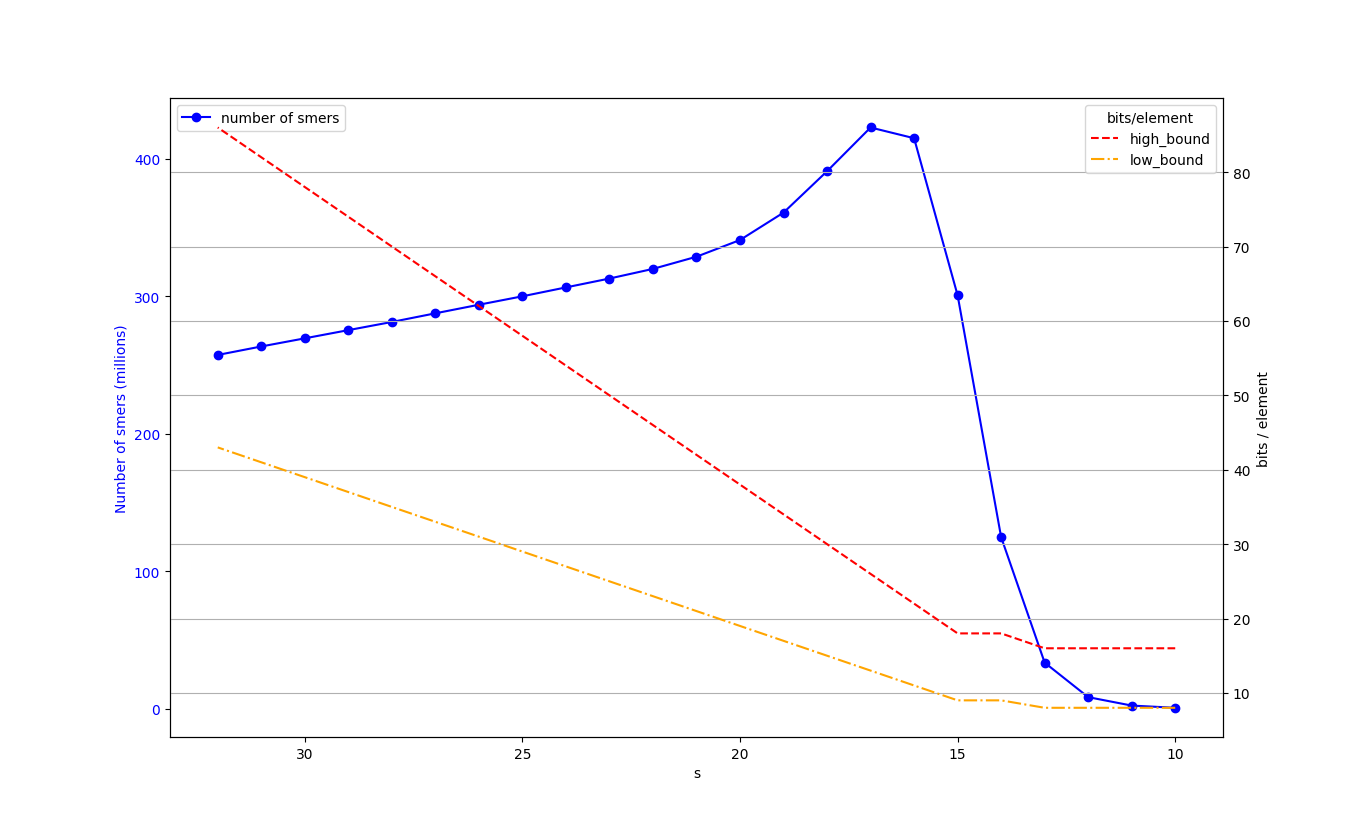
\includegraphics[width=0.95\textwidth]{figures/paperII/fig_limit_fimpera_publi.png}  \hfill  
\caption{Evolution of the number of $s$-mers depending on $s$ in an Illumina sequencing dataset (\textit{sea-water34M}): plain blue line. Evolution of the number of bits per element depending on $s$ on the same dataset. $high\_bound$ is the red upper dotted curve, corresponding to a half-full BQF. $low\_bound$ is plotted in orange, under $high\_bound$ and corresponds to a full BQF ($95\%$ load factor)}
\label{fig:seffect}
\end{figure}

In this section, we propose to observe the practical consequences of this choice.

\noindent(a) Figure~\ref{fig:seffect} shows (plain blue curve) the number of distinct $s$-mers according to $s$. With long enough $s$-mers ($s>17$), decreasing $s$ sub-linearly increases the number of distinct $s$-mers. This is true in the case of relatively short reads, with next generation sequencing for instance (Illumina example within Figure~\ref{fig:seffect} with \textit{sea-water34M} dataset). On the other hand, third-generation sequencing produces longer reads, in this context decreasing $s$ decreases the number of elements to index (475M distinct 32-mers and 420M distinct 19-mers in \textit{gut} PacBio dataset). Table~\ref{table:results} shows this result: when comparing BQF and CQF building time (which depends on the number of elements to index), we can see that BQF is slightly faster on \textit{gut} (PacBio) dataset as there are fewer 19-mers than 32-mers.

With $s\leq 17$, another effect exists: nearly all the $s$-mers exist in the text, and so the number of distinct $s$-mers becomes limited by $4^s$, explaining why the number of distinct $s$-mers decreases when $s$ decreases below $s=17$.
\medskip

\noindent(b) The two dashed lines of Figure~\ref{fig:seffect} show the number of bits per element either if the structure is half full or considered as full (in practice one doubles the structure size if its load factor is 95\%). The observation is that even on this highly complex sea-water metagenomic dataset, the space needed to store $s$-mers decreases when $s$ decreases, even though more $s$-mers have to be stored. A fictitious example is available in the supplementary data, Section ``Side effect of lowering $s$'', demonstrating a case where the number of $s$-mers reaches a doubling threshold before the number of $k$-mers. Results show that, even in this case (increasing number of $s$-mers), the high and low bound of number of bits per element, is never increasing while $s$ decreases.

All in all, regarding the data-structure size, the best choice is to use $s$ as small as possible, but bigger than $17$ to avoid an explosion of the construction false positive rate, as it keeps it below $10^{-5}$\% in this setup. 

\subsection{Effect of the number of indexed elements on the structure size}
\begin{figure}[ht]
\centering
    \makebox[\textwidth]{\makebox[1.30\textwidth]{%
    \begin{minipage}[b]{.55\textwidth}
        \centering
        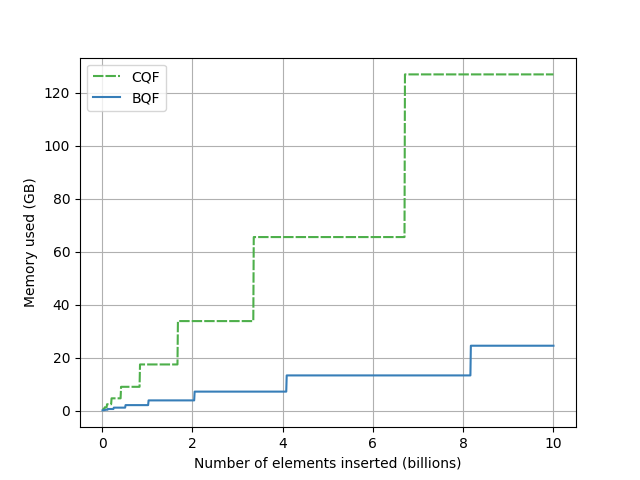
\includegraphics[width=1\textwidth]{figures/paperII/fig_escalier_publi.png}\\
        (A)
    \end{minipage}
    \begin{minipage}[b]{.55\textwidth}
        \centering
        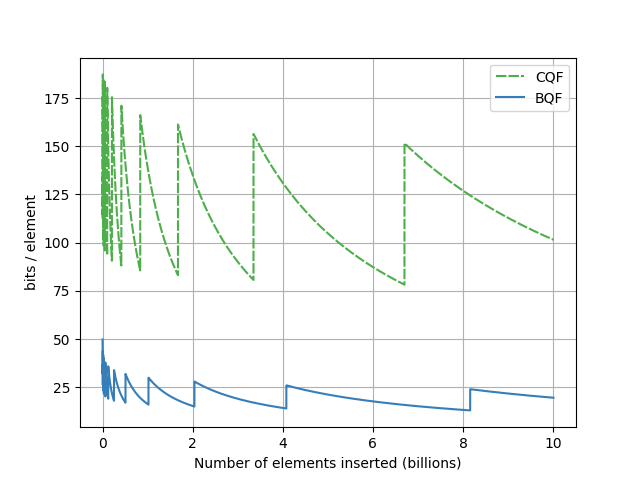
\includegraphics[width=1\textwidth]{figures/paperII/fig_bits_elem_publi.png}\\
        (B)
    \end{minipage}}}
    \caption{Effect of the number of indexed elements on the size and space efficiency. Generated from indexing dataset ``\textit{sea-water34M}'', $k=32$, $s=19$ and $c=5$ for BQF. \textbf{(A)} total data-structure size. \textbf{(B)} size in terms of number of bits per indexed element.}
    \label{fig:size}
\end{figure}


Based on our metagenomic samples, this section comments on the experimental value of bits per element (see section~\ref{sssec:bit_per_element}) used by the BQF compared to CQF. Figure~\ref{fig:size} shows the evolution of the data structure size (A) and the evolution of bits per element (B) while elements are inserted.

The stairs shapes of figure~\ref{fig:size}(A) are due to the size of the data structure that doubles each time their load factor reaches 95\%. Then, each insertion increases the load factor without consuming more space.
The figure highlights the fact that on real metagenomic datasets, the CQF needs a lot of space due to the counter encoding which uses an average of 2.44 slots per element (in the \textit{sea-water34M} dataset). %The BQF, on the other hand, only uses 1 slot, which is a few bits larger than the CQF ones. For a fixed amount of slots, the BQF occupies more space than the CQF. 
Given a fixed number of insertions, because the CQF doubles its size 2.44 times more frequently, the total size occupied by the CQF is much higher than that of the BQF. At least with metagenomics data, while counts are low but not unique, BQF will always occupy less space than CQF.

In figure~\ref{fig:size}(B) the dented curves show the space used per element. The curves are decreasing as the data structures are filled with elements. The vertical jumps correspond to the data structure resizes. We can see that the two structures behave in the same way while the BQF uses fewer bits per element. It is explained by the number of slots per element (a 2.44 times decrease) but also by the Fimpera scheme used in the BQF approach. An interesting fact is that the peaks for both structures get lower while the data structure size doubles. This is because the slots are one bit shorter after each resize, as explained Section~\ref{sssec:bit_per_element}.

Finally, at the price of a negligible non-null false positive rate (in the order of $10^{-5}$\% to $10^{-6}$\% in our experiments), the BQF enables to make queries among dozen of billions of elements, using between 13 and 26 bits per element, while the CQF requires between 75 and 150 bits per element for the same settings.

\section{Conclusion}

This paper introduces the Backpack Quotient Filter, a quotient filter with abundance. The BQF, like other quotient filters, uses a table to store elements. Only a fraction of these elements is explicitly stored, as the rest is implicitly given through their address. Specifically in the BQF, for every element, $c$ additional bits are used to encode the abundance associated. 
This strategy enables to index billions of elements with their abundance using between 13 and 26 bits per element, depending on the data structure load factor.

In addition to this counting strategy, the BQF implements the Fimpera strategy, which emulates $k$-mers from their $s$-mers (with $s\leq k$).
A direct consequence of this emulation is a gain of $2^q \times 2 \times (k-s)$ bits over the whole structure, with $2^q$ being the number of slots in the BQF. Our results show that the results are robust with respect to the $s$ parameter, as long as $s$ is bigger than a fixed threshold, namely $s>17$.

Our results from indexing metagenomic data indicate that the BQF is at least four times more compact than the most similar data structure: the Counting Quotient Filter~\cite{counting_quotient_filter_2017}. The indexing and query times are in the same order of magnitude. This result is at the price of a non-null but extremely low false positive rate ($\approx 10^{-6}$\% in our experiment).
To fully benefit from the flexible sizes of the counters, if the user can afford it, it is advised to index orders of magnitude (e.g. $log_2$ values) instead of exact counts. 

The BQF inserts hash values of the elements. 
By using a perfect hash function, we ensure having no collisions among stored elements. This offers the possibility to enumerate the elements stored in the structure. If the structure gets full when adding elements, this offers a way to relocate all elements after doubling the size of the structure. So there is no theoretical limit to the number of elements stored in the BQF. This dynamicity is significant in the context of intensive sequencing and indexing. 

\begin{subappendices}             % Appendix for this chapter/paper only
    \section{First Subappendix}
    \label[appendix]{sec:sub-app} % Optional argument: Correct cross reference
    \kant[15]                     % Dummy text
\end{subappendices}


%% Format bibliography like a section, not a chapter:
%\printbibliography[heading = subbibliography]

    \appendix           % "Chapter" is renamed "Appendix"
    \appendixpage       % Similar to \part*{Appendices}, but appears in TOC

    % \chapter{The First Appendix}
\label{app:first-app}
\kant[20-21] % Dummy text
\section{First Section}
\kant[22]    % Dummy text
\section{Second Section}
\kant[23-24] % Dummy text
    % \chapter{Source Code}
\label{app:source}
\section{Implementation}
The \texttt{phduio} class is implemented in the following way:
\lstinputlisting[language = {[LaTeX]{TeX}}]{phduio.cls}
    %\printbibliography


\end{document}